% **************************************************************************************************************
% A Classic Thesis Style
% An Homage to The Elements of Typographic Style
%
% Copyright (C) 2018 André Miede and Ivo Pletikosić
%
% If you like the style then I would appreciate a postcard. My address
% can be found in the file ClassicThesis.pdf. A collection of the
% postcards I received so far is available online at
% http://postcards.miede.de
%
% License:
% This program is free software; you can redistribute it and/or modify
% it under the terms of the GNU General Public License as published by
% the Free Software Foundation; either version 2 of the License, or
% (at your option) any later version.
%
% This program is distributed in the hope that it will be useful,
% but WITHOUT ANY WARRANTY; without even the implied warranty of
% MERCHANTABILITY or FITNESS FOR A PARTICULAR PURPOSE.  See the
% GNU General Public License for more details.
%
% You should have received a copy of the GNU General Public License
% along with this program; see the file COPYING.  If not, write to
% the Free Software Foundation, Inc., 59 Temple Place - Suite 330,
% Boston, MA 02111-1307, USA.
%
% PLEASE SEE ALSO THE AUTHORS' NOTE REGARDING THIS LICENSE
% IN THE DOCUMENTATION (ClassicThesis.pdf --> Chapter 1 / Chapter01.tex)
% **************************************************************************************************************
\RequirePackage{silence} % :-\
    \WarningFilter{scrreprt}{Usage of package `titlesec'}
    %\WarningFilter{scrreprt}{Activating an ugly workaround}
    \WarningFilter{titlesec}{Non standard sectioning command detected}
\documentclass[ twoside,openright,titlepage,numbers=noenddot,%1headlines,
                headinclude,footinclude,cleardoublepage=empty,abstract=on,
                BCOR=5mm,paper=a4,fontsize=11pt
                ]{scrreprt}

%********************************************************************
% Note: Make all your adjustments in here
%*******************************************************
% ****************************************************************************************************
% classicthesis-config.tex
% formerly known as loadpackages.sty, classicthesis-ldpkg.sty, and classicthesis-preamble.sty
% Use it at the beginning of your ClassicThesis.tex, or as a LaTeX Preamble
% in your ClassicThesis.{tex,lyx} with % ****************************************************************************************************
% classicthesis-config.tex
% formerly known as loadpackages.sty, classicthesis-ldpkg.sty, and classicthesis-preamble.sty
% Use it at the beginning of your ClassicThesis.tex, or as a LaTeX Preamble
% in your ClassicThesis.{tex,lyx} with % ****************************************************************************************************
% classicthesis-config.tex
% formerly known as loadpackages.sty, classicthesis-ldpkg.sty, and classicthesis-preamble.sty
% Use it at the beginning of your ClassicThesis.tex, or as a LaTeX Preamble
% in your ClassicThesis.{tex,lyx} with \input{classicthesis-config}
% ****************************************************************************************************
% If you like the classicthesis, then I would appreciate a postcard.
% My address can be found in the file ClassicThesis.pdf. A collection
% of the postcards I received so far is available online at
% http://postcards.miede.de
% ****************************************************************************************************


% ****************************************************************************************************
% 0. Set the encoding of your files. UTF-8 is the only sensible encoding nowadays. If you can't read
% äöüßáéçèê∂åëæƒÏ€ then change the encoding setting in your editor, not the line below. If your editor
% does not support utf8 use another editor!
% ****************************************************************************************************
\PassOptionsToPackage{utf8}{inputenc}
  \usepackage{inputenc}

\PassOptionsToPackage{T1}{fontenc} % T2A for cyrillics
  \usepackage{fontenc}


% ****************************************************************************************************
% 1. Configure classicthesis for your needs here, e.g., remove "drafting" below
% in order to deactivate the time-stamp on the pages
% (see ClassicThesis.pdf for more information):
% ****************************************************************************************************
\PassOptionsToPackage{
  drafting=true,    % print version information on the bottom of the pages
  tocaligned=false, % the left column of the toc will be aligned (no indentation)
  dottedtoc=false,  % page numbers in ToC flushed right
  eulerchapternumbers=true, % use AMS Euler for chapter font (otherwise Palatino)
  linedheaders=false,       % chaper headers will have line above and beneath
  floatperchapter=true,     % numbering per chapter for all floats (i.e., Figure 1.1)
  eulermath=false,  % use awesome Euler fonts for mathematical formulae (only with pdfLaTeX)
  beramono=true,    % toggle a nice monospaced font (w/ bold)
  palatino=true,    % deactivate standard font for loading another one, see the last section at the end of this file for suggestions
  style=classicthesis % classicthesis, arsclassica
}{classicthesis}


% ****************************************************************************************************
% 2. Personal data and user ad-hoc commands (insert your own data here)
% ****************************************************************************************************
\newcommand{\myTitle}{A Classic Thesis Style\xspace}
\newcommand{\mySubtitle}{An Homage to The Elements of Typographic Style\xspace}
\newcommand{\myDegree}{Doktor-Ingenieur (Dr.-Ing.)\xspace}
\newcommand{\myName}{André Miede \& Ivo Pletikosić\xspace}
\newcommand{\myProf}{Put name here\xspace}
\newcommand{\myOtherProf}{Put name here\xspace}
\newcommand{\mySupervisor}{Put name here\xspace}
\newcommand{\myFaculty}{Put data here\xspace}
\newcommand{\myDepartment}{Put data here\xspace}
\newcommand{\myUni}{Put data here\xspace}
\newcommand{\myLocation}{Saarbrücken\xspace}
\newcommand{\myTime}{June 2018\xspace}
\newcommand{\myVersion}{\classicthesis}

% ********************************************************************
% Setup, finetuning, and useful commands
% ********************************************************************
\providecommand{\mLyX}{L\kern-.1667em\lower.25em\hbox{Y}\kern-.125emX\@}
\newcommand{\ie}{i.\,e.}
\newcommand{\Ie}{I.\,e.}
\newcommand{\eg}{e.\,g.}
\newcommand{\Eg}{E.\,g.}
% ****************************************************************************************************


% ****************************************************************************************************
% 3. Loading some handy packages
% ****************************************************************************************************
% ********************************************************************
% Packages with options that might require adjustments
% ********************************************************************
\PassOptionsToPackage{ngerman,american}{babel} % change this to your language(s), main language last
% Spanish languages need extra options in order to work with this template
%\PassOptionsToPackage{spanish,es-lcroman}{babel}
    \usepackage{babel}

\usepackage{csquotes}
\PassOptionsToPackage{%
  %backend=biber,bibencoding=utf8, %instead of bibtex
  backend=bibtex8,bibencoding=ascii,%
  language=auto,%
  style=numeric-comp,%
  %style=authoryear-comp, % Author 1999, 2010
  %bibstyle=authoryear,dashed=false, % dashed: substitute rep. author with ---
  sorting=nyt, % name, year, title
  maxbibnames=10, % default: 3, et al.
  %backref=true,%
  natbib=true % natbib compatibility mode (\citep and \citet still work)
}{biblatex}
    \usepackage{biblatex}

\PassOptionsToPackage{fleqn}{amsmath}       % math environments and more by the AMS
  \usepackage{amsmath}

% ********************************************************************
% General useful packages
% ********************************************************************
\usepackage{graphicx} %
\usepackage{scrhack} % fix warnings when using KOMA with listings package
\usepackage{xspace} % to get the spacing after macros right
\PassOptionsToPackage{printonlyused,smaller}{acronym}
  \usepackage{acronym} % nice macros for handling all acronyms in the thesis
  %\renewcommand{\bflabel}[1]{{#1}\hfill} % fix the list of acronyms --> no longer working
  %\renewcommand*{\acsfont}[1]{\textsc{#1}}
  %\renewcommand*{\aclabelfont}[1]{\acsfont{#1}}
  %\def\bflabel#1{{#1\hfill}}
  \def\bflabel#1{{\acsfont{#1}\hfill}}
  \def\aclabelfont#1{\acsfont{#1}}
% ****************************************************************************************************
%\usepackage{pgfplots} % External TikZ/PGF support (thanks to Andreas Nautsch)
%\usetikzlibrary{external}
%\tikzexternalize[mode=list and make, prefix=ext-tikz/]
% ****************************************************************************************************


% ****************************************************************************************************
% 4. Setup floats: tables, (sub)figures, and captions
% ****************************************************************************************************
\usepackage{tabularx} % better tables
  \setlength{\extrarowheight}{3pt} % increase table row height
\newcommand{\tableheadline}[1]{\multicolumn{1}{l}{\spacedlowsmallcaps{#1}}}


\newcommand{\myfloatalign}{\centering} % to be used with each float for alignment
\usepackage{subfig}
% ****************************************************************************************************


% ****************************************************************************************************
% 5. Setup code listings
% ****************************************************************************************************
\usepackage{listings}
%\lstset{emph={trueIndex,root},emphstyle=\color{BlueViolet}}%\underbar} % for special keywords
\lstset{language=[LaTeX]Tex,%C++,
  morekeywords={PassOptionsToPackage,selectlanguage},
  keywordstyle=\color{RoyalBlue},%\bfseries,
  basicstyle=\small\ttfamily,
  %identifierstyle=\color{NavyBlue},
  commentstyle=\color{Green}\ttfamily,
  stringstyle=\rmfamily,
  numbers=none,%left,%
  numberstyle=\scriptsize,%\tiny
  stepnumber=5,
  numbersep=8pt,
  showstringspaces=false,
  breaklines=true,
  %frameround=ftff,
  %frame=single,
  belowcaptionskip=.75\baselineskip
  %frame=L
}
% ****************************************************************************************************


% /* My stuff robintibor@gmail.com */

%\usepackage[textsize=tiny]{todonotes}
\newcommand{\todotext}[1]{\textcolor{red}{TODO: #1}}
\newcommand{\tableheadlinewithwidth}[2]{\multicolumn{1}{p{#1}}{\spacedlowsmallcaps{#2}}}

% ****************************************************************************************************
% 6. Last calls before the bar closes
% ****************************************************************************************************
% ********************************************************************
% Her Majesty herself
% ********************************************************************
\usepackage{classicthesis}


% ********************************************************************
% Fine-tune hyperreferences (hyperref should be called last)
% ********************************************************************
\hypersetup{%
  %draft, % hyperref's draft mode, for printing see below
  colorlinks=true, linktocpage=true, pdfstartpage=3, pdfstartview=FitV,%
  % uncomment the following line if you want to have black links (e.g., for printing)
  %colorlinks=false, linktocpage=false, pdfstartpage=3, pdfstartview=FitV, pdfborder={0 0 0},%
  breaklinks=true, pageanchor=true,%
  pdfpagemode=UseNone, %
  % pdfpagemode=UseOutlines,%
  plainpages=false, bookmarksnumbered, bookmarksopen=true, bookmarksopenlevel=1,%
  hypertexnames=true, pdfhighlight=/O,%nesting=true,%frenchlinks,%
  urlcolor=CTurl, linkcolor=CTlink, citecolor=CTcitation, %pagecolor=RoyalBlue,%
  %urlcolor=Black, linkcolor=Black, citecolor=Black, %pagecolor=Black,%
  pdftitle={\myTitle},%
  pdfauthor={\textcopyright\ \myName, \myUni, \myFaculty},%
  pdfsubject={},%
  pdfkeywords={},%
  pdfcreator={pdfLaTeX},%
  pdfproducer={LaTeX with hyperref and classicthesis}%
}


% ********************************************************************
% Setup autoreferences (hyperref and babel)
% ********************************************************************
% There are some issues regarding autorefnames
% http://www.tex.ac.uk/cgi-bin/texfaq2html?label=latexwords
% you have to redefine the macros for the
% language you use, e.g., american, ngerman
% (as chosen when loading babel/AtBeginDocument)
% ********************************************************************
\makeatletter
\@ifpackageloaded{babel}%
  {%
    \addto\extrasamerican{%
      \renewcommand*{\figureautorefname}{Figure}%
      \renewcommand*{\tableautorefname}{Table}%
      \renewcommand*{\partautorefname}{Part}%
      \renewcommand*{\chapterautorefname}{Chapter}%
      \renewcommand*{\sectionautorefname}{Section}%
      \renewcommand*{\subsectionautorefname}{Section}%
      \renewcommand*{\subsubsectionautorefname}{Section}%
    }%
    \addto\extrasngerman{%
      \renewcommand*{\paragraphautorefname}{Absatz}%
      \renewcommand*{\subparagraphautorefname}{Unterabsatz}%
      \renewcommand*{\footnoteautorefname}{Fu\"snote}%
      \renewcommand*{\FancyVerbLineautorefname}{Zeile}%
      \renewcommand*{\theoremautorefname}{Theorem}%
      \renewcommand*{\appendixautorefname}{Anhang}%
      \renewcommand*{\equationautorefname}{Gleichung}%
      \renewcommand*{\itemautorefname}{Punkt}%
    }%
      % Fix to getting autorefs for subfigures right (thanks to Belinda Vogt for changing the definition)
      \providecommand{\subfigureautorefname}{\figureautorefname}%
    }{\relax}
\makeatother


% /* More my stuff robintibor@gmail.com */
\usepackage{cleveref}
\usepackage{pdflscape}
\usepackage{longtable}
\definecolor{commentcolor}{RGB}{70,130,180}
% \usepackage{amsmath}
\DeclareMathOperator*{\argmax}{arg\,max}
\DeclareMathOperator*{\argmin}{arg\,min}
% ********************************************************************
% Development Stuff
% ********************************************************************
\listfiles
%\PassOptionsToPackage{l2tabu,orthodox,abort}{nag}
%  \usepackage{nag}
%\PassOptionsToPackage{warning, all}{onlyamsmath}
%  \usepackage{onlyamsmath}


% ****************************************************************************************************
% 7. Further adjustments (experimental)
% ****************************************************************************************************
% ********************************************************************
% Changing the text area
% ********************************************************************
%\areaset[current]{312pt}{761pt} % 686 (factor 2.2) + 33 head + 42 head \the\footskip
%\setlength{\marginparwidth}{7em}%
%\setlength{\marginparsep}{2em}%

% ********************************************************************
% Using different fonts
% ********************************************************************
%\usepackage[oldstylenums]{kpfonts} % oldstyle notextcomp
% \usepackage[osf]{libertine}
%\usepackage[light,condensed,math]{iwona}
%\renewcommand{\sfdefault}{iwona}
%\usepackage{lmodern} % <-- no osf support :-(
%\usepackage{cfr-lm} %
%\usepackage[urw-garamond]{mathdesign} <-- no osf support :-(
%\usepackage[default,osfigures]{opensans} % scale=0.95
%\usepackage[sfdefault]{FiraSans}
% \usepackage[opticals,mathlf]{MinionPro} % onlytext
% ********************************************************************
%\usepackage[largesc,osf]{newpxtext}
%\linespread{1.05} % a bit more for Palatino
% Used to fix these:
% https://bitbucket.org/amiede/classicthesis/issues/139/italics-in-pallatino-capitals-chapter
% https://bitbucket.org/amiede/classicthesis/issues/45/problema-testatine-su-classicthesis-style
% ********************************************************************
% ****************************************************************************************************

% ****************************************************************************************************
% If you like the classicthesis, then I would appreciate a postcard.
% My address can be found in the file ClassicThesis.pdf. A collection
% of the postcards I received so far is available online at
% http://postcards.miede.de
% ****************************************************************************************************


% ****************************************************************************************************
% 0. Set the encoding of your files. UTF-8 is the only sensible encoding nowadays. If you can't read
% äöüßáéçèê∂åëæƒÏ€ then change the encoding setting in your editor, not the line below. If your editor
% does not support utf8 use another editor!
% ****************************************************************************************************
\PassOptionsToPackage{utf8}{inputenc}
  \usepackage{inputenc}

\PassOptionsToPackage{T1}{fontenc} % T2A for cyrillics
  \usepackage{fontenc}


% ****************************************************************************************************
% 1. Configure classicthesis for your needs here, e.g., remove "drafting" below
% in order to deactivate the time-stamp on the pages
% (see ClassicThesis.pdf for more information):
% ****************************************************************************************************
\PassOptionsToPackage{
  drafting=true,    % print version information on the bottom of the pages
  tocaligned=false, % the left column of the toc will be aligned (no indentation)
  dottedtoc=false,  % page numbers in ToC flushed right
  eulerchapternumbers=true, % use AMS Euler for chapter font (otherwise Palatino)
  linedheaders=false,       % chaper headers will have line above and beneath
  floatperchapter=true,     % numbering per chapter for all floats (i.e., Figure 1.1)
  eulermath=false,  % use awesome Euler fonts for mathematical formulae (only with pdfLaTeX)
  beramono=true,    % toggle a nice monospaced font (w/ bold)
  palatino=true,    % deactivate standard font for loading another one, see the last section at the end of this file for suggestions
  style=classicthesis % classicthesis, arsclassica
}{classicthesis}


% ****************************************************************************************************
% 2. Personal data and user ad-hoc commands (insert your own data here)
% ****************************************************************************************************
\newcommand{\myTitle}{A Classic Thesis Style\xspace}
\newcommand{\mySubtitle}{An Homage to The Elements of Typographic Style\xspace}
\newcommand{\myDegree}{Doktor-Ingenieur (Dr.-Ing.)\xspace}
\newcommand{\myName}{André Miede \& Ivo Pletikosić\xspace}
\newcommand{\myProf}{Put name here\xspace}
\newcommand{\myOtherProf}{Put name here\xspace}
\newcommand{\mySupervisor}{Put name here\xspace}
\newcommand{\myFaculty}{Put data here\xspace}
\newcommand{\myDepartment}{Put data here\xspace}
\newcommand{\myUni}{Put data here\xspace}
\newcommand{\myLocation}{Saarbrücken\xspace}
\newcommand{\myTime}{June 2018\xspace}
\newcommand{\myVersion}{\classicthesis}

% ********************************************************************
% Setup, finetuning, and useful commands
% ********************************************************************
\providecommand{\mLyX}{L\kern-.1667em\lower.25em\hbox{Y}\kern-.125emX\@}
\newcommand{\ie}{i.\,e.}
\newcommand{\Ie}{I.\,e.}
\newcommand{\eg}{e.\,g.}
\newcommand{\Eg}{E.\,g.}
% ****************************************************************************************************


% ****************************************************************************************************
% 3. Loading some handy packages
% ****************************************************************************************************
% ********************************************************************
% Packages with options that might require adjustments
% ********************************************************************
\PassOptionsToPackage{ngerman,american}{babel} % change this to your language(s), main language last
% Spanish languages need extra options in order to work with this template
%\PassOptionsToPackage{spanish,es-lcroman}{babel}
    \usepackage{babel}

\usepackage{csquotes}
\PassOptionsToPackage{%
  %backend=biber,bibencoding=utf8, %instead of bibtex
  backend=bibtex8,bibencoding=ascii,%
  language=auto,%
  style=numeric-comp,%
  %style=authoryear-comp, % Author 1999, 2010
  %bibstyle=authoryear,dashed=false, % dashed: substitute rep. author with ---
  sorting=nyt, % name, year, title
  maxbibnames=10, % default: 3, et al.
  %backref=true,%
  natbib=true % natbib compatibility mode (\citep and \citet still work)
}{biblatex}
    \usepackage{biblatex}

\PassOptionsToPackage{fleqn}{amsmath}       % math environments and more by the AMS
  \usepackage{amsmath}

% ********************************************************************
% General useful packages
% ********************************************************************
\usepackage{graphicx} %
\usepackage{scrhack} % fix warnings when using KOMA with listings package
\usepackage{xspace} % to get the spacing after macros right
\PassOptionsToPackage{printonlyused,smaller}{acronym}
  \usepackage{acronym} % nice macros for handling all acronyms in the thesis
  %\renewcommand{\bflabel}[1]{{#1}\hfill} % fix the list of acronyms --> no longer working
  %\renewcommand*{\acsfont}[1]{\textsc{#1}}
  %\renewcommand*{\aclabelfont}[1]{\acsfont{#1}}
  %\def\bflabel#1{{#1\hfill}}
  \def\bflabel#1{{\acsfont{#1}\hfill}}
  \def\aclabelfont#1{\acsfont{#1}}
% ****************************************************************************************************
%\usepackage{pgfplots} % External TikZ/PGF support (thanks to Andreas Nautsch)
%\usetikzlibrary{external}
%\tikzexternalize[mode=list and make, prefix=ext-tikz/]
% ****************************************************************************************************


% ****************************************************************************************************
% 4. Setup floats: tables, (sub)figures, and captions
% ****************************************************************************************************
\usepackage{tabularx} % better tables
  \setlength{\extrarowheight}{3pt} % increase table row height
\newcommand{\tableheadline}[1]{\multicolumn{1}{l}{\spacedlowsmallcaps{#1}}}


\newcommand{\myfloatalign}{\centering} % to be used with each float for alignment
\usepackage{subfig}
% ****************************************************************************************************


% ****************************************************************************************************
% 5. Setup code listings
% ****************************************************************************************************
\usepackage{listings}
%\lstset{emph={trueIndex,root},emphstyle=\color{BlueViolet}}%\underbar} % for special keywords
\lstset{language=[LaTeX]Tex,%C++,
  morekeywords={PassOptionsToPackage,selectlanguage},
  keywordstyle=\color{RoyalBlue},%\bfseries,
  basicstyle=\small\ttfamily,
  %identifierstyle=\color{NavyBlue},
  commentstyle=\color{Green}\ttfamily,
  stringstyle=\rmfamily,
  numbers=none,%left,%
  numberstyle=\scriptsize,%\tiny
  stepnumber=5,
  numbersep=8pt,
  showstringspaces=false,
  breaklines=true,
  %frameround=ftff,
  %frame=single,
  belowcaptionskip=.75\baselineskip
  %frame=L
}
% ****************************************************************************************************


% /* My stuff robintibor@gmail.com */

%\usepackage[textsize=tiny]{todonotes}
\newcommand{\todotext}[1]{\textcolor{red}{TODO: #1}}
\newcommand{\tableheadlinewithwidth}[2]{\multicolumn{1}{p{#1}}{\spacedlowsmallcaps{#2}}}

% ****************************************************************************************************
% 6. Last calls before the bar closes
% ****************************************************************************************************
% ********************************************************************
% Her Majesty herself
% ********************************************************************
\usepackage{classicthesis}


% ********************************************************************
% Fine-tune hyperreferences (hyperref should be called last)
% ********************************************************************
\hypersetup{%
  %draft, % hyperref's draft mode, for printing see below
  colorlinks=true, linktocpage=true, pdfstartpage=3, pdfstartview=FitV,%
  % uncomment the following line if you want to have black links (e.g., for printing)
  %colorlinks=false, linktocpage=false, pdfstartpage=3, pdfstartview=FitV, pdfborder={0 0 0},%
  breaklinks=true, pageanchor=true,%
  pdfpagemode=UseNone, %
  % pdfpagemode=UseOutlines,%
  plainpages=false, bookmarksnumbered, bookmarksopen=true, bookmarksopenlevel=1,%
  hypertexnames=true, pdfhighlight=/O,%nesting=true,%frenchlinks,%
  urlcolor=CTurl, linkcolor=CTlink, citecolor=CTcitation, %pagecolor=RoyalBlue,%
  %urlcolor=Black, linkcolor=Black, citecolor=Black, %pagecolor=Black,%
  pdftitle={\myTitle},%
  pdfauthor={\textcopyright\ \myName, \myUni, \myFaculty},%
  pdfsubject={},%
  pdfkeywords={},%
  pdfcreator={pdfLaTeX},%
  pdfproducer={LaTeX with hyperref and classicthesis}%
}


% ********************************************************************
% Setup autoreferences (hyperref and babel)
% ********************************************************************
% There are some issues regarding autorefnames
% http://www.tex.ac.uk/cgi-bin/texfaq2html?label=latexwords
% you have to redefine the macros for the
% language you use, e.g., american, ngerman
% (as chosen when loading babel/AtBeginDocument)
% ********************************************************************
\makeatletter
\@ifpackageloaded{babel}%
  {%
    \addto\extrasamerican{%
      \renewcommand*{\figureautorefname}{Figure}%
      \renewcommand*{\tableautorefname}{Table}%
      \renewcommand*{\partautorefname}{Part}%
      \renewcommand*{\chapterautorefname}{Chapter}%
      \renewcommand*{\sectionautorefname}{Section}%
      \renewcommand*{\subsectionautorefname}{Section}%
      \renewcommand*{\subsubsectionautorefname}{Section}%
    }%
    \addto\extrasngerman{%
      \renewcommand*{\paragraphautorefname}{Absatz}%
      \renewcommand*{\subparagraphautorefname}{Unterabsatz}%
      \renewcommand*{\footnoteautorefname}{Fu\"snote}%
      \renewcommand*{\FancyVerbLineautorefname}{Zeile}%
      \renewcommand*{\theoremautorefname}{Theorem}%
      \renewcommand*{\appendixautorefname}{Anhang}%
      \renewcommand*{\equationautorefname}{Gleichung}%
      \renewcommand*{\itemautorefname}{Punkt}%
    }%
      % Fix to getting autorefs for subfigures right (thanks to Belinda Vogt for changing the definition)
      \providecommand{\subfigureautorefname}{\figureautorefname}%
    }{\relax}
\makeatother


% /* More my stuff robintibor@gmail.com */
\usepackage{cleveref}
\usepackage{pdflscape}
\usepackage{longtable}
\definecolor{commentcolor}{RGB}{70,130,180}
% \usepackage{amsmath}
\DeclareMathOperator*{\argmax}{arg\,max}
\DeclareMathOperator*{\argmin}{arg\,min}
% ********************************************************************
% Development Stuff
% ********************************************************************
\listfiles
%\PassOptionsToPackage{l2tabu,orthodox,abort}{nag}
%  \usepackage{nag}
%\PassOptionsToPackage{warning, all}{onlyamsmath}
%  \usepackage{onlyamsmath}


% ****************************************************************************************************
% 7. Further adjustments (experimental)
% ****************************************************************************************************
% ********************************************************************
% Changing the text area
% ********************************************************************
%\areaset[current]{312pt}{761pt} % 686 (factor 2.2) + 33 head + 42 head \the\footskip
%\setlength{\marginparwidth}{7em}%
%\setlength{\marginparsep}{2em}%

% ********************************************************************
% Using different fonts
% ********************************************************************
%\usepackage[oldstylenums]{kpfonts} % oldstyle notextcomp
% \usepackage[osf]{libertine}
%\usepackage[light,condensed,math]{iwona}
%\renewcommand{\sfdefault}{iwona}
%\usepackage{lmodern} % <-- no osf support :-(
%\usepackage{cfr-lm} %
%\usepackage[urw-garamond]{mathdesign} <-- no osf support :-(
%\usepackage[default,osfigures]{opensans} % scale=0.95
%\usepackage[sfdefault]{FiraSans}
% \usepackage[opticals,mathlf]{MinionPro} % onlytext
% ********************************************************************
%\usepackage[largesc,osf]{newpxtext}
%\linespread{1.05} % a bit more for Palatino
% Used to fix these:
% https://bitbucket.org/amiede/classicthesis/issues/139/italics-in-pallatino-capitals-chapter
% https://bitbucket.org/amiede/classicthesis/issues/45/problema-testatine-su-classicthesis-style
% ********************************************************************
% ****************************************************************************************************

% ****************************************************************************************************
% If you like the classicthesis, then I would appreciate a postcard.
% My address can be found in the file ClassicThesis.pdf. A collection
% of the postcards I received so far is available online at
% http://postcards.miede.de
% ****************************************************************************************************


% ****************************************************************************************************
% 0. Set the encoding of your files. UTF-8 is the only sensible encoding nowadays. If you can't read
% äöüßáéçèê∂åëæƒÏ€ then change the encoding setting in your editor, not the line below. If your editor
% does not support utf8 use another editor!
% ****************************************************************************************************
\PassOptionsToPackage{utf8}{inputenc}
  \usepackage{inputenc}

\PassOptionsToPackage{T1}{fontenc} % T2A for cyrillics
  \usepackage{fontenc}


% ****************************************************************************************************
% 1. Configure classicthesis for your needs here, e.g., remove "drafting" below
% in order to deactivate the time-stamp on the pages
% (see ClassicThesis.pdf for more information):
% ****************************************************************************************************
\PassOptionsToPackage{
  drafting=true,    % print version information on the bottom of the pages
  tocaligned=false, % the left column of the toc will be aligned (no indentation)
  dottedtoc=false,  % page numbers in ToC flushed right
  eulerchapternumbers=true, % use AMS Euler for chapter font (otherwise Palatino)
  linedheaders=false,       % chaper headers will have line above and beneath
  floatperchapter=true,     % numbering per chapter for all floats (i.e., Figure 1.1)
  eulermath=false,  % use awesome Euler fonts for mathematical formulae (only with pdfLaTeX)
  beramono=true,    % toggle a nice monospaced font (w/ bold)
  palatino=true,    % deactivate standard font for loading another one, see the last section at the end of this file for suggestions
  style=classicthesis % classicthesis, arsclassica
}{classicthesis}


% ****************************************************************************************************
% 2. Personal data and user ad-hoc commands (insert your own data here)
% ****************************************************************************************************
\newcommand{\myTitle}{A Classic Thesis Style\xspace}
\newcommand{\mySubtitle}{An Homage to The Elements of Typographic Style\xspace}
\newcommand{\myDegree}{Doktor-Ingenieur (Dr.-Ing.)\xspace}
\newcommand{\myName}{André Miede \& Ivo Pletikosić\xspace}
\newcommand{\myProf}{Put name here\xspace}
\newcommand{\myOtherProf}{Put name here\xspace}
\newcommand{\mySupervisor}{Put name here\xspace}
\newcommand{\myFaculty}{Put data here\xspace}
\newcommand{\myDepartment}{Put data here\xspace}
\newcommand{\myUni}{Put data here\xspace}
\newcommand{\myLocation}{Saarbrücken\xspace}
\newcommand{\myTime}{June 2018\xspace}
\newcommand{\myVersion}{\classicthesis}

% ********************************************************************
% Setup, finetuning, and useful commands
% ********************************************************************
\providecommand{\mLyX}{L\kern-.1667em\lower.25em\hbox{Y}\kern-.125emX\@}
\newcommand{\ie}{i.\,e.}
\newcommand{\Ie}{I.\,e.}
\newcommand{\eg}{e.\,g.}
\newcommand{\Eg}{E.\,g.}
% ****************************************************************************************************


% ****************************************************************************************************
% 3. Loading some handy packages
% ****************************************************************************************************
% ********************************************************************
% Packages with options that might require adjustments
% ********************************************************************
\PassOptionsToPackage{ngerman,american}{babel} % change this to your language(s), main language last
% Spanish languages need extra options in order to work with this template
%\PassOptionsToPackage{spanish,es-lcroman}{babel}
    \usepackage{babel}

\usepackage{csquotes}
\PassOptionsToPackage{%
  %backend=biber,bibencoding=utf8, %instead of bibtex
  backend=bibtex8,bibencoding=ascii,%
  language=auto,%
  style=numeric-comp,%
  %style=authoryear-comp, % Author 1999, 2010
  %bibstyle=authoryear,dashed=false, % dashed: substitute rep. author with ---
  sorting=nyt, % name, year, title
  maxbibnames=10, % default: 3, et al.
  %backref=true,%
  natbib=true % natbib compatibility mode (\citep and \citet still work)
}{biblatex}
    \usepackage{biblatex}

\PassOptionsToPackage{fleqn}{amsmath}       % math environments and more by the AMS
  \usepackage{amsmath}

% ********************************************************************
% General useful packages
% ********************************************************************
\usepackage{graphicx} %
\usepackage{scrhack} % fix warnings when using KOMA with listings package
\usepackage{xspace} % to get the spacing after macros right
\PassOptionsToPackage{printonlyused,smaller}{acronym}
  \usepackage{acronym} % nice macros for handling all acronyms in the thesis
  %\renewcommand{\bflabel}[1]{{#1}\hfill} % fix the list of acronyms --> no longer working
  %\renewcommand*{\acsfont}[1]{\textsc{#1}}
  %\renewcommand*{\aclabelfont}[1]{\acsfont{#1}}
  %\def\bflabel#1{{#1\hfill}}
  \def\bflabel#1{{\acsfont{#1}\hfill}}
  \def\aclabelfont#1{\acsfont{#1}}
% ****************************************************************************************************
%\usepackage{pgfplots} % External TikZ/PGF support (thanks to Andreas Nautsch)
%\usetikzlibrary{external}
%\tikzexternalize[mode=list and make, prefix=ext-tikz/]
% ****************************************************************************************************


% ****************************************************************************************************
% 4. Setup floats: tables, (sub)figures, and captions
% ****************************************************************************************************
\usepackage{tabularx} % better tables
  \setlength{\extrarowheight}{3pt} % increase table row height
\newcommand{\tableheadline}[1]{\multicolumn{1}{l}{\spacedlowsmallcaps{#1}}}


\newcommand{\myfloatalign}{\centering} % to be used with each float for alignment
\usepackage{subfig}
% ****************************************************************************************************


% ****************************************************************************************************
% 5. Setup code listings
% ****************************************************************************************************
\usepackage{listings}
%\lstset{emph={trueIndex,root},emphstyle=\color{BlueViolet}}%\underbar} % for special keywords
\lstset{language=[LaTeX]Tex,%C++,
  morekeywords={PassOptionsToPackage,selectlanguage},
  keywordstyle=\color{RoyalBlue},%\bfseries,
  basicstyle=\small\ttfamily,
  %identifierstyle=\color{NavyBlue},
  commentstyle=\color{Green}\ttfamily,
  stringstyle=\rmfamily,
  numbers=none,%left,%
  numberstyle=\scriptsize,%\tiny
  stepnumber=5,
  numbersep=8pt,
  showstringspaces=false,
  breaklines=true,
  %frameround=ftff,
  %frame=single,
  belowcaptionskip=.75\baselineskip
  %frame=L
}
% ****************************************************************************************************


% /* My stuff robintibor@gmail.com */

%\usepackage[textsize=tiny]{todonotes}
\newcommand{\todotext}[1]{\textcolor{red}{TODO: #1}}
\newcommand{\tableheadlinewithwidth}[2]{\multicolumn{1}{p{#1}}{\spacedlowsmallcaps{#2}}}

% ****************************************************************************************************
% 6. Last calls before the bar closes
% ****************************************************************************************************
% ********************************************************************
% Her Majesty herself
% ********************************************************************
\usepackage{classicthesis}


% ********************************************************************
% Fine-tune hyperreferences (hyperref should be called last)
% ********************************************************************
\hypersetup{%
  %draft, % hyperref's draft mode, for printing see below
  colorlinks=true, linktocpage=true, pdfstartpage=3, pdfstartview=FitV,%
  % uncomment the following line if you want to have black links (e.g., for printing)
  %colorlinks=false, linktocpage=false, pdfstartpage=3, pdfstartview=FitV, pdfborder={0 0 0},%
  breaklinks=true, pageanchor=true,%
  pdfpagemode=UseNone, %
  % pdfpagemode=UseOutlines,%
  plainpages=false, bookmarksnumbered, bookmarksopen=true, bookmarksopenlevel=1,%
  hypertexnames=true, pdfhighlight=/O,%nesting=true,%frenchlinks,%
  urlcolor=CTurl, linkcolor=CTlink, citecolor=CTcitation, %pagecolor=RoyalBlue,%
  %urlcolor=Black, linkcolor=Black, citecolor=Black, %pagecolor=Black,%
  pdftitle={\myTitle},%
  pdfauthor={\textcopyright\ \myName, \myUni, \myFaculty},%
  pdfsubject={},%
  pdfkeywords={},%
  pdfcreator={pdfLaTeX},%
  pdfproducer={LaTeX with hyperref and classicthesis}%
}


% ********************************************************************
% Setup autoreferences (hyperref and babel)
% ********************************************************************
% There are some issues regarding autorefnames
% http://www.tex.ac.uk/cgi-bin/texfaq2html?label=latexwords
% you have to redefine the macros for the
% language you use, e.g., american, ngerman
% (as chosen when loading babel/AtBeginDocument)
% ********************************************************************
\makeatletter
\@ifpackageloaded{babel}%
  {%
    \addto\extrasamerican{%
      \renewcommand*{\figureautorefname}{Figure}%
      \renewcommand*{\tableautorefname}{Table}%
      \renewcommand*{\partautorefname}{Part}%
      \renewcommand*{\chapterautorefname}{Chapter}%
      \renewcommand*{\sectionautorefname}{Section}%
      \renewcommand*{\subsectionautorefname}{Section}%
      \renewcommand*{\subsubsectionautorefname}{Section}%
    }%
    \addto\extrasngerman{%
      \renewcommand*{\paragraphautorefname}{Absatz}%
      \renewcommand*{\subparagraphautorefname}{Unterabsatz}%
      \renewcommand*{\footnoteautorefname}{Fu\"snote}%
      \renewcommand*{\FancyVerbLineautorefname}{Zeile}%
      \renewcommand*{\theoremautorefname}{Theorem}%
      \renewcommand*{\appendixautorefname}{Anhang}%
      \renewcommand*{\equationautorefname}{Gleichung}%
      \renewcommand*{\itemautorefname}{Punkt}%
    }%
      % Fix to getting autorefs for subfigures right (thanks to Belinda Vogt for changing the definition)
      \providecommand{\subfigureautorefname}{\figureautorefname}%
    }{\relax}
\makeatother


% /* More my stuff robintibor@gmail.com */
\usepackage{cleveref}
\usepackage{pdflscape}
\usepackage{longtable}
\definecolor{commentcolor}{RGB}{70,130,180}
% \usepackage{amsmath}
\DeclareMathOperator*{\argmax}{arg\,max}
\DeclareMathOperator*{\argmin}{arg\,min}
% ********************************************************************
% Development Stuff
% ********************************************************************
\listfiles
%\PassOptionsToPackage{l2tabu,orthodox,abort}{nag}
%  \usepackage{nag}
%\PassOptionsToPackage{warning, all}{onlyamsmath}
%  \usepackage{onlyamsmath}


% ****************************************************************************************************
% 7. Further adjustments (experimental)
% ****************************************************************************************************
% ********************************************************************
% Changing the text area
% ********************************************************************
%\areaset[current]{312pt}{761pt} % 686 (factor 2.2) + 33 head + 42 head \the\footskip
%\setlength{\marginparwidth}{7em}%
%\setlength{\marginparsep}{2em}%

% ********************************************************************
% Using different fonts
% ********************************************************************
%\usepackage[oldstylenums]{kpfonts} % oldstyle notextcomp
% \usepackage[osf]{libertine}
%\usepackage[light,condensed,math]{iwona}
%\renewcommand{\sfdefault}{iwona}
%\usepackage{lmodern} % <-- no osf support :-(
%\usepackage{cfr-lm} %
%\usepackage[urw-garamond]{mathdesign} <-- no osf support :-(
%\usepackage[default,osfigures]{opensans} % scale=0.95
%\usepackage[sfdefault]{FiraSans}
% \usepackage[opticals,mathlf]{MinionPro} % onlytext
% ********************************************************************
%\usepackage[largesc,osf]{newpxtext}
%\linespread{1.05} % a bit more for Palatino
% Used to fix these:
% https://bitbucket.org/amiede/classicthesis/issues/139/italics-in-pallatino-capitals-chapter
% https://bitbucket.org/amiede/classicthesis/issues/45/problema-testatine-su-classicthesis-style
% ********************************************************************
% ****************************************************************************************************


%********************************************************************
% Bibliographies
%*******************************************************
%\addbibresource{Bibliography.bib}
\addbibresource{references.bib}
%\addbibresource[label=ownpubs]{AMiede_Publications.bib}

%********************************************************************
% Hyphenation
%*******************************************************
%\hyphenation{put special hyphenation here}

% ********************************************************************
% GO!GO!GO! MOVE IT!
%*******************************************************
\begin{document}
\frenchspacing
\raggedbottom
\selectlanguage{american} % american ngerman
%\renewcommand*{\bibname}{new name}
%\setbibpreamble{}
\pagenumbering{roman}
\pagestyle{plain}
%********************************************************************
% Frontmatter
%*******************************************************
%%*******************************************************
% Little Dirty Titlepage
%*******************************************************
\thispagestyle{empty}
%\pdfbookmark[1]{Titel}{title}
%*******************************************************
\begin{center}
    \spacedlowsmallcaps{\myName} \\ \medskip

    \begingroup
        \color{CTtitle}\spacedallcaps{\myTitle}
    \endgroup
\end{center}

%*******************************************************
% Titlepage
%*******************************************************
\begin{titlepage}
    %\pdfbookmark[1]{\myTitle}{titlepage}
    % if you want the titlepage to be centered, uncomment and fine-tune the line below (KOMA classes environment)
    \begin{addmargin}[-1cm]{-3cm}
    \begin{center}
        \large

        \hfill

        \vfill

        \begingroup
            \color{CTtitle}\spacedallcaps{\myTitle} \\ \bigskip
        \endgroup

        \spacedlowsmallcaps{\myName}

        \vfill

        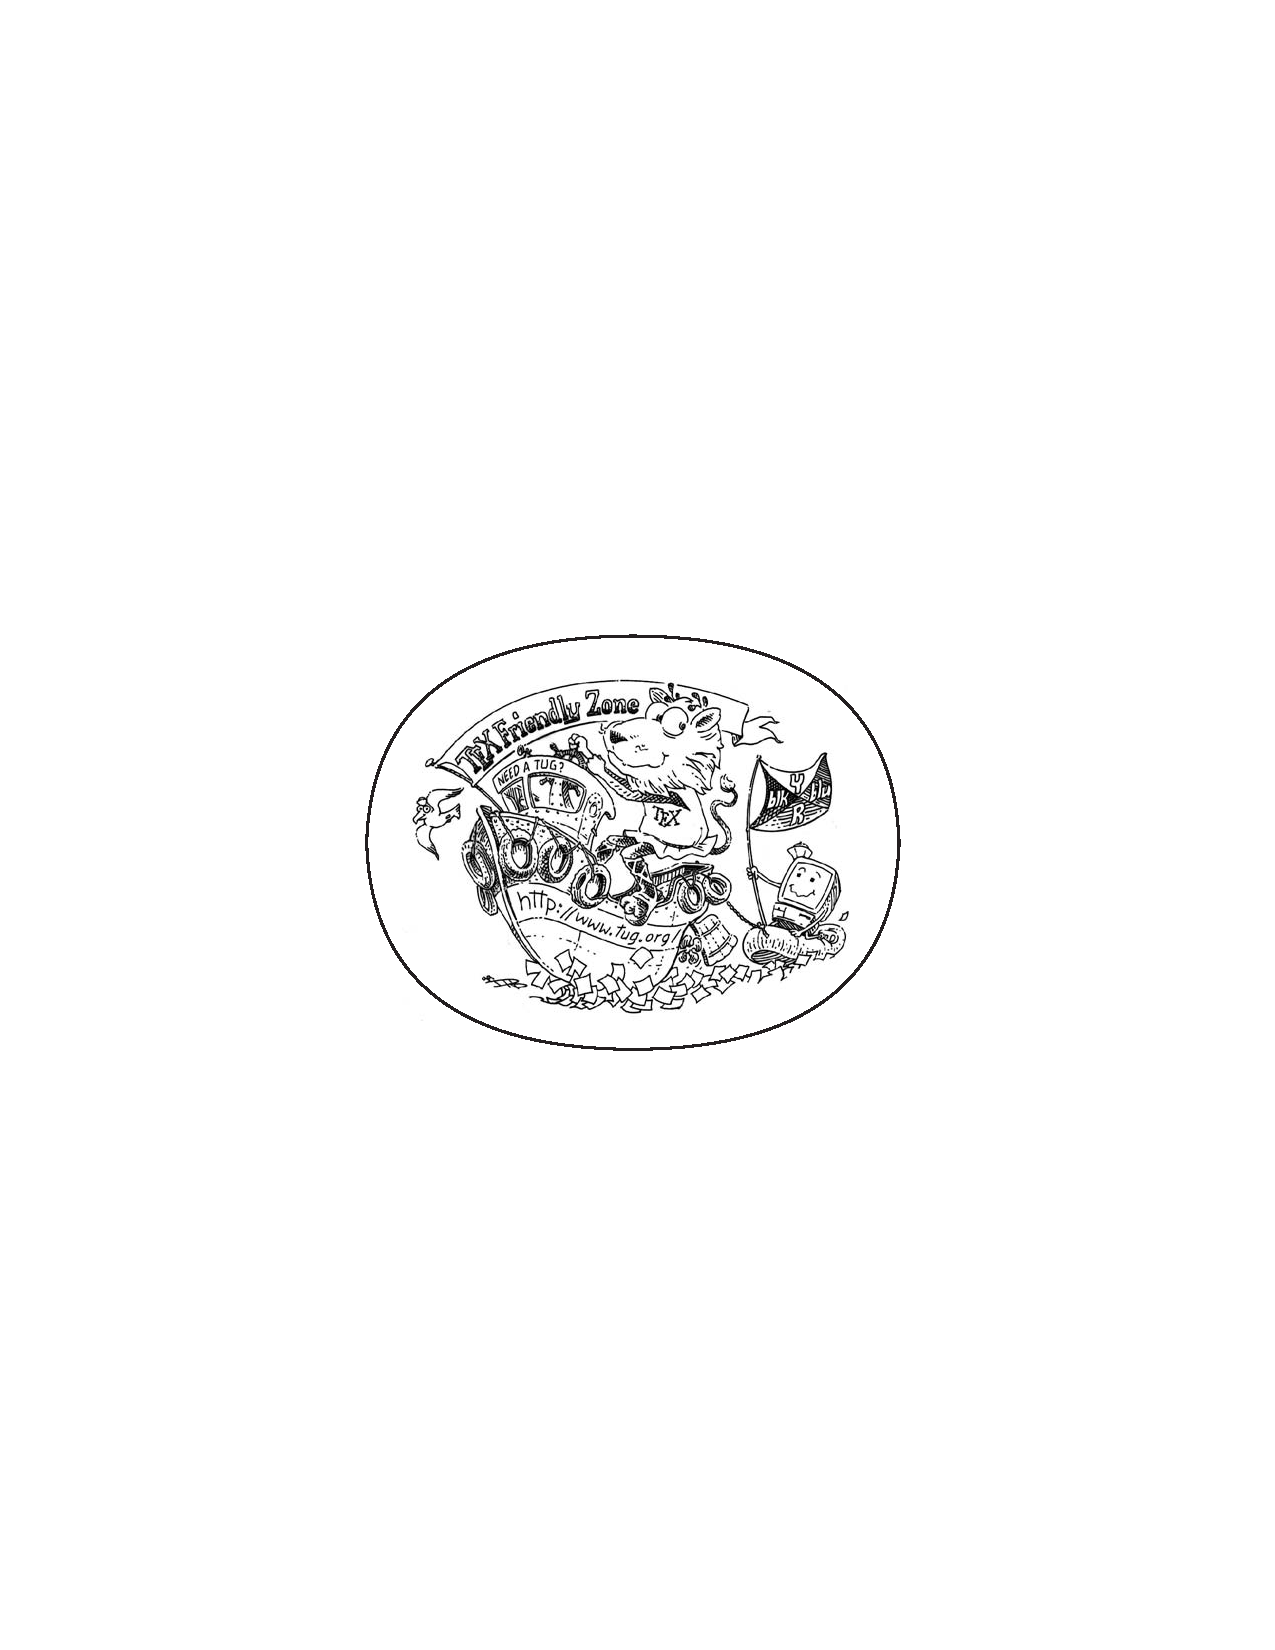
\includegraphics[width=6cm]{gfx/TFZsuperellipse_bw} \\ \medskip

        \mySubtitle \\ \medskip
        %\myDegree \\
        %\myDepartment \\
        %\myFaculty \\
        %\myUni \\ \bigskip

        \myTime\ -- \myVersion

        \vfill

    \end{center}
  \end{addmargin}
\end{titlepage}

\thispagestyle{empty}

\hfill

\vfill


  \begin{flushleft}
   

\noindent\myName: \textit{\myTitle,} \mySubtitle, %\myDegree,
\textcopyright\ \myTime


    

  \end{flushleft}

%\bigskip
%
%\noindent\spacedlowsmallcaps{Supervisors}: \\
%\myProf \\
%\myOtherProf \\
%\mySupervisor
%
%\medskip
%
%\noindent\spacedlowsmallcaps{Location}: \\
%\myLocation
%
%\medskip
%
%\noindent\spacedlowsmallcaps{Time Frame}: \\
%\myTime

%\cleardoublepage%*******************************************************
% Dedication
%*******************************************************
\thispagestyle{empty}
\phantomsection
\pdfbookmark[1]{Dedication}{Dedication}

\vspace*{3cm}

\begin{center}
    \emph{Ohana} means family. \\
    Family means nobody gets left behind, or forgotten. \\ \medskip
    --- Lilo \& Stitch
\end{center}

\medskip

\begin{center}
    Dedicated to the loving memory of Rudolf Miede. \\ \smallskip
    1939\,--\,2005
\end{center}

%\cleardoublepage\include{FrontBackmatter/Foreword}
%\cleardoublepage%*******************************************************
% Abstract
%*******************************************************
%\renewcommand{\abstractname}{Abstract}
\pdfbookmark[1]{Abstract}{Abstract}
% \addcontentsline{toc}{chapter}{\tocEntry{Abstract}}
\begingroup
\let\clearpage\relax
\let\cleardoublepage\relax
\let\cleardoublepage\relax

\chapter*{Abstract}
Machine-learning systems can process larger amounts of brain signals and extract different information from the signals than humans, with potential uses in medical diagnosis or brain-computer interfaces. In particular, brain-signal decoding from electroencephalographic (EEG) recordings is a promising area for machine learning due to the relative ease of acquiring large amounts of EEG recordings and the difficulty of interpreting them manually. To decode EEG signals with machine learning, deep neural networks are a natural choice as they have been successful at a variety of natural-signal decoding tasks like object recognition from images or speech recognition from audio. However, prior to the work in this thesis, it was still unclear how well deep neural networks perform on EEG decoding compared to hand-engineered, feature-based approaches, and more research was needed to determine the optimal approaches for using deep learning to decode EEG. This thesis describes constructing and training deep neural networks for EEG decoding that perform at least as well as feature-based approaches. Visualizations presented in this thesis suggest that deep neural networks learn to extract both well-known physiologically plausible, as well as surprising EEG features.

\vfill
\clearpage
\newpage

\begin{otherlanguage}{ngerman}
\pdfbookmark[1]{Zusammenfassung}{Zusammenfassung}
\chapter*{Zusammenfassung}
Die Dekodierung von Gehirnsignalen mit Hilfe von maschinellem Lernen kann größere Mengen von Signalen verarbeiten und andere Informationen extrahieren als der Mensch, was potenzielle Anwendungen in der medizinischen Diagnose oder bei Gehirn-Computer-Schnittstellen ermöglicht. Insbesondere die Dekodierung von Hirnsignalen aus elektroenzephalographischen (EEG) Aufzeichnungen ist ein vielversprechender Bereich für maschinelles Lernen, da es relativ einfach ist, größere Mengen von EEG-Aufzeichnungen aufzunehmen, und es schwierig ist, diese manuell zu interpretieren. Tiefe neuronale Netze sind eine natürliche Wahl als maschinelles Lernmodell für das Dekodieren von EEG-Signalen, da sie bei einer Vielzahl von Aufgaben zur Dekodierung natürlicher Signale, wie der Objekterkennung aus Bildern oder der Spracherkennung aus Audio, erfolgreich waren. Vor der in dieser Doktoarbeit vorgestellten Forschung war jedoch noch unklar, wie gut tiefe neuronale Netze bei der EEG-Dekodierung im Vergleich zu manuell entwickelten, merkmalsbasierten Ansätzen abschneiden, und es war weitere Forschung erforderlich, um die optimalen Ansätze für die Verwendung von Deep Learning zur EEG-Dekodierung zu ermitteln. In dieser Arbeit wird die Konstruktion und das Training tiefer neuronale Netze für die EEG-Dekodierung beschrieben, die mindestens genauso gut wie merkmalsbasierte Ansätze funktionieren. In dieser Doktorarbeit präsentierte Visualisierungen legen nahe, dass die tiefen neuronalen Netze sowohl bekannte und physiologisch plausible, als auch überraschende EEG-Merkmale extrahieren.
\end{otherlanguage}

\endgroup

\vfill

%\cleardoublepage%*******************************************************
% Publications
%*******************************************************
\pdfbookmark[1]{Publications}{publications}
\chapter*{Publications}

%\noindent Put your publications from the thesis here. The packages \texttt{multibib} or \texttt{bibtopic} etc. can be used to handle multiple different bibliographies in your document.

\begin{refsection}[ownpubs]
    \small
    \nocite{*} % is local to to the enclosing refsection
    \printbibliography[heading=none]
\end{refsection}

%\cleardoublepage%*******************************************************
% Acknowledgments
%*******************************************************
\pdfbookmark[1]{Acknowledgments}{acknowledgments}

\bigskip

\begingroup
\let\clearpage\relax
\let\cleardoublepage\relax
\let\cleardoublepage\relax
\chapter*{Acknowledgments}

I want to thank everybody who supported me emotionally and professionally in the long journey towards this thesis :)

\bigskip
\noindent
Thanks to my family for their encouragements, patience and belief in me.

\bigskip
\noindent
Thanks to all my coworkers and collaborators for providing insights, help and joy during my work.

\bigskip
\noindent
Thanks especially to my supervisors Tonio Ball and Frank Hutter for providing me with the freedom and resources to tackle ambitious research and follow my dream of improving lives by using AI in the medical domain. With your work and expertise we were able to start an intense and impactful research exploration of deep learning on EEG. Let me also thank Jost Tobias Springenberg for his willingness to share his immense deep learning expertise to successfully kickstart my research journey.

\bigskip
\noindent
Thanks to Malak for showing me warmth, joy, love and support in easy and hard times.

\bigskip
\noindent
Thanks to Dephie for showing me the marvelous world, and all her encouragements, ideas, peer coaching, warmth and support.

\bigskip
\noindent
Thanks to Manuel for all his friendship, wisdom, kindness and fun throughout the many years.

\bigskip
\noindent
Thanks to Daniel for all the long-distance telephone support.

\bigskip
\noindent
Thanks to Markus, Jenny, Mirko, Linda, Esin, Edith and all others for providing me with a sense of homecoming on any Berlin trip.

\bigskip
\noindent
Thanks to Raghu for all the sport as well as his puntastic support.

\bigskip
\noindent
Thanks to Lukas and Dan for fruitful discussions and providing a fun atmosphere as officemates.


\bigskip
\noindent
Thanks to all my friends and all who have given me warmth, calmness and supported me in any way.



\bigskip

\endgroup

\cleardoublepage%*******************************************************
% Table of Contents
%*******************************************************
\pagestyle{scrheadings}
%\phantomsection
\pdfbookmark[1]{\contentsname}{tableofcontents}
\setcounter{tocdepth}{2} % <-- 2 includes up to subsections in the ToC
\setcounter{secnumdepth}{3} % <-- 3 numbers up to subsubsections
\manualmark
\markboth{\spacedlowsmallcaps{\contentsname}}{\spacedlowsmallcaps{\contentsname}}
\tableofcontents
\automark[section]{chapter}
\renewcommand{\chaptermark}[1]{\markboth{\spacedlowsmallcaps{#1}}{\spacedlowsmallcaps{#1}}}
\renewcommand{\sectionmark}[1]{\markright{\textsc{\thesection}\enspace\spacedlowsmallcaps{#1}}}
%*******************************************************
% List of Figures and of the Tables
%*******************************************************
\clearpage
% \pagestyle{empty} % Uncomment this line if your lists should not have any headlines with section name and page number
\begingroup
    \let\clearpage\relax
    \let\cleardoublepage\relax
    %*******************************************************
    % List of Figures
    %*******************************************************
    %\phantomsection
    %\addcontentsline{toc}{chapter}{\listfigurename}
    \pdfbookmark[1]{\listfigurename}{lof}
    \listoffigures

    \vspace{8ex}

    %*******************************************************
    % List of Tables
    %*******************************************************
    %\phantomsection
    %\addcontentsline{toc}{chapter}{\listtablename}
    \pdfbookmark[1]{\listtablename}{lot}
    \listoftables

    \vspace{8ex}
    % \newpage

    %*******************************************************
    % List of Listings
    %*******************************************************
    %\phantomsection
    %\addcontentsline{toc}{chapter}{\lstlistlistingname}
    %\pdfbookmark[1]{\lstlistlistingname}{lol}
    %\lstlistoflistings

    %\vspace{8ex}

    %*******************************************************
    % Acronyms
    %*******************************************************
    %\phantomsection
%     \pdfbookmark[1]{Acronyms}{acronyms}
%     \markboth{\spacedlowsmallcaps{Acronyms}}{\spacedlowsmallcaps{Acronyms}}
%     \chapter*{Acronyms}
%     \begin{acronym}[UMLX]
%         \acro{DRY}{Don't Repeat Yourself}
%         \acro{API}{Application Programming Interface}
%         \acro{UML}{Unified Modeling Language}
%     \end{acronym}

\endgroup

%********************************************************************
% Mainmatter
%*******************************************************
\cleardoublepage
\pagestyle{scrheadings}
\pagenumbering{arabic}
%\setcounter{page}{90}
% use \cleardoublepage here to avoid problems with pdfbookmark
\cleardoublepage
%\part{Some Kind of Manual}\label{pt:manual}
%************************************************
\chapter{Introduction}\label{ch:introduction}
%************************************************

\todotext{textbox}

Machine learning (ML), i.e., using data to learn programs that perform a
desired task, has the potential to benefit medical brain-signal-decoding
applications. Compared to humans, machine-learning programs can process
larger amounts of brain-signal data and may extract different
information. For example, machine-learning algorithms have been
developed to help doctors triage patients by quickly detecting stroke
biomarkers from computed tomography (CT)
\citep{chavva2022deep}, to enable brain-computer interfaces
by recognizing people's intentions from electroencephalographic (EEG) in
real time \citep{abiri2019comprehensive} and to detect
pathology from long brain signal recordings
\citep{gemein2020machine,schirrmeisterdeeppathology}. Also,
as brain signals are far from being fully understood, machine-learning
algorithms have the potential to advance scientific understanding by
finding new brain-signal biomarkers for different pathologies
\citep{raghu2020survey}.



    Electroencephalographic (EEG) brain-signal recordings are well-suited
for machine learning since they are easy to acquire, while being
time-consuming and challenging to manually interpret by doctors.
Generating large EEG datasets is relatively simple compared to other
medical recordings because of the low cost and minimal side effects of
performing EEG recordings. Furthermore, EEG recordings are particularly
challenging for humans to interpret, making them a promising target for
information extraction through machine learning. Some clinical
applications of EEG such as pathology diagnosis may be improved by
machine learning, while others such as brain-computer interfaces are
even only possible because of it. Finally, since the information
contained in the EEG signal is far from being fully understood, machine
learning may even help understand the EEG signal itself better.

Deep learning is a very promising approach for brain-signal decoding
from EEG. The term deep learning describes machine-learning models with
multiple computational stages, where the computational stages are
typically trained jointly to solve a given task
\citep{lecun_deep_2015,schmidhuber_deep_2015}.
Convolutional neural networks (ConvNets) are deep learning models that
are inspired by computational structures in the visual cortex of the
brain. ConvNets only have very
general assumptions about the properties of their training signals
embedded into them (such as smoothness and local-to-global hierarchical
structure) and have shown great success on a variety of  decoding tasks 
on natural signals, including object detection in images, speech recognition from audio or machine translation.
Therefore, ConvNets are very promising to apply to hard-to-understand
natural signals like EEG signals.

    Prior to the work presented in this thesis, it was unclear how well
ConvNet architectures can decode EEG signals compared to
hand-engineered, feature-based approaches. The high dimensionality, low
signal-to-noise ratio and large signal variability (e.g., from person to
person or even session to session for the same person) of EEG data
present challenges that may be better addressed by feature-based
approaches that exploit more specific assumptions about the EEG signal.
While there had been previous efforts to apply deep learning to EEG, a
systematic study of the performance of modern ConvNets on EEG decoding
compared with a strong feature-based baseline and including the impact
of network architecture and training hyperparameters, was lacking.
Furthermore, research into understanding what features the ConvNets
extract from the EEG signal had been limited.

    We therefore created several ConvNet architectures to thoroughly
evaluate on EEG decoding. We first evaluated our ConvNet's decoding
performance under a range of different hyperparameter choices on widely
studied movement-related decoding tasks like decoding which limb a
person is thinking of moving. On those tasks, we found our ConvNets to
perform at least as good as a strong feature-based baseline. The
ConvNets also generalized well to a range of other decoding tasks,
including other mental imageries, decoding whether a person made or
perceived an error, as well as pathology diagnosis.

We also developed visualizations to understand the features the ConvNets
extract from the EEG signal, finding that their predictions are
sensitive to plausible neurophysiological features. Using perturbations
of spectral features like amplitude and phase, we show topographies of
the causal effects of spectral changes on the networks predictions. For
decoding of executed movements, these topographies are consistent with
known movement-related spectral brain-signal changes like contralateral
alpha power decreases (e.g., decrease in alpha power on the right side
of the head when moving the left hand). They also suggest that networks
learn to use high-gamma information to predict the performed movement.
Visualizations of inputs that maximally activate specific units in one
of our ConvNets further reveals that the ConvNet has also learned
specific timecourses of amplitude changes, going beyond using just
averaged spectral features.

Later, we more deeply investigated features learned for pathology
decoding. Here, we made use of invertible networks, networks that are
designed such that you can invert intermediate and final network outputs
back to a corresponding input, allowing to visualize output changes in
input space. Further, we also developed a smaller network that is
specifically designed to be interpretable and train it to mimic the
invertible network. Using these methods we could directly show and
investigate temporal waveforms with spatial topographies that are
associated with pathological or healthy recordings. These visualizatiosn
revealed both neurophysiologically plausible features like temporal
slowing as a marker for a pathological EEG or occipital alpha as a
marker for healthy EEG, as well as surprising features like frontal and
temporal very-low-frequency 0.5 Hz components.

    In this thesis, I will first describe the research on deep learning EEG
decoding prior to our work, then proceed to describe the deep network
architectures and training methods we developed to rival or surpass
feature-based EEG decoding approaches on movement- and other
task-related EEG decoding tasks as well as pathology diagnosis.
Furthermore, I also describe the visualization methods we developed that
suggest the networks are using plausible neurophysiological patterns to
solve their tasks. In two separate method and result chapters, I will
delve more deeply into understanding the learned features for pathology
decoding, including by using invertible networks. Finally, I conclude
with my thoughts on the current state of EEG deep learning decoding and
promising avenues for further work like cross-dataset decoding models as
well as models that can process larger timescales of EEG signals.

\todotext{textbox}

%************************************************
\chapter{Prior Work}\label{prior-work}
%**************************************

\begin{startbox}{Research on deep-learning-based EEG decoding was limited prior to our work}
\item Few studies compared results to published feature-based baselines
\item Most EEG deep-learning architectures had only 1-3 convolutional layers and included fully-connected layers with many parameters
\item Most work only considered very restricted frequency ranges
\item Most studies only compared few design choices and training strategies
\end{startbox}


Prior to 2017, when the first work presented in this thesis was
published, there was only limited literature on EEG decoding with deep
learning. In this chapter, I outline what decoding problems, input
representations, network architectures, hyperparameter choices and
visualizations were evaluated in prior work. This is based on the
literature research that we presented in
\citet{schirrmeisterdeephbm2017}.

\section{Decoding Problems and
Baselines}\label{decoding-problems-and-baselines}


% \end{longtable}


\begin{table}[ht]
    \myfloatalign
    \begin{tabularx}{\textwidth}{p{0.5\textwidth}p{0.2\textwidth}p{0.2\textwidth}} \toprule
        \tableheadlinewithwidth{0.5\textwidth}{Decoding problem} & \tableheadlinewithwidth{0.2\textwidth}{Number of studies}
        & \tableheadlinewithwidth{0.2\textwidth}{Published baseline} \\ 
        \midrule
    Imagined or Executed Movement & 6 & 2 \\
    Oddball/P300 & 5 & 1 \\
    Epilepsy-related & 4 & 2 \\
    Music Rhythm & 2 & 0 \\
    Memory Performance/Cognitive Load & 2 & 0 \\
    Driver Performance & 1 & 0 \\
        \bottomrule
    \end{tabularx}
    \caption[Decoding problems in deep-learning EEG decoding studies prior to our work.]{\textbf{Decoding problems in deep-learning EEG decoding studies prior to our work.} Studies with published baseline compared their decoding results to an external baseline result published by other authors.}  \label{prior-work-tasks-table}
\end{table}



    The most widely studied decoding problems were movement-related decoding
problems such as decoding which body part (hand, feet etc.) a person is
moving or imagining to move (see
\Cref{prior-work-tasks-table}). From the 19 studies we
identified at the time, only 5 compared their decoding results to an
external published baseline result, limiting the insights about
deep-learning EEG decoding performance. We therefore decided to compare
deep-learning EEG decoding to a strong feature-based baseline (see
\Cref{fbscp-and-filterbank-net}) on widely researched
movement-related decoding tasks.

\section{Input Domains and Frequency
Ranges}\label{input-domains-and-frequency-ranges}


\begin{figure}[ht]
    \myfloatalign
    %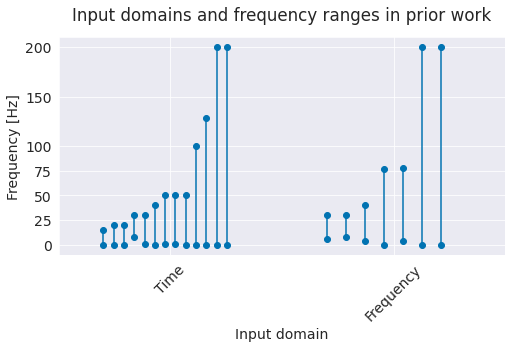
\includegraphics[width=1\linewidth]{latex_images/PriorWork_files/PriorWork_7_0.png}
    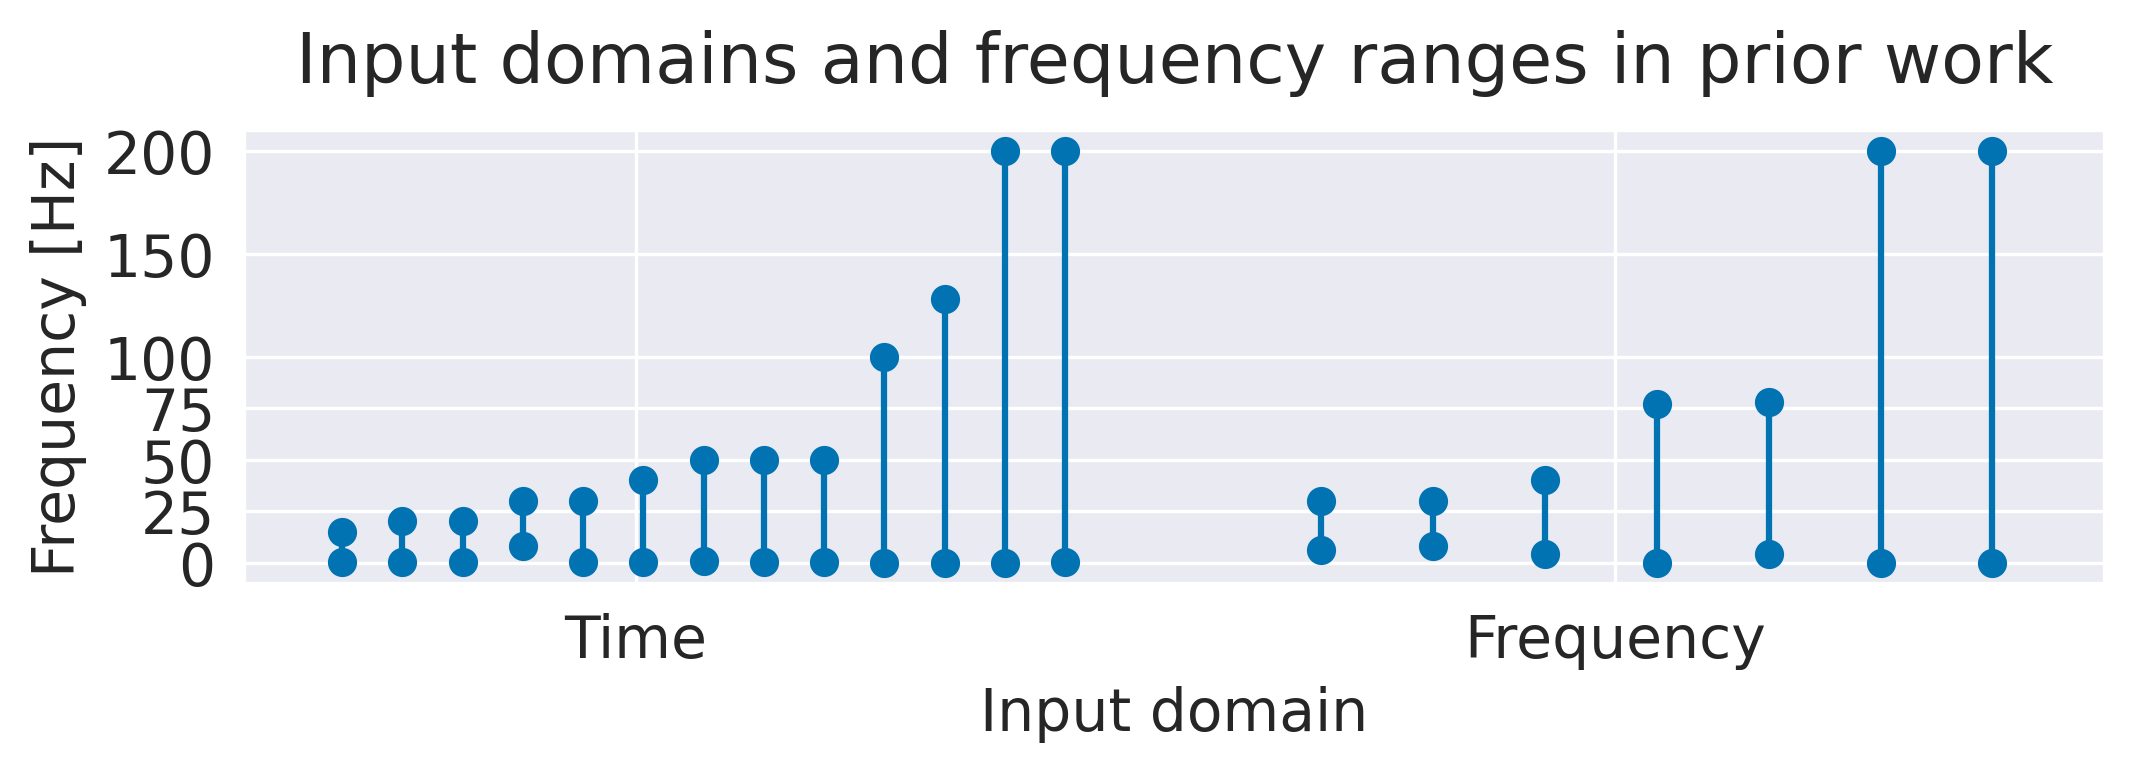
\includegraphics[width=0.9\linewidth,trim={0 0 0 1cm},clip]{images/input-domain-freq-ranges.png}
    \caption[Input domains and frequency ranges in prior work.]{\textbf{Input domains and frequency ranges in prior work.} Lines represent frequency ranges of individual studies. Note that many studies
only include frequencies below 50 Hz, some use very restricted ranges
(alpha/beta band).}\label{input_domain_fig}
\end{figure}
    

    Deep networks can either decode directly from the time-domain EEG or
process the data in the frequency domain, for example after a Fourier
transformation. 12 of the prior studies used time-domain inputs, 6 used
frequency-domain inputs and one used both. We decided to work directly
in the time domain, as the deep networks should in principle be able to
learn how to extract any needed spectral information from the
time-domain input.

Most prior studies that were working in the time domain only used
frequencies below 50 Hz. We were interested in how well deep networks
can also extract higher-frequency components of the EEG
signal. For that, we used a sampling rate of 250 Hz, which means we were
able to analyze frequencies up to the Nyquist frequency of 125 Hz. As a
suitable dataset for high-frequency analysis, we
included our high-gamma dataset in our study, since it was recorded
specifically to allow extraction of higher-frequency (\textgreater50 Hz)
information from scalp EEG \citep{schirrmeisterdeephbm2017}.


\section{Network Architectures}

    

\begin{figure}[ht]
    \myfloatalign
    %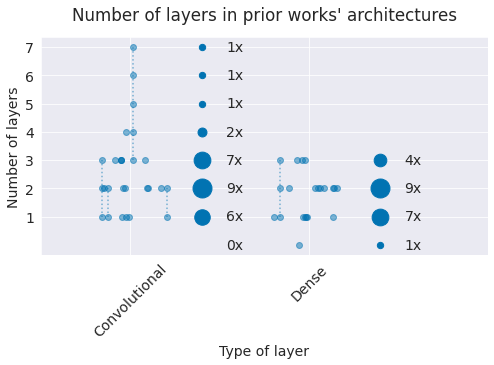
\includegraphics[width=0.9\linewidth]{latex_images/PriorWork_files/PriorWork_11_0.png}
    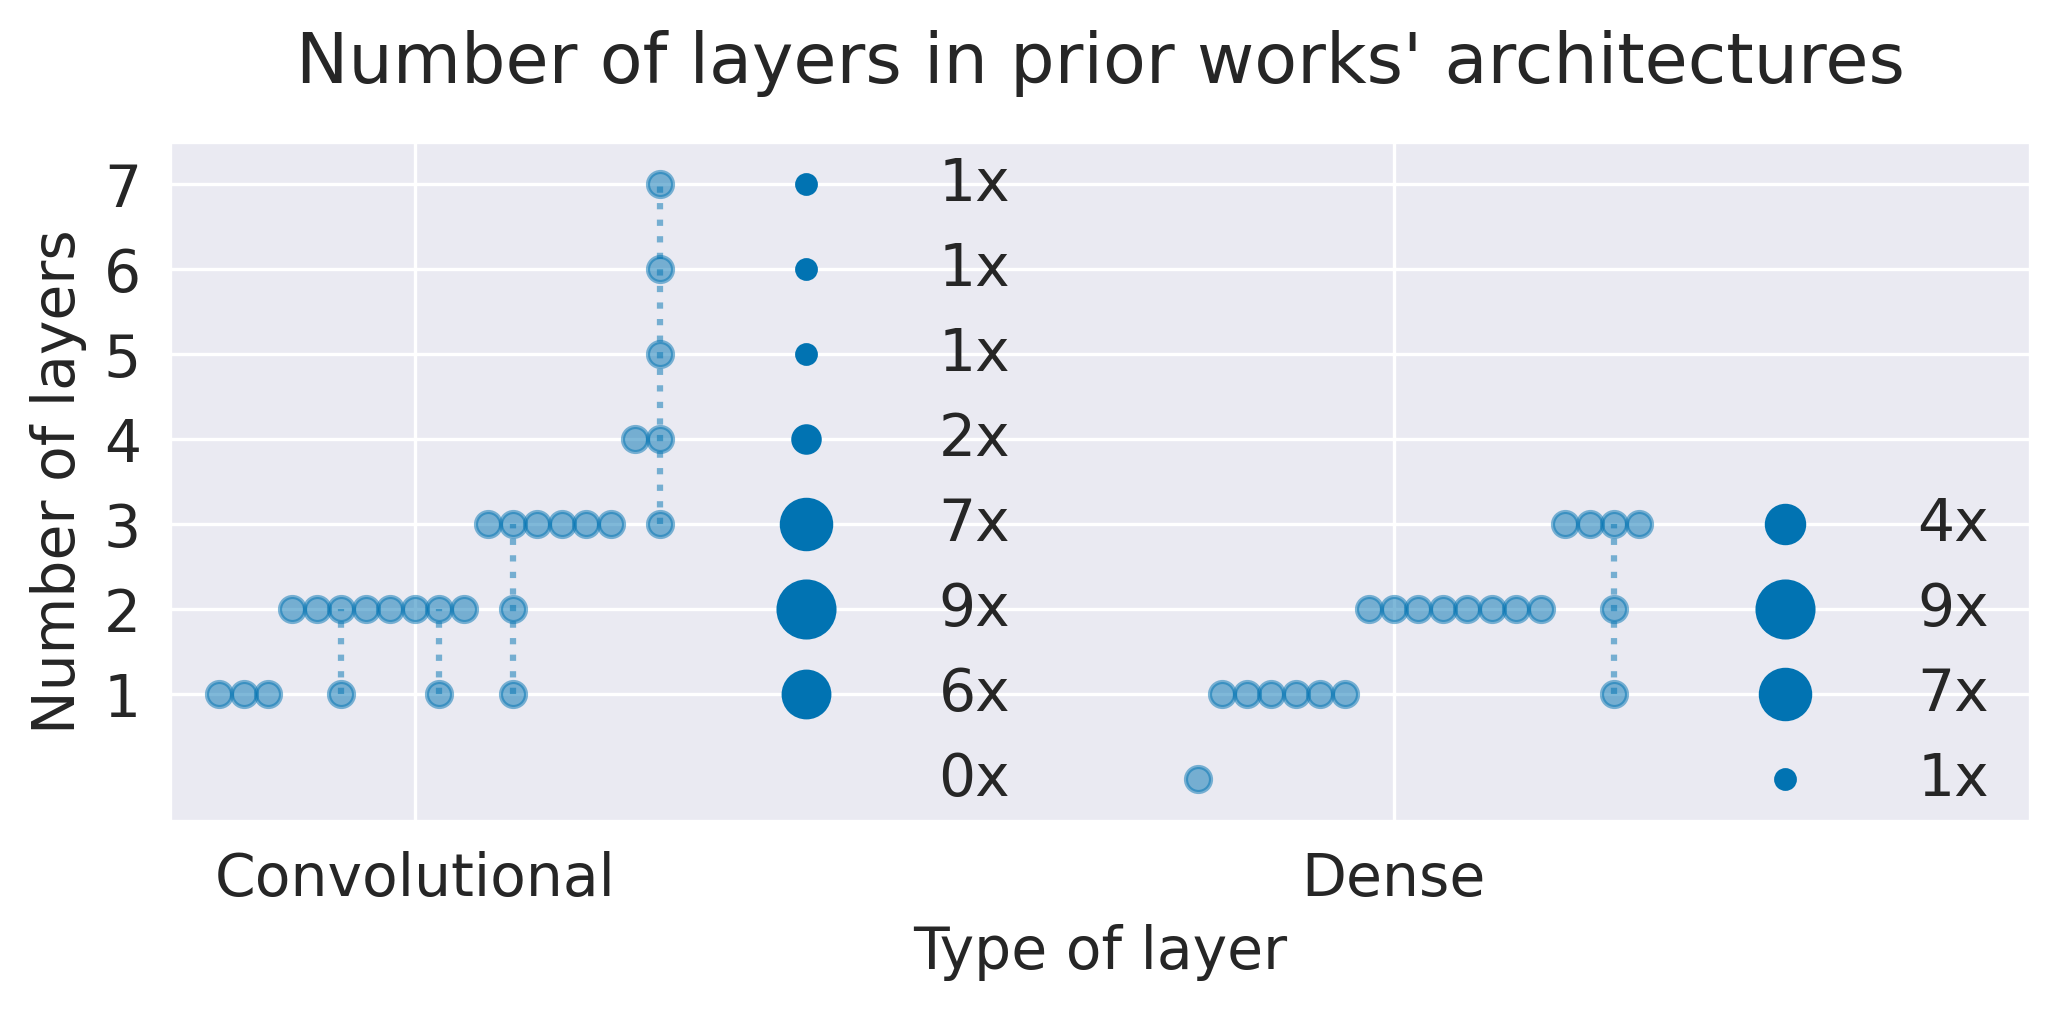
\includegraphics[width=0.9\linewidth,trim={0 0 0 1cm},clip]{images/number-layers.png}
    \caption[Number of layers in prior work.]{
\textbf{Number of layers in prior work.} Small markers represent
individual architectures. Dashed lines indicate different number of
layers investigated in a single study (e.g., a single study investigated
3-7 convolutional layers). Larger markers indicate sum of
occurences of that layer number over all studies (e.g., 9 architectures
used 2 convolutional layers). Note most architectures use only 1-3
convolutional layers.}\label{layernum_fig}
\end{figure}

    The architectures used in prior work typically only included up to 3
layers, with only 2 studies considering more layers. As network
architectures in other domains tend to be a lot deeper, we also
evaluated architectures with a larger number of layers in our work.
Several architectures from prior work also included fully-connected
layers with larger number of parameters which had fallen out of favor in
computer-vision deep-learning architectures due to their large compute
and memory requirements with little accuracy benefit. Our architectures
do not include traditional fully-connected layers with a large number of
parameters.



\section{Hyperparameter Evaluations}\label{hyperparameter-evaluations}

\begin{table}[h!tb]
    \small
    \myfloatalign
    \begin{tabularx}{\textwidth}{p{0.1\textwidth}p{0.4\textwidth}p{0.4\textwidth}} \toprule
        \tableheadlinewithwidth{0.1\textwidth}{\large Study} & \tableheadlinewithwidth{0.4\textwidth}{\large Design choices}
        & \tableheadlinewithwidth{0.4\textwidth}{\large Training strategies} \\ 
        \midrule
    \cite{lawhern_eegnet:_2016} & Kernel sizes & \\
\cite{sun_remembered_2016} & & Different time windows \\
\cite{tabar_novel_2017} & Addition of six-layer stacked
autoencoder on ConvNet features Kernel sizes & \\
\cite{liang_predicting_2016} & & Different subdivisions of
frequency range Different lengths of time crops Transfer learning with
auxiliary non-epilepsy datasets \\
\cite{hajinoroozi_eeg-based_2016} & Replacement of
convolutional layers by restricted Boltzmann machines with slightly
varied network architecture\} & \\
\cite{antoniades_deep_2016} & 1 or 2 convolutional layers
& \\
\cite{page_wearable_2016} & & Cross-subject supervised
training, within-subject finetuning of fully connected layers \\
\cite{bashivan_learning_2016} & Number of convolutional
layers Temporal processing of ConvNet output by max pooling, temporal
convolution, LSTM or temporal convolution + LSTM & \\
\cite{stober_learning_2016} & Kernel sizes & Pretraining
first layer as convolutional autoencoder with different constraints \\
\cite{sakhavi_parallel_2015} & Combination ConvNet and MLP
(trained on different features) vs.~only ConvNet vs.~only MLP & \\
\cite{stober_using_2014} & Best values from automatic
hyperparameter optimization: frequency cutoff, one vs two layers, kernel
sizes, number of channels, pooling width & Best values from automatic
hyperparameter optimization: learning rate, learning rate decay,
momentum, final momentum \\
\cite{wang_deep_2013} & Partially supervised CSA & \\
\cite{cecotti_convolutional_2011} & Electrode subset (fixed
or automatically determined) Using only one spatial filter Different
ensembling strategies & \\
        \bottomrule
    \end{tabularx}
    \caption[Design choices and training strategies of prior work.]{\textbf{Design choices and training strategies of prior work.}}  \label{prior-work-design-choices-table}
\end{table}

    Prior work varied widely in their comparison of design choices and
training strategies. 6 of the studies did not compare any design choices
or training strategy hyperparameters. The other 13 studies evaluated
different hyperparameters, with the most common one the kernel size (see
\Cref{prior-work-design-choices-table}). Only one study
evaluated a wider range of hyperparameters
\citep{stober_using_2014}. To fill this gap, we compared a
wider range of design choices and training strategies and specifically
evaluated whether improvements of computer vision architecture design
choices and training strategies also lead to improvements in EEG
decoding.


\section{Visualizations}\label{visualizations}

\begin{table}[h!tb]
    \small
    \myfloatalign
    \begin{tabularx}{\textwidth}{p{0.1\textwidth}p{0.25\textwidth}p{0.55\textwidth}} \toprule
        \tableheadlinewithwidth{0.1\textwidth}{\large Study} & \tableheadlinewithwidth{0.25\textwidth}{\large Type(s)}
        & \tableheadlinewithwidth{0.55\textwidth}{\large Findings} \\ 
        \midrule
\cite{sun_remembered_2016} & Weights (spatial) & Largest weights found over prefrontal and temporal cortex.\\
\cite{manor_multimodal_2016} & Weights, activations, gradient-based saliency maps & Weights showed typical P300 distribution. Activations were high at plausible times (300-500ms). Saliency maps showed plausible spatio-temporal plots.\\
\cite{tabar_novel_2017} & Weights (spatial + frequential) & Some weights represented difference of values of two electrodes on different sides of head.\\
\cite{liang_predicting_2016} & Weights,
clustering of weights & Clusters of weights showed typical frequency band subdivision (delta, theta, alpha, beta, gamma). \\
\cite{antoniades_deep_2016} & Weights, correlation weights and interictal epileptic discharges (IED), activations & Weights increasingly correlated with IED waveforms with increasing number of training iterations. Second layer captured more complex and well-defined epileptic shapes than first layer. IEDs led to highly synchronized activations for neighbouring electrodes. \\
\cite{thodoroff_learning_2016} & Input occlusion and effect on prediction accuracy & Allowed to locate areas critical for seizure. \\
\cite{george_single-trial_2016} & Weights (spatial) &  Some filter weights had expected topographic distributions for P300, others filters had large weights on areas not traditionally associated with P300.\\
\cite{bashivan_learning_2016} & Inputs that maximally activate given filter; Activations of these inputs, "Deconvolution" for these inputs & Different filters were sensitive to different frequency bands. Later layers had more spatially localized activations. Learned features had noticeable links to well-known electrophysiological markers of cognitive load.\\
\cite{stober_learning_2016} & Weights (spatial+3 timesteps, pretrained as autoencoder) & Different constraints led to different weights, one type of constraints could enforce weights that are similar across subjects. Other type of constraints led to weights that have similar spatial topographies under different architectural configurations and preprocessings. \\
\cite{manor_convolutional_2015} & Weights; Mean and single-trial activations & Spatiotemporal regularization led to softer peaks in weights. Spatial weights showed typical P300 distribution; Activations mostly had peaks at typical times (300-400ms). \\
\cite{cecotti_convolutional_2011} & Weights & Spatial filters were similar for different architectures. Spatial filters were different (more focal, more diffuse) for different subjects. \\
        \bottomrule
    \end{tabularx}
    \caption[Visualizations presented in prior work.]{\textbf{Visualizations presented in prior work.}}  \label{prior-work-visualizations-table}
\end{table}


    Visualizations can help understand what information the networks are
extracting from the EEG signal. 11 of the prior 19 studies presented any
visualizations. These studies mostly focused on analyzing weights and
activations, see \Cref{prior-work-visualizations-table}. In
our work, we first focused on investigating how far the networks extract
spectral features known to work well for movement-related decoding, see
\Cref{perturbation-visualization}. Later, we also developed
more sophisticated visualization methods and applied them both to
pathology decoding, see \Cref{invertible-networks} and
\Cref{understanding-pathology}.

\begin{openbox}
\item How do ConvNets perform on well-researched EEG movement-related decoding tasks against strong feature-based baselines?
\item How do shallower and deeper architectures compare?
\item How do design choices and training strategies affect the decoding performance?
\item What features do the deep networks learn on the EEG signals?
\item Do they learn to use higher-frequency (>50 Hz) information?
\end{openbox}

%************************************************
\chapter{Filter Bank Common Spatial Patterns and
Filterbank Network}\label{ch:fbscp-and-filterbank-net}
%**************************************

\todotext{textbox}


    In a prior master thesis
\citep{schirrmeister_msc_thesis_2015}, we had developed a
neural network architecture closely resembling the feature-based
decoding algorithm filter bank common spatial patterns. In this chapter,
I describe filter bank common spatial patterns as well as the
corresponding filter bank network of the prior master thesis as the
starting point for the network architectures developed in the context of
this thesis.

\section{Filter Bank Common Spatial Patterns as a Starting
Point}\label{filter-bank-common-spatial-patterns-as-a-starting-point}


We selected filter bank common spatial patterns (FBSCP
\cite{ang_filter_2008,chin_multi-class_2009}) as the
feature-based EEG-decoding algorithm we were trying to imitate in our
initial neural network architectures. FBCSP is an EEG-decoding algorithm
that has been successfully used in task-related EEG-decoding
competitions \cite{tangermann_review_2012}. FBCSP aims to
decode task-related changes in signal amplitude in different
frequencies, such as a decrease in the amplitude of alpha and beta-band
oscillations during movement imagination. In the following, we will
explain how FBCSP decodes two classes of EEG signals by finding
frequency-specific spatial filters that transform the signal, such that
the transformed signal has relatively high variance for one class and low variance for the
other class and vice versa.


\section{Common Spatial Patterns}\label{common-spatial-patterns}


\begin{figure}[th]
    \myfloatalign
    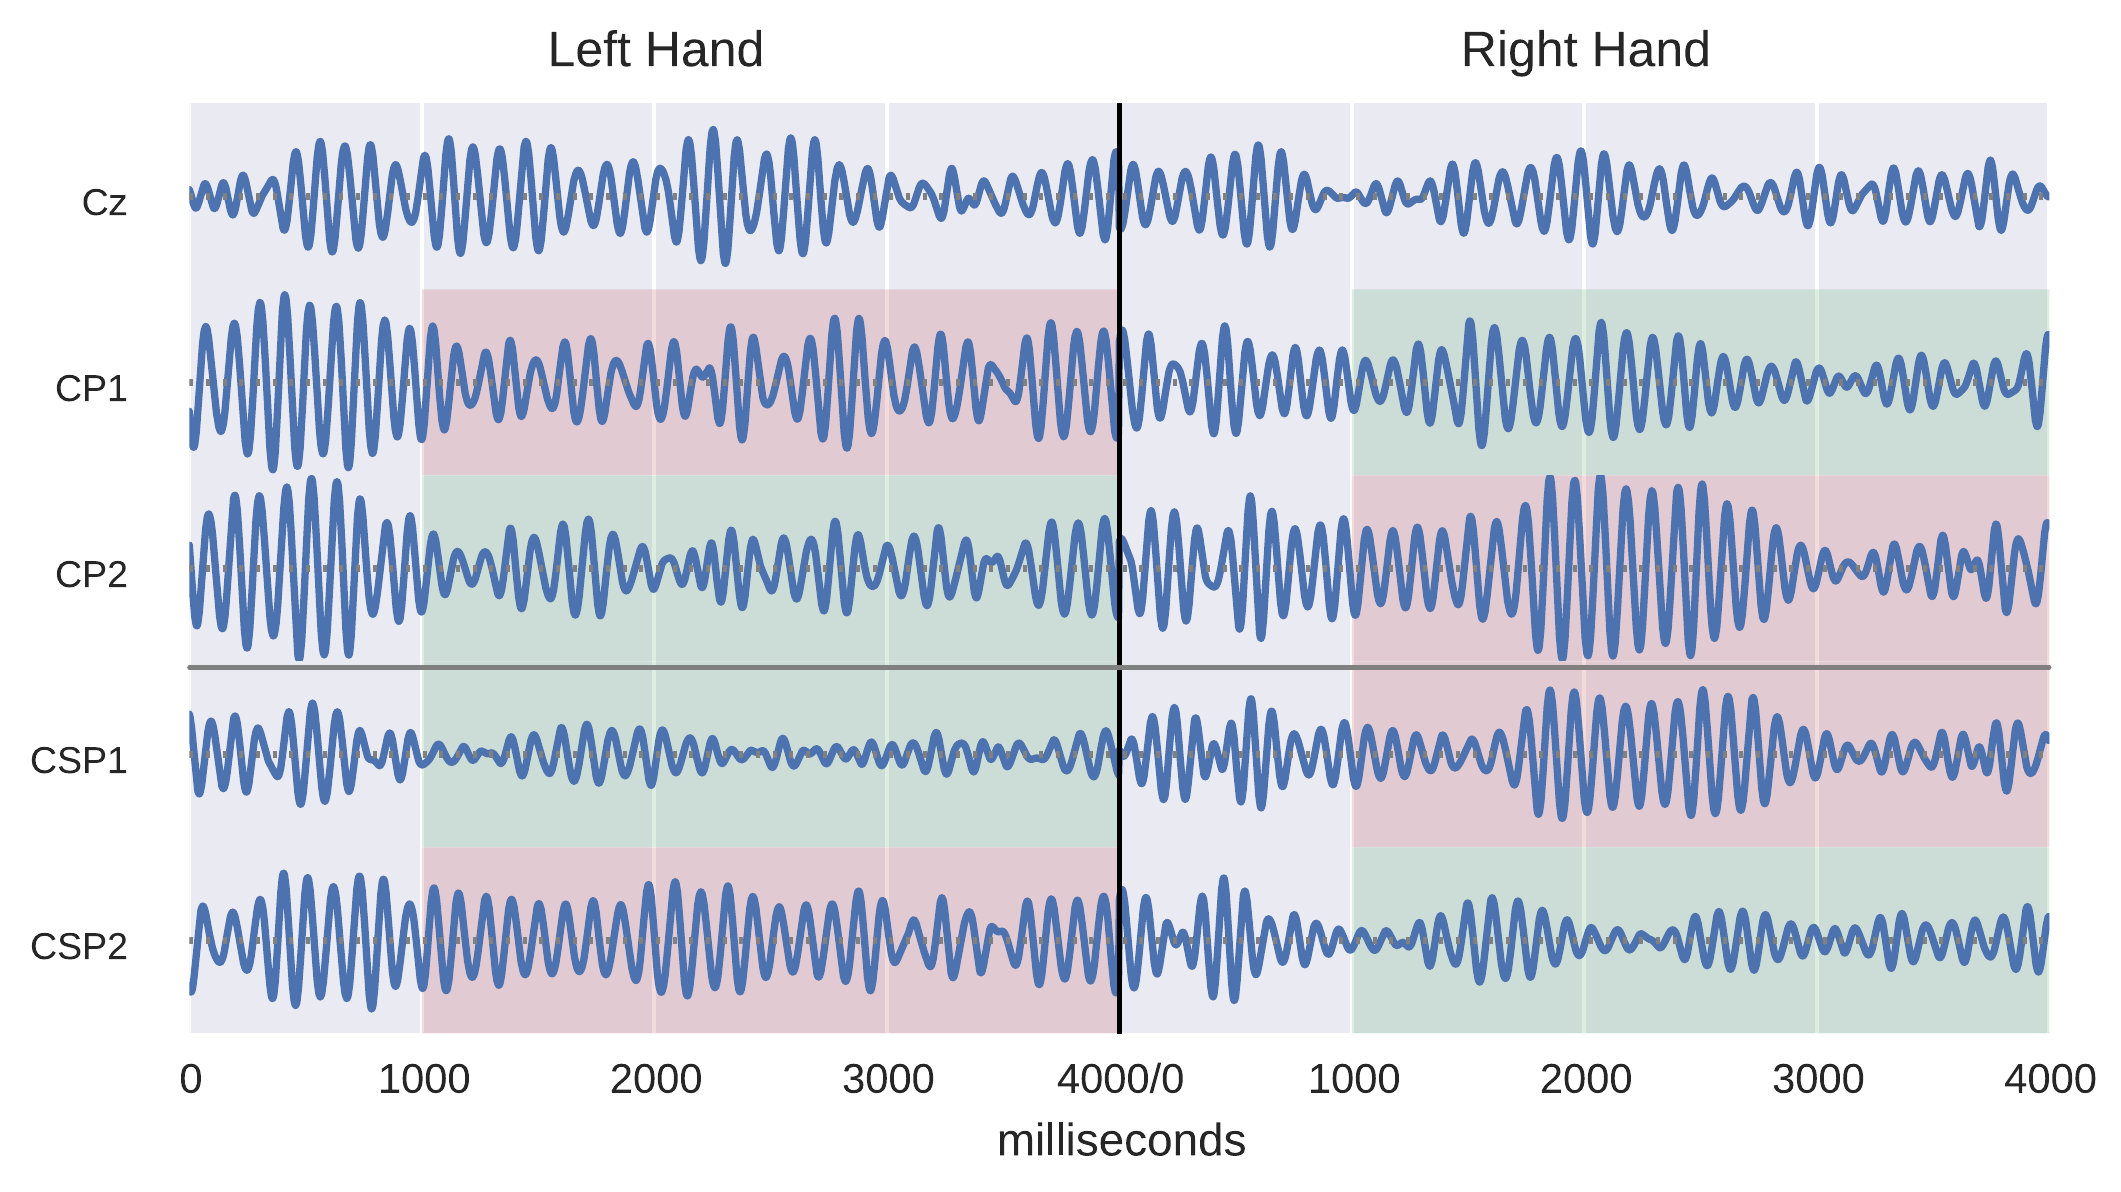
\includegraphics[width=1\linewidth]{images/Methods_Common_Spatial_Patterns_18_0.png}
    \caption[Common Spatial Patterns example.]{
\textbf{Common Spatial Patterns example.} Top parts show EEG
signals for three electrodes during a left hand and a right hand
movement. Bottom parts show spatially filtered signals of two CSP
filters. Green parts have lower variance and red parts have higher
variance. Note that this difference is strongly amplified after CSP
filtering. Figure from prior master thesis
\citep{schirrmeister_msc_thesis_2015}.}\label{csp-figure}
\end{figure}


    The basic building block of FBCSP is the common spatial patterns (CSP)
algorithm. CSP is used to decode neuronal activity that leads to a
change in the amplitudes of the EEG signal with a specific spatial
topography \citep{koles_spatial_1990,ramoser_optimal_2000,blankertz_optimizing_2008}.
To do that, CSP aims to maximize the ratio of the signal variance
between spatially filtered signals of two classes, e.g.~of the signal
during two different movements. For example, the signal of a spatial
filter computed by CSP may have a very large variance during movements
of the left hand and a very small variance during movements of the right
hand. Concretely, we are given signals
$X_{1}, X_{2} \in \mathbb{R}^{n x k x t}$ from $n$ EEG trials (can
be different for $X_1, X_2$, $k$ EEG electrodes and $t$
timepoints within each trial. CSP then finds a spatial filter $w$ that
maximize the ratio of the variances of the spatially filtered
$X_1,X_2$:

\begin{equation*}
w=\argmax_w\frac{Var(w^T X_1)}{Var(w^T X_2)}= \argmax_w\frac{||w^T X_1||^2}{||w^T X_2||^2}=\argmax_w\frac{w^T X_1 X_1^T w}{w^T X_2 X_2^T w}
\end{equation*}

    Rather than just finding a single spatial filter $w$, CSP is typically
used to find a whole matrix of spatial filters $W^{kxk}$, with spatial
filters ordered by the above variance ratio and orthogonal to each
other. The first filter $w_1$ results in the largest variance ratio
and the last filter $w_k$ results in the smallest variance ratio.
Different algorithms can then be used to subselect some set of filters
to filter signals for a subsequent decoding algorithm.

The CSP-filtered signals can be used to construct features to train a
classifier. Since the CSP-filtered signals should have very different
variances for the different classes, the natural choice is to use the
per-trial variances of the CSP-filtered signals as features. This
results in as many features per trial as the number of CSP filters that
were selected for decoding. Typically, one applies the logarithm to the
variances to get more standard-normally distributed features.


\section{Filter Bank Common Spatial
Patterns}\label{filter-bank-common-spatial-patterns}

    CSP is typically applied to an EEG signal that has been bandpass
filtered to a specific frequency range. The filtering to a frequency
range is useful as brain signals cause EEG signal amplitude changes that
are temporally and spatially different for different frequencies
\citep{ang_filter_2008}. For example, during movement the
alpha rhythm may be suppressed for multiple electrodes covering a fairly
large region on the scalp while the high gamma rhythm would be amplified
for a few electrodes covering a smaller region.

    Filter bank common spatial patterns applies CSP separately on signals
bandpass-filtered to different frequency ranges
\cite{ang_filter_2008,chin_multi-class_2009}. This allows
to capture multiple frequency-specific changes in the EEG signal and can
also make the decoding more robust to subject-specific signal
characteristics, i.e., which frequency range is most informative for a
given subject. The trial-log-variance features of each frequencyband and
each CSP filter are then concatenated to form the entire trial feature
vector. Typically, a feature selection procedure will select a subset of
these features to train the final classifier.

    The overall FBCSP pipeline hence looks like this:

\begin{enumerate}
\def\labelenumi{\arabic{enumi}.}
\item
  \textbf{Bandpass filtering}: Different bandpass filters are applied to
  separate the raw EEG signal into different frequency bands.
\item
  \textbf{Epoching}: The continuous EEG signal is cut into labeled
  trials, e.g., 4-second left-hand or right-hand movement windows.
\item
  \textbf{CSP computation}: Per frequency band, the common spatial
  patterns (CSP) algorithm is applied to extract spatial filters (see
  \Cref{common-spatial-patterns}).
\item
  \textbf{Spatial filtering}: The spatial filters computed in Step 2 are
  applied to the EEG signal.
\item
  \textbf{Feature construction}: Feature vectors are constructed from
  the filtered signals: Specifically, feature vectors are the
  log-variance of the spatially filtered trial signal for each frequency
  band and for each spatial filter.
\item
  \textbf{Feature selection}: A feature selection algorithm may be used
  to only retain a subset of the features for classification.
\item
  \textbf{Classification}: A classifier is trained to predict per-trial
  labels based on the feature vectors.
\end{enumerate}

\section{Filter Bank Network
Architecture}\label{filter-bank-network-architecture}


\begin{figure}[th]
    \myfloatalign
    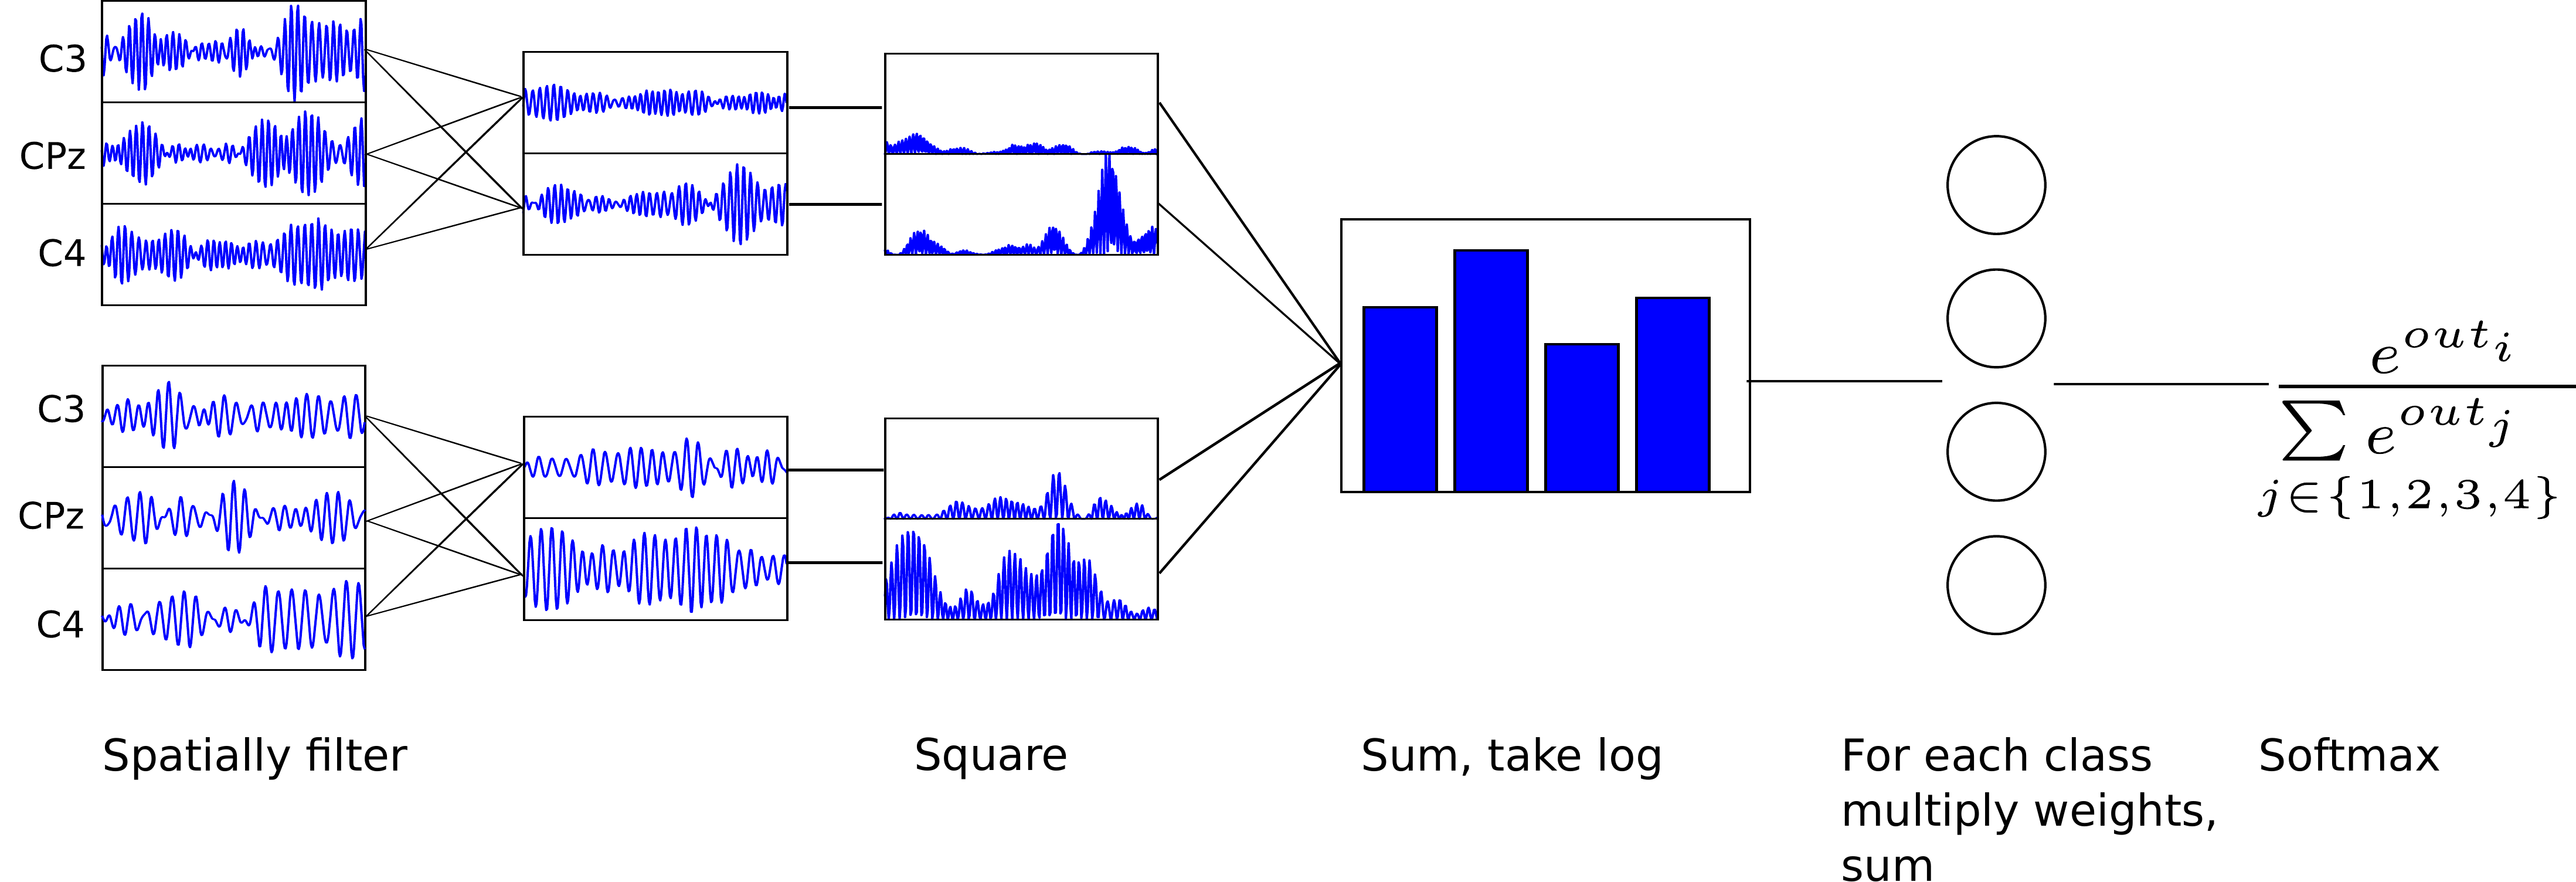
\includegraphics[width=1\linewidth]{images/csp_as_a_net_explanation.png}
    \caption[Filter bank network architecture overview.]{
\textbf{Filter bank network architecture overview.} Input signals were
bandpass filtered to different frequency ranges. Signals are first
transformed by learned spatial filters, then squared, summed and the
log-transformed. The resulting features are transformed into class
probabilities by a classification weights followed by the softmax
function. Figure taken from a master thesis
\citep{schirrmeister_msc_thesis_2015}.}\label{filterbank-net-figure}
\end{figure}


    The first neural network architecture was developed by us in a prior
master thesis \citep{schirrmeister_msc_thesis_2015} to
jointly learn the same steps that are learned separately by FBCSP (see
\Cref{filterbank-net-figure}). Concretely, the network
simultaneously learn the spatial filters across many frequency bands and
the classification weights for the log squared sums of all resulting
spatially filtered signals. To be able to do that, the network is fed
with input EEG signals that were bandpass-filtered to different
frequency ranges. The network then performs the following steps:




\begin{align*}
    \intertext{\textbf{Spatial Filtering}}
    h_1 &= W_s^Tx && \color{commentcolor}{\small \text{Apply spatial filter weights } W_s \text{ to  inputs }} \\
    \intertext{\textbf{Feature Construction}}
    h_2 &= h_1^2 && \color{commentcolor}{\small \text{Square the spatially filtered signals }} \\
    h_3 &=\sum_t (h_2) && \color{commentcolor}{\small \text{Sum the squared signals across trial timepoints } t} \\
    h_4 &= \log(h_3) && \color{commentcolor}{\small\text{Take the logarithm of the summed values}}\\
    \intertext{\textbf{Classification}}
    h_5 &= W_c^Th_4 && \color{commentcolor}{\small \text{Apply classifier weights } W_c \text{ on these features }} \\
    p(c_i|h_5) &= \frac{e^{h_{5,i}}}{\sum_j e^h_{5,j}} && \color{commentcolor}{\small \text{Take the softmax to compute class probabilities}} \\
\end{align*}

    The spatial filter weights and the classification weights are trained
jointly.

\todotext{textbox}

 

 %************************************************
\chapter{Cropped Training}\label{cropped-training}
%**************************************

\begin{startbox}{Cropped training means training on many temporal windows within one input example}  
\item Greatly increases the number of training examples
\item Can be made computationally efficient by avoiding redundant computations
\end{startbox}


    In this chapter, we describe a training strategy called ``cropped
training'' which addresses the problem of the relatively low number of
training examples in typical EEG datasets. The goal of this strategy is
to improve the performance of deep networks by training them on many
sliding temporal windows within the data. This approach had been
similarly used as spatial cropping in computer vision, where networks
are trained on multiple cropped versions of images. We first describe
the concept of regular, non-cropped training and then introduce cropped
training on a conceptual level. Finally, we discuss how to implement
this approach efficiently. Our aim is to demonstrate the effectiveness
and computational efficiency of cropped training as a regularization
technique for deep networks on EEG data.

Cropped training for EEG decoding was developed by me in the context of
this thesis. Some text and figures are adapted from from
\cite{schirrmeisterdeephbm2017}.


\section{Non-Cropped/Trialwise
Training}\label{non-croppedtrialwise-training}



\begin{figure}[bth]
    \myfloatalign
    \subfloat[\textbf{Trialwise training.} An entire single trial is fed
through the network and the network's prediction is compared to the
trial target to train the network.]
    {\label{trialwise-figure}
    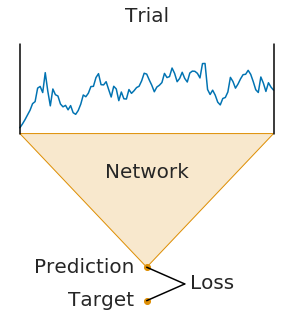
\includegraphics[width=.4\linewidth]{images/trialwise_explanation.png}} \quad
    \subfloat[\textbf{Cropped training.} A compute window contains many
temporal windows (crops) inside that are used as individual examples to
train the network.]
    {\label{cropped-figure}%
        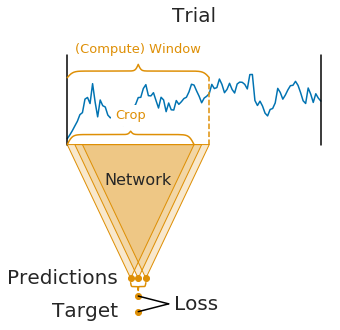
\includegraphics[width=.464\linewidth]{images/cropped_explanation.png}} 
    \caption[Trialwise and cropped training]{\textbf{Trialwise and cropped training.}}\label{cropped-and-trialwise-figure}
\end{figure}


In the trialwise training of neural networks on EEG data, each example
consists of the EEG signals from a single trial and its corresponding
label (see \Cref{trialwise-figure}). This might for example be a 4-second-trial where a subject moved
the left hand, with the 4-second-signal as the input and the left hand
as a label. Due to the typically small size of EEG datasets, networks
trained in this way may only be trained on a few hundred to a few
thousand examples per subject. This is significantly fewer examples than
those used to train networks in computer vision, where tens of thousands
or even millions of images are commonly used.


\section{Cropped Training}\label{cropped-training-section}

Cropped training increases the number of training examples by training
on many crops, i.e., temporal windows, within the trial (see \Cref{cropped-figure}). For example, in
a 4-second trial, all possible 2-second windows within the trial could
be used as ``independent'' examples. This approach drastically increases
the number of training examples, although many of the examples are
highly overlapping. This can be seen as an extreme version of using
random crops of images which is a method used to train deep networks in
computer vision. A naive implementation of cropped training would
greatly increase the computational cost per epoch due to the highly
increased number of examples. Thankfully, the high overlap between
neighbouring crops can be exploited for a more efficient implementation.



\section{Computationally Faster Cropped
Training}\label{computationally-faster-cropped-training}


\begin{figure}[ht]
    \myfloatalign
    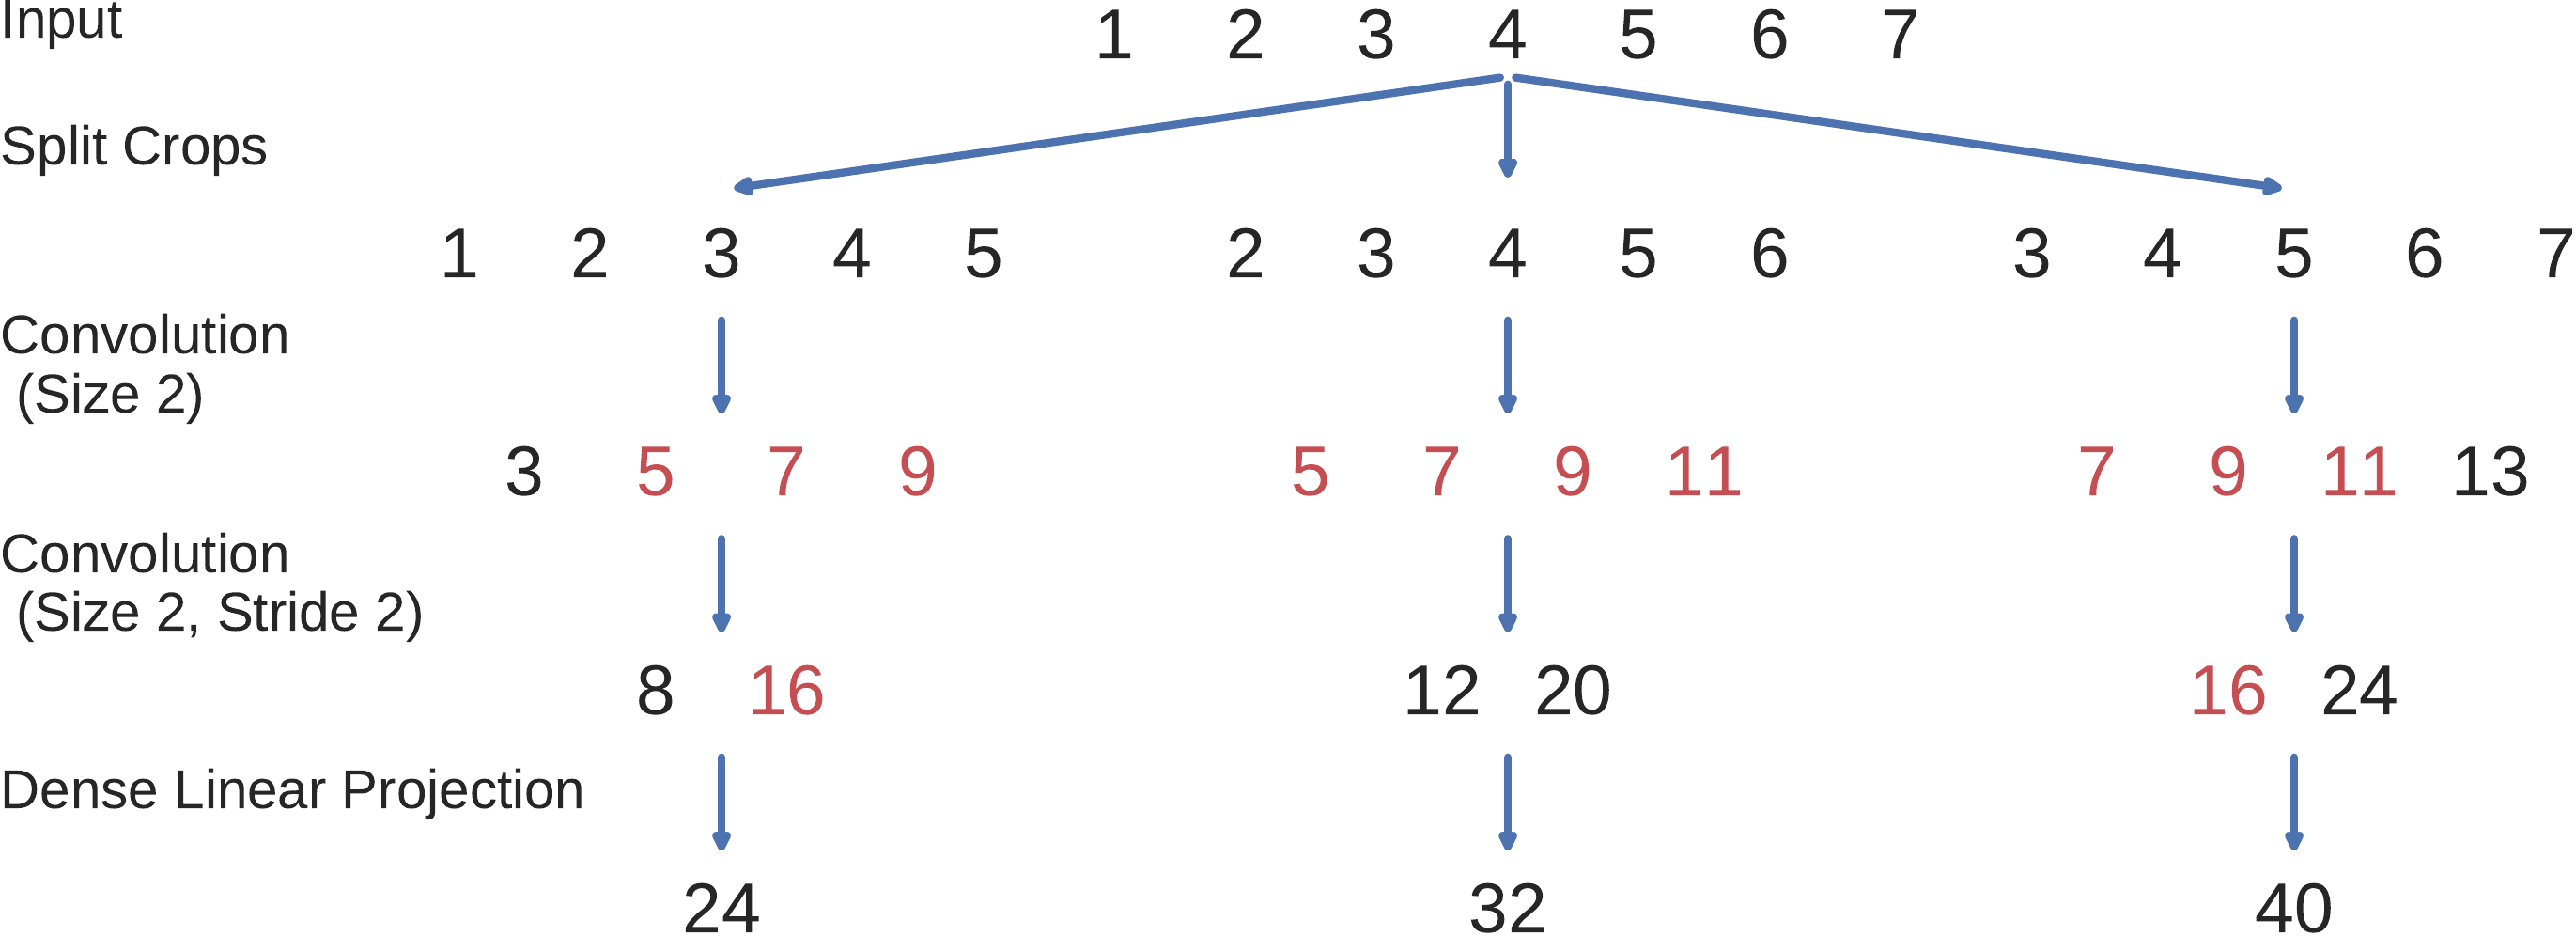
\includegraphics[width=1\linewidth]{images/Multiple_Prediction_Matplotlib_Graphics.ipynb.2.png}
    \caption[Naive cropped training toy example]{
\textbf{Naive cropped training toy example.} Each possible length-5 crop
is taken from the original length-7 trial and independently processed by
the Conv-Conv-Linear projection network. All filter values of the
network are assumed to be ones. Each crop is processed independently.
The values in red are identical and unnecessarily computed independently
for each crop. Figure from \cite{schirrmeisterdeephbm2017}.
}
\label{cropped-naive-computation-figure}
\end{figure}


\begin{figure}[ht]
    \myfloatalign
    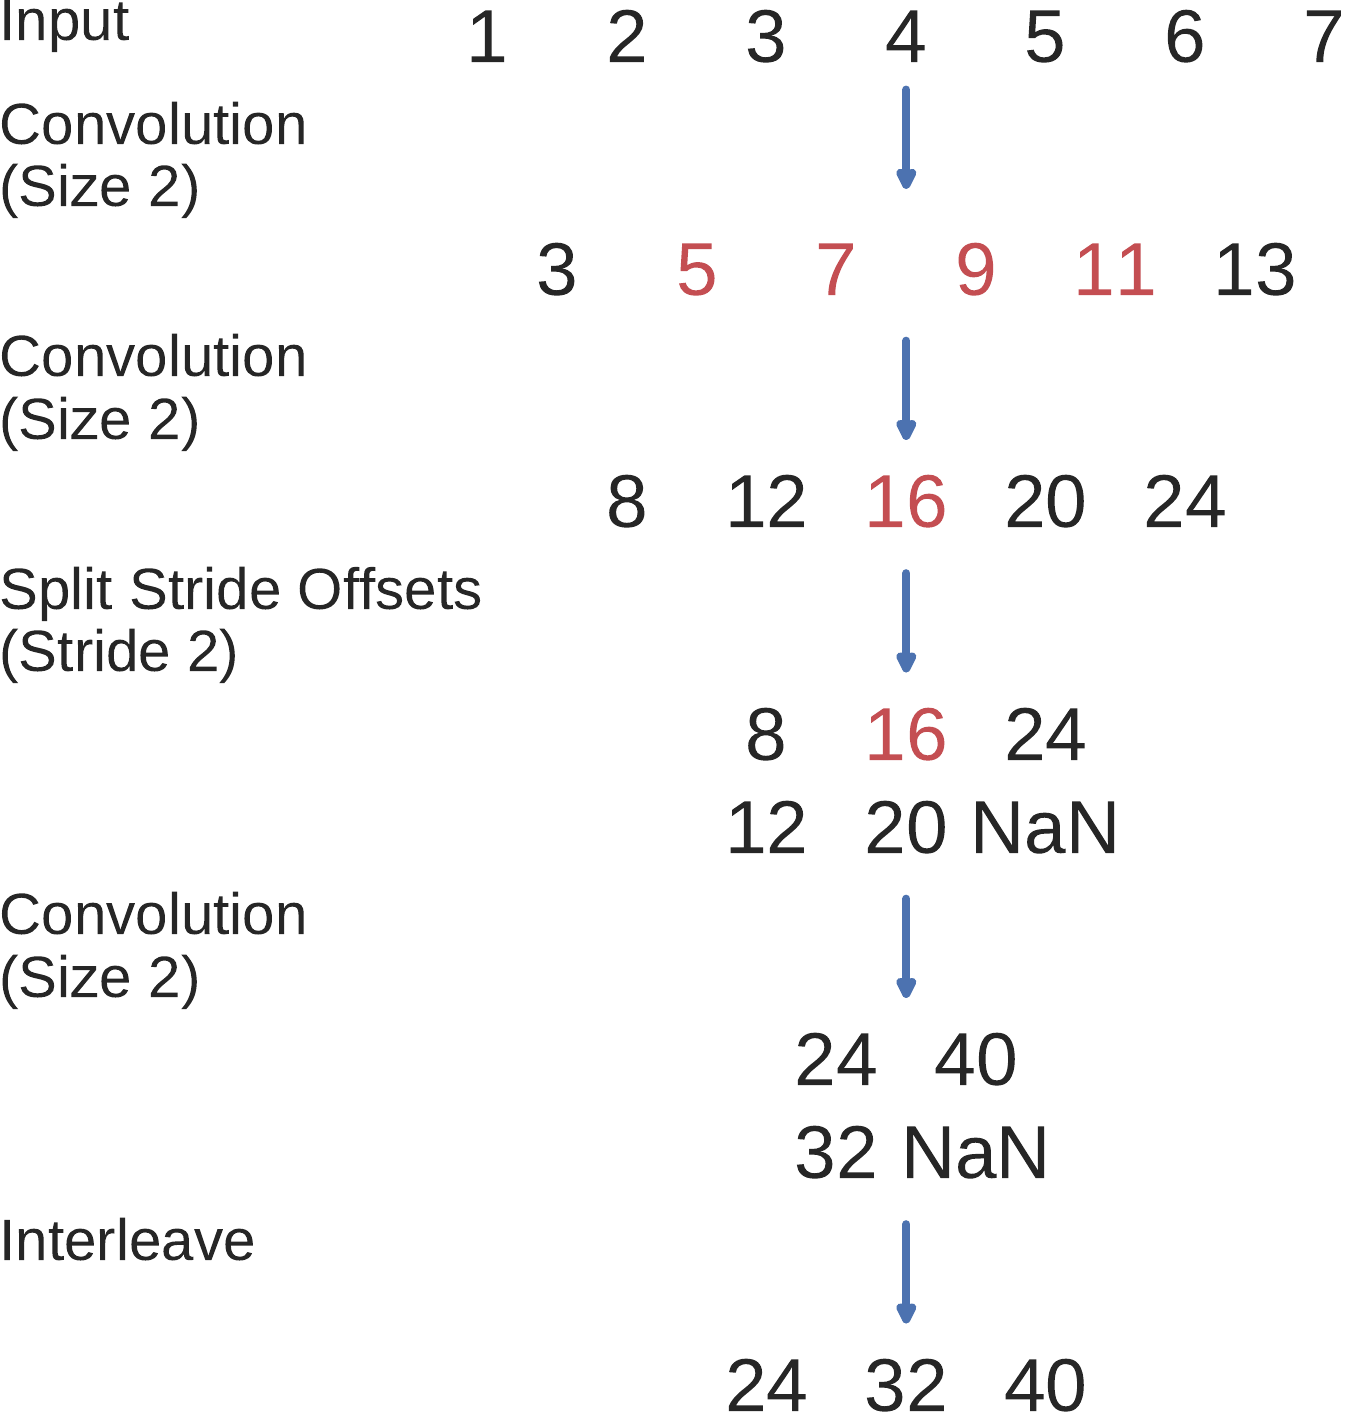
\includegraphics[width=0.5\linewidth]{images/Multiple_Prediction_Matplotlib_Graphics.ipynb.3.png}
    \caption[Efficient cropped training]{
    \textbf{Efficient cropped training.} Each possible length-5 crop is
    taken from the original length-7 trial and processed simultaneously by
    the Conv-Conv-Linear projection network, whilce still yielding the same
    results as if processed independently
    (\Cref{cropped-efficient-computation-figure}). All filter
    values of the network are assumed to be ones. Figure from
    \cite{schirrmeisterdeephbm2017}.
}
\label{cropped-efficient-computation-figure}
\end{figure}


    Cropped training can be implemented with substantially less computations
by exploiting that highly overlapping crops result in highly overlapping
intermediate network activations. By passing a group of neighbouring
crops together to the network, we can reuse intermediate computations.
See \Cref{cropped-naive-computation-figure} and
\Cref{cropped-efficient-computation-figure} for a concrete
example of this speedup method. This idea had been used in the same way
for dense predictions on images, e.g., for segmentation
\citep{giusti_fast_2013,nasse_face_2009,sermanet_overfeat:_2013,shelhamer_fully_2016}.

    Efficient cropped training then results in the exact same predictions
and training as if the neighbouring crops were passed separately through
the network. This is only true for networks that either use left-padding
or no padding at all to the input and the intermediate activations. In
the deep and shallow network described here, we do not use any padding.
In the residual network, we use padding, hence the training is not
exactly identical to passing neighbouring crops separately, but we still
found it to improve over trial-wise training.

    The more efficient way to do cropped training introduces a new
hyperparameter, the number of neighbouring crops that are decoded
together. The larger this hyperparameter, the more computations are
saved and the more speedup one gets (see
\citet{giusti_fast_2013} for a more detailed speedup analysis
on images). Larger numbers of neighbouring crops to simultaneously train
on require more memory and may also affect the training dynamics due to
more neighbouring crops being in the same mini-batch. However, we did
not find negative effects on the training dynamics from larger number of
simultaneously decoded neighbouring crops, consistent with prior work in
computer vision \citep{shelhamer_fully_2016}.

\begin{openbox}
\item For which datasets and architectures does cropped training help or hurt? 
\end{openbox}

%************************************************
\chapter{Perturbation Visualization}\label{perturbation-visualization}
%**************************************

\begin{startbox}{Perturbation visualization perturbs spectral features and measures change in classification predictions}
\item Can be used to investigate well-known spectral power features
\item Can also be implemented through gradients of spectral power features
\item Can be extended to investigate phase features
\end{startbox}


    What features the EEG-decoding ConvNet learns is a scientifically
interesting question and not straightforward to answer. Through
end-to-end training, the networks may learn a variety of features,
including brain-signal features and non-brain-signal features, e.g., eye
movements that correlate to a hand movement. The learned features may be
already known from prior research on brain-signal decoding or represent
novel features that had not been described in the literature. However,
there is no straightforward way to find out what the deep networks have
learned from the brain signals.

    Therefore, we developed an input amplitude perturbation method to
investigate whether the deep networks learn to extract spectral
amplitude features, which are very commonly used in many EEG decoding
pipelines. For example, it is known that the amplitudes, for example of
the alpha, beta and gamma bands, provide class-discriminative
information for motor tasks
\citep{ball_movement_2008,pfurtscheller_evaluation_1979,pfurtscheller_central_1981}.
Hence, it seems a priori very likely that the deep networks learn to
extract such features and worthwhile to check whether they indeed do so.
We also extended this method to investigate the use of phase information
by the networks.

The amplitude perturbation method was developed by me in the context of
this thesis, the phase perturbation method was developed by Kay Hartmann
together with me. Text and figures in this chapter are adapted from
\citep{schirrmeisterdeephbm2017} and \citep{hartmann2018hierarchical}.



\section{Input-Perturbation Network-Prediction Correlation
Map}\label{input-perturbation-network-prediction-correlation-map}


\begin{figure}[h!tb]
    \myfloatalign
    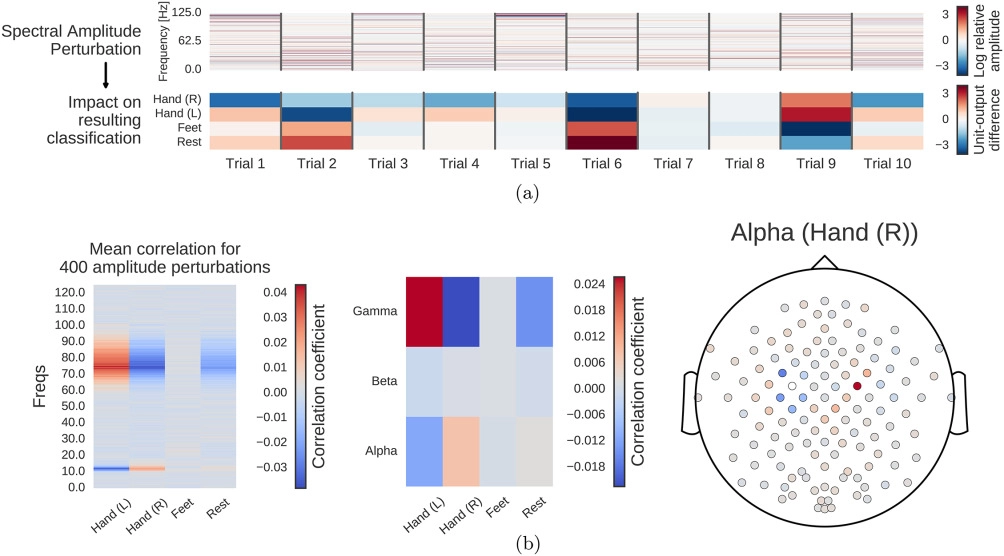
\includegraphics[width=1\linewidth]{images/input-perturbation-overview.png}
    \caption[Computation overview amplitude perturbation]{

\textbf{Computation overview for input-perturbation network-prediction
correlation map.} (a) Example spectral amplitude perturbation and
resulting classification difference. Top: Spectral amplitude
perturbation as used to perturb the trials. Bottom: unit-output
difference between unperturbed and perturbed trials for the
classification layer units before the softmax. (b) Input-perturbation
network-prediction correlations and corresponding network correlation
scalp map for alpha band. Left: Correlation coefficients between
spectral amplitude perturbations for all frequency bins and differences
of the unit outputs for the four classes (differences between
unperturbed and perturbed trials) for one electrode. Middle: Mean of the
correlation coefficients over the the alpha (7--13 Hz), beta (13--31 Hz)
and gamma (71--91 Hz) frequency ranges. Right: An exemplary scalp map
for the alpha band, where the color of each dot encodes the correlation
of amplitude changes at that electrode and the corresponding prediction
changes of the ConvNet. Negative correlations on the left sensorimotor
hand/arm areas show an amplitude decrease in these areas leads to a
prediction increase for the Hand (R) class, whereas positive
correlations on the right sensorimotor hand/arm areas show an amplitude
decrease leads to a prediction decrease for the Hand (R) class. Figure
from \cite{schirrmeisterdeephbm2017}.
}
\label{input-perturbation-overview-figure}
\end{figure}

    To investigate the causal effect of changes in power on the deep
ConvNet, we correlated changes in ConvNet predictions with changes in
amplitudes by perturbing the original trial amplitudes (see
\Cref{input-perturbation-overview-figure} for an overview).
Concretely, the visualization method performs the following steps: 

\begin{enumerate}
\item
Transform all training trials into the frequency domain by a Fourier
transformation 
\item
Randomly perturb the amplitudes by adding Gaussian
noise (with mean 0 and variance 1) to them (phases were kept
unperturbed) 
\item
Retransform perturbed trials to the time domain by the
inverse Fourier transformation
\item
Compute predictions of the deep
ConvNet for these trials before and after the perturbation (predictions
here refers to outputs of the ConvNet directly before the softmax
activation)
\item
Repeat this procedure with 400 perturbations sampled from
aforementioned Gaussian distribution
\item
Correlate the change in input
amplitudes (i.e., the perturbation/noise we added) with the change in
the ConvNet predictions.
\end{enumerate}


To ensure that the effects of our perturbations reflect the behavior of
the ConvNet on realistic data, we also checked that the perturbed input
does not cause the ConvNet to misclassify the trials (as can easily
happen even from small perturbations, see
\citep{szegedy_intriguing_2014}. For that, we computed
accuracies on the perturbed trials. For all perturbations of the
training sets of all subjects, accuracies stayed above 99.5\% of the
accuracies achieved with the unperturbed data.

This method can not only be applied to final predictions, but also to
investigate any intermediate network filter's activations in order to
better understand the intermediate computations of the network.


\section{Gradient-Based
Implementation}\label{gradient-based-implementation}

    A simpler and more computationally efficient way to implement the idea
of testing the sensitivity of the network to spectral amplitude features
is through gradient-based analysis \footnote{This idea was suggested to
  us in personal communication by Klaus-Robert Müller.}. There, we
directly compute the gradient of the output unit with respect to the
amplitudes of all frequency bins of all electrodes of the original
unperturbed trial. To practically implement this, one must first
transform the time domain input signal into the frequency domain and to
a amplitude/phase representation via the Fourier transform. Then, one
can transform the amplitude/phase representation back to the time domain
using the inverse Fourier Transform. Since the inverse Fourier transform
is differentiable, one can backpropagate the gradients from the output
unit through the time domain input back to the amplitudes. The more the
network behaves locally linear around the input, the closer the results
of this variant would be to the original perturbation variant. It is
computationally substantially faster as the gradient is computed in one
forward-backward pass, without needing to iterate over many
perturbations. The gradient-based method may produce less insightful
visualizations for a given input example if the prediction function of the network is locally very nonlinear but has an approximately linear relationship
with the spectral amplitudes in a larger neighbourhood around the input example. See works on other saliency/gradient-based visualizations for
discussions in this topic,
e.g. ~\citet{sturmfels2020visualizing}.


\section{Extension to Phase-Based
Perturbations}\label{extension-to-phase-based-perturbations}

\begin{figure}[h!tb]
    \centering
    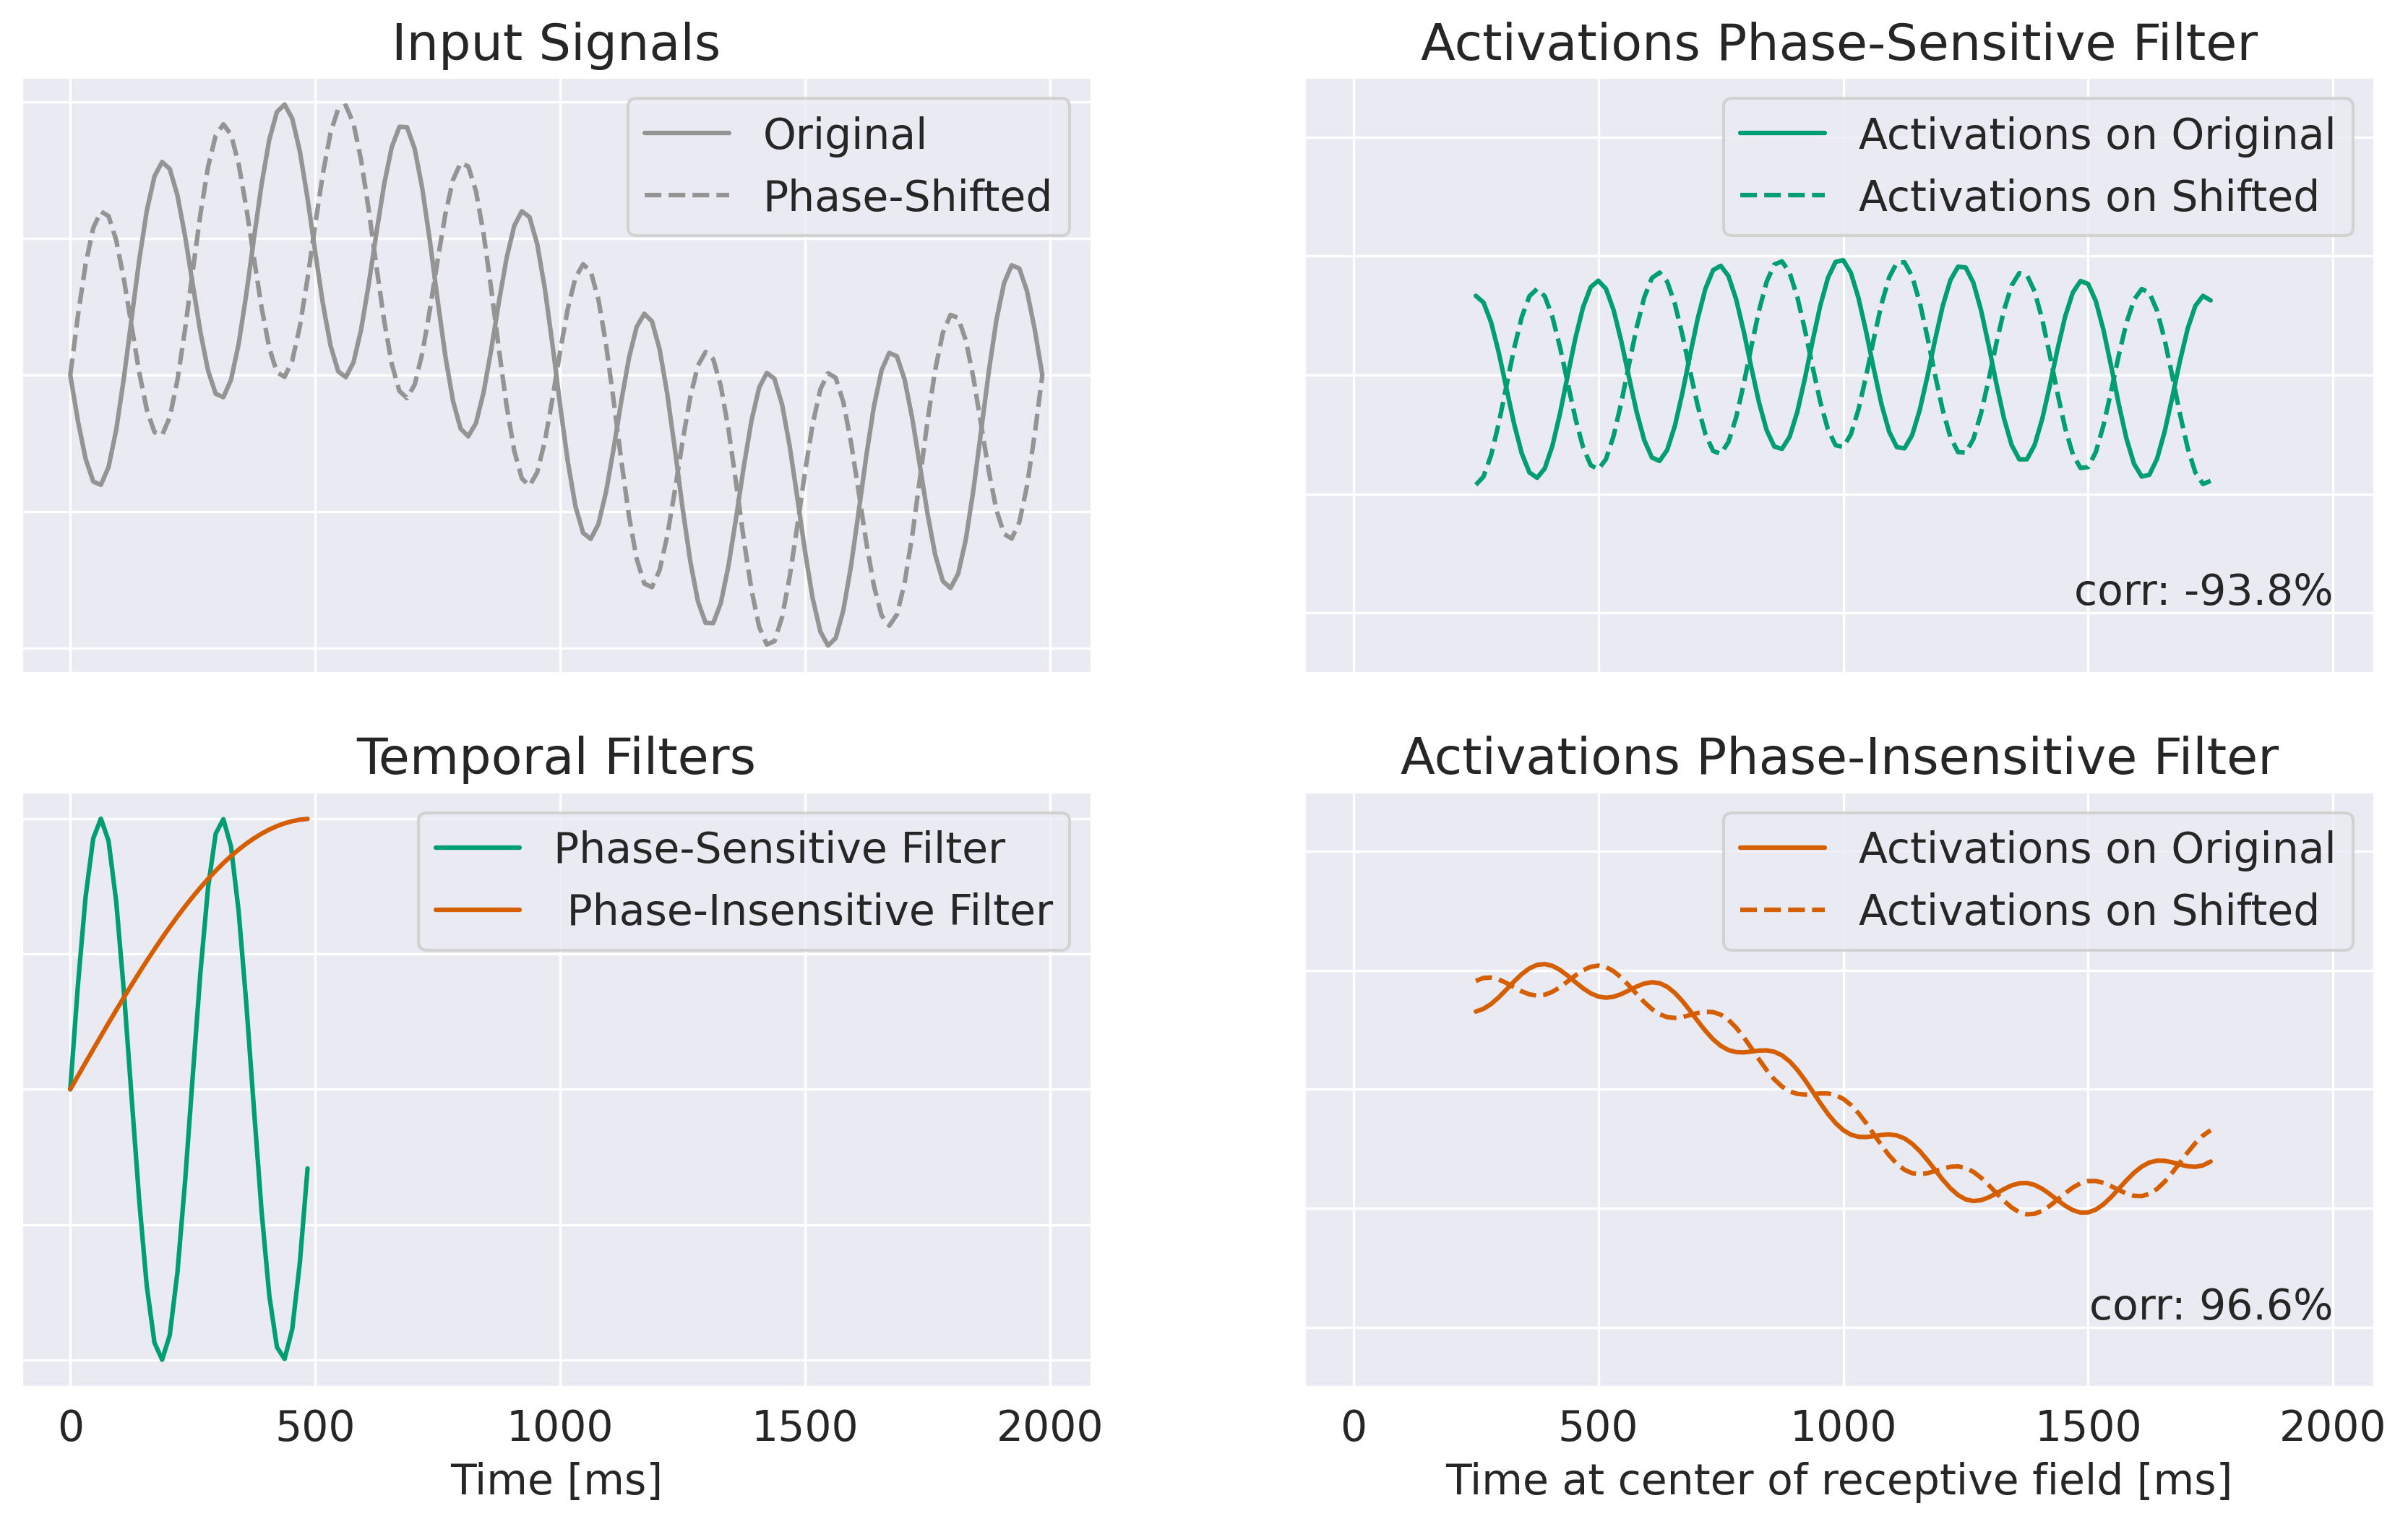
\includegraphics[width=.75\linewidth]{images/phase-perturbation-corr.png}
    \caption[Phase perturbation intuition]{

\textbf{Intuition of the phase perturbation
correlation method.} Top left: two input signals
where the phase of one frequency has been shifted between the two
signals. Bottom left: two temporal filters, one phase-sensitive
and one phase-insensitive to the frequency where the phase was shifted.
Right: activations for the phase-sensitive and
phase-insensitive filter for the original and the shifted signal. The correlation between activations of the phase-sensitive filter is
very low, even negative (-93.8\%), whereas correlation between the
activations of the phase-insensitive filter remains high at 96.6\%. Note
that this simplified example does not illustrate some key mechanisms for
activations to become more generally phase-insensitive such as
nonlinearities and pooling operations.
}
\label{phase-perturbation-corr-figure}
\end{figure}


    The amplitude-perturbation method can be extended to investigate in
the use of phase features by the networks´. The response
of filters to changes in the phase of certain frequencies was calculated
similarly to the amplitude perturbation correlations. However, because
of the cyclic nature of phase features, the change of activations in a
filter resulting from a phase shift cannot be quantified using the mean
activation difference. When you change the phase of the frequency that a
filter is sensitive to, you won't expect the activations of the filter
to increase uniformly throughout the window. Instead, the activations of
a phase-sensitive filter will probably be temporally shifted by the
phase change. Units of filters whose receptive field contained its
specific phase in the original signal should activate less and units
whose receptive field contains the specific phase in the perturbed
signal should then activate more. Therefore, the original activations
and the activations on the perturbed input should have a decreased
correlation (less than 1). Activation and correlation should remain
similar for phase-insensitive filters. See also \Cref{phase-perturbation-corr-figure} for an illustration.

Phase perturbations were sampled from $p^{P}_{\xi,i}{\sim}N(0,\pi)$.
Perturbed phases $P^{P}_\xi$ were calculated by shifting the phase:
$P^{P}_\xi(X_i)=p^{P}_{\xi,i}+P_\xi(X_i)$. Perturbed signals $X^{P}$
were reconstructed by inverse Fourier transformation. The correlation
between original and perturbation filter activations of a filter $f$
from trial $i$ is denoted by
$\rho_{y_{f,i},y^{P}_{f,i}}=corr(y_{f,i},y^{P}_{f,i})$. Correlations
between phase perturbations $p^{P}_{\xi}$ and filter activity
correlations $\rho_{y_{f},y^{P}_{f}}$ were calculated identically to
amplitude perturbations. The resulting mean absolute phase perturbation
correlations for each layer is denoted as $\varrho^P_{l,\xi}$.

Since we wanted to study only the effect of changing the overall phase
of the signal, independent of the effect of increased or decreased phase
synchronicity across EEG channels, we did not perturb the phase in
channels individually, but applied one phase perturbation of a certain
frequency in all channels equally.

\section{Interpretation and Limitations}
\label{perturbation-visualization-interpretation}


    The perturbation-based visualization reflects network behavior and one
cannot directly draw inferences about the data-generating process from
it. This is because a prediction change caused by an amplitude
perturbation may reflect both learned task-relevant factors as well as
learned noise correlations. For example, increasing the alpha-band
amplitude at electrode C4 (located on the right side), may increase the
predicted probability for right hand movement. That would likely not be
because the alpha amplitude actually increases at C4 during right hand
movement, but because the amplitude \emph{decreases} on C3 \emph{and} is
correlated between C3 and C4. Hence, first subtracting the C4 amplitude
from the C3 amplitude and then decoding associating negative values of
this computation with right hand movement is a reasonable learned
prediction function. And this learned prediction function would cause
the amplitude-perturbation function to show that an alpha increase at C4
causes an increase in the predicted probability for right hand movement.
For a more detailed discussion of this effect in the context of linear
models, see \citep{haufe_interpretation_2014}.

\begin{openbox}
\item Do spectral maps obtained from this visualization show neurophysiologically plausible patterns?
\item What can they reveal about the inner computations of the networks?
\end{openbox}

    


%************************************************
\chapter{Invertible Networks}\label{invertible-networks}
%**************************************

\begin{startbox}{Invertible networks can help understand learned discriminative features in the EEG}
\item Class prototypes can be visualized
\item Per-electrode prototypes may be even more interpretable
\item Additionally, a small interpretable network may allow further insights
\end{startbox}


Invertible networks are networks that are invertible by design, i.e.,
any network output can be mapped back to a corresponding input
bijectively \citep{DBLP:journals/corr/DinhKB14,DBLP:journals/corr/DinhSB16,DBLP:conf/nips/KingmaD18,DBLP:conf/icml/RezendeM15,DBLP:conf/icml/HoCSDA19}.
The ability to invert any output back to the input enables different
interpretability methods and furthermore allows training invertible
networks as generative models via maximum likelihood.

This chapter starts by explaining invertible layers that are used to
design invertible networks, proceeds to detail training methodologies
for invertible networks as generative models or classifiers, and goes on
to outline interpretability techniques that help reveal the learned
features crucial for their classification tasks.

\section{Invertible Layers}\label{invertible-layers}

    Invertible networks use layers constructed specifically to maintain
invertibility, thereby rendering the entire network structure
invertible. Often-used invertible layers are coupling layers, invertible
linear layers and activation normalization layers
\citep{DBLP:conf/nips/KingmaD18}.

\textbf{Coupling layers} split a multidimensional input $x$ into two
parts $x_1$ and $x_2$ with disjoint dimensions and then use $x_2$
to compute an invertible transformation for $x_1$. Concretely, for an
additive coupling layer, the forward computation is:


\begin{align*}
    y_1 &= x_1 + f(x_2) && \codecomment{\text{Compute } y_1 \text{ from } x_1 \text{ and arbitrary function f of } x_2} \\
    y_2 &= x_2 && \codecomment{\text{Leave } x_2 \text{ unchanged}} \\
\intertext{The inverse computation is:}
    x_1 &= y_1 - f(y_2) && \codecomment{\text{Invert to } x_1 \text{ using unchanged } y_2=x_2} \\
    x_2 &= y_2 &&  \codecomment{x_2 \text{ was unchanged}}\\
\end{align*}

% 

For the splitting of the dimensions in a timeseries, there are multiple
ways, such as using the even time indices as $x_1$ and all the odd
time indices as $x_2$ or using difference and mean between two
neighbouring samples (akin to one stage of a Haar Wavelet). The function
$f$ is usually implemented by a neural network, in our cases it will
be small convolutional networks. Instead of addition any other
invertible function can be used, affine transformation are commonly
used, where $f$ produces translation and scaling coefficients $f_t$
and $f_s$:
\begin{align*}
    y_1 &= x_1 \cdot f_s(x_2) + f_t(x_2) && \text{ } y_2=x_2 && \codecomment{\text{Affine Forward }} \\
    \\
    x_1 &= \frac{(y_1  - f_t(y_2))}{f_s(y_2)} && \text{ } x_2=y_2 && \codecomment{\text{Affine Inverse}} \\
\end{align*}

\textbf{Invertible linear layers} compute an invertible linear
transformation (an automorphism) of their input. Concretely they
multiply a $d$-dimensional vector $\mathbf{x}$ with a
$dxd$-dimensional matrix $W$, where $W$ has to be invertible,
i.e., have nonzero determinant.

\begin{align*}
    y&=W \mathbf{x} && \codecomment{\text{Linear Forward }} \\
    x&=W^{-1} \mathbf{y} && \codecomment{\text{Linear Inverse}} \\
\end{align*}

For multidimensional arrays like feature maps in a convolutional
network, these linear transformations are usually done per-position, as
so-called invertible 1x1 convolutions in the 2d case.


\textbf{Activation normalization layers} perform an affine
transformation with learned parameters with $s$ and $t$ learned
scaling and translation parameters (independent of the input $x$):

\begin{align*}
    y&=x \cdot{s} + t && \codecomment{\text{ActNorm Forward}} \\
    x&=\frac{y - t}{s} && \codecomment{\text{ActNorm Inverse}} \\
\end{align*}

These have also been used to replace batch normalization and are often
initialized data-dependently to have standard-normalized activations at
the beginning of training.


\section{Generative Models by Maximizing Average Log
Likelihood}\label{generative-models-by-maximizing-average-log-likelihood}

    Invertible networks can also be trained as generative models via
maximizing the average log likelihood. In this training, the network is
optimized to maximize the average log probabilities of the training
inputs, which is equivalent to minimizing the Kullback-Leibler (KL)
divergence between the training distribution and the learned model
distribution \cite{DBLP:journals/corr/TheisOB15}. Invertible
networks assign probabilities to training inputs $x$ by mapping them
to a latent space $z=f(x)$ and computing their probabilities under a
predefined prior $p_z(z)$ in that latent space. For real-valued
inputs, one has to account for quantization and volume change to ensure
this results in a proper probability distribution $p_x$ in the input
space. Quantization refers to the fact that training data often consists
of quantized measurements of underlying continuous data, e.g.~digital
images can only represent a distinct set of color values. Volume change
refers to how the invertible networks' mapping function $f$ expands or
squeezes volume from input space to latent space.

\subsection{(De)quantization}\label{dequantization}
    
\begin{figure}[ht]
    \myfloatalign
    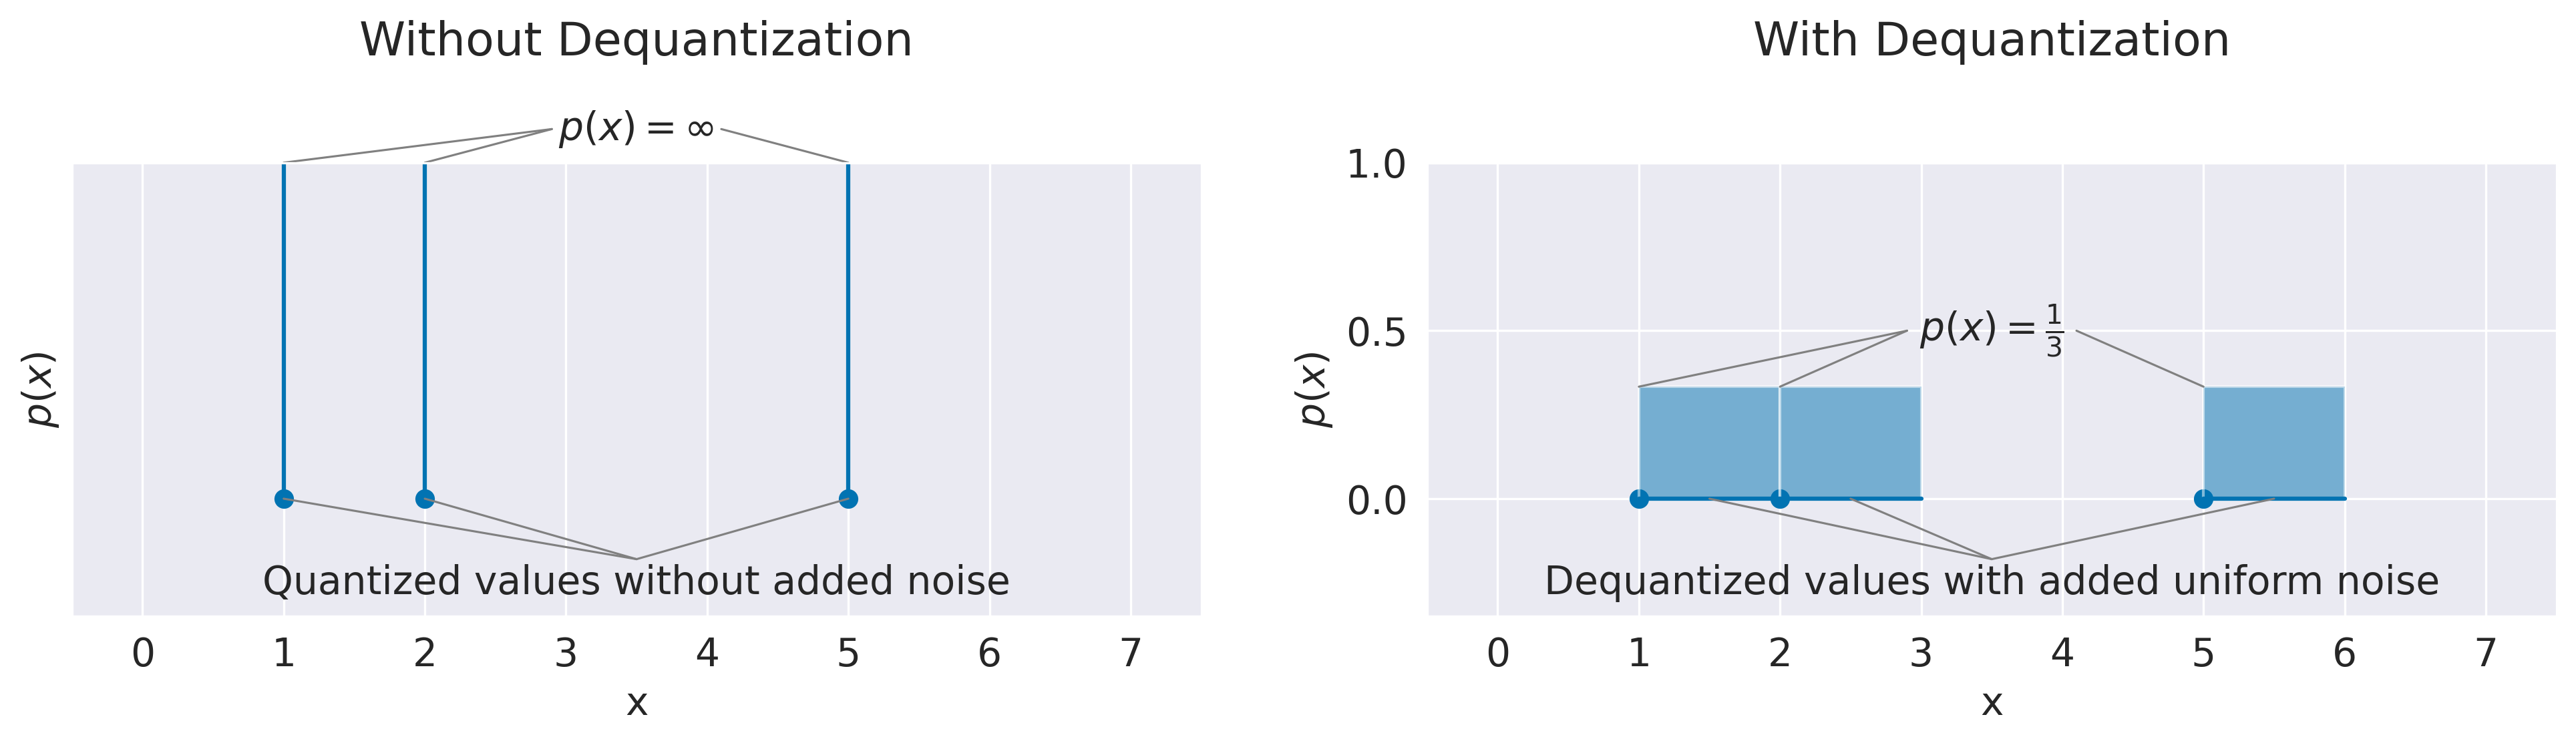
\includegraphics[width=1\linewidth]{images/dequantization.png}
    \caption[Average log-likelihood-maximizing distributions without and with
dequantization]{
\textbf{Average log-likelihood-maximizing distributions without and with
dequantization.} Examples show result of fitting quantized values like
discrete integer color values with a continuous probability
distribution. Example training distributions have 3 data points at
$x_1=1$, $x_2=2$ and $x_3=5$. On the left, fitting quantized
values directly leads to a pathological solution as the learned
distribution $p$ can assign arbitrarily high probability densities on
the data points. On the right, adding uniform noise $U(0,1)$ to the
datapoints leads to a distribution that also recovers the correct
discrete distribution, that means integrating over the probability
densities in the volume of each point leads to $P(x_i)=\frac{1}{3}$.
}
\label{dequantization-fig}
\end{figure}

    

    Often, training data for neural networks consists of quantized
measurements like discrete integer color values from 0 to 255, which are
mapped to real-world floating point numbers for training. Naively
maximizing the average log probability densities of these quantized
values with a continuous probability distribution would lead to
pathological behavior as the quantized training data points do not cover
any volume. Hence it would be possible for the learned distribution to
assign infinitely high probability densities to individual data points,
see \Cref{dequantization-fig} for an illustration.

Hence, one needs to ``dequantize'' the data such that each datapoint
occupies volume in the input space
\citep{DBLP:journals/corr/DinhSB16,DBLP:conf/icml/HoCSDA19}.
The simplest way here is to add uniform noise to each data point with a
volume corresponding to the gap between two data points. For example, if
the 256 color values are mapped to 256 floating values between 0 and 1,
one may add uniform noise $u\sim(0,\frac{1}{256})$ to the inputs. Then
the KL-divergence between the dequantized continuous distribution and
the learned continuous distribution is upper bounded by the
KL-divergence between the underlying discrete distribution and the
learned discrete distribution obtained by integrating over the noise
samples for each input \citep{DBLP:journals/corr/TheisOB15}.
Since in our case, we are not primarily interested in the exact
performance as a generative model in terms of number of bits, we simply
add gaussian noise with a fixed small standard deviation $N(0,0.005I)$
during training.

\subsection{Volume Change}\label{volume-change}

\begin{figure}[ht]
    \myfloatalign
    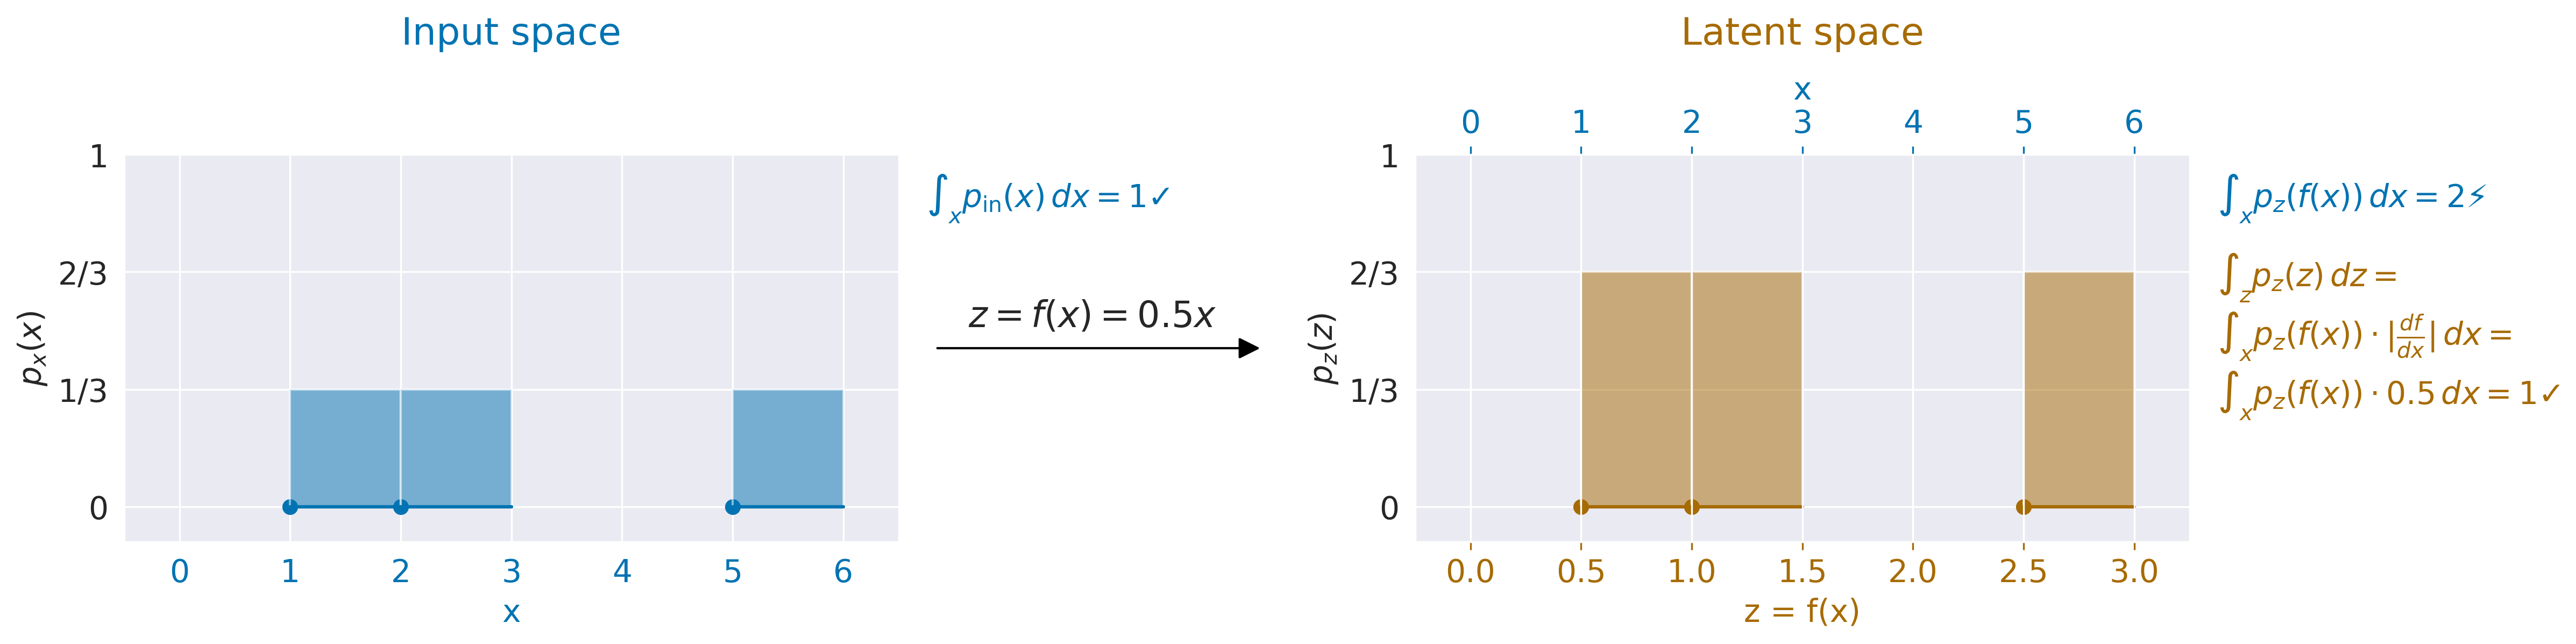
\includegraphics[width=1\linewidth]{images/change-of-volume.png}
    \caption[Volume change illustration]{
\textbf{Probability densities and volume changes.} Computing probability densities taking into account how a mapping function changes volume. Input $x$ with probability distribution $p_\text{x}(x)$
on the left is scaled by 0.5 to $z=f(x)=0.5x$ with probability
distribution $p_\text{z}(z)$ on the right. Naively integrating
$p_\text{z}(f(x))$ over x would lead to a non-valid probability
distribution with $\int_x p_\mathrm{z}(f(x)) \, dx=2$. To get the
prober probability densities in input space from $p_\text{z}(z)$, one
has to multiply with the volume changes, in this case the scaling factor
of the mapping $f(x)$ from x to z, giving
$p_\text{x}(x)=p_\mathrm{z}(f(x)) \cdot \frac{df}{dx}=p_\mathrm{z}(f(x))\cdot 0.5$
which correctly integrates to 1.
}
\label{change-of-volume-fig}
\end{figure}



    In addition, for these probability densities in latent space to form a
valid probability distribution in the input space, one has to account
for how much the network's mapping function squeezes and expands volume.
Otherwise, the network can increase densities by squeezing all the
inputs closely together in latent space, see also
\Cref{change-of-volume-fig} for a onedimensional example. To
correctly account for the volume change during the forward pass of $f$
one needs to multiply the probability density with the volume change of
$f$, descreasing the densities if the volume is squeezed from input to
latent space and increasing it if the volume is expanded. As the volume
change at a given point $x$ is given by the absolute determinant of
the jacobian of f at that point
$\det \left( \frac{\partial \mathbf{f}}{\partial \mathbf{x}} \right)$,
the overall formula looks like this:

\begin{align}
p(x) = p_\textrm{z}(f(x)) \cdot | \det \left( \frac{\partial \mathbf{f}}{\partial \mathbf{x}} \right)|
\end{align}

Or in log-densities:

\begin{align}
\log p(x) = \log p_\textrm{z}(f(x)) + \log |\det \left( \frac{\partial \mathbf{f}}{\partial \mathbf{x}} \right)|
\end{align}

\section{Generative Classifiers}\label{generative-classifiers}

    Invertible networks trained as class-conditional generative models can
also be used as classifiers. Class-conditional generative networks may
be implemented in different ways, for example with a separate prior in
latent space for each class. Given the class-conditional probability
densities $p(x|c_i)$, one can obtain class probabilities via Bayes'
theorem as $p(c_i|x)=\frac{p(x|c_i)}{\sum_jp(x|c_j)}$.

Pure class-conditional generative training may yield networks that
perform badly as classifiers. One proposed reason is the relatively
small reduction in optimal average log likelihood loss obtainable from
providing the class label to the network for high-dimensional inputs,
often much smaller than typical differences between two runs of the same
network \citep{DBLP:journals/corr/TheisOB15}. The reduction
in the optimal average log likelihood loss through providing the class
label can be derived from a compression perspective. According to
Shannon's theorem, more probable inputs need less bits to encode than
less probable inputs, or more precisely: 
$\textrm{Number of bits needed}(x) = \log_2 p(x)$. How many of these
bits are needed for the class label in case it is not given? To
distinguish between n classes, one needs only $\log_2(n)$ bits, so in
case of binary pathology classification, only 1 bit is needed. Therefore
the optimal class-conditional model will only be 1 bit better than the
optimal class-independent model. However, the inputs themselves
typically need at least 1 bit per dimension, so already, a 21 channel x
128 timepoints EEG-signal may need at least 2688 bits to encode. Hence,
the class encoding contributes very little to the overall encoding size
and maximum likelihood loss. In contrast, the loss difference between
two training runs of the same network will typically be at least one to
two orders of magnitude larger. Still, in practice, the gains from using
a class-conditional model, by e.g., using a separate prior per class in
latent space, are often larger, but it is not a priori clear if the
reductions in loss from exploiting the class label are high enough to
result in a good classification model.

Various methods have been proposed to improve the performance of using
generative classifiers. For example, people have fixed the per-class
latent gaussian priors so that they retain the same distance throughout
training \citep{DBLP:conf/icml/IzmailovKFW20} or added a
classification loss term
\begin{align*}
L_\textrm{class}(x,c_i)&=-\log p(c_i|x)\\
&= -\log \frac{p(x|ci)}{\sum_j p(x|cj)}\\
&=-\log \frac{e^{\log p(x|ci)}}{\sum_j e^{\log p(x|cj)}}\\
&=-\log \left( \mathrm{softmax}\left({\log p(x|c_i)}\right) \right)
\end{align*}

to the training loss\citep{DBLP:conf/nips/ArdizzoneMRK20}. In
our work, we experimented with adding a classification loss term to the
training, and also found using a learned temperature before the softmax
helps the training, so leading to:
\begin{equation}
\begin{split}
   L_\textrm{class}(x,c_i,t)&= -\log \frac{e^{\frac{\log p(x|ci)}{t}}}{\sum_j e^{\frac{\log p(x|cj)}{t}}}=-\log \left( \mathrm{softmax}\left({\frac{\log p(x|c_i)}{t}}\right) \right) \\
\end{split}
\end{equation}

Our overall training loss is simply a weighted sum of generative loss
and classification loss:

\begin{equation}
\begin{split}
   L(x,c_i,t)&= L_\textrm{class}(x,c_i,t) + L_\textrm{gen}(x,c_i)\\
   &= -\log \left( \mathrm{softmax}\left({\frac{\log p(x|c_i)}{t}}\right) \right) - \alpha \log p(x|ci)\\
\end{split}
\end{equation}


where we choose the hyperparameter $\alpha$ as the inverse of the
number of dimensions $\alpha=\frac{1}{\textrm{Number of dimensions of x}}$.

\section{Invertible Network for EEG
Decoding}\label{invertible-network-for-eeg-decoding}


\begin{figure}[htb]
    \myfloatalign
    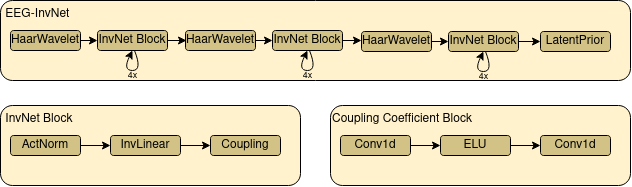
\includegraphics[width=1\linewidth]{images/EEG-InvNet.png}
    \caption[EEG-InvNet architecture]{
\textbf{EEG-InvNet architecture.} Our EEG-InvNet architecture consists
of three stages that operate at sequentially lower temporal resolutions.
Input is two seconds of 21 electrodes at 64 Hz so 21x128 dimensions.
These are downsampled using Haar Wavelets to 42x32 for the first, 84x16
for the second and 164x8 for the last stage. One stage consists of 4
blocks, each block has an activation normalization, an invertible linear
and a coupling layer. The activation normalization and invertible linear
layer act on the channel dimension, so perform the same operation across
channels on timepoint in the feature map. The coupling layer uses two
convolutions with an exponential linear unit activation inbetween.
}
\label{eeg-invnet-fig}
\end{figure}




    We designed an invertible network named EEG-InvNet for EEG Decoding
using invertible components used in the literature, primarily from the
Glow architecture \citep{DBLP:conf/nips/KingmaD18}. Our
architecture consists of three stages that operate on sequentially lower
temporal resolutions. Similar to Glow, the individual stages consists of
several blocks of Activation Normalization, Invertible Linear Channel
Transformations and Coupling Layers, see
\Cref{eeg-invnet-fig}. Between each stage, we downsample by
computing the mean and difference of two neighbouring timepoints and
moving these into the channel dimension. Unlike Glow, we keep processing
all dimensions throughout all stages, finding this architecture to reach
competitive accuracy on pathology decoding. We use one gaussian
distribution per class in the latent space. We experimented with affine
and additive coupling layers, and report results for additive layers as
the restricted expressiveness may make them easier to interpret.

\section{Class Prototypes}\label{methods-class-prototypes}


\begin{figure}[htb]
    \myfloatalign
    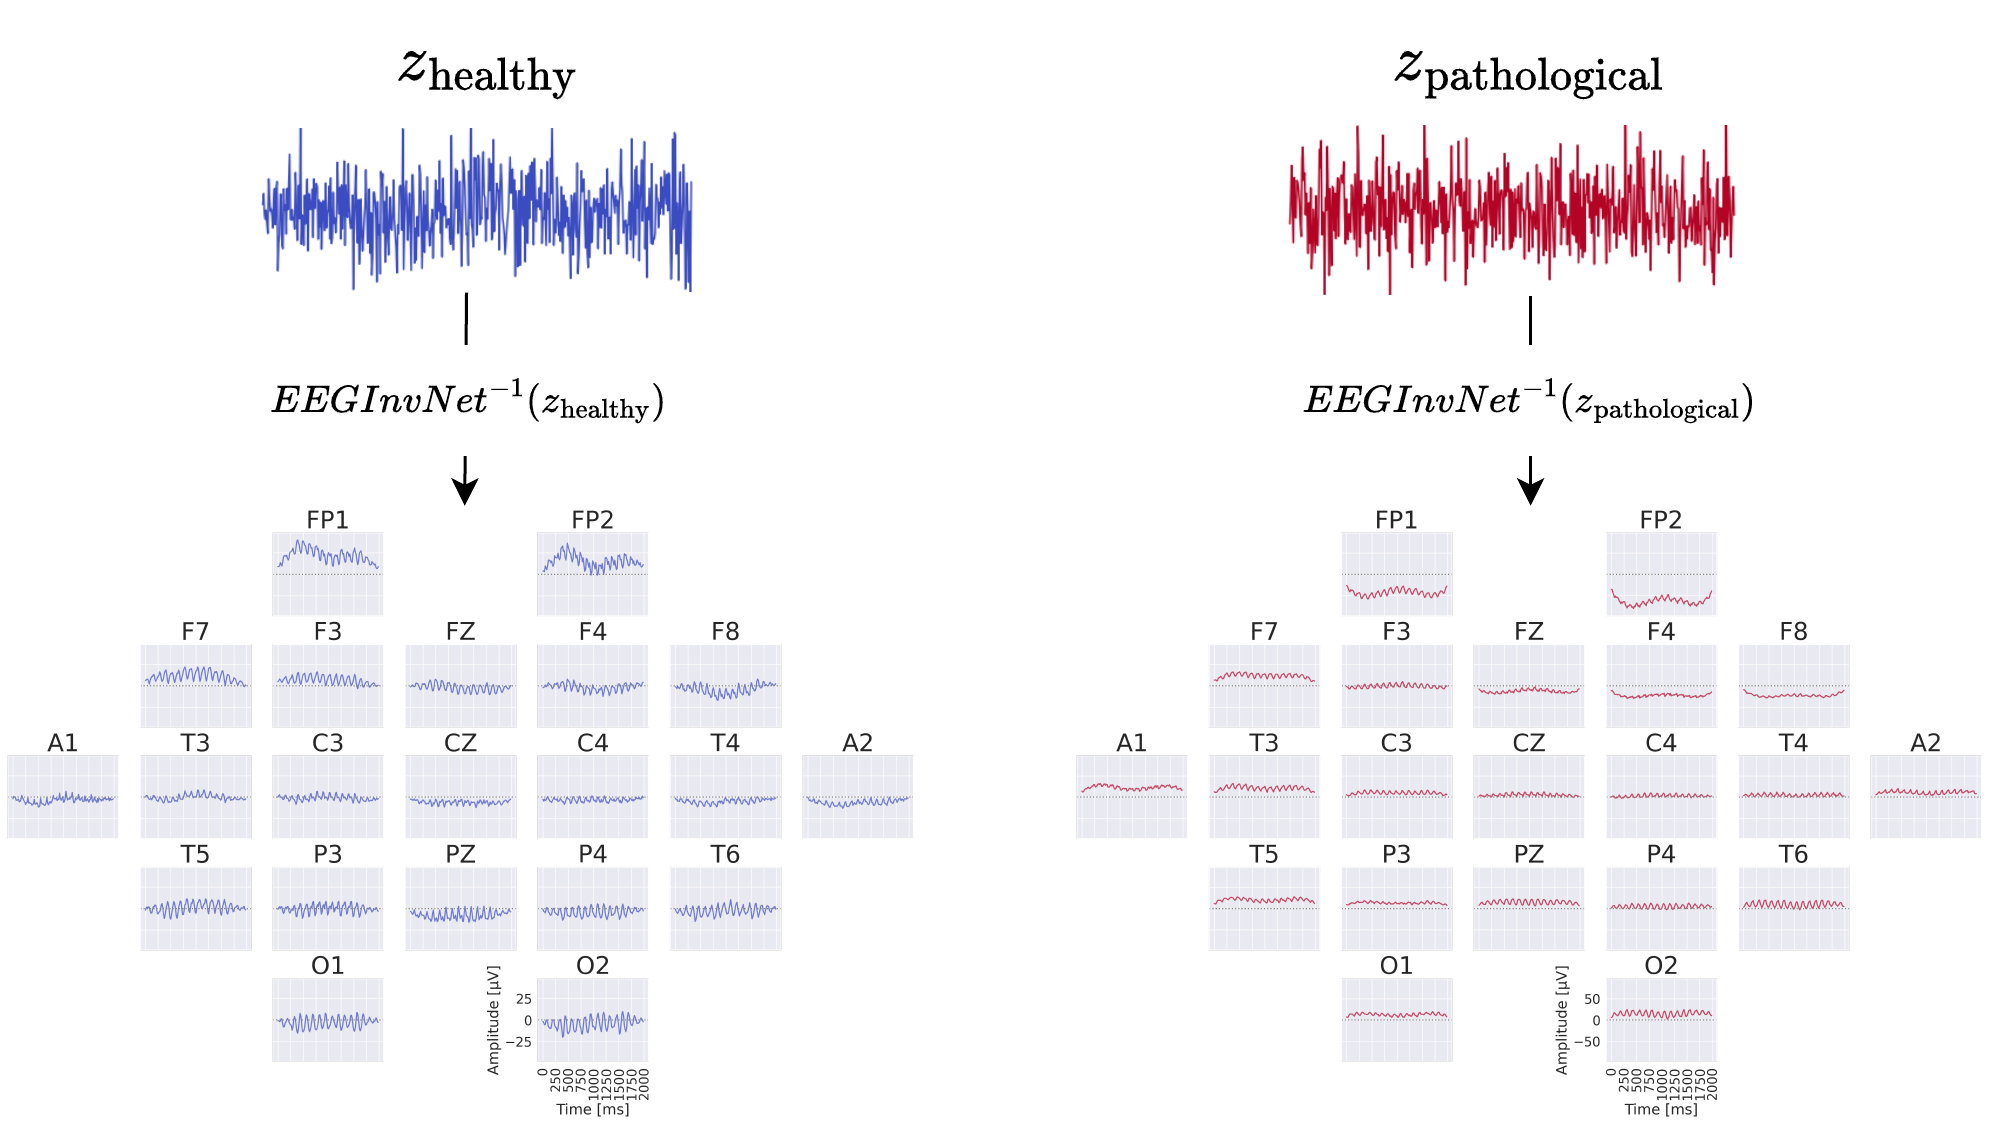
\includegraphics[width=1\linewidth]{images/EEGInvNetClassPrototypes.test.png}
    \caption[EEG-InvNet class prototypes]{
\textbf{EEG-InvNet class prototypes.} Class prototypes are synthesized
by inverting the means $z_\mathrm{healthy}$ and
$z_\mathrm{pathological}$ of the per-class gaussian distributions.
}
\label{eeg-prototypes-fig}
\end{figure}

    In our first visualization, we show the inputs resulting from inverting
the means of the gaussian distributions for each class (see
\Cref{eeg-prototypes-fig}). These can be seen as
prototypical examples of each class and may give hint about the
discriminative features that have been learned. As these are only single
examples, they need to be interpreted cautiously. For example,
individual features within the examples may have a variety of
relationships with the actual prediction function. Consider if a
prototype contains a large alpha-band oscillation at two electrodes,
then these may be indepedendently predictive predictive of that class or
only in combination or even only in some combination with other
features. Nevertheless, the prototypes can already suggest potential
discriminative features for further investigation.

\section{Per-Electrode Prototypes}\label{per-electrode-prototypes}
    

\begin{figure}[h!tb]
    \captionsetup[subfigure]{labelformat=empty}
    \myfloatalign
    \subfloat[]
    {\label{mchan-1}
    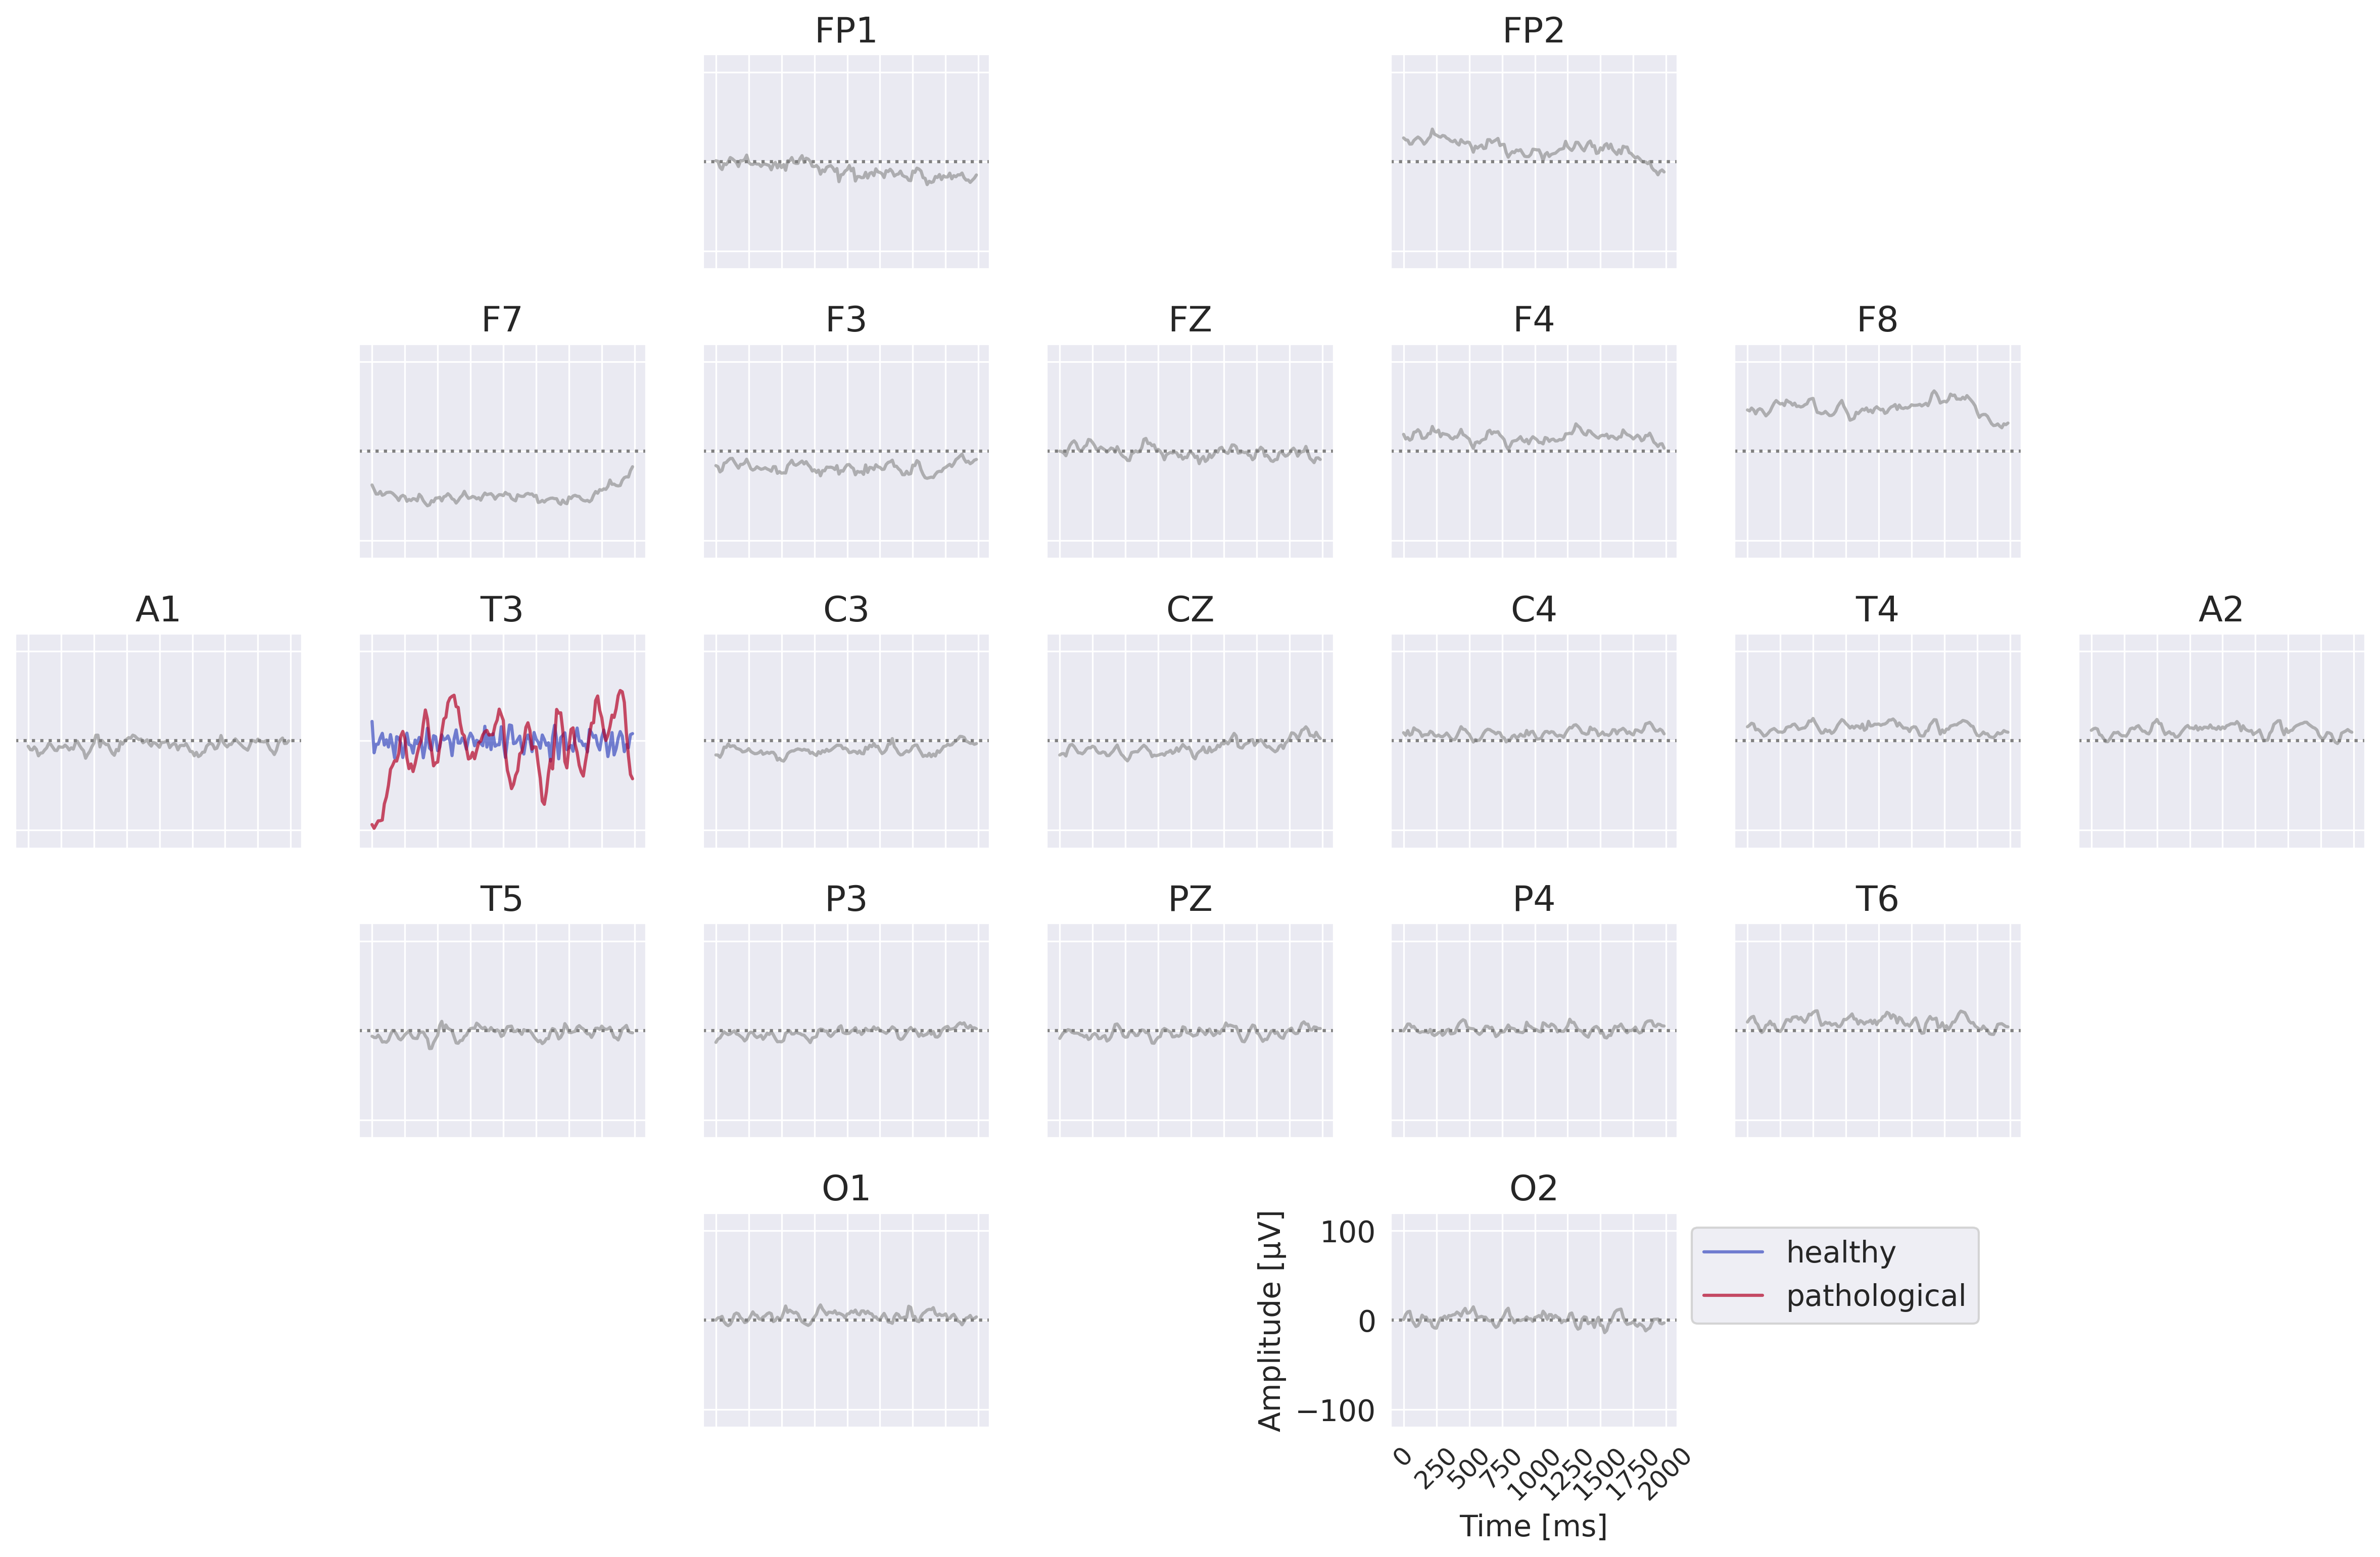
\includegraphics[width=.45\linewidth]{images/marginal-chan-explanation_0.png}} \quad
    \subfloat[] 
    {\label{mchan-2}%
        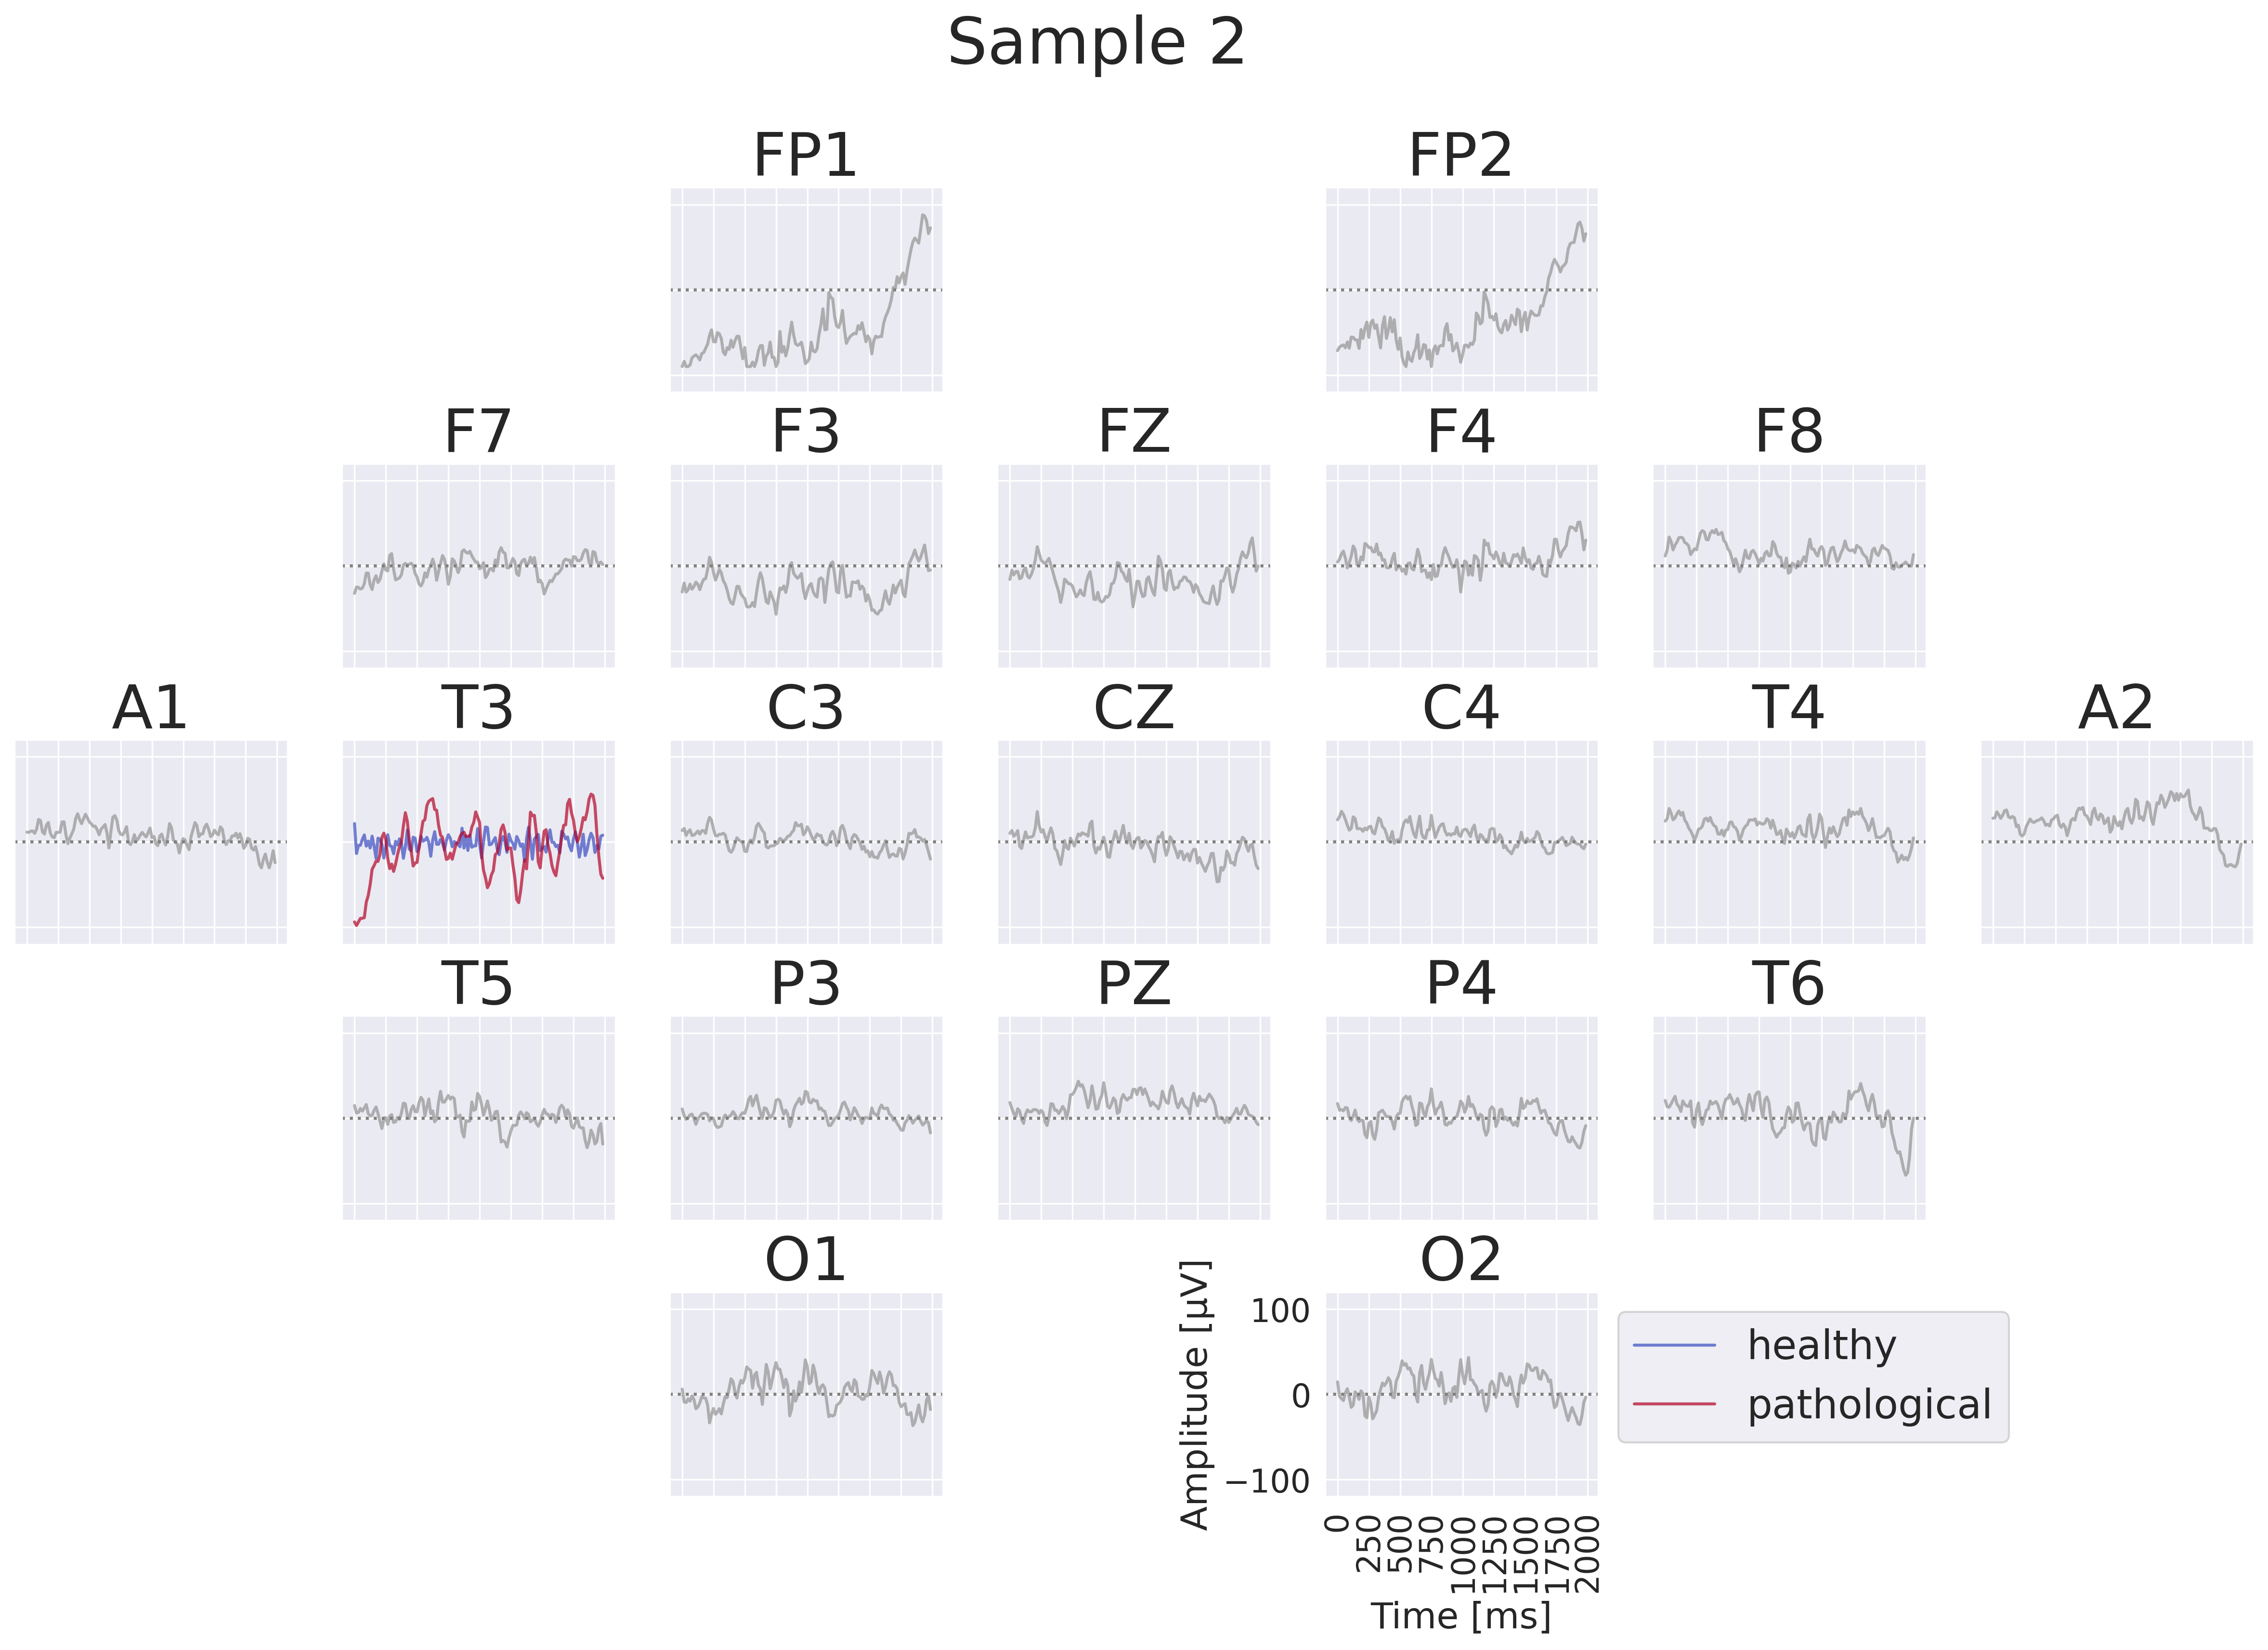
\includegraphics[width=.45\linewidth]{images/marginal-chan-explanation_1.png}} \\
    \subfloat[]
    {\label{mchan-1}
    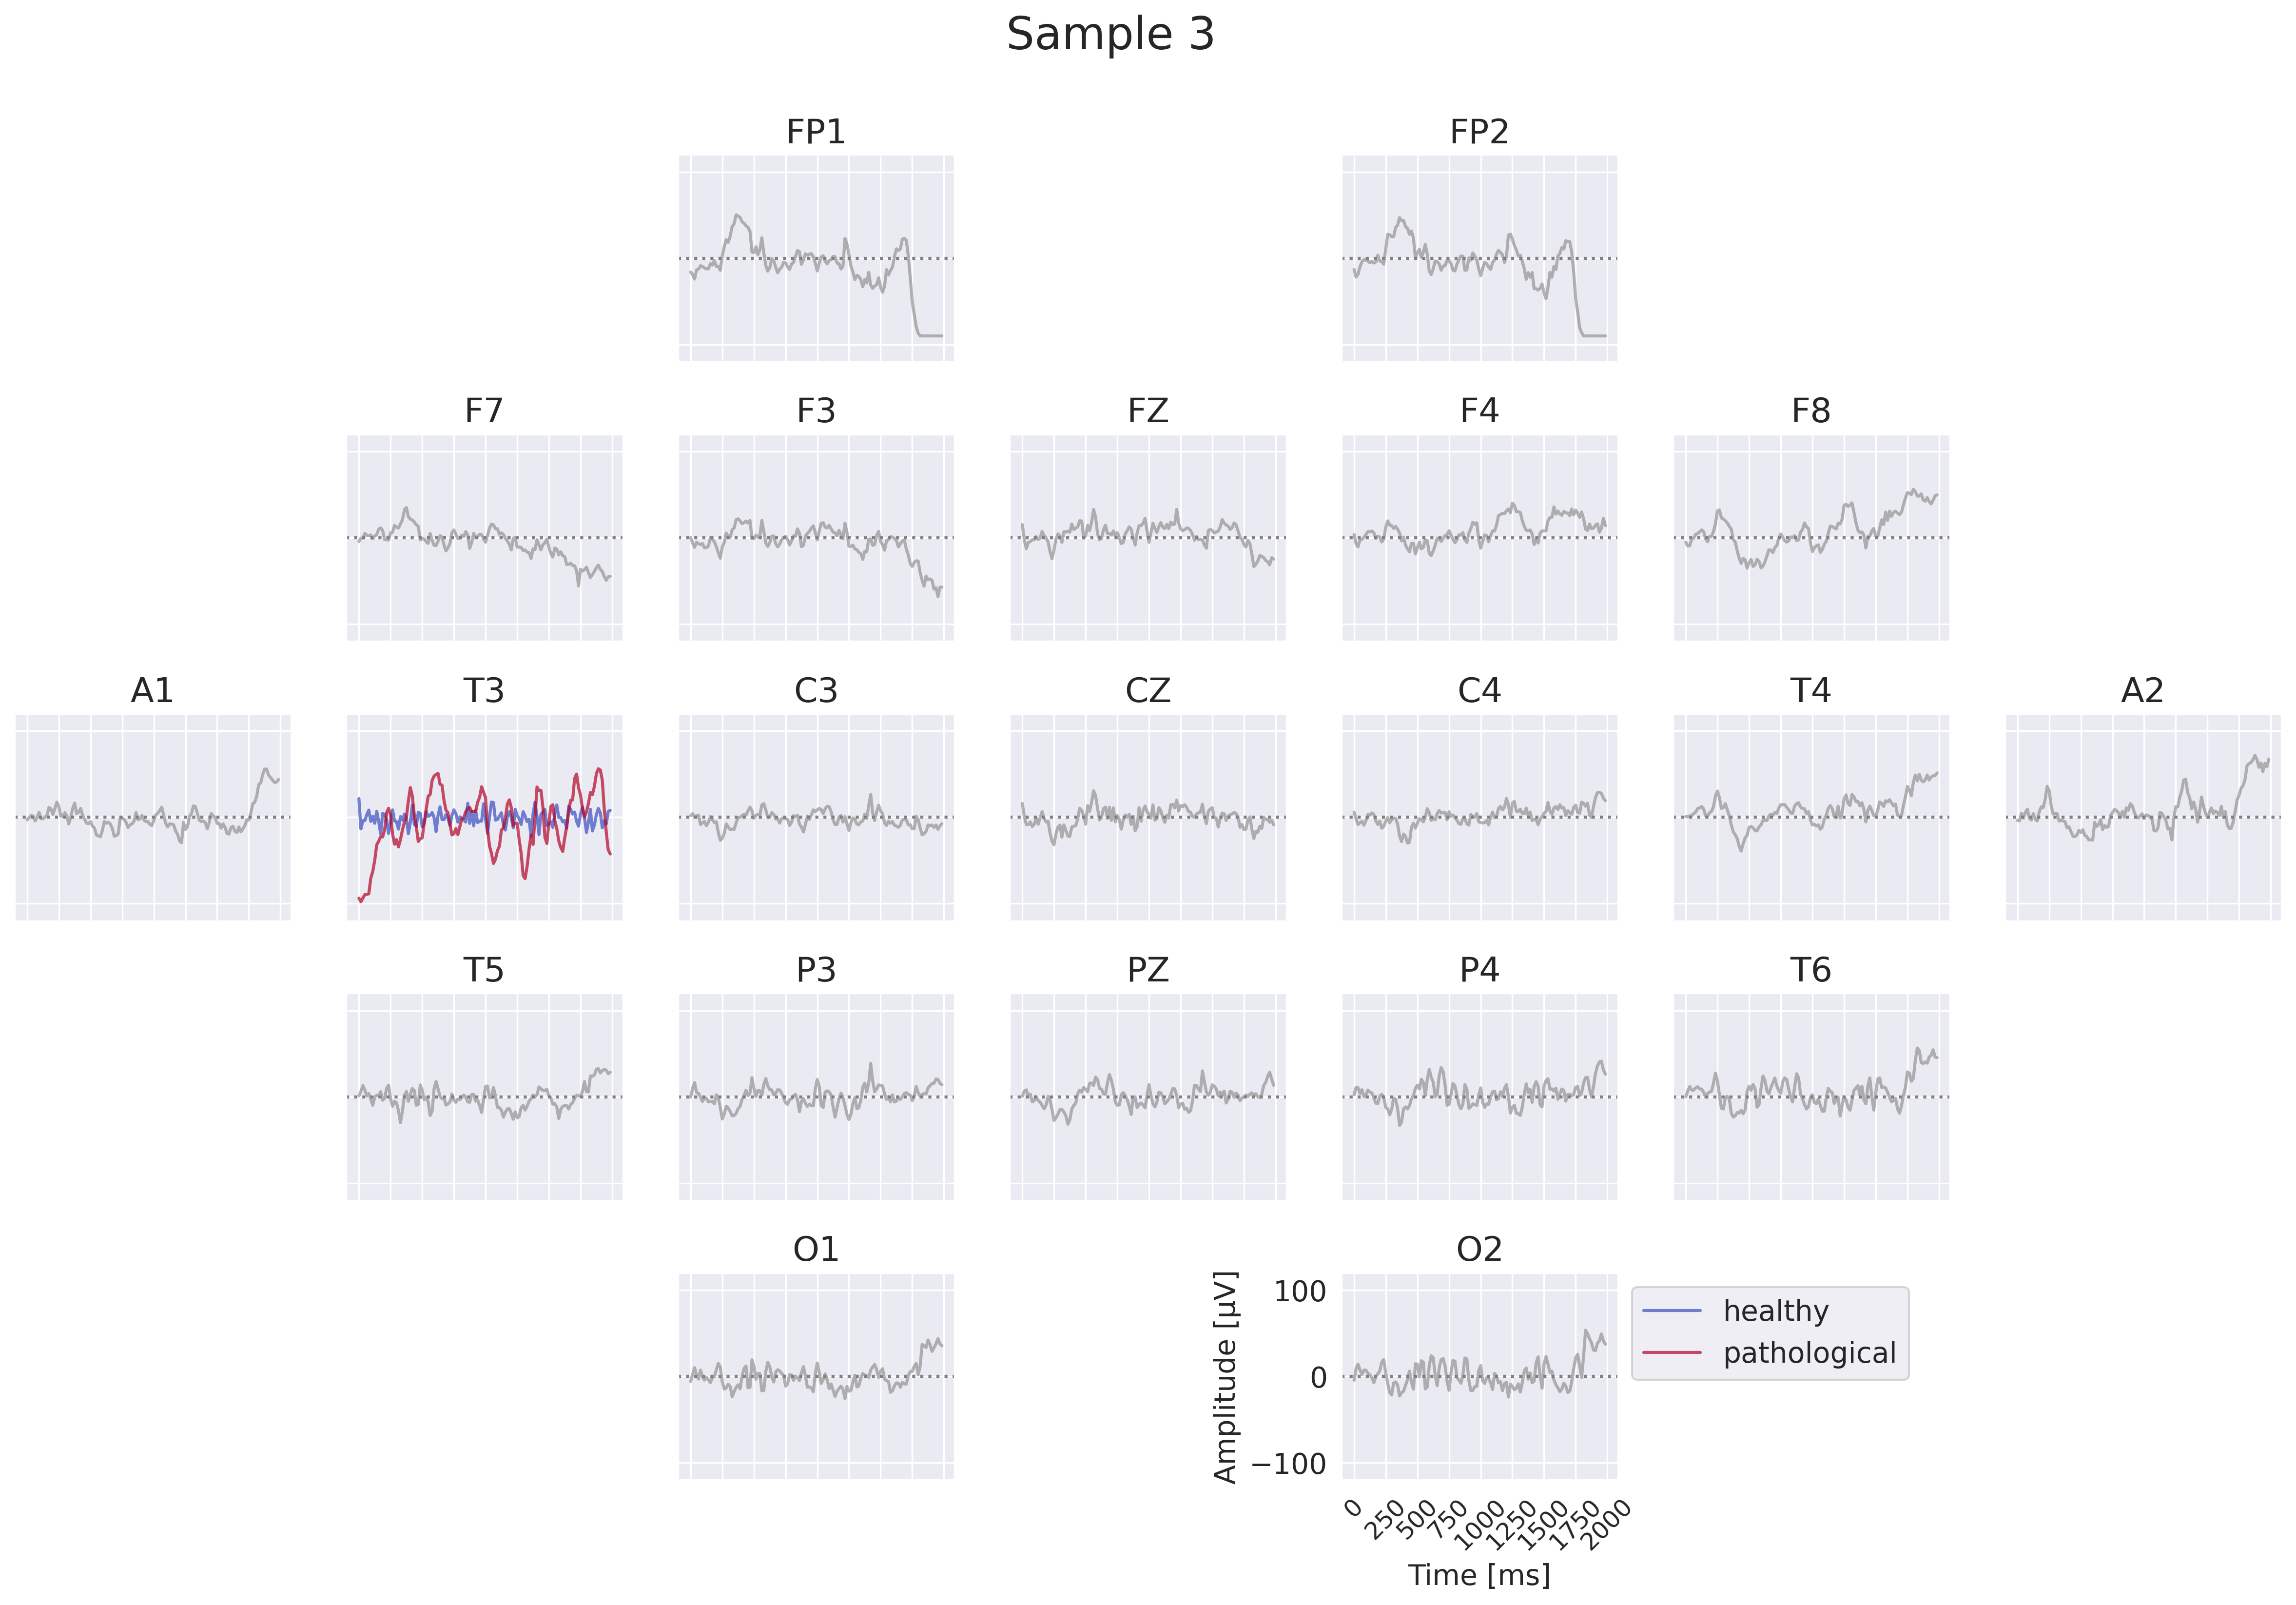
\includegraphics[width=.45\linewidth]{images/marginal-chan-explanation_2.png}} \quad
    \subfloat[]
    {\label{mchan-2}%
        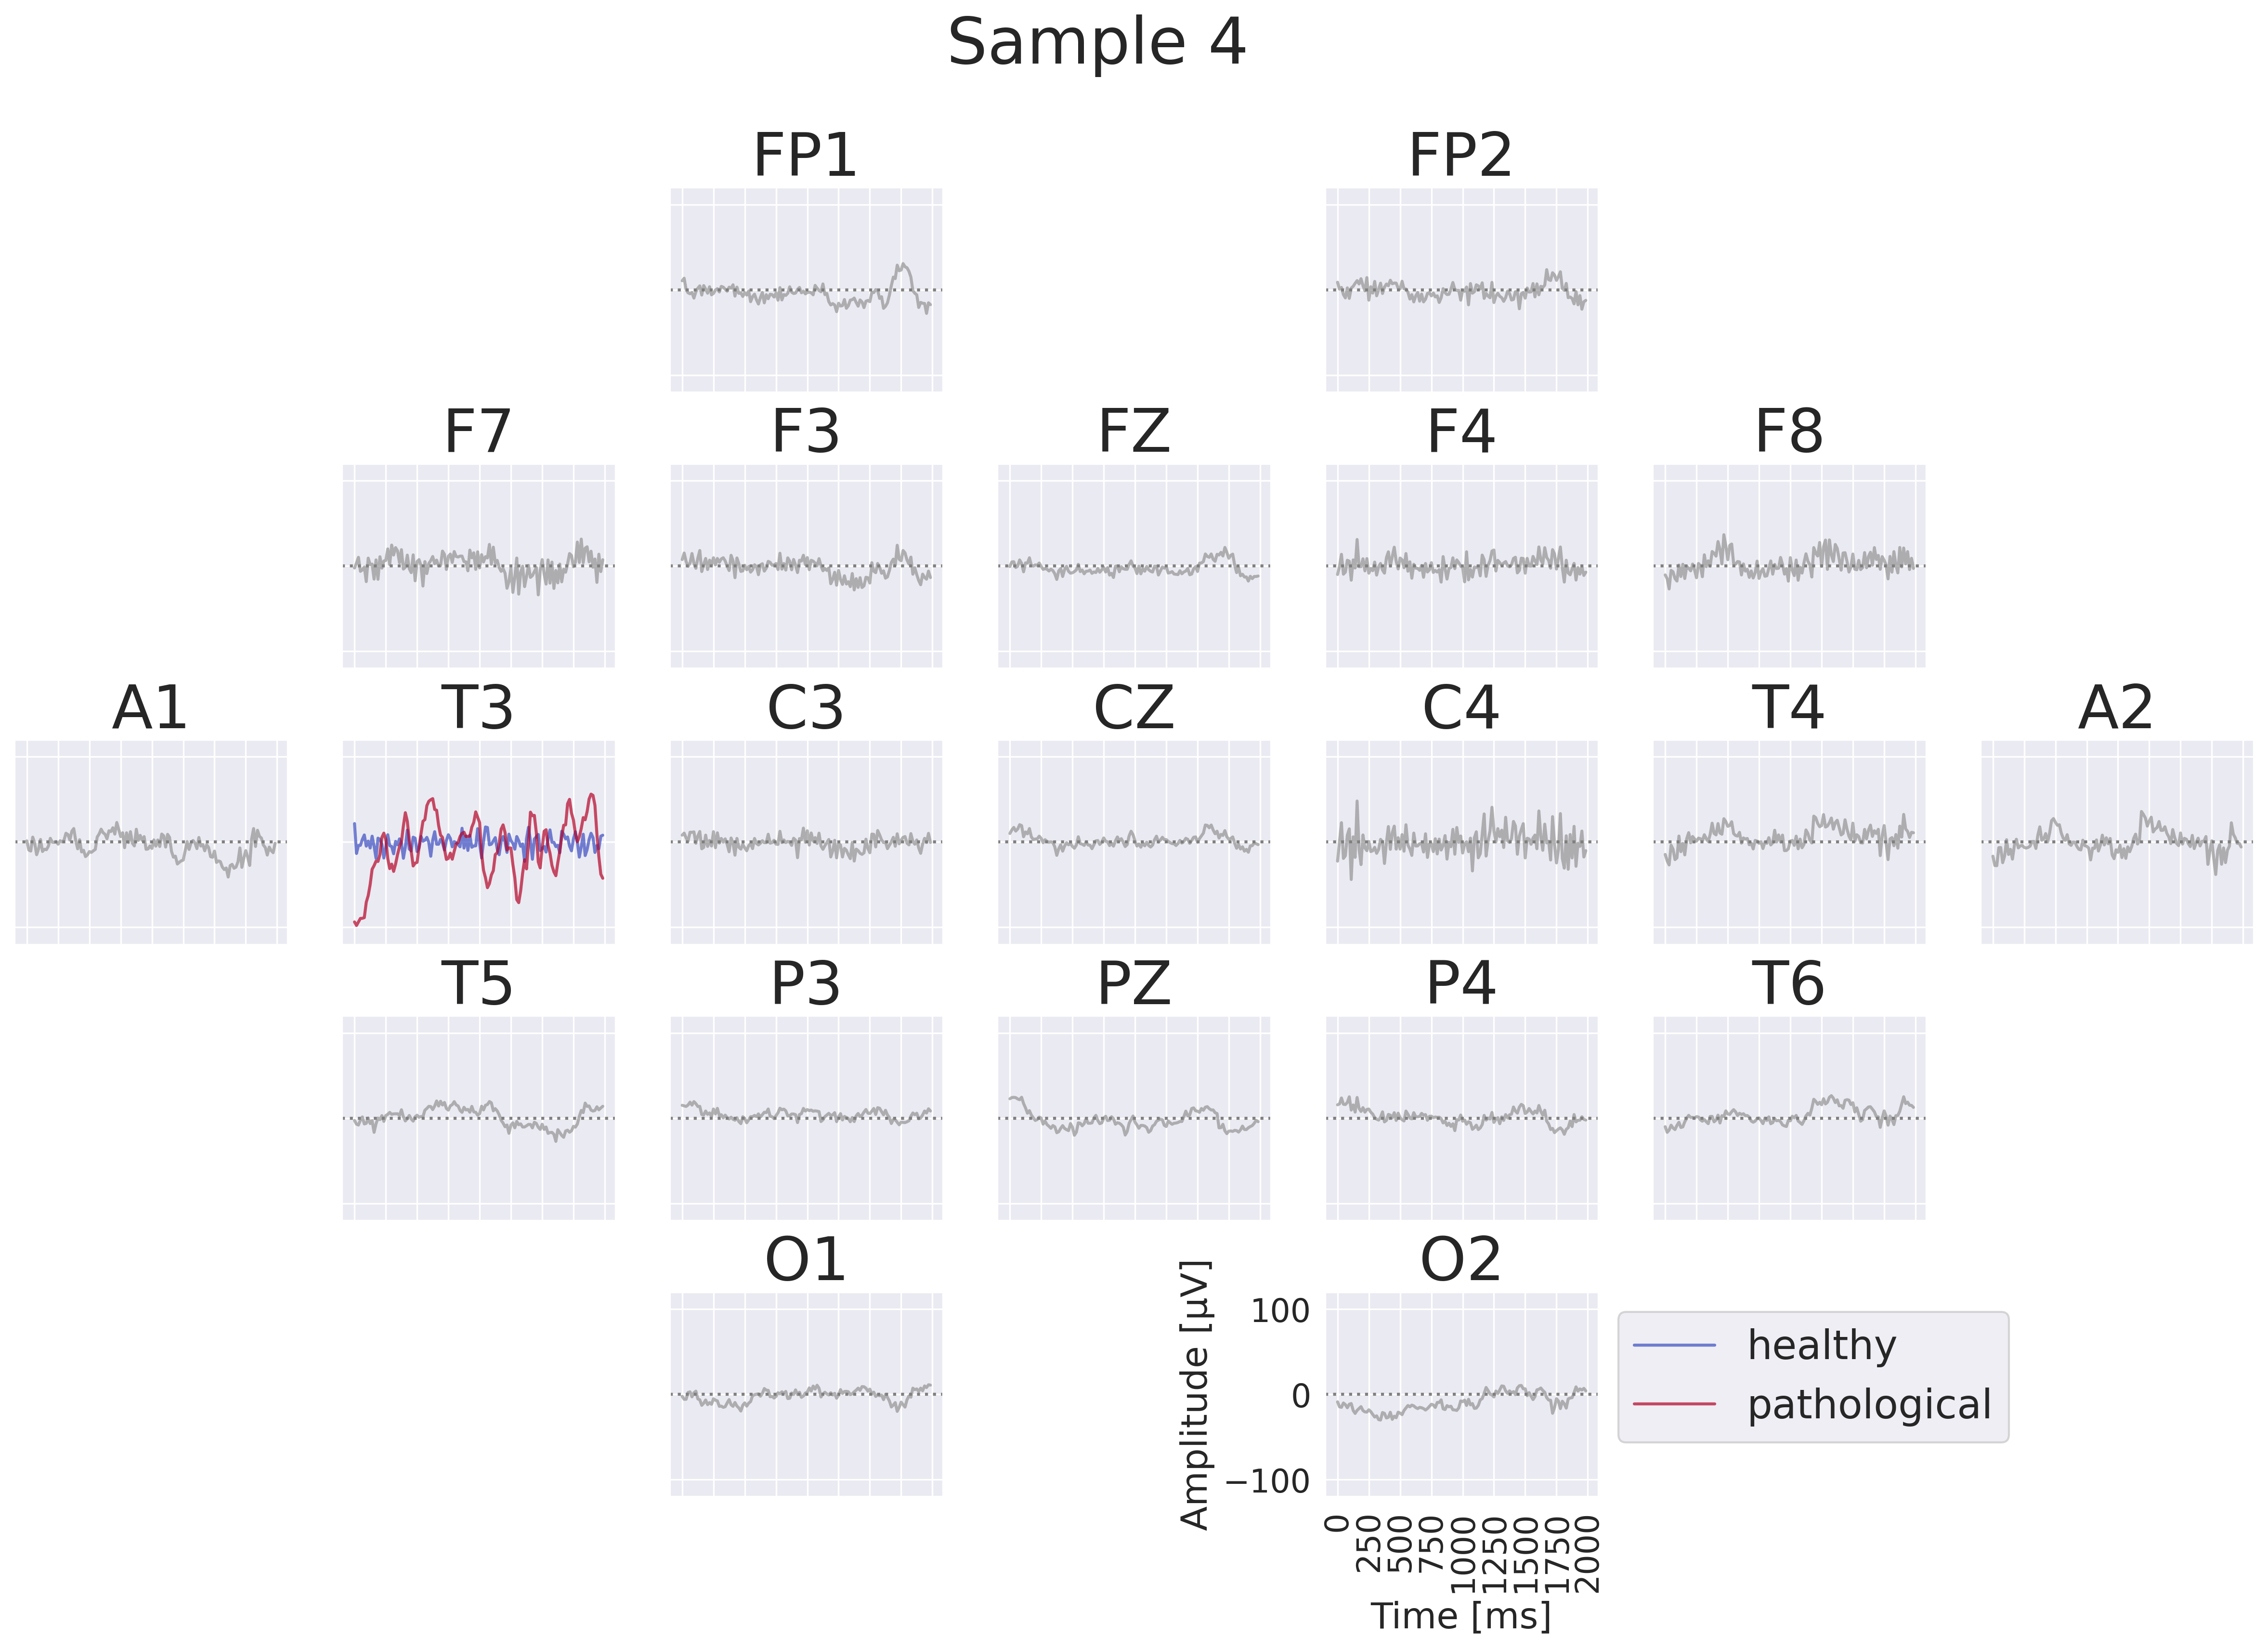
\includegraphics[width=.45\linewidth]{images/marginal-chan-explanation_3.png}} \\
    \caption[EEG-InvNet per-electrode class prototypes]{
    \textbf{EEG-InvNet per-electrode class prototypes.} For getting
per-electrode prototypes, synthetic class-specific signals for one electrode are optimized to yield high predicted class probabilities for any signals at other electrodes.  Signals at other electrodes are sampled from training
data. In the example, prototypes for T3 for the healthy and pathological
class are learned, four samples for remaining electrodes are shown. In
practice, a much larger number of samples would be used. Class signal
probabilities are marginalized over the non-optimized channels as
explained in text.
    }\label{invnet-marginal-chan-explanation-fig}
\end{figure}


    One way to get more interpretable prototypes is to synthesize them per
electrode. Here, we synthesize a signal $x^*_{e_k}$ for a specific
electrode $e_k$ such that the class prediction is high for one class,
independent of the signals at the other electrodes (see
\Cref{invnet-marginal-chan-explanation-fig}). So for
electrode $e_k$ and class $c_i$, we aim to optimize the signal
$x^*_{e_k}$ by maximizing the marginals
$p(x^*_{e_k}|c_i)=\int p(x|c_i;x_{e_k}=x^*_{e_k}) dx$ (generative
loss) and
$p(c_i|x^*_{e_k})=\frac{p(x^*_{e_k}|c_i)}{\sum_j p(x^*_{e_k}|c_j)}$
(classification loss). To approximate this, we sample $n$ signals
$x_l$ of the training distribution and replace the signal
$x_{l,e_k}$ of the electrode $e_k$ we are synthesizing by the
optimized $x^*_{e_k}$. This leads to
$p(x^*_{e_k}|c_i)\approx\sum_{l=1}^n p(x_l|c_i;x_{l,e_k}=x^*_{e_k})$.
While being only a coarse approximation, this already yields insightful
visualizations. For the classification loss, when computing
$p(c_i|x^*_{e_k})$, we found it helpful to first divide the log
probabilities $\log p(x_l|c_i;x_{l,e_k}=x^*_{e_k})$ by the learned
temperature $t$ of the classifier:
$\log p_\mathrm{clf}(x^*_{e_k}|c_i)=\mathrm{logsumexp}\left(\frac{\log p(x_l|c_i;x_{l,e_k}=x^*_{e_k})}{t}\right)$.
Otherwise, $\sum_n p(x_n|c_i;x_{n,e_k}=x^*_{e_k})$ may be dominated by
just a few samples when computing $p(c_i|x^*_{e_k})$. We only apply
this for the classification loss $p(c_i|x^*_{e_k})$, not the
generative loss $p(x^*_{e_k}|c_i)$.

\section{EEG-CosNet}\label{methods-eeg-cosnet}
    

\begin{figure}[htb]
    \captionsetup[subfigure]{labelformat=empty}
    \myfloatalign
    \subfloat[]
    {
    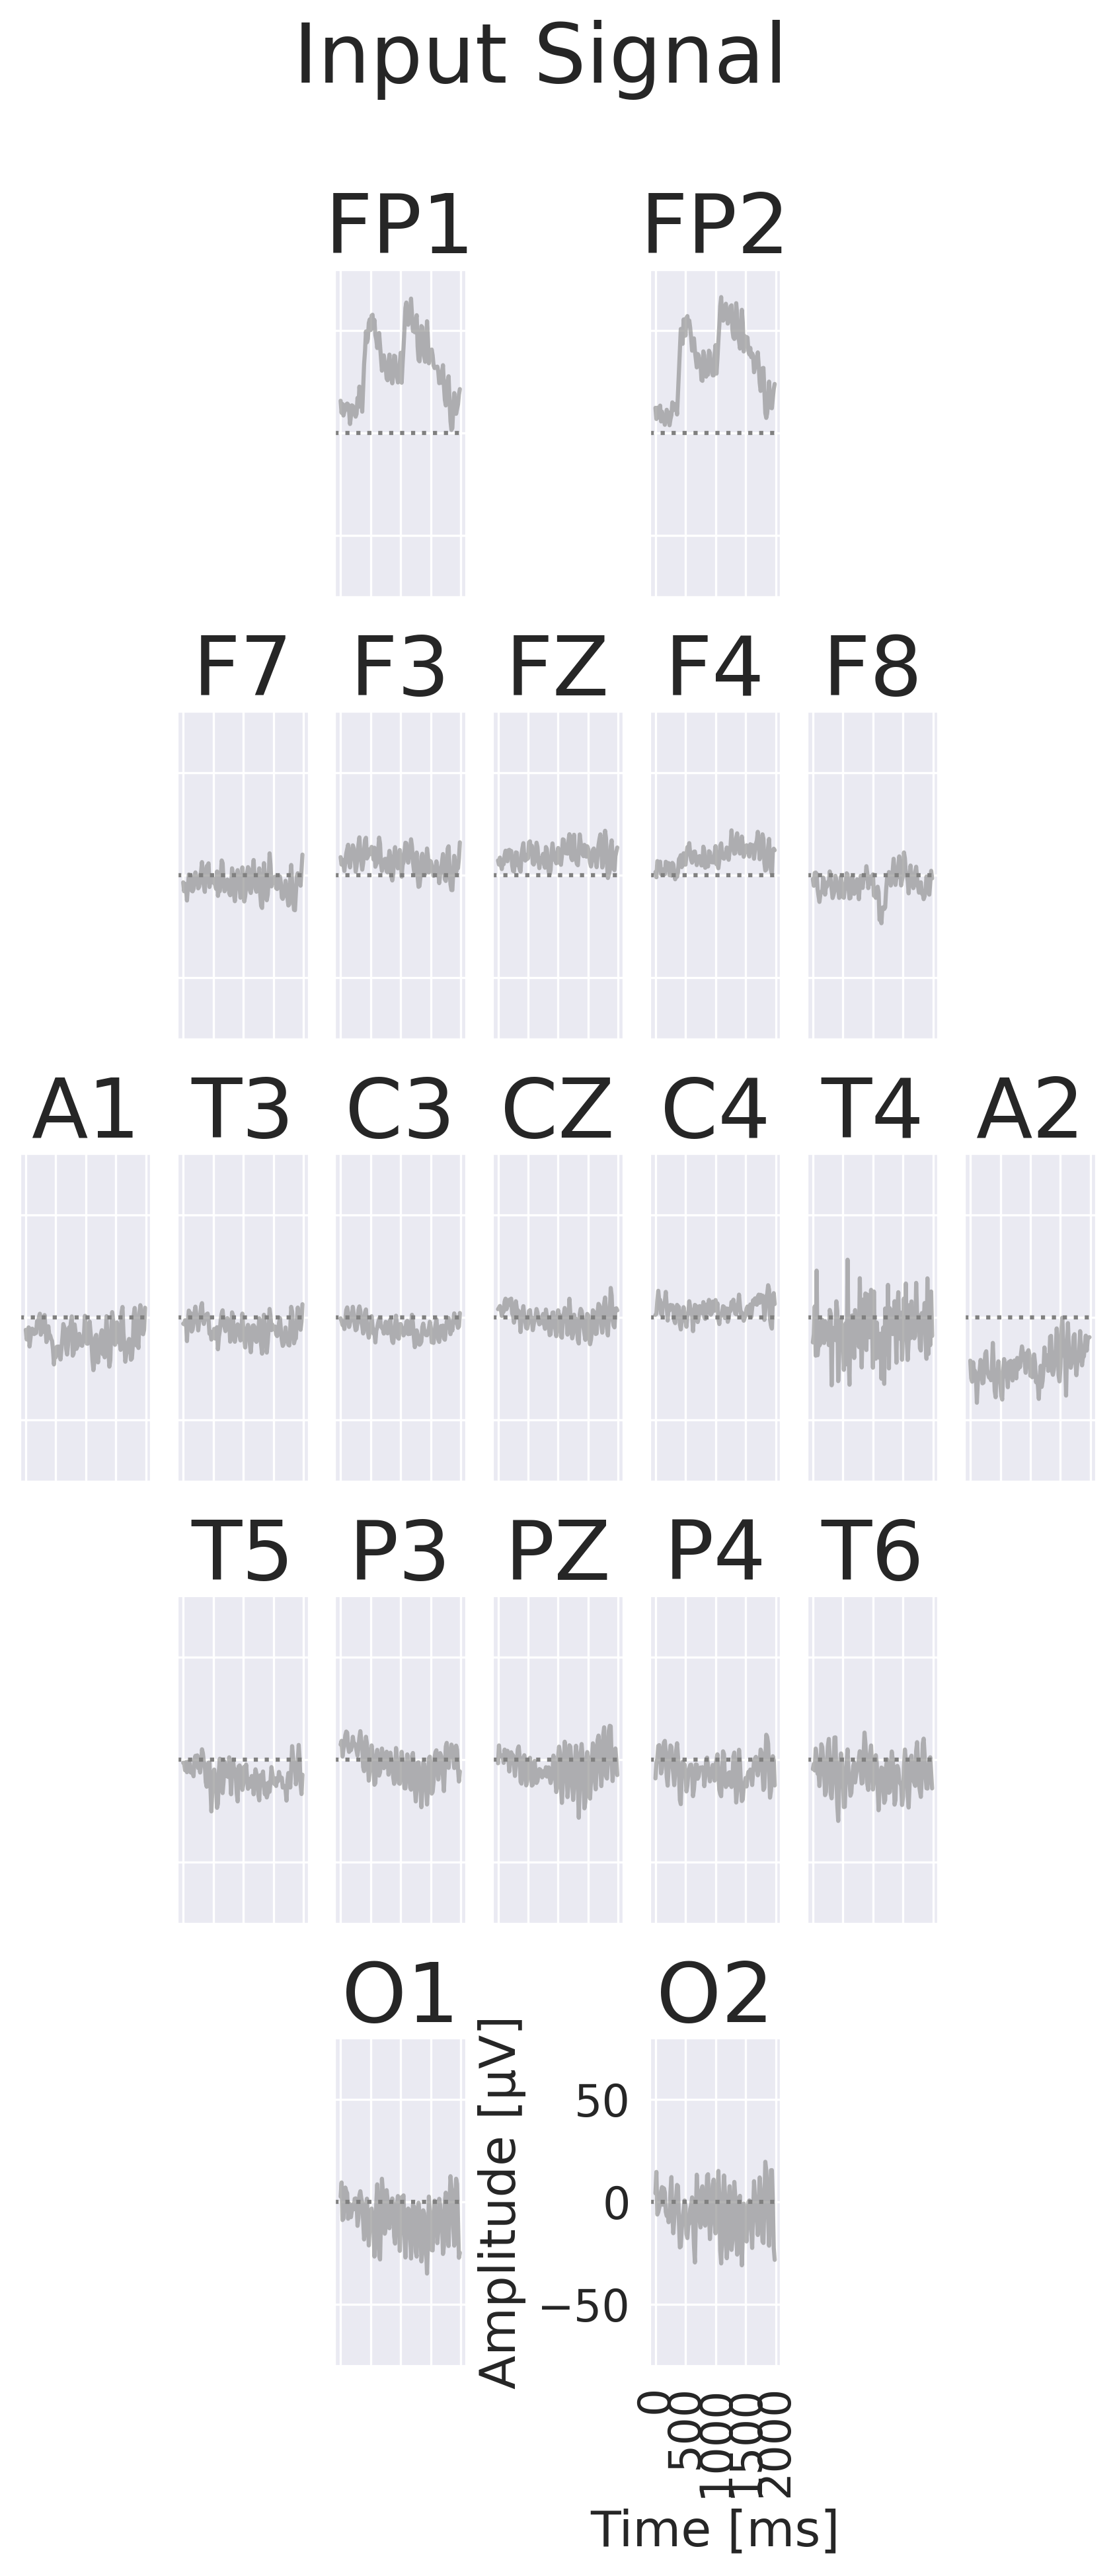
\includegraphics[width=.235\linewidth]{images/cos-net-example-input.png}} \quad
    \subfloat[]
    {
        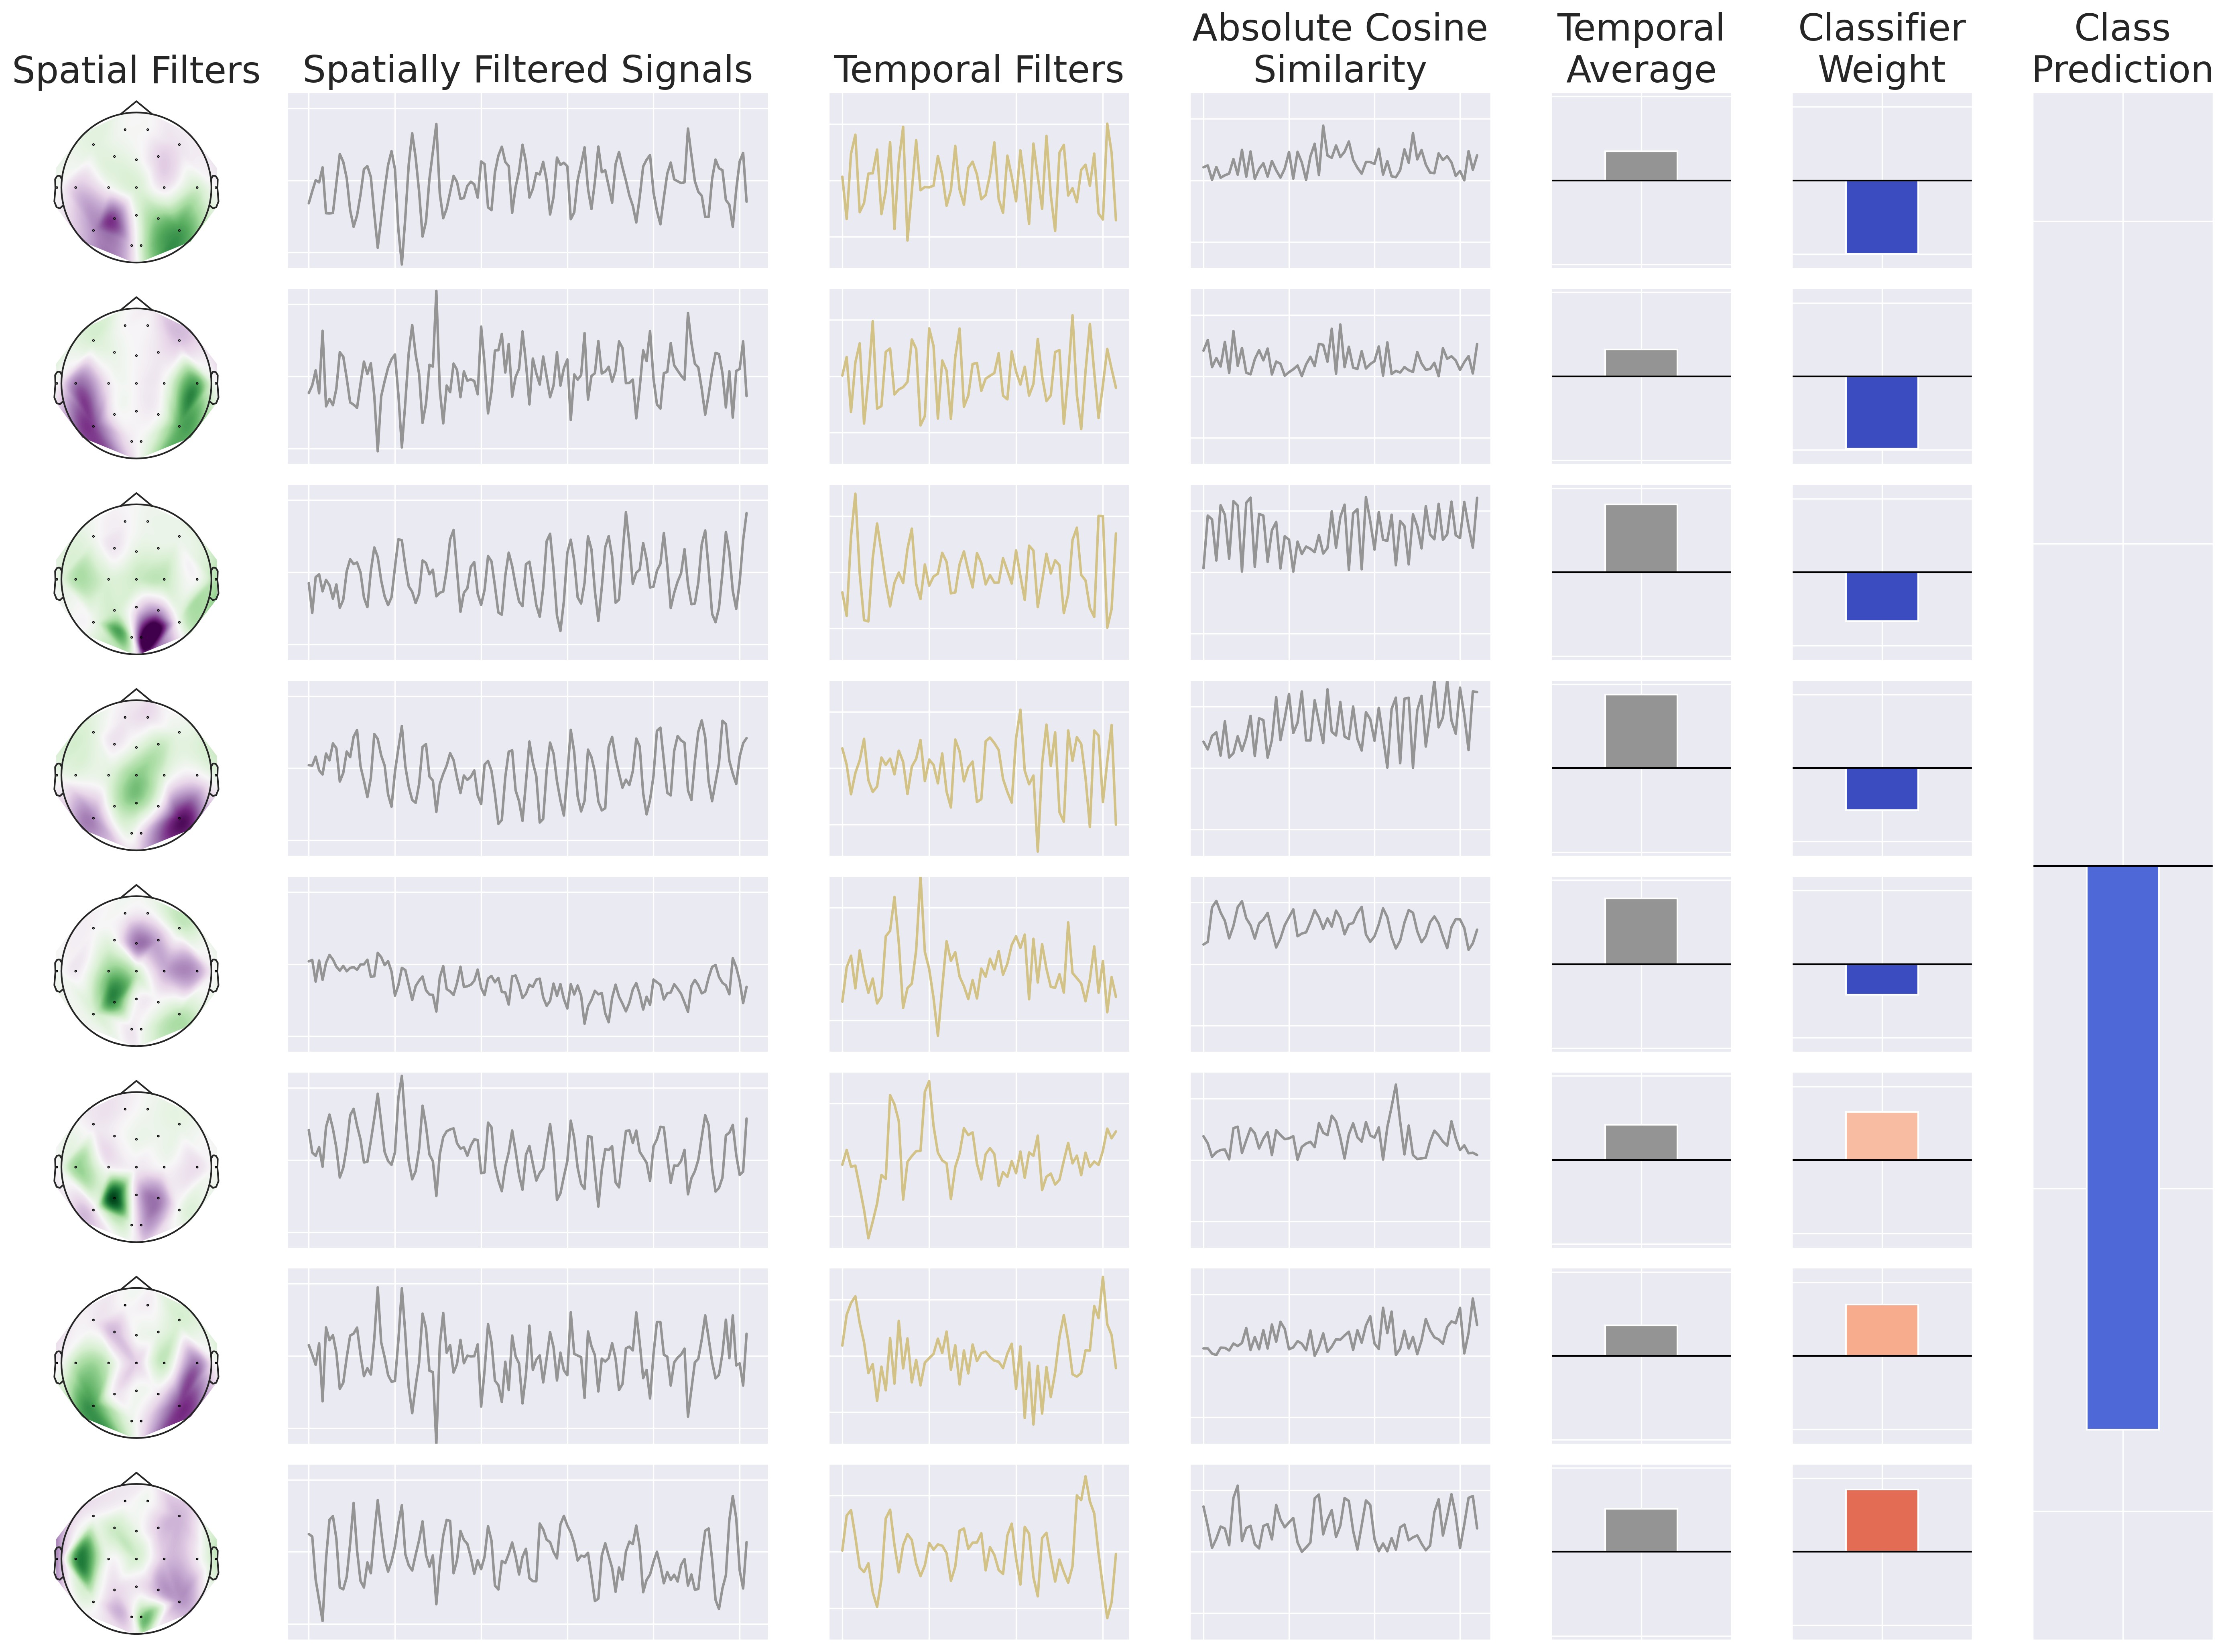
\includegraphics[width=.72\linewidth]{images/cos-net-example-processing.png}} 
    \caption[Example processing of the EEG-CosNet.]{
    \textbf{Example processing of the EEG-CosNet.} Example EEG input on the
left, then processing steps on the right: spatial filtering, absolute
cosine similarity with temporal filters, temporal averaging, then
weighting with linear classifier weights for class prediction. Note the
EEG-CosNet in this visualization only uses 8 filters, whereas later we
will use 64 filters.
}\label{cos-net-example-fig}
\end{figure}


    Finally, we also implemented a small convolutional network EEG-CosNet
that we designed to be directly interpretable. We tried to distill the
trained EEG-InvNet into the EEG-CosNet by training the EEG-CosNet using
the EEG-InvNet class probabilities as the targets for the classification
loss $L_\textrm{class}$. Our EEG-CosNet consists of just three steps
(see \Cref{cos-net-example-fig} for an example computation):


\begin{align*}
    \intertext{\textbf{Spatial Filtering}}
    h_1 &= W_s^Tx && \codecomment{\text{Apply spatial filter weights } W_s \text{ to  inputs }} \\
    \intertext{\textbf{Feature construction}}
    h_2 &= |\mathrm{cos\_sim}(h_1, \mathrm{filters})| && \codecomment{\text{Abs. moving cosine similarity with temporal filters}} \\
    h_3 &=\frac{\sum_t (h_2)}{n_\mathrm{times}} && \codecomment{\text{Average over timepoints in trial}} \\
    \intertext{\textbf{Classification}}
    h_4 &= W_c^Th_3 && \codecomment{\text{Apply classifierweights } W_c \text{ on these features }} \\
p(\mathrm{c_\mathrm{path}}|h_4) &= \frac{1}{1 + \sum_j e^-h_{4}} && \codecomment{\text{Compute sigmoid to get pathological probability}} \\
\end{align*}

Steps 1 and 2 yield spatiotemporal patterns that can be visualized as
waveforms and scalp plots, and that are weighted by the linear
classifier for the respective classes. We chose cosine similarity to
ensure that high output values correspond to spatially filtered signals
that resemble the corresponding temporal filter. The spatial filter
weights and linear classifier weights can be made even more
interpretable through transforming the discriminative weights into
generative patterns by multiplying them with the covariance of the
electrodes/averaged absolute cosine similarities after training, see
\citet{haufe_interpretation_2014} for a discussion on this
technique. We use 64 spatiotemporal filters with temporal length 64
corresponding to one second at 64 Hz.


\begin{openbox}
\item How well can the EEG-InvNet perform on EEG Pathology decoding?
\item What features can the EEG-InvNet reveal?
\item How well can the EEG-CosNet approximate the EEG-InvNet?
\item What features can the EEG-CosNet reveal?
\end{openbox}

%************************************************
\chapter{Decoding Movement-Related Brain Activity}\label{movement-related}
%**************************************
\begin{startbox}{ConvNets can perform as well as FBCSP on movement-related decoding}
\item Shallow network performs best on highpassed data
\item Deep network strongly benefits from cropped training on non-highpassed data
\item Residual network performs well with right initialization
\item Methodological improvements from computer vision improve EEG deep learning decoding
\item Visualizations reveal use of spectral power features with neurophysiologically plausible patterns
\end{startbox}

    Movement-related decoding problems are among the most researched in EEG
decoding and were hence our problem of choice for the first evaluation
of deep learning on EEG. A typical movement-related experimental setting
is that subjects receive a cue for a specific body part (e.g.~right
hand, feet, tongue, etc.) and either move (motor execution) or imagine
to move (motor imagery) this body part. The EEG signals recorded during
the imagined or executed movements then often contain patterns specific
to the body part being moved or thought about. These patterns can then
be decoded using machine learning. In the following, I will describe our
study on movement-related EEG decoding using deep learning, mostly using
content adapted from \citet{schirrmeisterdeephbm2017} and
from \citep{hartmann2018hierarchical}. 

The main study as published in \citet{schirrmeisterdeephbm2017} was carried out
by me as the main author with help of al the coauthors. For
\citet{hartmann2018hierarchical}, Kay Hartmann was the main
contributor and I supported and advised him.

\section{Datasets}\label{datasets}

\subsection{High-Gamma Dataset}\label{high-gamma-dataset}

    Our High-Gamma Dataset is a 128-electrode dataset (of which we later
only use 44 sensors covering the motor cortex) obtained from 14 healthy
subjects (6 female, 2 left-handed, age
27.2$\pm$3.6 (mean$\pm$std)) with roughly 1000 (963.1$\pm$150.9, mean$\pm$std)
four-second trials of executed movements divided into 13 runs per
subject. The four classes of movements were movements of either the left
hand, the right hand, both feet, and rest (no movement, but same type of
visual cue as for the other classes). The training set consists of the
approx. 880 trials of all runs except the last two runs, the test set of
the approx. 160 trials of the last 2 runs. This dataset was acquired in
an EEG lab optimized for non-invasive detection of high-frequency
movement-related EEG components
\citep{ball_movement_2008,darvas_high_2010}. Such
high-frequency components in the range of approx. 60 to above 100 Hz are
typically increased during movement execution and may contain useful
movement-related information
\citep{crone_functional_1998,hammer_predominance_2016,quandt_single_2012}.
Our technical EEG Setup comprised (1.) Active electromagnetic shielding:
optimized for frequencies from DC --- 10 kHz (-30 dB to -50 dB), shielded
window, ventilation \& cable feedthrough (mrShield, CFW EMV-Consulting
AG, Reute, CH) (2.) Suitable amplifiers: high-resolution (24
bits/sample) and low-noise (\textless{}0.6 $\mu V$ RMS 0.16--200 Hz,
1.5 $\mu V$ RMS 0.16--3500 Hz), 5 kHz sampling rate (NeurOne, Mega
Electronics Ltd, Kuopio, FI) (3.) actively shielded EEG caps: 128
channels (WaveGuard Original, ANT, Enschede, NL) and (4.) full optical
decoupling: All devices are battery powered and communicate via optic
fibers.

Subjects sat in a comfortable armchair in the dimly lit Faraday cabin.
The contact impedance from electrodes to skin was typically reduced
below 5 kOhm using electrolyte gel (SUPER-VISC, EASYCAP GmbH,
Herrsching, GER) and blunt cannulas. Visual cues were presented using a
monitor outside the cabin, visible through the shielded window. The
distance between the display and the subjects' eyes was approx. 1 m. A
fixation point was attached at the center of the screen. The subjects
were instructed to relax, fixate the fixation mark and to keep as still
as possible during the motor execution task. Blinking and swallowing was
restricted to the inter-trial intervals. The electromagnetic shielding
combined with the comfortable armchair, dimly lit Faraday cabin and the
relatively long 3-4 second inter-trial intervals (see below) were used
to minimize artifacts produced by the subjects during the trials.

The tasks were as following. Depending on the direction of a gray arrow
that was shown on black background, the subjects had to repetitively
clench their toes (downward arrow), perform sequential finger-tapping of
their left (leftward arrow) or right (rightward arrow) hand, or relax
(upward arrow). The movements were selected to require little proximal
muscular activity while still being complex enough to keep subjects
involved. Within the 4-s trials, the subjects performed the repetitive
movements at their own pace, which had to be maintained as long as the
arrow was showing. Per run, 80 arrows were displayed for 4 s each, with
3 to 4 s of continuous random inter-trial interval. The order of
presentation was pseudo-randomized, with all four arrows being shown
every four trials. Ideally 13 runs were performed to collect 260 trials
of each movement and rest. The stimuli were presented and the data
recorded with BCI2000 \citep{schalk_bci2000:_2004}. The
experiment was approved by the ethical committee of the University of
Freiburg.

\subsection{BCI Competition IV 2a}\label{bci-competition-iv-2a}

    The BCI competition IV dataset 2a is a 22-electrode EEG motor-imagery
dataset, with 9 subjects and 2 sessions, each with 288 four-second
trials of imagined movements per subject (movements of the left hand,
the right hand, the feet and the tongue), for details see
\citet{brunner_bci_2008}. The training set consists of the
288 trials of the first session, the test set of the 288 trials of the
second session.

\subsection{BCI Competition IV 2b}\label{bci-competition-iv-2b}

    The BCI competition IV dataset 2b is a 3-electrode EEG motor-imagery
dataset with 9 subjects and 5 sessions of imagined movements of the left
or the right hand, the latest 3 sessions include online feedback
\citep{leeb_bci_2008}. The training set consists of the
approx. 400 trials of the first 3 sessions
(408.9$\pm$13.7, mean$\pm$std), the test set consists of the approx. 320 trials (315.6$\pm$12.6, mean$\pm$std)of the last two sessions.

\section{Preprocessing}

    We only minimally preprocessed the data to allow the networks to extract
as much information as possible while keeping the input distribution in
a value range suitable for stable network training.

Concretely, our preprocessing steps were:

\begin{enumerate}
\item
  \textbf{Remove outlier trials:} Any trial where at least one channel
  had a value outside +- 800 mV was removed to ensure stable training.
\item
  \textbf{Channel selection:} For the high-gamma dataset, we selected
  only the 44 sensors covering the motor cortex for faster and more
  accurate motor decoding.
\item
  \textbf{High/Bandpass (optional) :} Highpass signal to above 4 Hz.
  This should partially remove potentially informative eye components
  from the signal and ensure that the decoding relies more on brain
  signals. For the BCI competition datasets, in this step we bandpassed
  to 4-38 Hz as using only frequencies until \textasciitilde38-40 Hz was
  commonly done in prior work in this dataset.
\item
  \textbf{Standardization:} Exponential moving standardization as
  described below to make sure the input distribution value range is
  suitable for network training.
\end{enumerate}

Our electrode-wise exponential moving standardization computes
exponential moving means and variances with a decay factor of 0.999 for
each channel and used these to standardize the continuous data.
Formally,

\begin{align}
\mu_t &= 0.001 x_t + 0.999\mu_{t-1}\\
\sigma_t^2 &= 0.001(x_t - \mu_t)^2 + 0.999 \sigma_{t-1}^2\\
x't &= (x_t - \mu_t) / \sqrt{\sigma_t^2}\\
\end{align}

where $x't$ and $x_t$ are the standardized and the original signal
for one electrode at time $t$, respectively. As starting values for
these recursive formulas we set the first 1000 mean values $\mu_t$ and
first 1000 variance values $\sigma_t^2$ to the mean and the variance
of the first 1000 samples, which were always completely inside the
training set (so we never used future test data in our preprocessing).
Some form of standardization is a commonly used procedure for ConvNets;
exponentially moving standardization has the advantage that it is also
applicable for an online BCI.

For FBCSP, this standardization always worsened accuracies in
preliminary experiments, so we did not use it. Overall, the minimal
preprocessing without any manual feature extraction ensured our
end-to-end pipeline could in principle be applied to a large number of
brain-signal decoding tasks as we validated later, see
\Cref{task-related}.

\section{Training Details}\label{training-details}

    As our optimization method, we used Adam
\cite{kingma_adam:_2014} together with a specific early
stopping method, as this consistently yielded good accuracy in
preliminary experiments on the training set. Adam is a variant of
stochastic gradient descent designed to work well with high-dimensional
parameters, which makes it suitable for optimizing the large number of
parameters of a ConvNet \cite{kingma_adam:_2014}. The early
stopping strategy that we use throughout these experiments, developed in
the computer vision field \footnote{https://web.archive.org/web/20160809230156/https://code.google.com/p/cuda-convnet/wiki/Methodology},
splits the training set into a training and validation fold and stops
the first phase of the training when validation accuracy does not
improve for a predefined number of epochs. The training continues on the
combined training and validation fold starting from the parameter values
that led to the best accuracies on the validation fold so far. The
training ends when the loss function on the validation fold drops to the
same value as the loss function on the training fold at the end of the
first training phase (we do not continue training in a third phase as in
the original description). Early stopping in general allows training on
different types of networks and datasets without choosing the number of
training epochs by hand. Our specific strategy uses the entire training
data while only training once. In our study, all reported accuracies
have been determined on an independent test set.

    Note that in later works we do not use this early stopping method
anymore as we found training on the whole training set with a cosine
learning rate schedule \cite{DBLP:conf/iclr/LoshchilovH17} to
lead to better final decoding performance.

\section{Design Choices}\label{design-choices}



\begin{table}[ht]
    \small
    \myfloatalign
    \begin{tabularx}{\textwidth}{p{0.16\textwidth}p{0.16\textwidth}p{0.16\textwidth}p{0.4\textwidth}} \toprule
        \tableheadlinewithwidth{0.16\textwidth}{\large Design aspect} &
        \tableheadlinewithwidth{0.16\textwidth}{\large Our Choice} & \tableheadlinewithwidth{0.16\textwidth}{\large Variants} & \tableheadlinewithwidth{0.4\textwidth}{\large Motivation}\\ 
        \midrule
    Activation functions & ELU & Square, ReLU & We expected these choices to
be sensitive to the type of feature (e.g., signal phase or power), as
squaring and mean pooling results in mean power (given a zero-mean
signal). Different features may play different roles in the
low-frequency components vs the higher frequencies (see the section
``Datasets and Preprocessing''). \\
Pooling mode & Max & Mean & (see above) \\
Regulariza-tion and intermediate normalization & Dropout + batch normalization + a new tied loss function (explanations see text) &Only
 batch normalization, only dropout, neither of both, nor tied loss & We
wanted to investigate whether recent deep learning advances improve
accuracies and check how much regularization is required. \\
Factorized temporal convolutions & One 10 x 1 convolution per
convolutional layer & Two 6 x 1 convolutions per convolutional layer &
Factorized convolutions are used by other successful ConvNets \citep{szegedy_rethinking_2015} \\
Splitted vs one-step convolution & Splitted convolution in first layer (see \Cref{shallow-convnet-architecture}) &  One-step
convolution in first layer & Factorizing convolution into spatial and
temporal parts may improve accuracies for the large number of EEG input
channels (compared with three rgb color channels of regular image
datasets). \\
        \bottomrule
    \end{tabularx}
    \caption[Evaluated design choices]{\textbf{Evaluated design choices.}}  
    \label{design-choices-table}
\end{table}


For the shallow and deep network, we evaluated how a number of design
choices affect the final accuracies, see \Cref{design-choices-table}.

\subsection{Tied Loss Function}\label{tied-loss-function}

Our tied loss function penalizes the discrepancy between neighbouring
predictions. Concretely, in this \emph{tied sample loss function}, we
added the cross-entropy of two neighboring predictions to the usual loss
of of negative log likelihood of the labels. So, denoting the predicted
probabilties $p\big(l_k|f_k(X^j_{t..t+T'};\theta)\big)$ for crop
$X^j_{t..t+T'}$ with label $l_k$ from time step $t$ to $t+T'$ by
$p_{f,k}(X^j_{t..t+T'})$, the loss now also depends on the predicted
probabilties for the next crop $p_{f,k}(X^j_{t..t+T'+1})$ and is then:
% 

\begin{equation}
\begin{split}
 \textrm{loss}\big(y^j, p_{f,k}(X^j_{t..t+T'})\big) &= \sum_{k=1}^{K}-log\big(p_{f,k}(X^j_{t..t+T'})\big)\cdot \delta(y^j=l_k) \\
 &+ \sum_{k=1}^{K}-log\big(p_{f,k}(X^j_{t..t+T'})\big) \cdot p_{f,k}(X^j_{t..t+T'+1})
\end{split}
\end{equation}



This is meant to make the ConvNet focus on features which are stable for
several neighboring input crops.

\section{Results}\label{results}

\subsection{Validation of FBCSP Pipeline}\label{validation-of-fbcsp-pipeline}

    As a first step before moving to the evaluation of ConvNet decoding, we
validated our FBCSP implementation, as this was the baseline we compared
the ConvNets results against. To validate our FBCSP implementation, we
compared its accuracies to those published in the literature for the BCI
competition IV dataset 2a \citep{sakhavi_parallel_2015}.
Using the same 0.5--2.5 s (relative to trial onset) time window, we
reached an accuracy of 67.6\%, statistically not significantly different
from theirs (67.0\%, p=0.73, Wilcoxon signed-rank test). Note however,
that we used the full trial window for later experiments comparing
against convolutional networks, i.e., from 0.5--4 seconds. This yielded
a slightly better accuracy of 67.8\%, which was still not statistically
significantly different from the original results on the 0.5--2.5 s
window (p=0.73). For all later comparisons, we use the 0.5--4 seconds
time window on all datasets.

\subsection{Filterbank Network}\label{filterbank-network}

\begin{table}[ht]
    \myfloatalign
    \begin{tabularx}{\textwidth}{llll}
    \toprule
        \tableheadlinewithwidth{0.2\textwidth}{Decoding method} & \tableheadlinewithwidth{0.2\textwidth}{Sampling rate} &
        \tableheadlinewithwidth{0.2\textwidth}{Test Accuracy [\%]}  & 
        \tableheadlinewithwidth{0.2\textwidth}{Std [\%]} 
        \\
        \midrule
        FBCSP & 300 & 88.1 & 13.9 \\
        FBCSP & 150 & 86.7 & 14.3 \\
        Filterbank Net & 300 & 90.5 & 10.4 \\
        Filterbank Net & 150 & 87.9 & 13.9 \\
        \bottomrule
    \end{tabularx}
    \caption[Filterbank Net vs FBCSP Accuracies.]{\textbf{Filterbank Net vs FBCSP Accuracies.} Std is standard deviation over the 18 subjects used here. Results from \citet{schirrmeister_msc_thesis_2015}.}  \label{filterbank-net-results}
\end{table}


    Prior to our more extensive study, we had evaluated the filterbank
network on a different version of the High-Gamma Dataset in a master
thesis \citep{schirrmeister_msc_thesis_2015}. This version
of the dataset included different subjects, as some subjects had not
been recorded yet and other subjects were later excluded for the work
here due to the presence of too many artifacts. Furthermore, we
evaluated 150Hz and 300 Hz as sampling rates here, in the remainder we
will use 250 Hz.

The results in \Cref{filterbank-net-results} show that the
Filterbank net outperformed FBCSP by 2.4\% (300 Hz) and 1.3\% (150 Hz)
respectively. Despite the good performance, we did not evaluate this
network further after the master thesis due to the very large GPU memory
requirement of our implementation and our interest in evaluating more
expressive architectures not as tightly constrained to implement FBCSP
steps.

\subsection{ConvNets Reached FBCSP
Accuracies}\label{convnets-reached-fbcsp-accuracies}


\begin{figure}[h!tb]
    \myfloatalign
    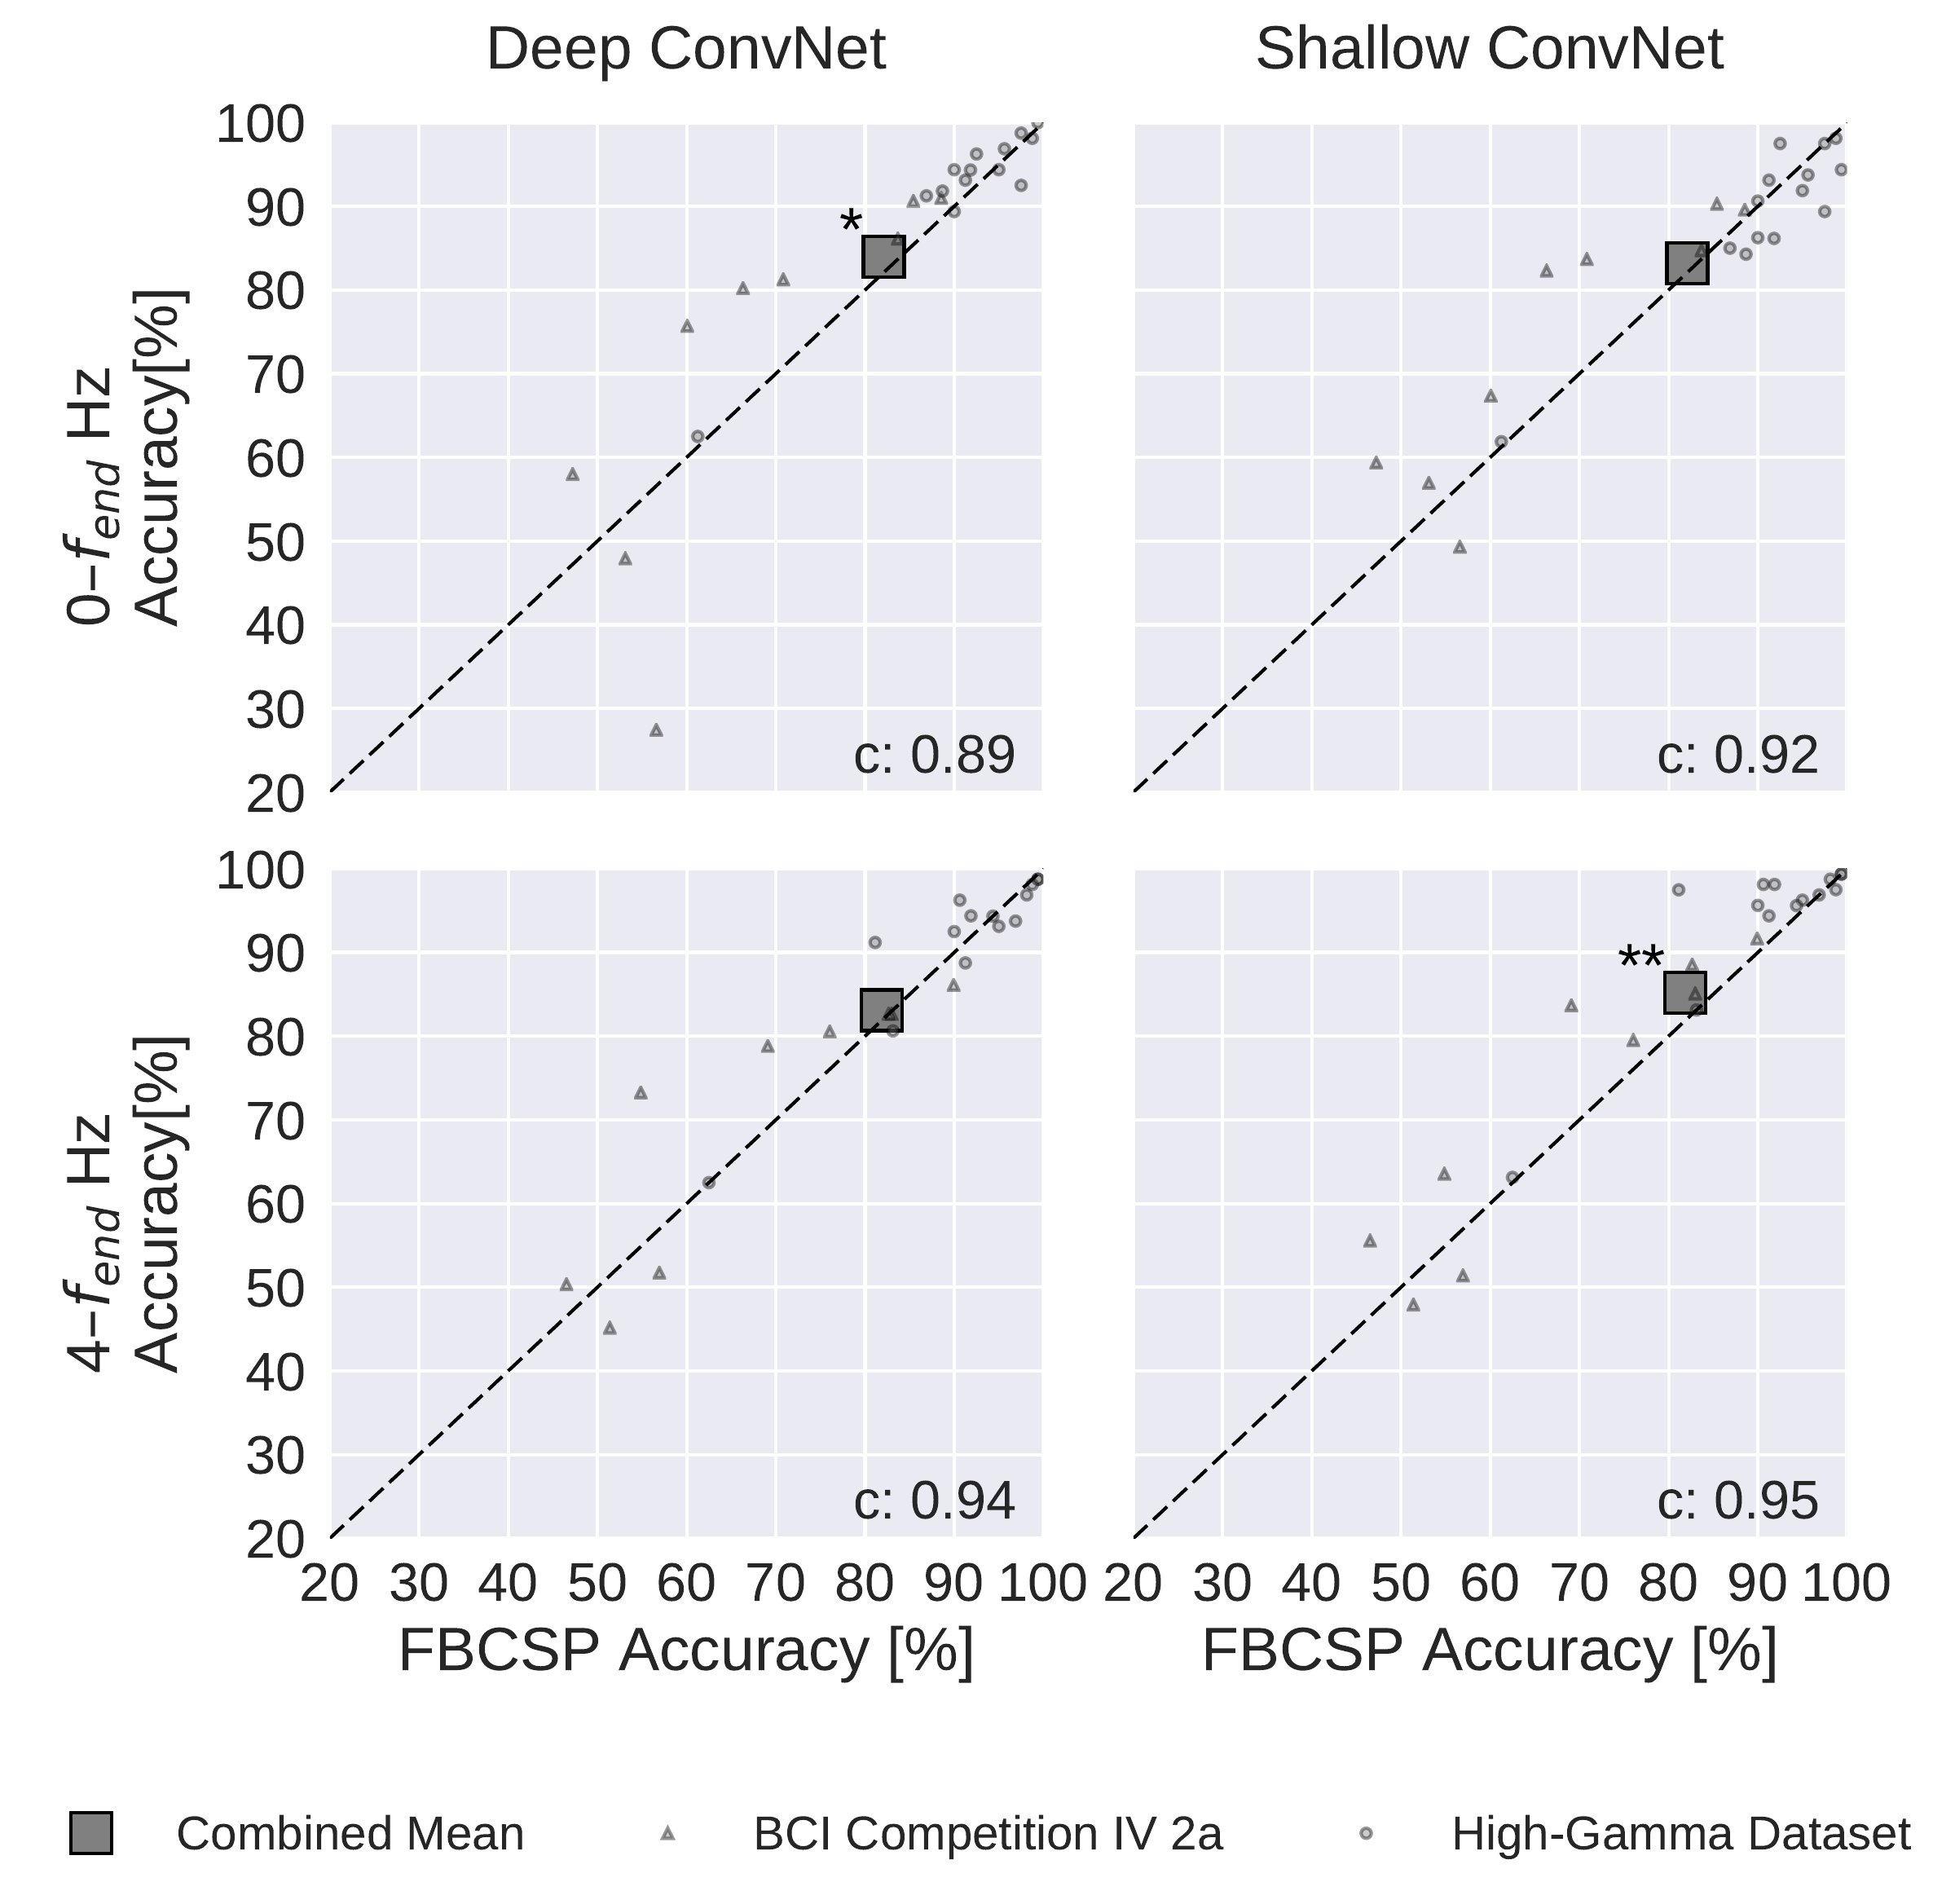
\includegraphics[width=0.9\linewidth]{images/Final_Comparison.ipynb.2.png}
    \caption[FBCSP vs. ConvNet decoding accuracies.]{
\textbf{FBCSP vs. ConvNet decoding accuracies.} Each small marker
represents accuracy of one subject, the large square markers represent
average accuracies across all subjects of both datasets. Markers above
the dashed line indicate experiments where ConvNets performed better
than FBCSP and opposite for markers below the dashed line. Stars
indicate statistically significant differences between FBCSP and
ConvNets (Wilcoxon signed-rank test, p\textless0.05: *, p\textless0.01:
**, p\textless0.001:***). Bottom left of every plot: linear correlation
coefficient between FBCSP and ConvNet decoding accuracies. Mean
accuracies were very similar for ConvNets and FBCSP, the (small)
statistically significant differences were in direction of the ConvNets.
Figure from \citet{schirrmeisterdeephbm2017}.
}
\label{movement-decoding-result-comparison-figure}
\end{figure}


\begin{table}[htb]
    \myfloatalign
    \begin{tabularx}{\textwidth}{lllll}
    \toprule
        \tableheadlinewithwidth{0.25\textwidth}{Dataset} & \tableheadlinewithwidth{0.2\textwidth}{Frequency Range (Hz)} &
        \tableheadlinewithwidth{0.12\textwidth}{FBCSP}  & 
        \tableheadlinewithwidth{0.12\textwidth}{Deep} & 
        \tableheadlinewithwidth{0.12\textwidth}{Shallow} 
        \\
        \midrule
        BCIC IV 2a & 0--38 & 68.0 & +2.9 & +5.7* \\
        BCIC IV 2a & 4--38 & 67.8 & +2.3 & +4.1 \\
        HGD & 0--125 & 91.2 & +1.3 & -1.9 \\
        HGD & 4--125 & 90.9 & +0.5 & +3.0* \\
        Combined & 0--$f_{end}$ & 82.1 & +1.9* & +1.1 \\
        Combined & 4--$f_{end}$ & 81.9 & +1.2 & +3.4** \\
        \bottomrule
    \end{tabularx}
    \caption[Deep and Shallow ConvNet vs. FBCSP Accuracies]{
    \textbf{Deep and Shallow ConvNet vs. FBCSP Accuracies.}
    FBCSP decoding accuracies and difference of deep and shallow ConvNet
    accuracies to FBCSP results are given in percentage. BCIC IV 2a: BCI
    competition IV dataset 2a. HGD: High-Gamma Dataset. Frequency range is
    in Hertz. Stars indicate statistically significant differences (P values
    from Wilcoxon signed-rank test, *: P < 0.05, **:
    P < 0.01, no P values were below 0.001). Note that all P
    values below 0.01 in this study remain significant when controlled with
    false-discovery-rate correction at $\alpha=0.05$ across all tests
    involving ConvNet accuracies.
    }  \label{deep-shallow-hgd-results}
\end{table}
 
    Both the deep and the shallow ConvNets, with appropriate design choices
(see \Cref{design-choices-results}), reached similar accuracies
as FBCSP-based decoding, with small but statistically significant
advantages for the ConvNets in some settings. For the mean of all
subjects of both datasets, accuracies of the shallow ConvNet on
$0-f_\textrm{end}$ Hz and for the deep ConvNet on $4-f_\textrm{end}$
Hz were not statistically significantly different from FBCSP (see
\Cref{movement-decoding-result-comparison-figure}). The deep
ConvNet on $0-f_\textrm{end}$ Hz and the shallow ConvNet on
$4-f_\textrm{end}$ Hz reached slightly higher (1.9\% and 3.3\% higher,
respectively) accuracies that were also statistically significantly
different (P \textless{} 0.05, Wilcoxon signed-rank test). Note that all
results in this section were obtained with cropped training. Note that
all P values below 0.01 in this study remain significant when controlled
with false-discovery-rate correction at $\alpha=0.05$ across all tests
involving ConvNet accuracies.

\section{Confusion Matrices are Similar between FBCSP and
ConvNets}\label{confusion-matrices-are-similar-between-fbcsp-and-convnets}


\begin{figure}[h!tb]
    \myfloatalign
    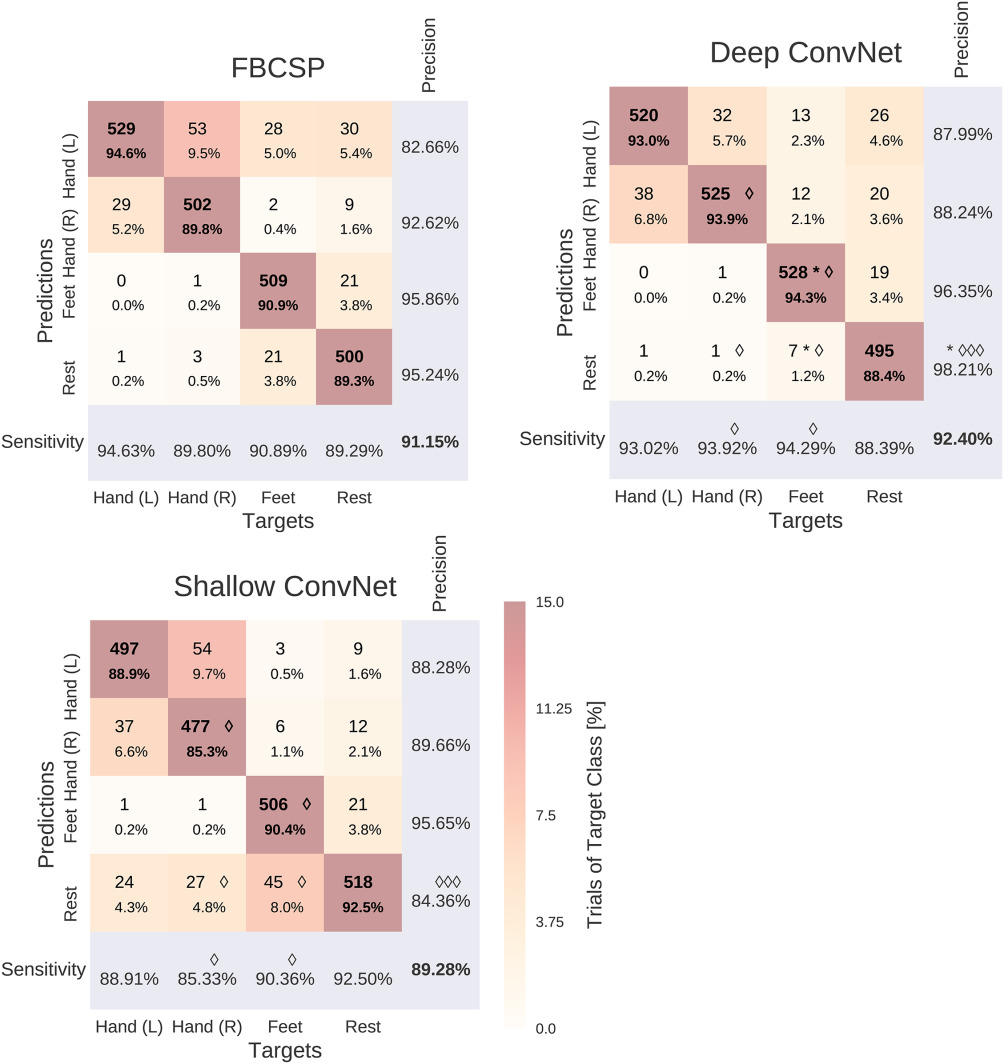
\includegraphics[width=0.9\linewidth]{images/Confusion_Mats.jpg}
    \caption[Confusion matrices for FBCSP- and ConvNet-based decoding]{
\textbf{Confusion matrices for FBCSP- and ConvNet-based decoding.}
Results are shown for the High-Gamma Dataset, on $0–f_\textrm{end}$
Hz. Each entry of row r and column c for upper-left 4×4-square: Number
of trials of target r predicted as class c (also written in percent of
all trials). Bold diagonal corresponds to correctly predicted trials of
the different classes. Percentages and colors indicate fraction of
trials of corresponding column (i.e.,
from trials of the corresponding target class). The lower-right
value corresponds to overall accuracy. Bottom row corresponds to
sensitivity
: $\frac{\mathrm{number\ of\ trials\ correctly\ predicted\ for\ 
class\ c}}{\mathrm{number\ of\ trials\ for\ class\ c}}$. Rightmost column corresponds to
precision: $\frac{\mathrm{number\ of\ trials\ correctly\ predicted\ for\ 
class\ r}}{\mathrm{number\ of\ trials\ predicted\ as\ class\ r}}$. Stars indicate statistically
significantly different values between ConvNet decoding and FBCSP, diamonds between the shallow and deep ConvNets. P\textless0.05: $\diamond$/*,
P\textless0.01: $\diamond\diamond$/**, P\textless0.001:
$\diamond\diamond\diamond$/***, Wilcoxon signed-rank test. Figure from
\citet{schirrmeisterdeephbm2017}.
}
\label{confusion-mat-figure}
\end{figure}



\begin{table}[htb]
\centering \footnotesize
\begin{tabular}{lllllll}\toprule
&
\tableheadline{\parbox{0.12\linewidth}{Hand (L)\\Hand (R)}} & 
\tableheadline{\parbox{0.12\linewidth}{Hand (L)\\Feet}} & 
\tableheadline{\parbox{0.12\linewidth}{Hand (L)\\Rest}} & 
\tableheadline{\parbox{0.12\linewidth}{Hand (R)\\Feet}} & 
\tableheadline{\parbox{0.12\linewidth}{Hand (R)\\Rest}} & 
\tableheadline{\parbox{0.05\linewidth}{Feet\\Rest}} \\\midrule
 FBCSP & 82 & 28 & 31 & 3 & 12 & 42 \\ 
 Deep & 70 & 13 & 27 & 13 & 21 & 26 \\ 
 Shallow & 99 & 3 & 34 & 5 & 37 & 73 \\ 
  \bottomrule
\hline
\end{tabular}
\caption[Decoding errors between class pairs]{\textbf{Decoding errors between class pairs.} Results for the High-Gamma Dataset.
Number of trials where one class  was mistaken for the
other for each decoding method, summed per class pair. The largest
number of errors was between Hand(L) and Hand (R) for all three
decoding methods, the second largest between Feet and Rest (on average
across the three decoding methods). Together, these two class pairs
accounted for more than 50\% of all errors for all three decoding
methods. In contrast, Hand (L and R) and Feet had a small number of
errors irrespective of the decoding method used.}
\label{hgd-class-mistakes-table} 
\end{table}

    Confusion matrices for the High-Gamma Dataset on 0--$f_{end}$ Hz were
very similar for FBCSP and both ConvNets (see
\Cref{confusion-mat-figure}). The majority of all mistakes
were due to discriminating between Hand (L) / Hand (R) and Feet / Rest,
see Table \Cref{hgd-class-mistakes-table}. Seven entries of
the confusion matrix had a statistically significant difference
(p\textless0.05, Wilcoxon signed-rank test) between the deep and the
shallow ConvNet, in all of them the deep ConvNet performed better. Only
two differences between the deep ConvNet and FBCSP were statistically
significant (p\textless0.05), none for the shallow ConvNet and FBCSP.
Confusion matrices for the BCI competition IV dataset 2a showed a larger
variability and hence a less consistent pattern, possibly because of the
much smaller number of trials.

\section{Residual ConvNets Can Be Competitive with Improved
Training}\label{residual-convnets-can-be-competitive-with-improved-training}


\begin{table}[htb]
    \myfloatalign
    \begin{tabularx}{\textwidth}{lllll}
    \toprule
        \tableheadlinewithwidth{0.25\textwidth}{Dataset} & \tableheadlinewithwidth{0.2\textwidth}{Frequency Range (Hz)} &
        \tableheadlinewithwidth{0.12\textwidth}{FBCSP}  & 
        \tableheadlinewithwidth{0.12\textwidth}{ResNet Before} & 
        \tableheadlinewithwidth{0.12\textwidth}{ResNet Now} 
        \\
        \midrule
        BCIC IV 2a & 0--38 & 68.0 & -0.3 & +3.7 \\
        BCIC IV 2a & 4--38 & 67.8 & -7.0* & -0.9 \\
        HGD & 0--125 & 91.2 & -2.3* & +1.1 \\
        HGD & 4--125 & 90.9 & -1.1 & 0.0 \\
        Combined & 0--$f_{end}$ & 82.1 & -1.1 & +2.2 \\
        Combined & 4--$f_{end}$ & 81.9 & -3.5* & -0.4 \\
        \bottomrule
    \end{tabularx}
    \caption[Residual ConvNet vs. FBCSP Accuracies]{
   \textbf{Residual ConvNet vs. FBCSP Accuracies.} Accuracies
and significance stars have same meaning as before.
    }  \label{residual-hgd-results}
\end{table}

In our original study, residual ConvNets had underperformed our FBCSP
baseline, in several settings even with statistical significance.
However, later investigations revealed that better weight
initializations, concretely scaling down the weight initialization more
strongly, can lead to improved results. In work done for this thesis, I
repeated the original experiments using our current decoding pipeline
with the residual ConvNets. \Cref{residual-hgd-results}
reports the original accuracies and the accuracies obtained with our
current codebase. Notably, residual ConvNets no longer substantially
underperform FBCSP, even slightly outperforming it in the setting
without highpass.


\section{Design Choices Affected Decoding Performance}\label{design-choices-results}



\begin{figure}[h!tb]
    \captionsetup[subfigure]{labelformat=empty}
    \myfloatalign
    \subfloat[]
    {
        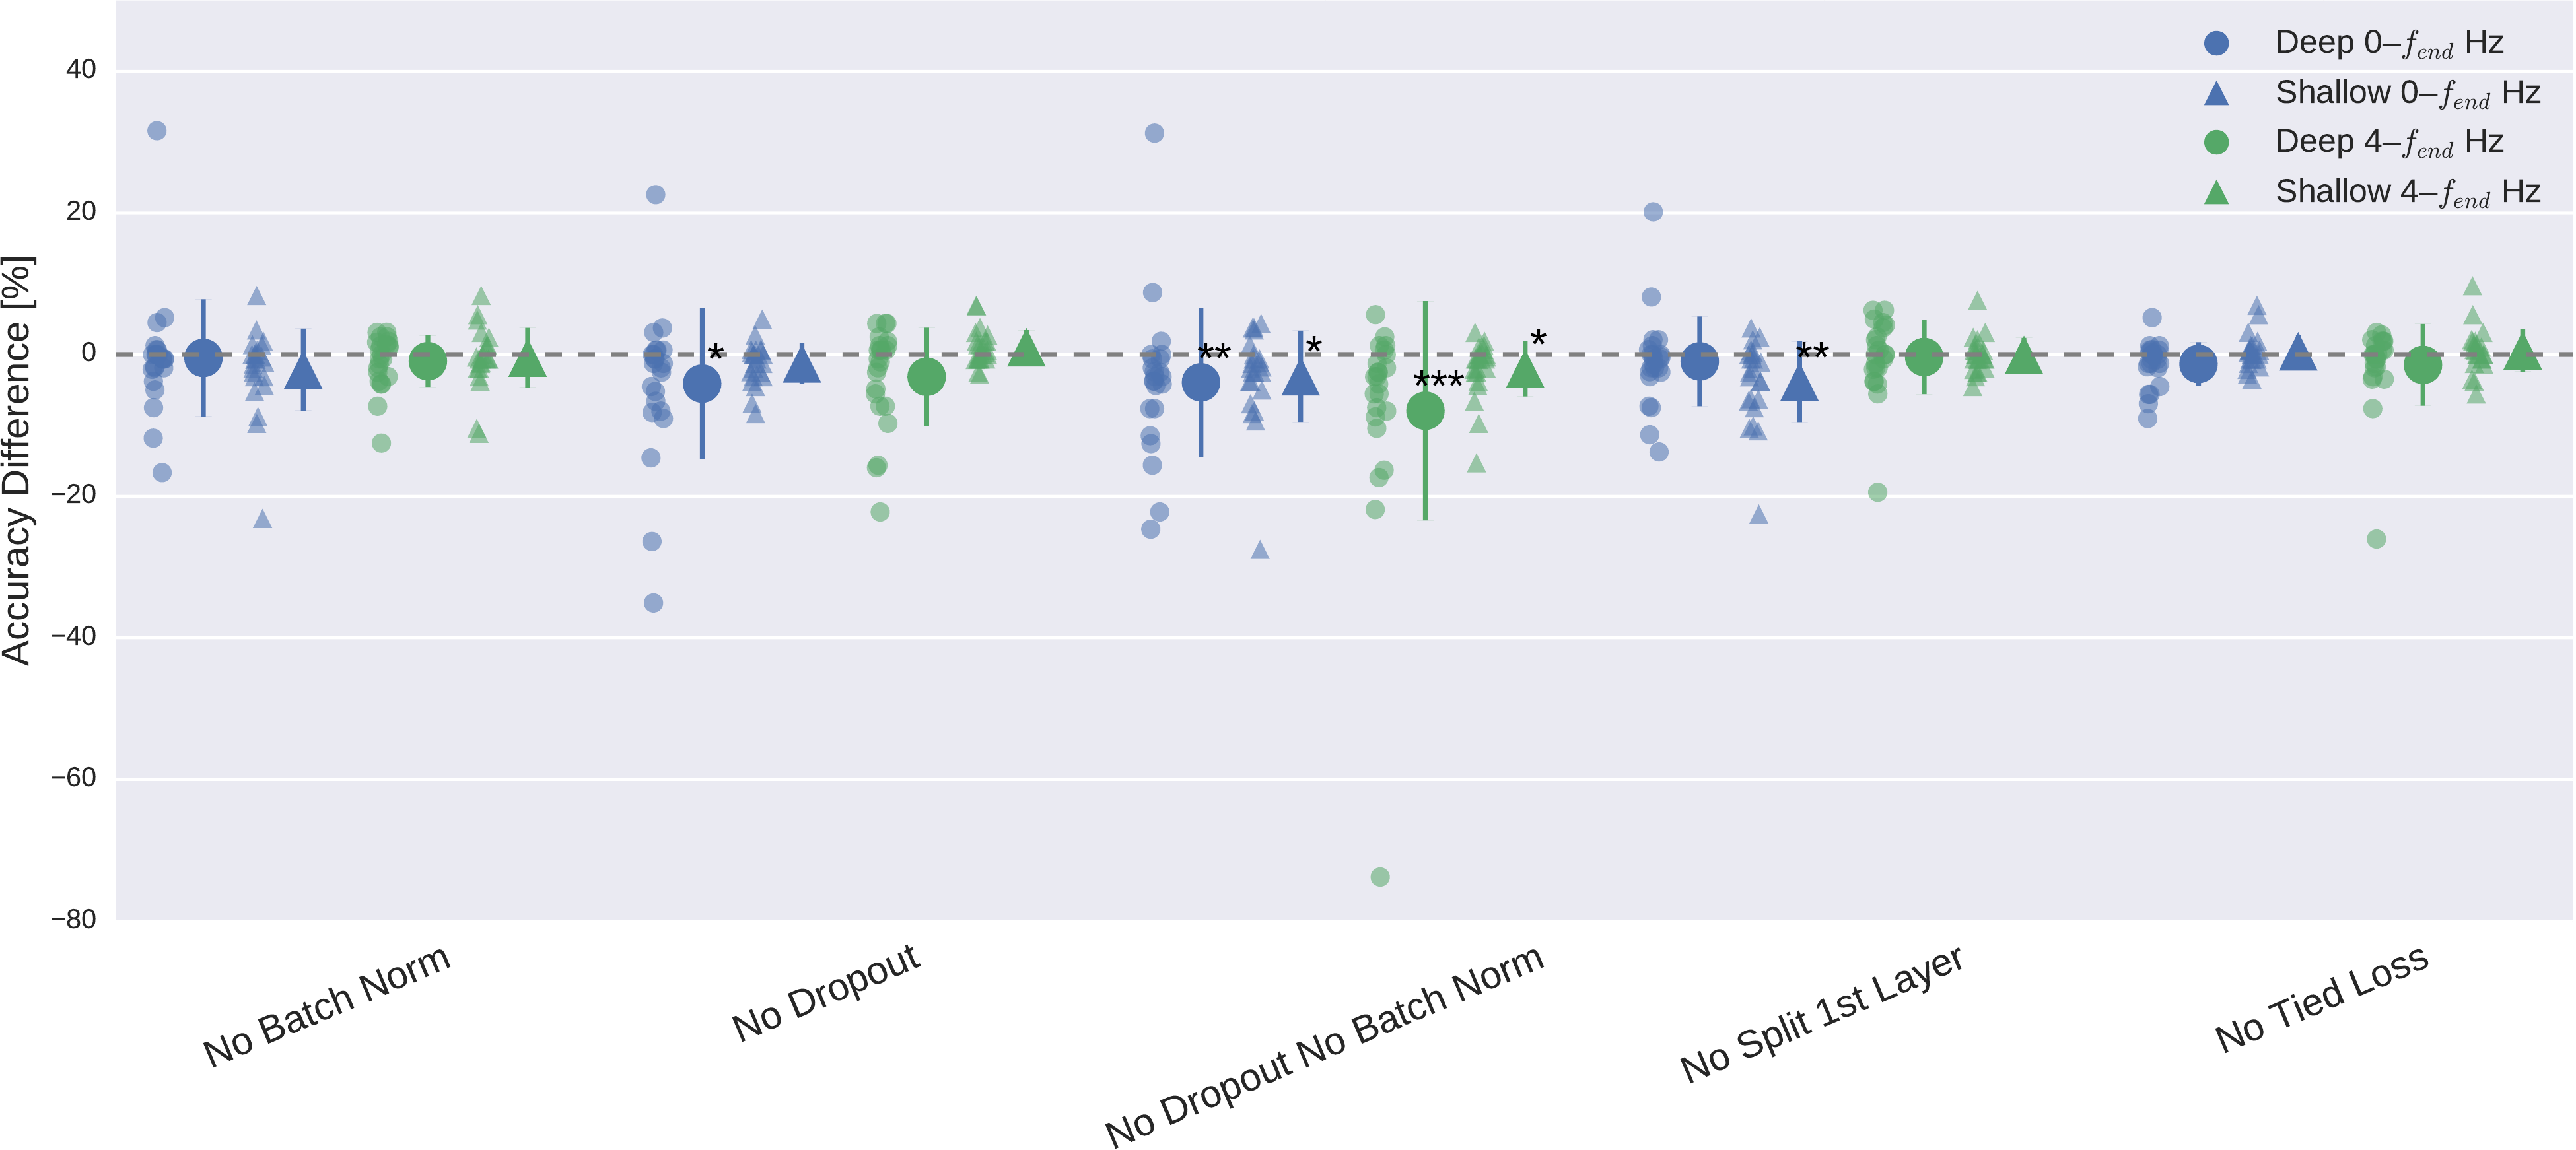
\includegraphics[width=0.9\linewidth]{images/Final_Comparison.ipynb.9.pdf-1.png} 
    } \\
    \vspace{-0.5cm}
    \subfloat[]
    {
    \label{design-choices-b-fig}
    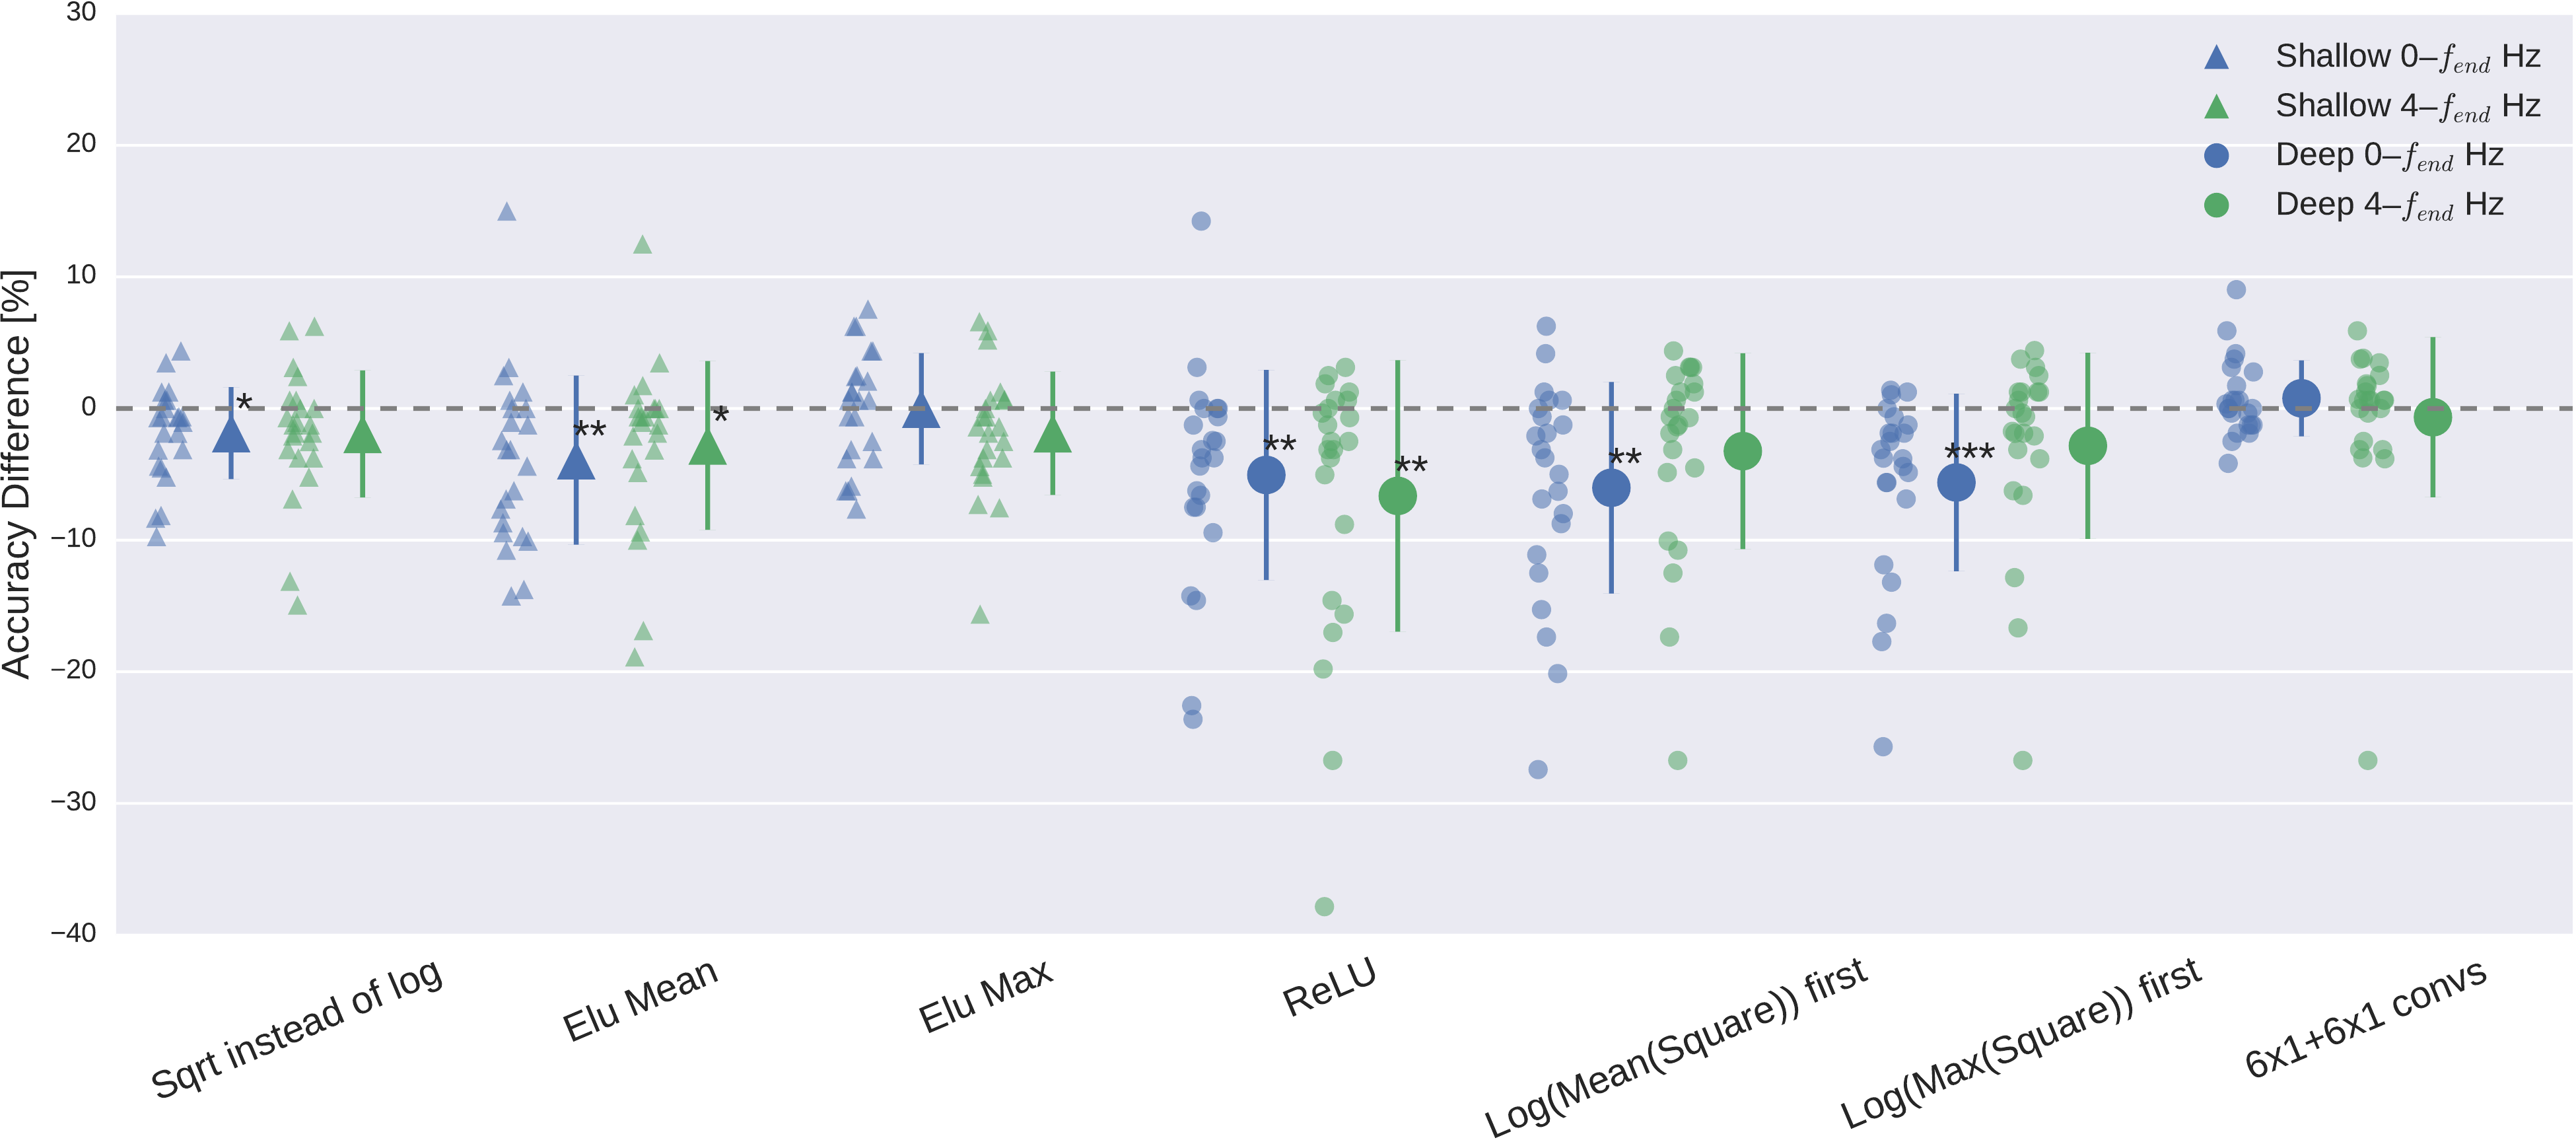
\includegraphics[width=0.9\linewidth]{images/Final_Comparison.ipynb.10.pdf-1.png}
    }
    \caption[Impact of ConvNet design choices on decoding accuracy]{
    \textbf{Impact of ConvNet design choices on decoding accuracy.} 
Accuracy differences of baseline and design choices on x-axis for the $0-f_\textrm{end}$ Hz and $4-f_\textrm{end}$ Hz datasets. 
Each small marker represents accuracy difference for one subject, and each larger marker represents mean accuracy difference across all subjects of both datasets. Bars: standard error of the differences across subjects. 
Stars indicate statistically significant differences to baseline (Wilcoxon signed-rank test, P < 0.05: $\diamond$\*, P < 0.01: $\diamond\diamond$\*\*, P < 0.001=\*\*\*). Top: Impact of design choices applicable to both ConvNets. 
All statistically significant differences were accuracy decreases from removing an aspect of our architecture.
Notably, there was a clear negative effect of removing both dropout and batch normalization. Bottom: Impact of different types of nonlinearities, pooling modes and filter sizes. Results are given independently for the deep ConvNet and the shallow ConvNet.
As before, all statistically significant differences were from accuracy decreases. Notably, replacing ELU by ReLU as nonlinearity led to decreases on both frequency ranges, which were both statistically significant. 
Figure from \citet{schirrmeisterdeephbm2017}.
}
\label{design-choices-fig}
\end{figure}

    Design choices substantially affected deep network accuracies on both
datasets, meaning BCI Competition IV 2a and the High Gamma Dataset.
Batch normalization and dropout significantly increased accuracies. This
became especially clear when omitting both simultaneously
\Cref{design-choices-fig}. Batch normalization provided a
larger accuracy increase for the shallow ConvNet, whereas dropout
provided a larger increase for the deep ConvNet. For both networks and
for both frequency bands, the only statistically significant accuracy
differences were accuracy decreases after removing dropout for the deep
ConvNet on $0-f\_\textrm{end}$ Hz data or removing batch
normalization and dropout for both networks and frequency ranges
($p<0.05$, Wilcoxon signed-rank test). Usage of tied loss did not
affect the accuracies very much, never yielding statistically
significant differences ($p>0.05$). Splitting the first layer into two
convolutions had the strongest accuracy increase on the
$0-f\_\textrm{end}$ Hz data for the shallow ConvNet, where it is also
the only statistically significant difference ($p<0.01$).

\section{Cropped Training Strategy Improved Deep ConvNet on Higher
Frequencies}\label{cropped-training-strategy-improved-deep-convnet-on-higher-frequencies}

\begin{figure}[htb]
    \myfloatalign
    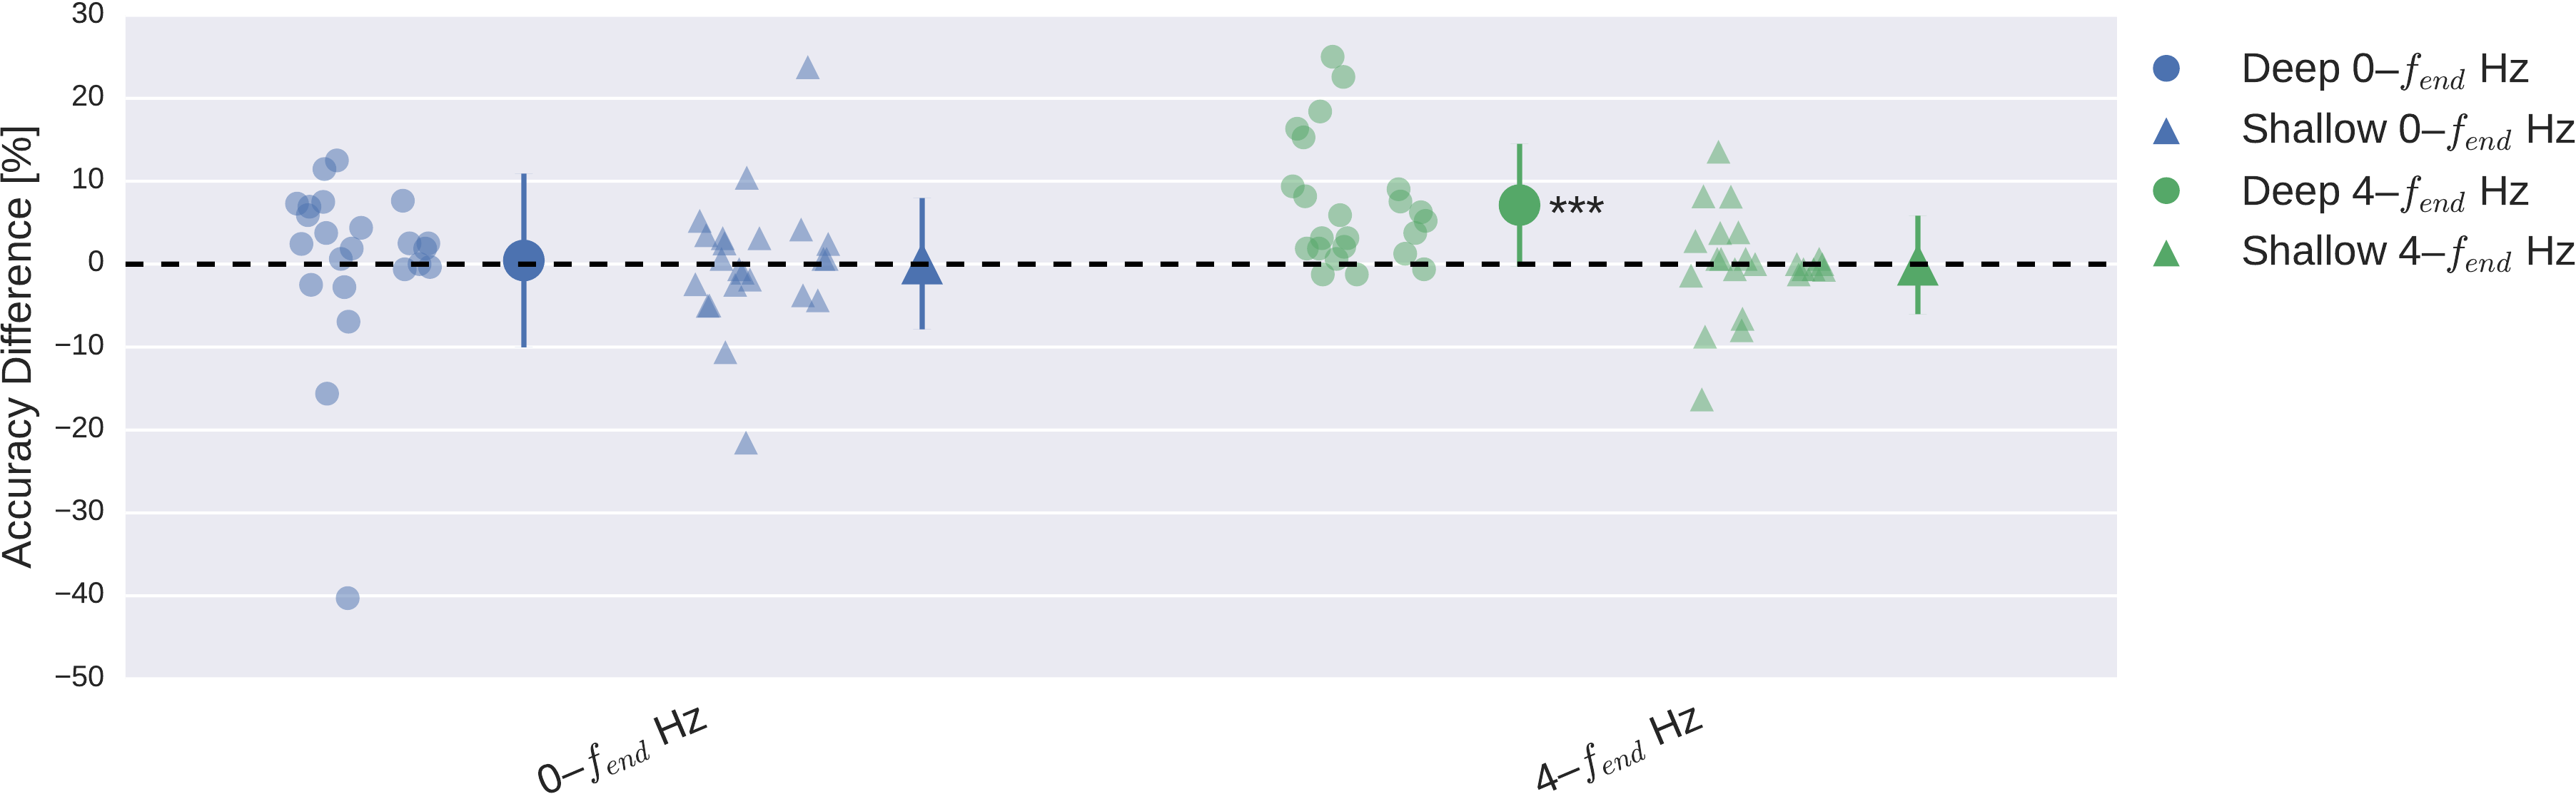
\includegraphics[width=1\linewidth]{images/Final_Comparison.ipynb.8.pdf-1.png}
    
    \caption[Impact of training strategy on decoding accuracy]{
\textbf{Impact of training strategy (cropped vs trial-wise training) on
accuracy.} Accuracy difference for both frequency ranges and both
ConvNets when using cropped training instead of trial-wise training.
Other conventions as in \Cref{design-choices-b-fig}. Cropped
training led to better accuracies for almost all subjects for the deep
ConvNet on the $4-f_\textrm{end}$-Hz frequency range. Figure from
\citet{schirrmeisterdeephbm2017}. 
}
\label{cropped-training-results-fig}
\end{figure}

    Cropped training increased accuracies statistically significantly for
the deep ConvNet on the $4-f_\textrm{end}$-Hz data (p\textless1e-5,
Wilcoxon signed-rank test, see
\Cref{cropped-training-results-fig}). In all other settings
($0-f_\textrm{end}$-Hz data, shallow ConvNet), the accuracy
differences were not statistically significant (p\textgreater0.1) and
showed a lot of variation between subjects.

\section{Results on BCI Competition IV
2b}\label{results-on-bci-competition-iv-2b}


\begin{table}[htb]
    \myfloatalign
    \begin{tabularx}{\textwidth}{lll}
    \toprule
        \tableheadlinewithwidth{0.2\textwidth}{FBCSP} & \tableheadlinewithwidth{0.2\textwidth}{Deep ConvNet} &
        \tableheadlinewithwidth{0.2\textwidth}{Shallow ConvNet} 
        \\
        \midrule
0.599 & -0.001 & +0.030 \\
        \bottomrule
    \end{tabularx}
    \caption[Kappa values on the BCIC IV 2b dataset]{
\textbf{Kappa values on the BCIC IV 2b dataset.} ConvNet
kappa values show the difference to the FBCSP kappa value.
    }  \label{bcic-iv-2b-results}
\end{table}


    To ensure that the results also generalize to further datasets and also
rule out hyperparameter overfitting, the FBCSP pipeline and the deep
network pipelines were applied with the exact same hyperparameters on
BCI Competition IV 2b. A few choices like the use of the decoding time
window had been done after already seeing results from the evaluation
sets of the High-Gamma dataset and the BCIC IV 2a dataset, hence it was
valuable to validate the results on the BCIC IV 2b dataset. Results in
\Cref{bcic-iv-2b-results} show that the networks perform as
good or better than FBCSP. Results on further datasets, also
non-movement-decoding datasets are presented in the next chapter
\Cref{task-related}.

\section{ConvNet-Independent
Visualizations}\label{convnet-independent-visualizations}



\begin{figure}[htb]
    \myfloatalign
    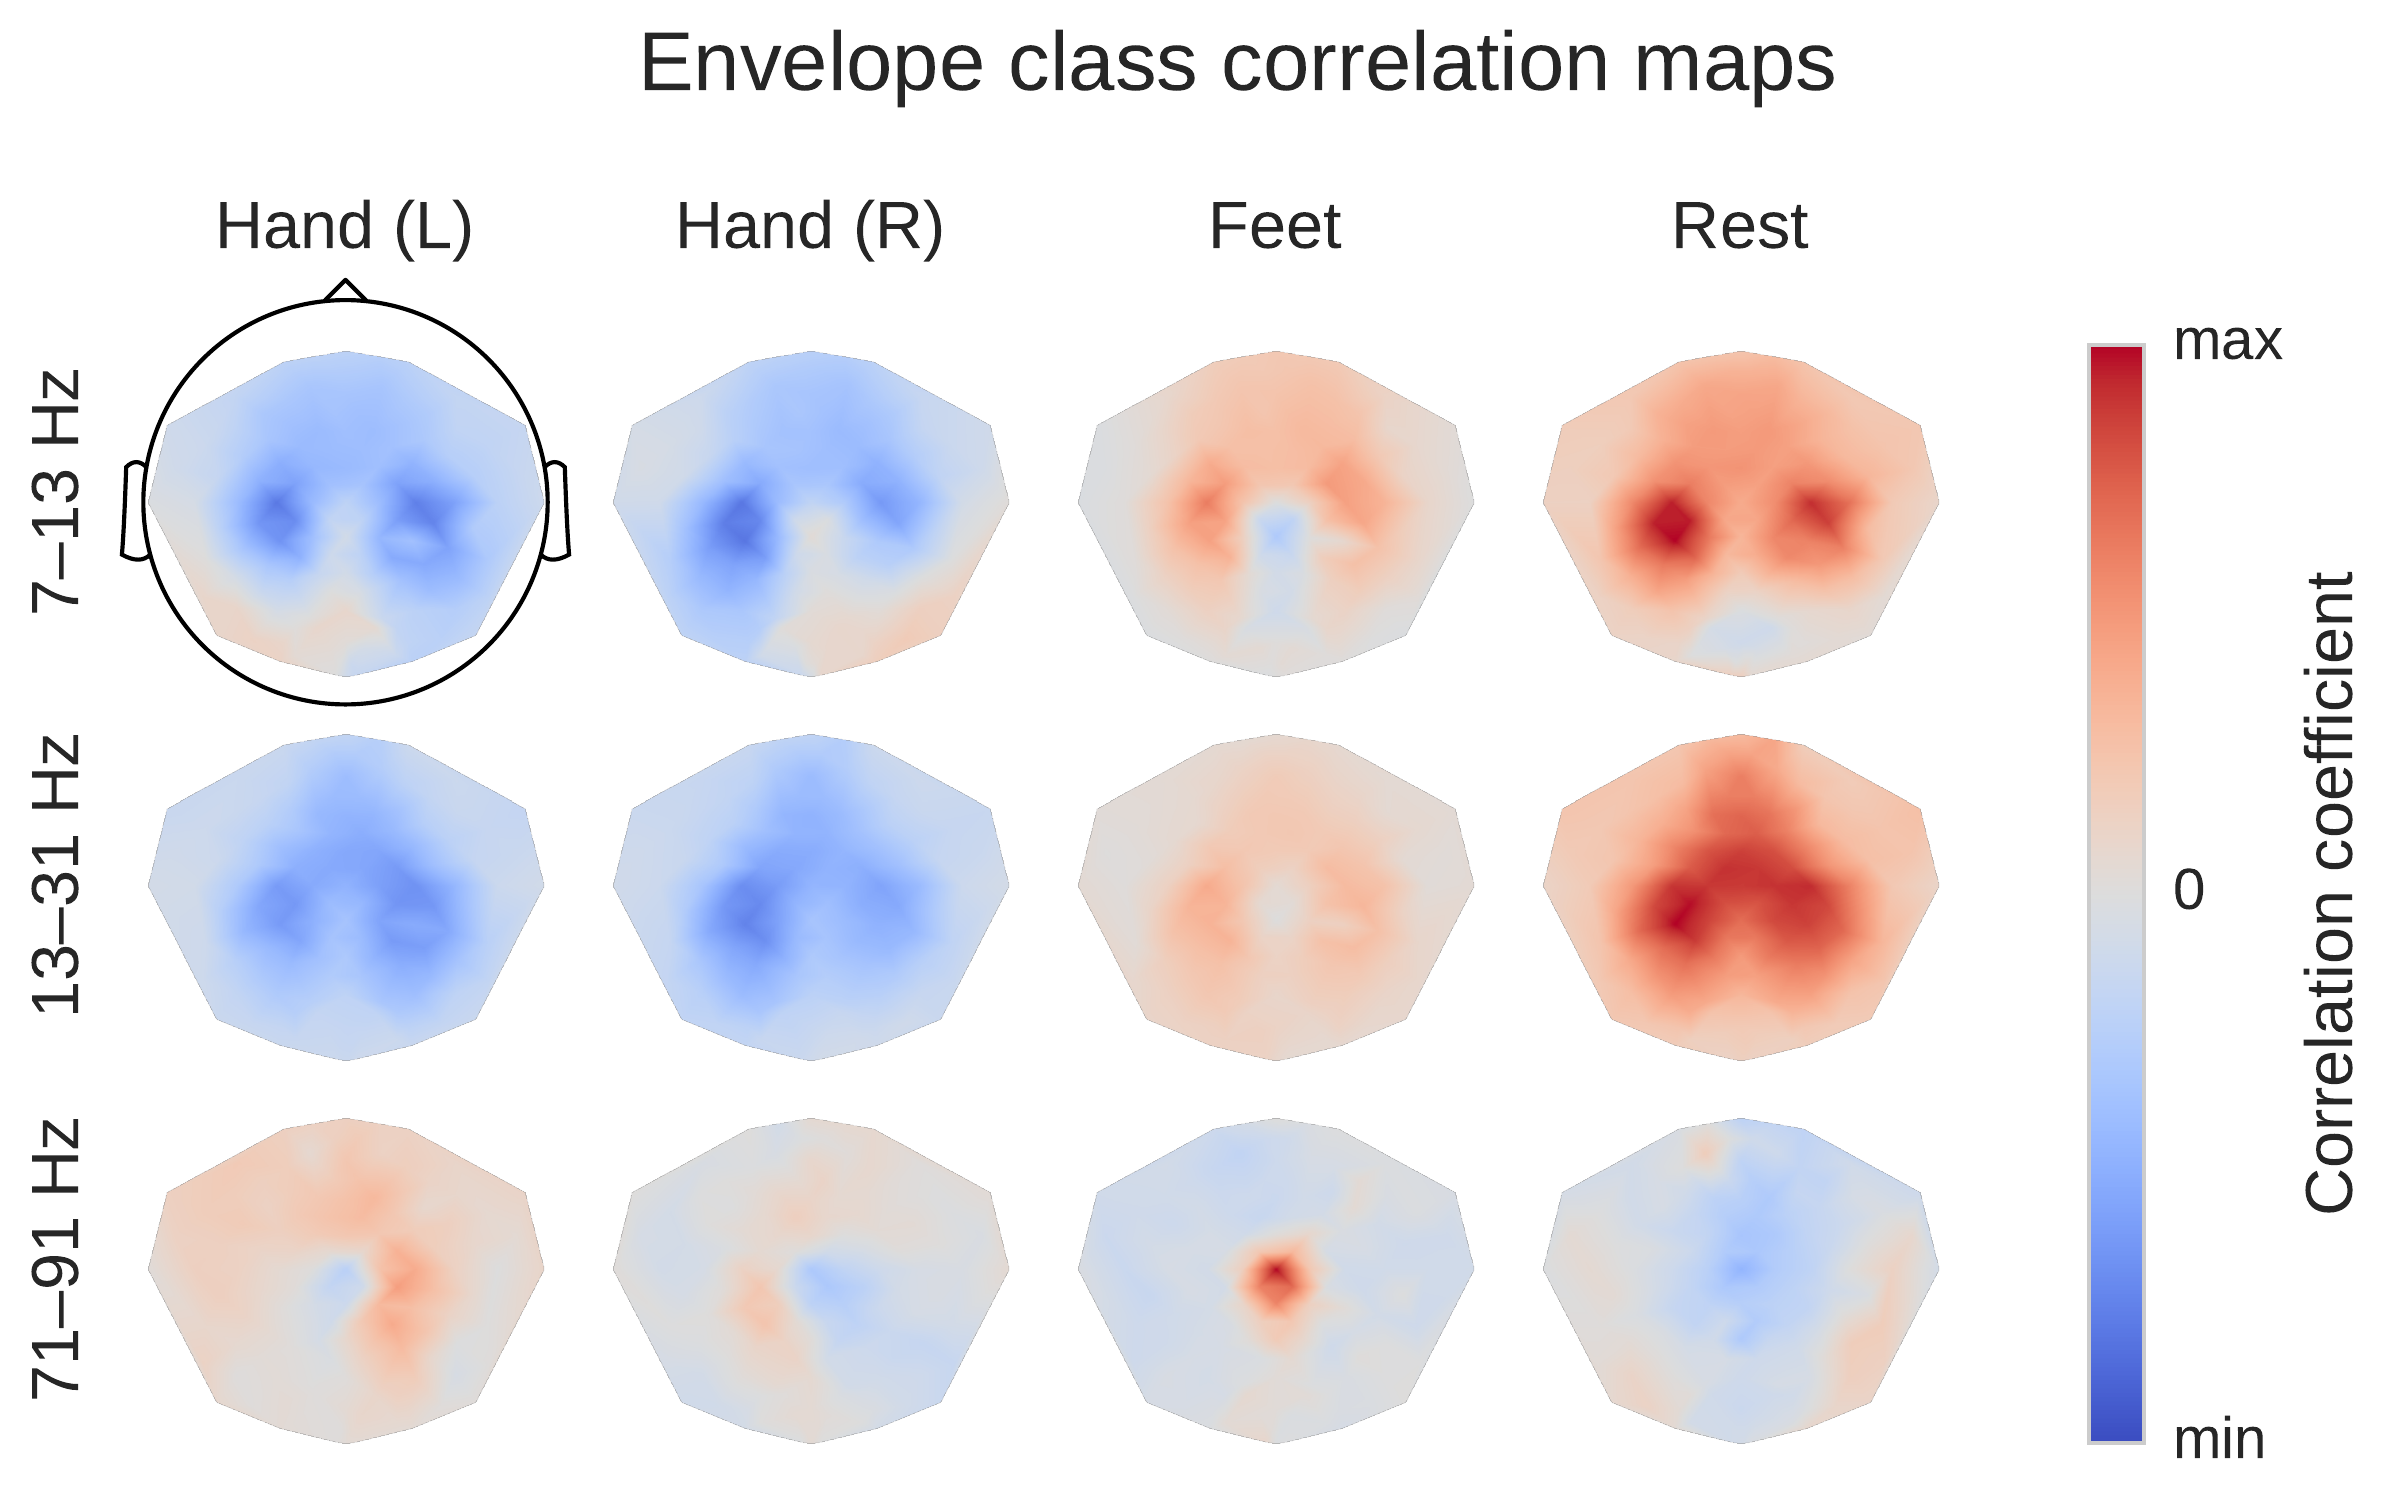
\includegraphics[width=1\linewidth]{images/Envelope_Correlations.ipynb.1.pdf-1.png}
    
    \caption[Envelope correlations on high-gamma dataset]{
\textbf{Average envelope correlations over subjects from the high-gamma dataset.} Colormaps are scaled per frequency band/row. This is a ConvNet-independent
visualization. Scalp plots show spatial distributions of class-related
spectral amplitude changes well in line with the literature. Figure from
\citet{schirrmeisterdeephbm2017}.
}
\label{envelope-class-fig}
\end{figure}


    Before moving to ConvNet visualization, we examined the spectral
amplitude changes associated with the different movement classes in the
alpha, beta and gamma frequency bands. For that, we first computed the
moving average of the squared envelope in narrow frequency bands via the
Hilbert transform as a measure of the power in those frequency bands.
Then we computed linear correlations of these moving averages with the
class label. This results in frequency-resolved envelope-class label
correlations.

We found the expected overall scalp topographies (see
\Cref{envelope-class-fig}) to show physiologically plausible
patterns. For example, for the alpha (7--13 Hz) frequency band, there
was a class-related power decrease (anti-correlation in the
class-envelope correlations) in the left and right pericentral regions
with respect to the hand classes, stronger contralaterally to the side
of the hand movement , i.e., the regions with pronounced power decreases
lie around the primary sensorimotor hand representation areas. For the
feet class, there was a power decrease located around the vertex, i.e.,
approx. above the primary motor foot area. As expected, opposite changes
(power increases) with a similar topography were visible for the gamma
band (71--91 Hz).

\section{Amplitude Perturbation
Visualizations}\label{amplitude-perturbation-visualizations}



\begin{figure}[t!hb]
    \myfloatalign
    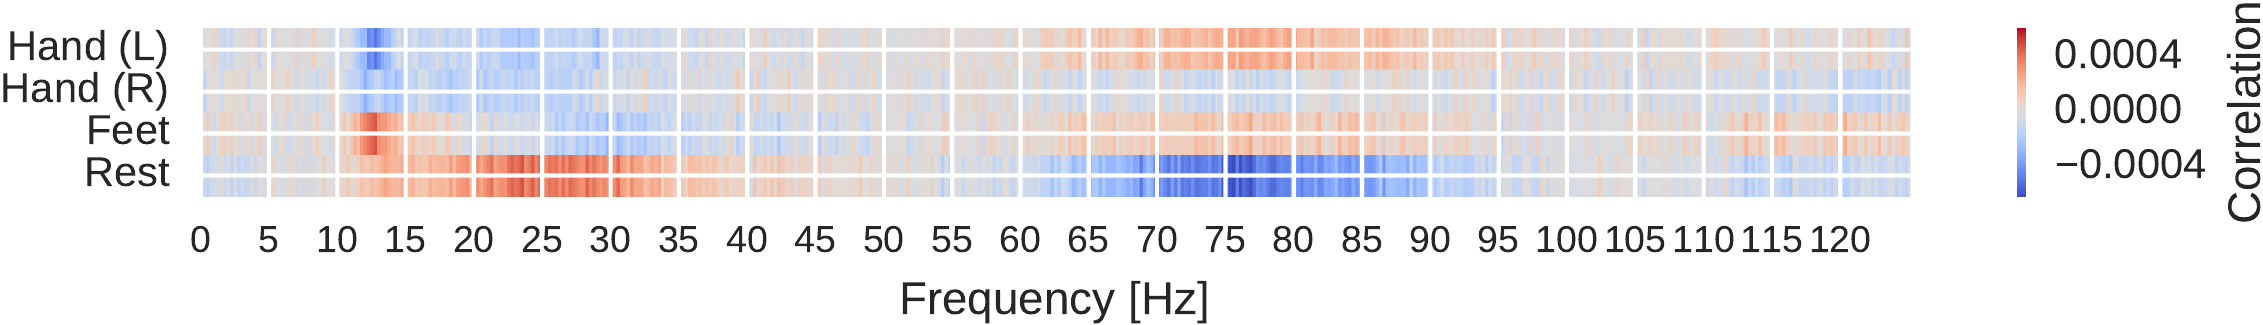
\includegraphics[width=1\linewidth]{images/Bandpower_Perturbation.ipynb.0.pdf-1.png}
    
    \caption[Per-class amplitude perturbation correlation profiles on high-gamma dataset]{
\textbf{Input-perturbation network-prediction correlations for all
frequencies for the deep ConvNet, per class.} Plausible correlations,
for example, rest positively, other classes negatively correlated with
the amplitude changes in frequency range from 20 to 30 Hz. Figure from
\citet{schirrmeisterdeephbm2017}.
}
\label{bandpower-perturbation-per-class-fig}
\end{figure}


\begin{figure}[htb]
    \myfloatalign
    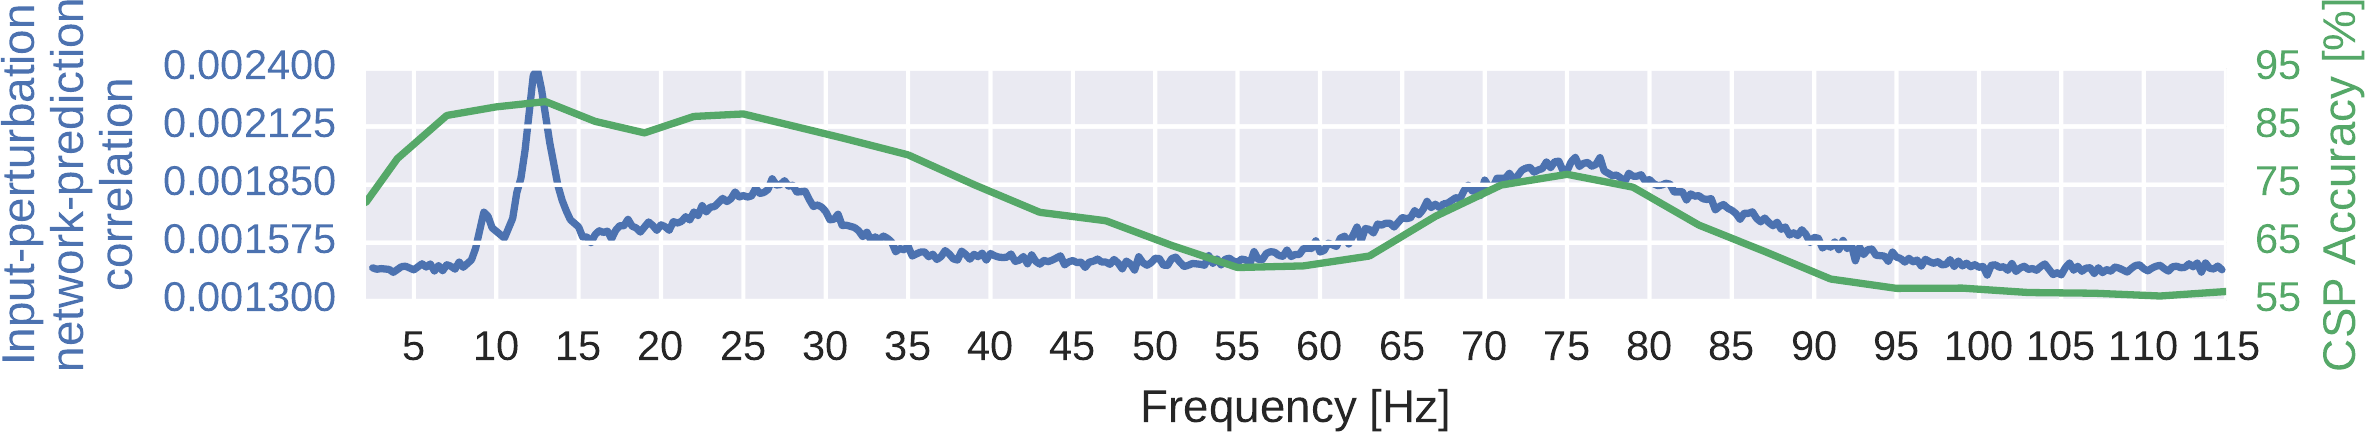
\includegraphics[width=1\linewidth]{images/Bandpower_Perturbation.ipynb.12.pdf-1.png}
    
    \caption[Overall amplitude perturbation correlation profile on high-gamma dataset]{
\textbf{Absolute input-perturbation network-prediction correlation
frequency profile for the deep ConvNet.} Mean absolute correlation value
across classes. CSP binary decoding accuracies for different frequency
bands for comparison, averaged across subjects and class pairs. Peaks in
alpha, beta, and gamma band for input-perturbation network-prediction
correlations and CSP accuracies. Figure from
\citet{schirrmeisterdeephbm2017}.
}
\label{bandpower-overall-fig}
\end{figure}

Our amplitude perturbation visualizations show that the network have
learned to extract commonly used spectral amplitude features.We show
three visualizations extracted from input-perturbation
network-prediction correlations, the first two to show the frequency
profile of the causal effects, the third to show their topography. Thus,
first, we computed the mean across electrodes for each class separately
to show correlations between classes and frequency bands. We see
plausible results, for example, for the rest class, positive
correlations in the alpha and beta bands and negative correlations in
the gamma band in
\Cref{bandpower-perturbation-per-class-fig}.



    Then, second, by taking the mean of the absolute values both over all
classes and electrodes, we computed a general frequency profile. This
showed clear peaks in the alpha, beta, and gamma bands
(\Cref{bandpower-overall-fig}). Similar peaks were seen in
the means of the CSP binary decoding accuracies for the same frequency
range.


\begin{figure}[htb]
    \myfloatalign
    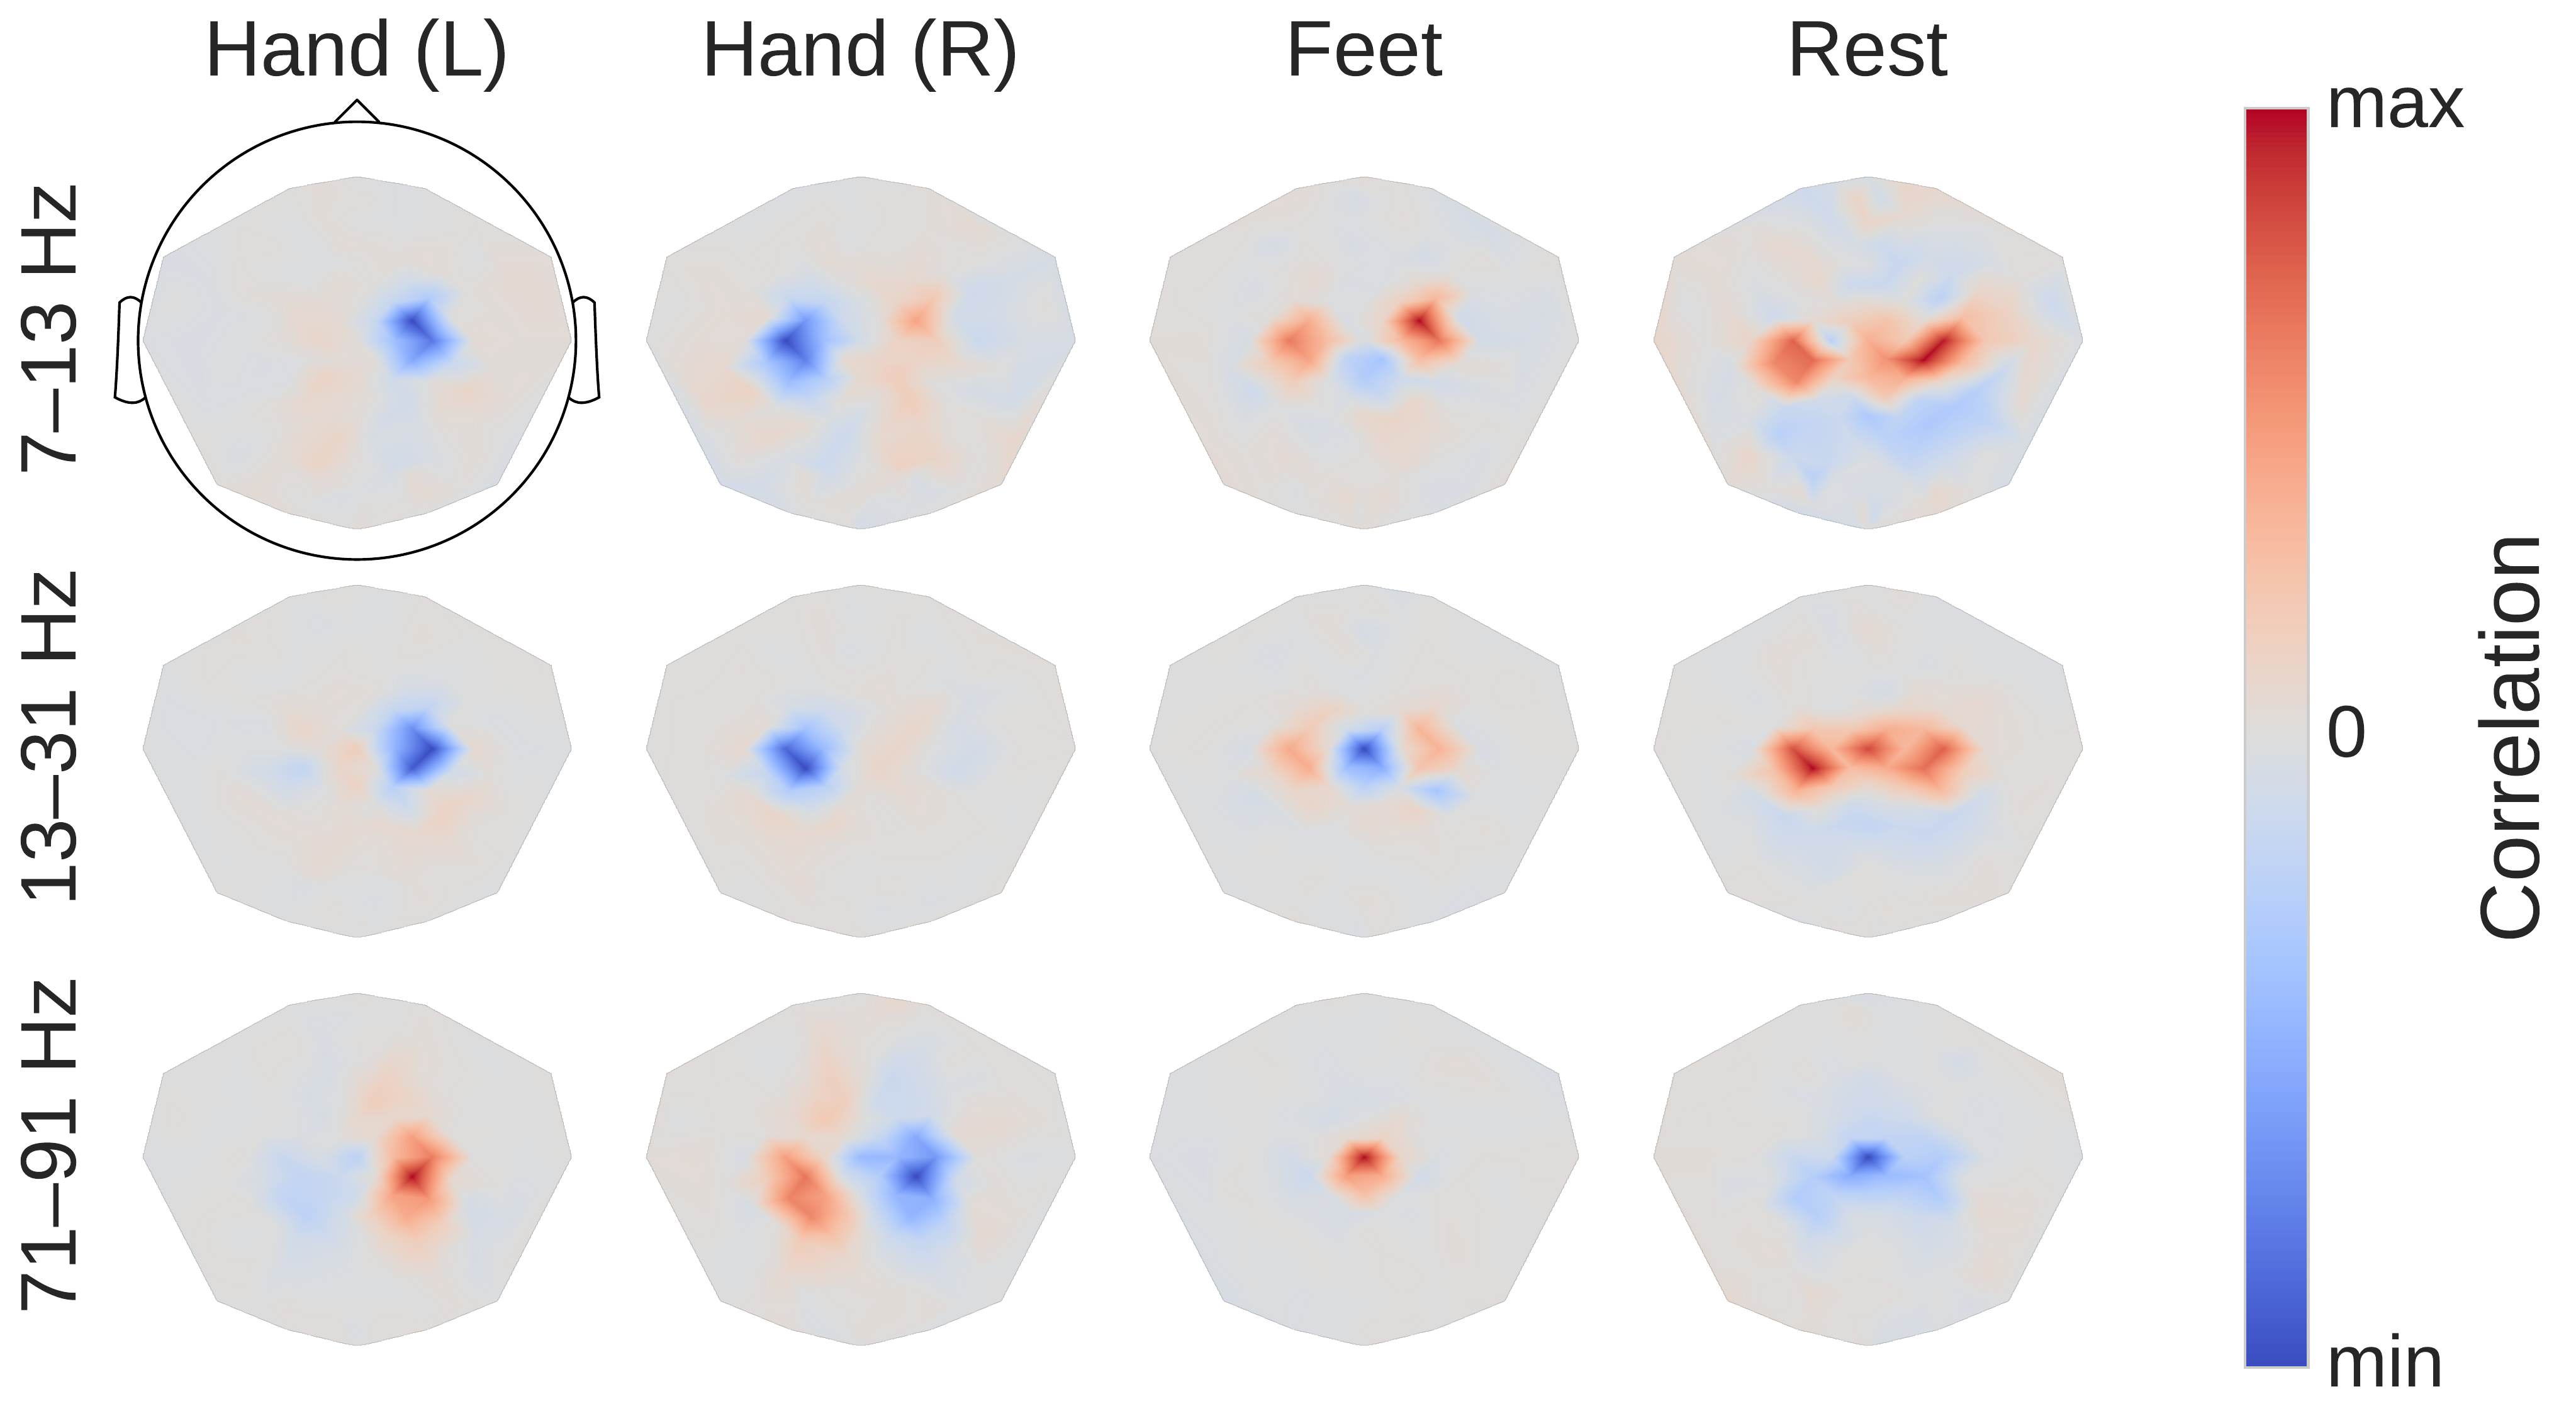
\includegraphics[width=1\linewidth]{images/Bandpower_Perturbation.ipynb.3.pdf-1.png}
    
    \caption[Amplitude perturbation correlation scalp plots on high-gamma dataset]{
\textbf{Input-perturbation network-prediction correlation maps for the
deep ConvNet.} Correlation of class predictions and amplitude changes.
Averaged over all subjects of the High-Gamma Dataset. Colormaps are
scaled per scalp plot. Plausible scalp maps for all frequency bands, for
example, contralateral positive correlations for the hand classes in the
gamma band. Figure from \citet{schirrmeisterdeephbm2017}.
}
\label{bandpower-perturbation-topo-fig}
\end{figure}




    Third, scalp maps of the input-perturbation effects on network
predictions for the different frequency bands, as shown in
\Cref{bandpower-perturbation-topo-fig}, show spatial
distributions expected for motor tasks in the alpha, beta and --- for
the first time for such a noninvasive EEG decoding visualization --- for
the high gamma band. These scalp maps directly reflect the behavior of
the ConvNets and one needs to be careful when making inferences about
the data from them. For example, the positive correlation on the right
side of the scalp for the Hand (R) class in the alpha band only means
the ConvNet increased its prediction when the amplitude at these
electrodes was increased independently of other frequency bands and
electrodes. It does not imply that there was an increase of amplitude
for the right hand class in the data. Rather, this correlation could be
explained by the ConvNet reducing common noise between both locations,
for more explanations of these effects in case of linear models, see
\Cref{perturbation-visualization-interpretation} and
\cite{haufe_interpretation_2014}. Nevertheless, for the
first time in noninvasive EEG, these maps clearly revealed the global
somatotopic organization of causal contributions of motor cortical gamma
band activity to decoding right and left hand and foot movements.
Interestingly, these maps revealed highly focalized patterns,
particularly during hand movement in the gamma frequency range
(\Cref{bandpower-perturbation-topo-fig}, first plots in last
row), in contrast to the more diffuse patterns in the conventional
task-related spectral analysis as shown in
\Cref{envelope-class-fig}.

\section{Internal Representations of Amplitude and
Phase}\label{internal-representations-of-amplitude-and-phase}

\begin{figure}[htb]
    \myfloatalign
    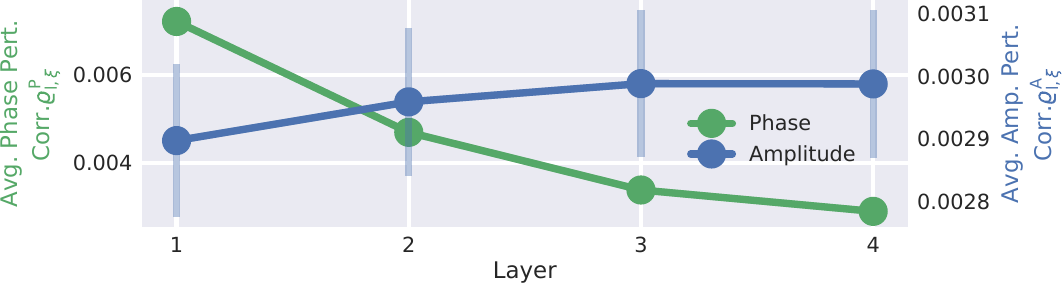
\includegraphics[width=1\linewidth]{images/PhaseAmpDev_.pdf-1.png}
    
    \caption[Mean phase and amplitude perturbation correlations over layers]{
\textbf{Mean phase and amplitude perturbation correlations over layers.}
Curves show mean perturbation correlation over all frequencies for each
layer. Scales are different and written on the left and right y-axes.
The error bars show the standard error over the subjects. Standard
errors for phase and amplitude are similar, but much higher relatively
in the amplitude correlation scale and therefore only visible there. In
their respective scale, curves show a clearly inverse behavior over the
layers with increasing amplitude correlations and decreasing phase
correlations. Figure from \citet{hartmann2018hierarchical}.
}
\label{phase-amp-dev-layer-fig}
\end{figure}


\begin{figure}[htb]
    \myfloatalign
    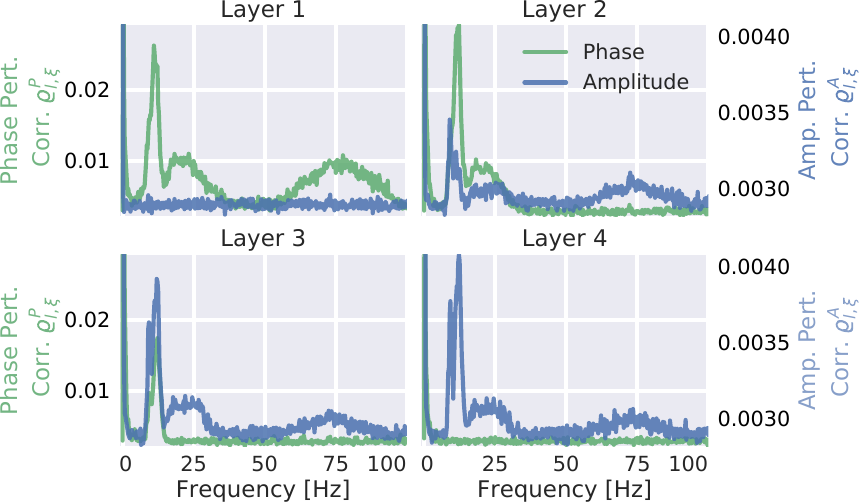
\includegraphics[width=1\linewidth]{images/PhaseAmp.pdf-1.png}
    
    \caption[Mean of absolute phase and amplitude perturbation correlations
for individual frequencies]{
\textbf{Mean of absolute phase and amplitude perturbation correlations
for individual frequencies.} The two correlation types have different
scales, denoted by the left and right y-axis. As in
\Cref{phase-amp-dev-layer-fig}, a clearly inverse relation
between amplitude and phase correlations is visible. This visualization
additionally showed that alpha (7-13 Hz), beta (13-30 Hz), and high
gamma (50-100 Hz) frequency ranges each have a specific layer in which
their phase correlation vanishes and their amplitude correlation
saturates (high gamma in layer 2, beta in layer 3, and alpha in layer
4). Figure from \citet{hartmann2018hierarchical}.
}
\label{phase-amp-layer-fig}
\end{figure}


    The perturbation analysis showed that the earlier layers represent more
phase-specific features than later layers, while the later layers
represent more phase-invariant amplitude features than the early layers.
\Cref{phase-amp-dev-layer-fig} shows the average absolute
phase perturbation correlation and amplitude perturbation correlation
over the 4 convolutional layers. The figure shows a clearly opposing
development of their respective average values across layers, with
increasing amplitude perturbation correlations and decreasing phase
perturbation correlations.

The perturbation correlations for individual frequencies showed a strong
phase perturbation correlation in the earlier layers 1 and 2 to phases
in the alpha, beta, and high gamma range (see
\Cref{phase-amp-layer-fig} ). The overall phase perturbation
correlation was highest in layer 1 and gradually became lower over
layers 2, 3, and 4. Interestingly, for each frequency band (alpha, beta,
and high gamma), there was one specific layer in which the phase
perturbation correlations vanished completely. Phase perturbation
correlations for high gamma vanished in layer 2, correlations for beta
vanished in layer 3, and correlations for alpha vanished in layer 4.
This vanishing of phase correlations for high gamma in layer 2 could be
observed in all subjects. For 4 subjects, alpha did already vanish
together with beta in layer 3.

An opposite behavior could be observed for amplitude correlations.
Notable phase insensitive amplitude perturbation correlations are only
emerging in layer 2. Amplitude correlations of individual frequency
bands peaked and saturated in the same layers in which the phase
correlation vanished: High gamma amplitude perturbation correlation
saturated in layer 2, beta in layer 3, and alpha in layer 4.

A potential underlying reason may be the use of max pooling with stride
3 after layers 1,2 and 3. The resulting temporal frequency resolutions
of the intermediate representations when only taking into account the
pooling strides are $\frac{250 \textrm{Hz}}{3} \approx 83\textrm{Hz}$,
$\frac{250 \textrm{Hz}}{3^2} \approx 28\textrm{Hz}$ and
$\frac{250 \textrm{Hz}}{3^3} \approx 9\textrm{Hz}$. The corresponding
Nyquist frequencies of approximately $41.5\textrm{Hz}$,
$14\textrm{Hz}$ and $4.5\textrm{Hz}$ seem to correspond to frequency
cutoffs above which the network is no longer phase-sensitive. However,
note that the network is in principle capable of retaining phase
sensitivity even in the presence of max pooling by shifting temporal
information to its channel dimension.

\section{Maximally Activating
Units}\label{maximally-activating-units}



\begin{figure}[h!tb]
    \captionsetup[subfigure]{labelformat=empty}
    \myfloatalign
    \subfloat[]
    {
    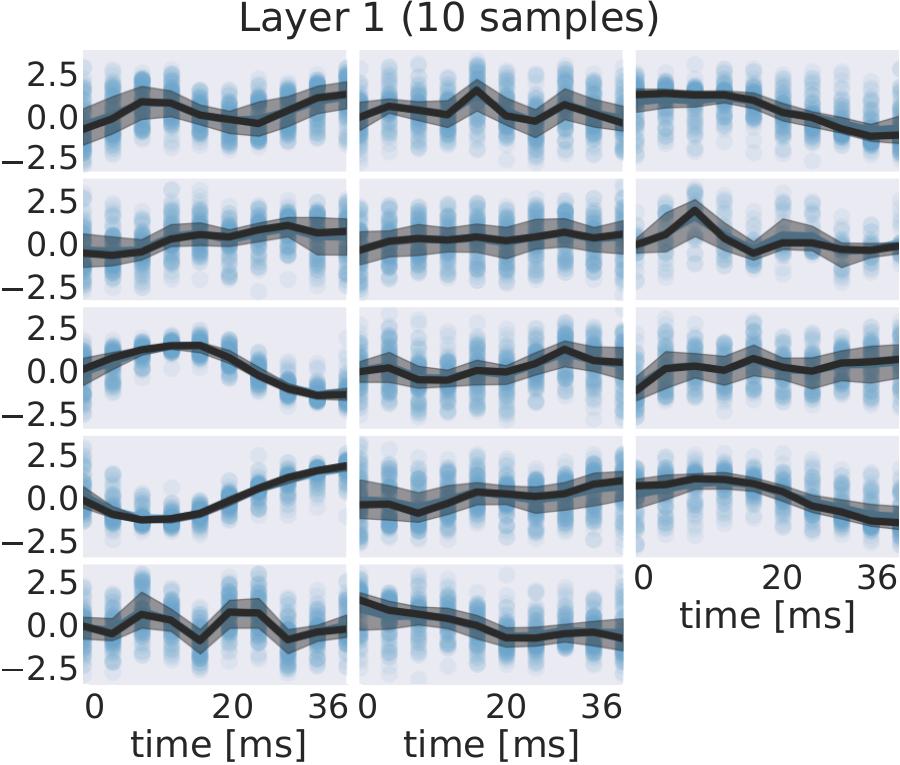
\includegraphics[width=.45\linewidth]{images/Inputs1_struct.pdf-1.png}} \quad
    \subfloat[] 
    {\
        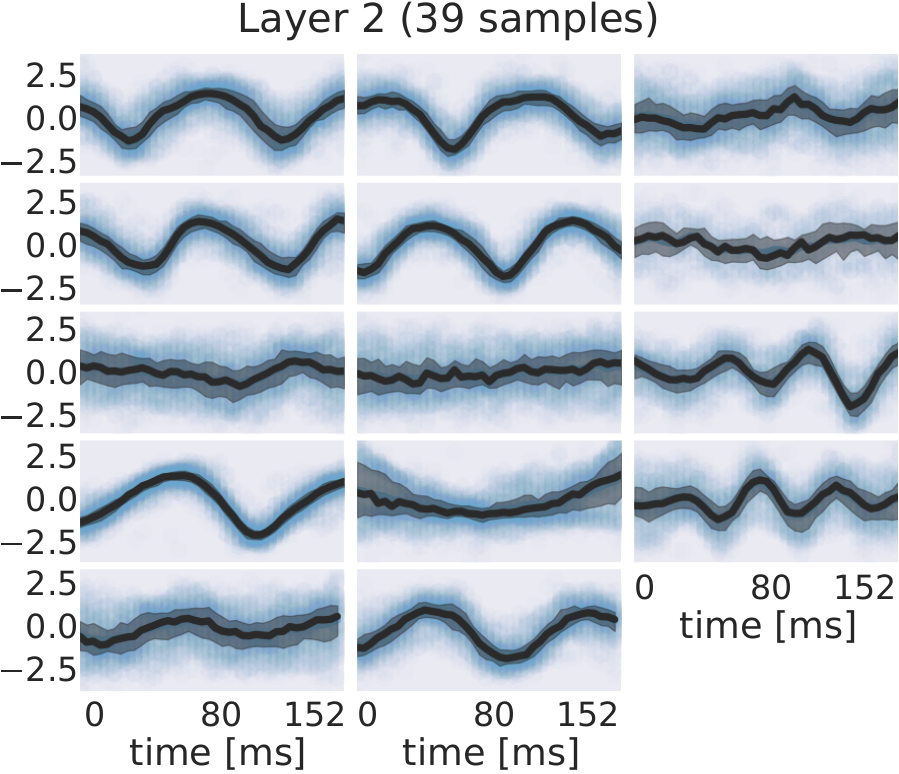
\includegraphics[width=.45\linewidth]{images/Inputs2_struct.pdf-1.png}} \\
    \subfloat[]
    {
    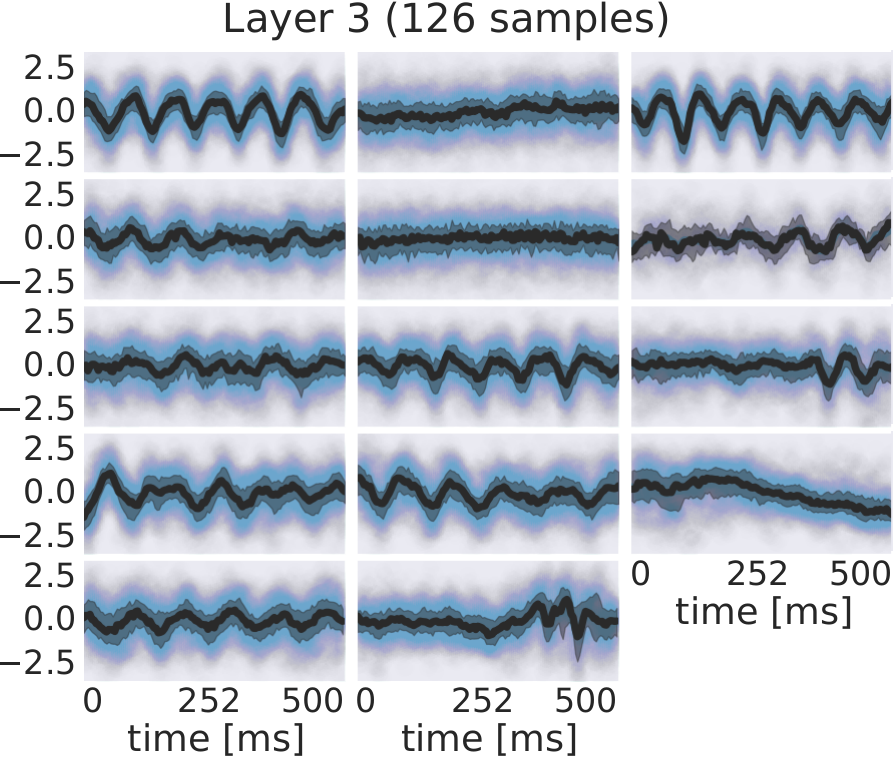
\includegraphics[width=.45\linewidth]{images/Inputs3_struct.pdf-1.png}} \quad
    \subfloat[]
    {
        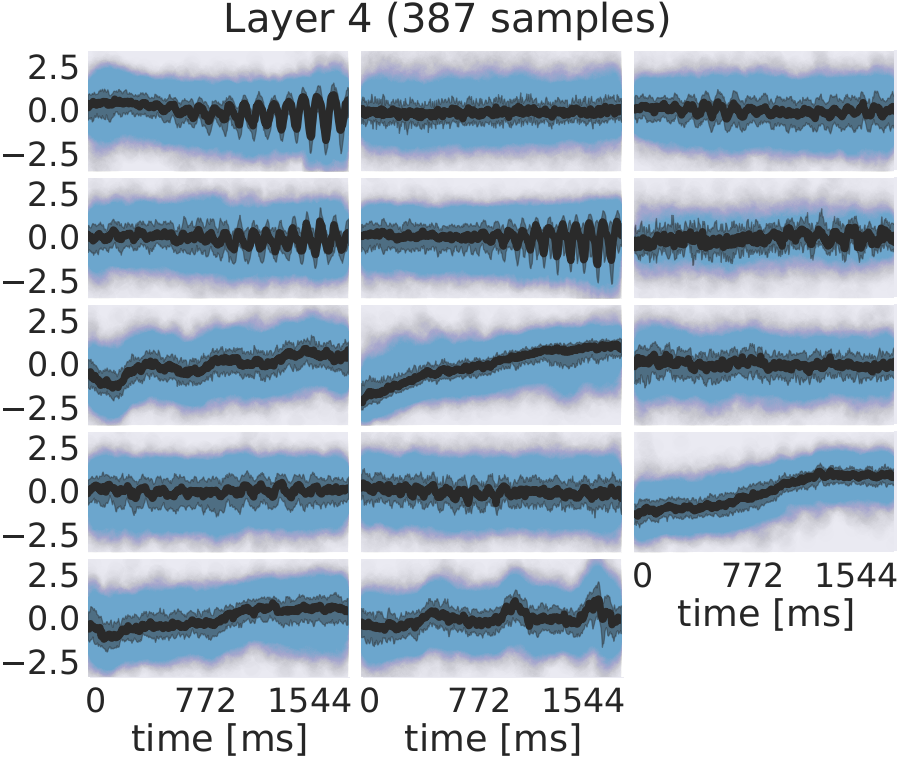
\includegraphics[width=.45\linewidth]{images/Inputs4_struct.pdf-1.png}} \\
    \caption[EEG signals in most-activating windows. per-electrode class prototypes]{
\textbf{EEG signals in most-activating input windows.} Taken from one randomly sampled filter in each layer for each subject. Blue points are the standard scores of all most-activating input windows for a filter. Their median is shown in black and the interquartile range as a gray shaded area. Medians in earlier layers often resemble parts of or complete sinusoids while medians in later layers resemble more complex
patterns. Figure from \citet{hartmann2018hierarchical}. 
    }\label{maximally-activating-units-fig}
\end{figure}



    In addition to examining how the individual layers respond to
frequency-specific phase and amplitude, we were also interested in other
characteristic features that might be learned by filters. To investigate
other features than frequency-specific phase or amplitude of sinusoidal
signals, we visually inspected the most-activating input windows of a
filter and their median values for each timepoint.
\Cref{maximally-activating-units-fig} shows the
most-activating input windows of one randomly sampled filter for each
subject and layer. We show each such set of most activating input
windows here at a representative electrode.
% 
For several filters, a clearly defined structure was present in the
median. The median plots for layer 1 show several examples of sinusoidal
shapes in different frequencies. Medians of higher frequencies were
sharper and the variance across input windows is larger. Medians of
layer 2 revealed several smooth alpha sinusoids, but also examples of
beta waves. In addition to that, there were some flat medians without an
easily interpretable periodicity or other temporal structure. In layer
3, there were mostly examples for alpha waves. For some medians in layer
4, more complex temporal patterns emerged. Those medians were relatively
flat at the beginning of the input windows, but showed an oscillatory
pattern with increasing amplitude in the later parts of the input
windows. Also, the oscillatory patterns in some examples resembled mu
waves more closely than pure sinusoids. Such patterns were found in
several subjects.

\section{Braindecode}\label{braindecode}

Work performed for this study also later led to the creation of the
open-source EEG deep learning library Braindecode, now with
contributions from multiple research groups and available at
\url{https://github.com/braindecode/braindecode/}.

\begin{openbox}
\item How well do ConvNets perform on other decoding tasks?
\item Do they work on tasks where oscillatory features are less important?
\item Do they work on non-trial based tasks like decoding pathology?
\end{openbox}

%************************************************
\chapter{Generalization to Other Tasks}\label{task-related}
%**************************************

\begin{startbox}{Our architectures generalize well to a wide variety of decoding tasks}
 \item Perform similar or better than common feature-based algorithms on mental imageries, error decoding, auditory evoked potentials
\item Also perform well on intracranial EEG
\item Deep networks performs a bit better than shallow network on average across tasks
\item EEGNet architecture developed by others also performs well
\item Networks can be used in an online BCI scenario
\end{startbox}



    After our initial work designing and evaluating convolutional neural
networks for movement decoding from EEG, we evaluated the resulting
networks on a wide variety of other EEG decoding tasks found that they
generalize well to a large number of settings such as error-related
decoding, online BCI control or auditory evoked potentials and also work
on intracranial EEG. 

Text and content condensed from a number of
publications, namely \citet{schirrmeisterdeephbm2017},
\citet{volker2018deep}, \citet{burget2017acting},
\citet{volker2018intracranial},
\citet{behncke2018cross}, \citet{wangsheep} and
\citet{heilmeyer2018large}. In all of these works except
\citet{schirrmeisterdeephbm2017}, I was not the main
contributor, I assisted in adapting the code and training for the
various settings and helped in the writing process.

\section{Decoding Different Mental
Imageries}\label{decoding-different-mental-imageries}


\begin{table}[htb]
    \myfloatalign
    \begin{tabularx}{\textwidth}{lll}
    \toprule
        \tableheadlinewithwidth{0.1\textwidth}{FBCSP} &
        \tableheadlinewithwidth{0.25\textwidth}{Deep ConvNet}&
        \tableheadlinewithwidth{0.33\textwidth}{Shallow ConvNet} \\ 
        \midrule
71.2 & +1.0 & -3.5 \\
        \bottomrule
    \end{tabularx}
    \caption[Accuracies on the Mixed-Imagery dataset]{
    \textbf{Accuracies on the Mixed-Imagery dataset.} ConvNet
accuracies show the difference to the FBCSP accuracy. Results from \citet{schirrmeisterdeephbm2017}.
}  \label{mixed-imagery-dataset-results}
\end{table}

    The Mixed Imagery Dataset (MID) was obtained from 4 healthy subjects (3
female, all right-handed, age 26.75±5.9 (mean±std)) with a varying
number of trials (S1: 675, S2: 2172, S3: 698, S4: 464) of imagined
movements (right hand and feet), mental rotation and mental word
generation. All details were the same as for the High Gamma Dataset,
except: a 64-electrode subset of electrodes was used for recording,
recordings were not performed in the electromagnetically shielded cabin,
thus possibly better approximating conditions of real-world BCI usage,
and trials varied in duration between 1 to 7 seconds. The dataset was
analyzed by cutting out time windows of 2 seconds with 1.5 second
overlap from all trials longer than 2 seconds (S1: 6074 windows, S2:
21339, S3: 6197, S4: 4220), and both methods were evaluated using the
accuracy of the predictions for all the 2-second windows for the last
two runs of roughly 130 trials (S1: 129, S2: 160, S3: 124, S4: 123).

    For the mixed imagery dataset, we find the deep ConvNet to perform
slightly better and the shallow ConvNet to perform slightly worse than
the FBCSP algorithm, as can be seen in
\Cref{mixed-imagery-dataset-results}.

\section{Decoding Error-Related
Signals}\label{decoding-error-related-signals}

\subsection{Decoding Observation of Robots Making
Errors}\label{decoding-observation-of-robots-making-errors}


\begin{table}[htb]
    \small
    \myfloatalign
    \begin{tabularx}{\textwidth}{lllll}
    \toprule
        \tableheadlinewithwidth{0.17\textwidth}{Robot Task} &
        \tableheadlinewithwidth{0.16\textwidth}{Time Interval} &
        \tableheadlinewithwidth{0.16\textwidth}{Deep ConvNet}&
        \tableheadlinewithwidth{0.16\textwidth}{rLDA} & 
        \tableheadlinewithwidth{0.1\textwidth}{FBCSP} \\ 
        \midrule
        Pouring Liquid & 2-5s & 78.2 ± 8.4 & 67.5 ± 8.5 & 60.1 ± 3.7 \\
        Pouring Liquid & 3.3-7.5s & 71.9 ± 7.6 & 63.0 ± 9.3 & 66.5 ± 5.7 \\
        Lifting Ball & 4.8-6.3s & 59.6 ± 6.4 & 58.1 ± 6.6 & 52.4 ± 2.8 \\
        Lifting Ball & 4-7s & 64.6 ± 6.1 & 58.5 ± 8.2 & 53.1 ± 2.5 \\
        \bottomrule
    \end{tabularx}
    \caption[Accuracies robot error observation]{
    \textbf{Accuracies for robot error observation.} Task was to decode whether a person watches a successful or
unsuccessful robot-liquid pouring or ball-lifting. Results from \citet{behncke2018signature}.
}  \label{robot-ball-results}
\end{table}



    In this study, we aimed to classify whether a person had watched a video
of a successful or an unsuccessful attempt of a robot performing one of
two tasks (lifting a ball or pouring liquid) based on EEG recorded
during the video observation. We compared the performance of our deep
ConvNet to that of regularized linear discriminant analysis (rLDA) and
FBCSP on this task. Our results, presented in
\Cref{robot-ball-results}, demonstrate that the deep ConvNet
outperformed the other methods for both tasks and both decoding
intervals.



\subsection{Decoding of Eriksen Flanker Task
Errors and Errors during Online GUI Control}\label{flanker-and-gui-section}



\begin{figure}[htb]
    \myfloatalign
    \subfloat[\textbf{Comparison of within-subject decoding by rLDA and deep
ConvNets.} Error bars show the SEM. A) Eriksen flanker task (mean of 31
subjects), last 20\% of subject data as test set. Deep ConvNets were
7.12\% better than rLDA, pval = 6.24 *10-20 (paired t-test). B) Online
GUI control (mean of 4 subjects), last session of each subject as test
data. Figure from \citet{volker2018deep}.]
    {\label{within-subject-flanker-gui-fig}
    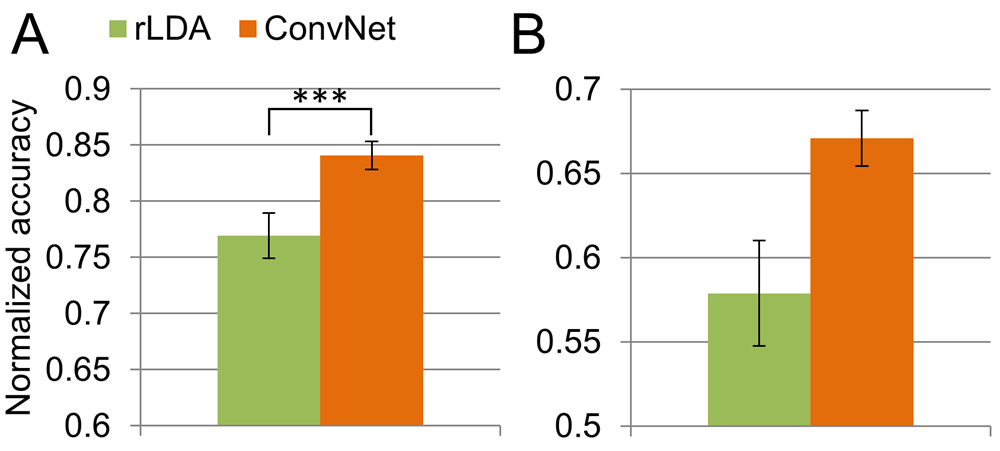
\includegraphics[width=.45\linewidth]{images/within-subject-flanker-gui.png}} \quad
    \subfloat[\textbf{Mean normalized decoding accuracy on unknown subjects.} Error bars show the SEM. A) Eriksen flanker task, trained on 30 subjects, tested on 1 subject.  Deep ConvNets were 5.05\% better than rLDA, p = 3.16 *10-4 (paired t-test). B) Online GUI control. Trained on 3 subjects, tested on the  respective remaining subject. Figure from \citet{volker2018deep}.]
    {\label{cross-subject-flanker-gui-fig}
        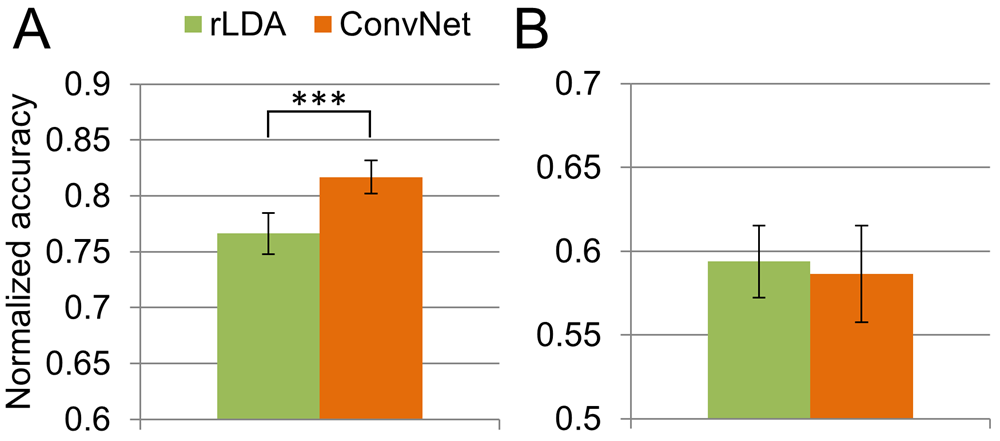
\includegraphics[width=.45\linewidth]{images/cross-subject-flanker-gui.png}} 
    \caption[Error decoding accuracy on Eriksen flanker task and online GUI control]{\textbf{Error decoding accuracy on Eriksen flanker task and online GUI control.}}
\end{figure}


    In two additional error-related decoding experiments, we evaluated an
Eriksen flanker task and errors during an the online control of a
graphical user interface through a brain-computer-interface. In the
Eriksen flanker task, the subjects were asked to press the left or right
button on a gamepad depending on whether an `L' or an `R' was the middle
character of a 5-letter string displayed on the screen. For the online
graphical user interface (GUI) control, the subjects were given an aim
to reach using the GUI, also see \Cref{online-bci}. They had to
think of one of the classes of the aforementioned Mixed Imagery Dataset
to choose one of four possible GUI actions. The correct GUI action was
always determined by the specificed aim given to the subject, hence an
erroneous action could be detected. The decoding task in this paper was
to distinguish whether the BCI-selected action was correct or erroneous.
Results in \Cref{within-subject-flanker-gui-fig} and
\Cref{cross-subject-flanker-gui-fig} show that deep ConvNets
outperform rLDA in all settings except cross-subject error-decoding for
online GUI control, where the low number of subjects (4) may prevent the
ConvNets to learn enough to outperform rLDA.

\section{Proof-of-Concept Assistive
System}\label{online-bci}


\begin{figure}[htb]
    \myfloatalign
    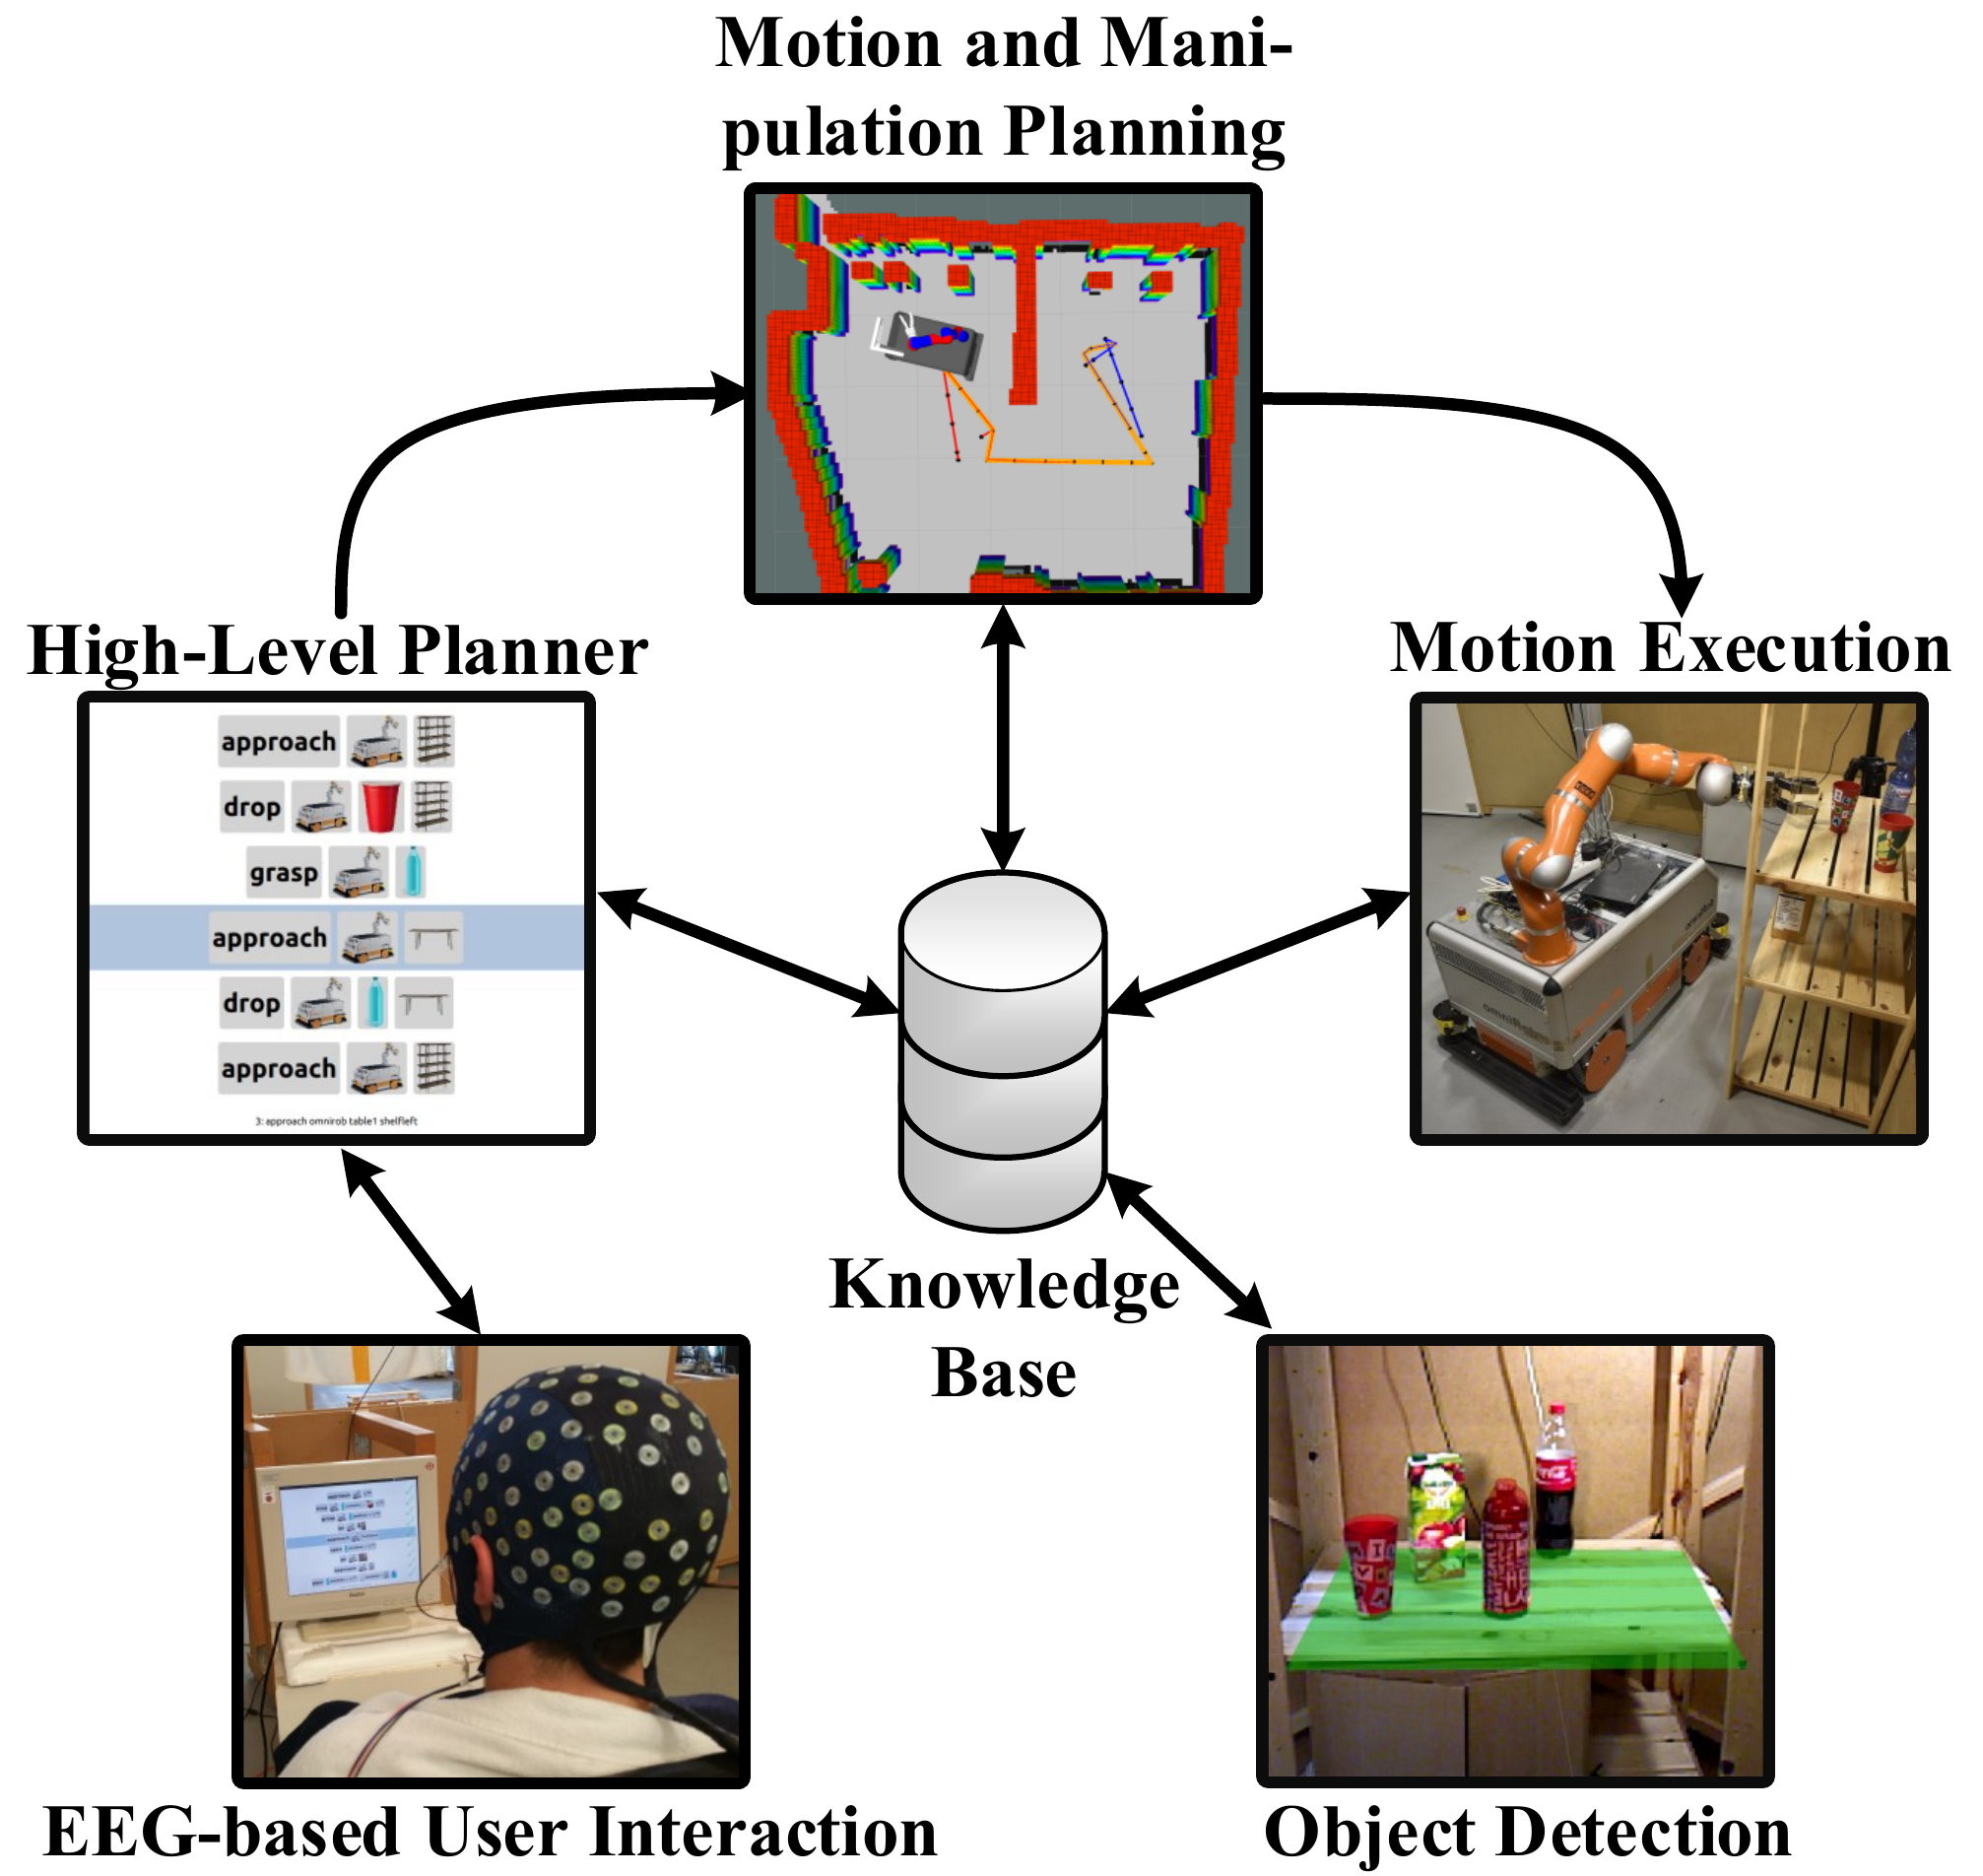
\includegraphics[width=0.5\linewidth]{images/robot-bci-overview.png}
    \caption[Overview of the proof-of-concept assistive system]{
\textbf{Overview of the proof-of-concept assistive system. The system
uses the deep ConvNet in the BCI component.} Robotic arm could be given high-level commands via the BCI, high-level commands were extracted from a knowledge base. The commands were then autonomously planned and executed by the robotic arm. Figure
from \citet{burget2017acting}
}
\label{robot-bci-overview-fig}
\end{figure}



\begin{table}[htb]
    \myfloatalign
    \footnotesize
    \begin{tabularx}{\textwidth}{p{0.1\textwidth}p{0.1\textwidth}p{0.1\textwidth}p{0.1\textwidth}p{0.1\textwidth}p{0.1\textwidth}p{0.1\textwidth}}
    \toprule
        \tableheadlinewithwidth{0.11\textwidth}{Subject} &
        \tableheadlinewithwidth{0.11\textwidth}{Runs} &
        \tableheadlinewithwidth{0.11\textwidth}{Accu-racy [\%] } &
        \tableheadlinewithwidth{0.11\textwidth}{Time {[}s{]}} &
        \tableheadlinewithwidth{0.11\textwidth}{Steps} &
        \tableheadlinewithwidth{0.11\textwidth}{Path Optimality {[}\%{]}} &
        \tableheadlinewithwidth{0.11\textwidth}{Time / Step {[}s{]}} \\ 
        \midrule
S1 & 18 & 84.1 ± 6.1 & 125 ± 84 & 13.0 ± 7.8 & 70.1 ± 22.3 & 9 ± 2 \\
S2 & 14 & 76.8 ± 14.1 & 150 ± 32 & 10.1 ± 2.8 & 91.3 ± 12.0 & 9 ± 3 \\
S3 & 17 & 82.0 ± 7.4 & 200 ± 159 & 17.6 ± 11.4 & 65.7 ± 28.9 & 11 ± 4 \\
S4 & 3 & 63.8 ± 15.6 & 176 ± 102 & 26.3 ± 11.2 & 34.5 ± 1.2 & 6 ± 2 \\
Average & 13 & 76.7 ± 9.1 & 148 ± 50 & 16.7 ± 7.1 & 65.4 ± 23.4 & 9 ±
2 \\
        \bottomrule
    \end{tabularx}
    \caption[Decoding problems in deep-learning EEG decoding studies prior to our work.]{
    \textbf{Results for BCI control of the GUI.} Accuracy is
fraction of correct commands, time is time per command, steps is steps
needed to reach the aim, path optimality is ratio of miniminally needed
nubmer of steps to actually used number of steps when every step is
optimal, and time/step is time per step. Results from 
\citet{burget2017acting}.
    }  \label{bci-robot-results}
\end{table}



    We also evaluated the use of our deep ConvNet as part of an assistive
robot system where the brain-computer interface was sending high-level
commands to a robotic arm. In this proof-of-concept system, the robotic
arm could be instructed by the user via the BCI to fetch a cup and
directly move the cup to the persons mouth to drink from it. An overview
can be seen in \Cref{robot-bci-overview-fig}. Results from
\Cref{bci-robot-results} show that 3 out of 4 subjects had a
command accuracy of more than 75\% and were able to reach the target
using less than twice the steps of the minimal path through the GUI
(path optimality \textgreater{} 50\%).

\section{Intracranial EEG Decoding}\label{intracranial-eeg-decoding}

\subsection{Intracranial EEG Decoding of Eriksen Flanker
Task}\label{intracranial-eeg-decoding-of-eriksen-flanker-task}


\begin{table}[htb]
    \myfloatalign
    \footnotesize
    \begin{tabularx}{\textwidth}{p{0.2\textwidth}p{0.2\textwidth}p{0.2\textwidth}p{0.2\textwidth}}
    \toprule
        \tableheadlinewithwidth{0.2\textwidth}{Classifier} &
        \tableheadlinewithwidth{0.2\textwidth}{Balanced Accuracy} &
        \tableheadlinewithwidth{0.2\textwidth}{Accuracy Correct Class } &
        \tableheadlinewithwidth{0.2\textwidth}{Accuracy Error Class} \\ 
        \midrule
Deep4Net & 59.28 ± 0.50 & 69.37 ± 0.44 & 49.19 ± 0.56 \\
ShallowNet & 58.42 ± 0.32 & 74.83 ± 0.25 & 42.01 ± 0.40 \\
EEGNet & 57.73 ± 0.52 & 57.78 ± 0.48 & 57.68 ± 0.56 \\
rLDA & 53.76 ± 0.32 & 76.12 ± 0.26 & 31.40 ± 0.38 \\
ResNet & 52.45 ± 0.21 & 95.47 ± 0.14 & 09.43 ± 0.28 \\
        \bottomrule
    \end{tabularx}
    \caption[Decoding problems in deep-learning EEG decoding studies prior to our work.]{
    \textbf{Results for single-channel intracranial decoding of
errors during an Eriksen flanker task.} Balanced Accuracy is the mean of
the accuracies for correct class ground truth labels and error class
ground truth labels. Results from 
\citet{volker2018intracranial}.
    }  \label{intracranial-error-results-table}
\end{table}
 

\begin{figure}[h!tb]
    \myfloatalign
    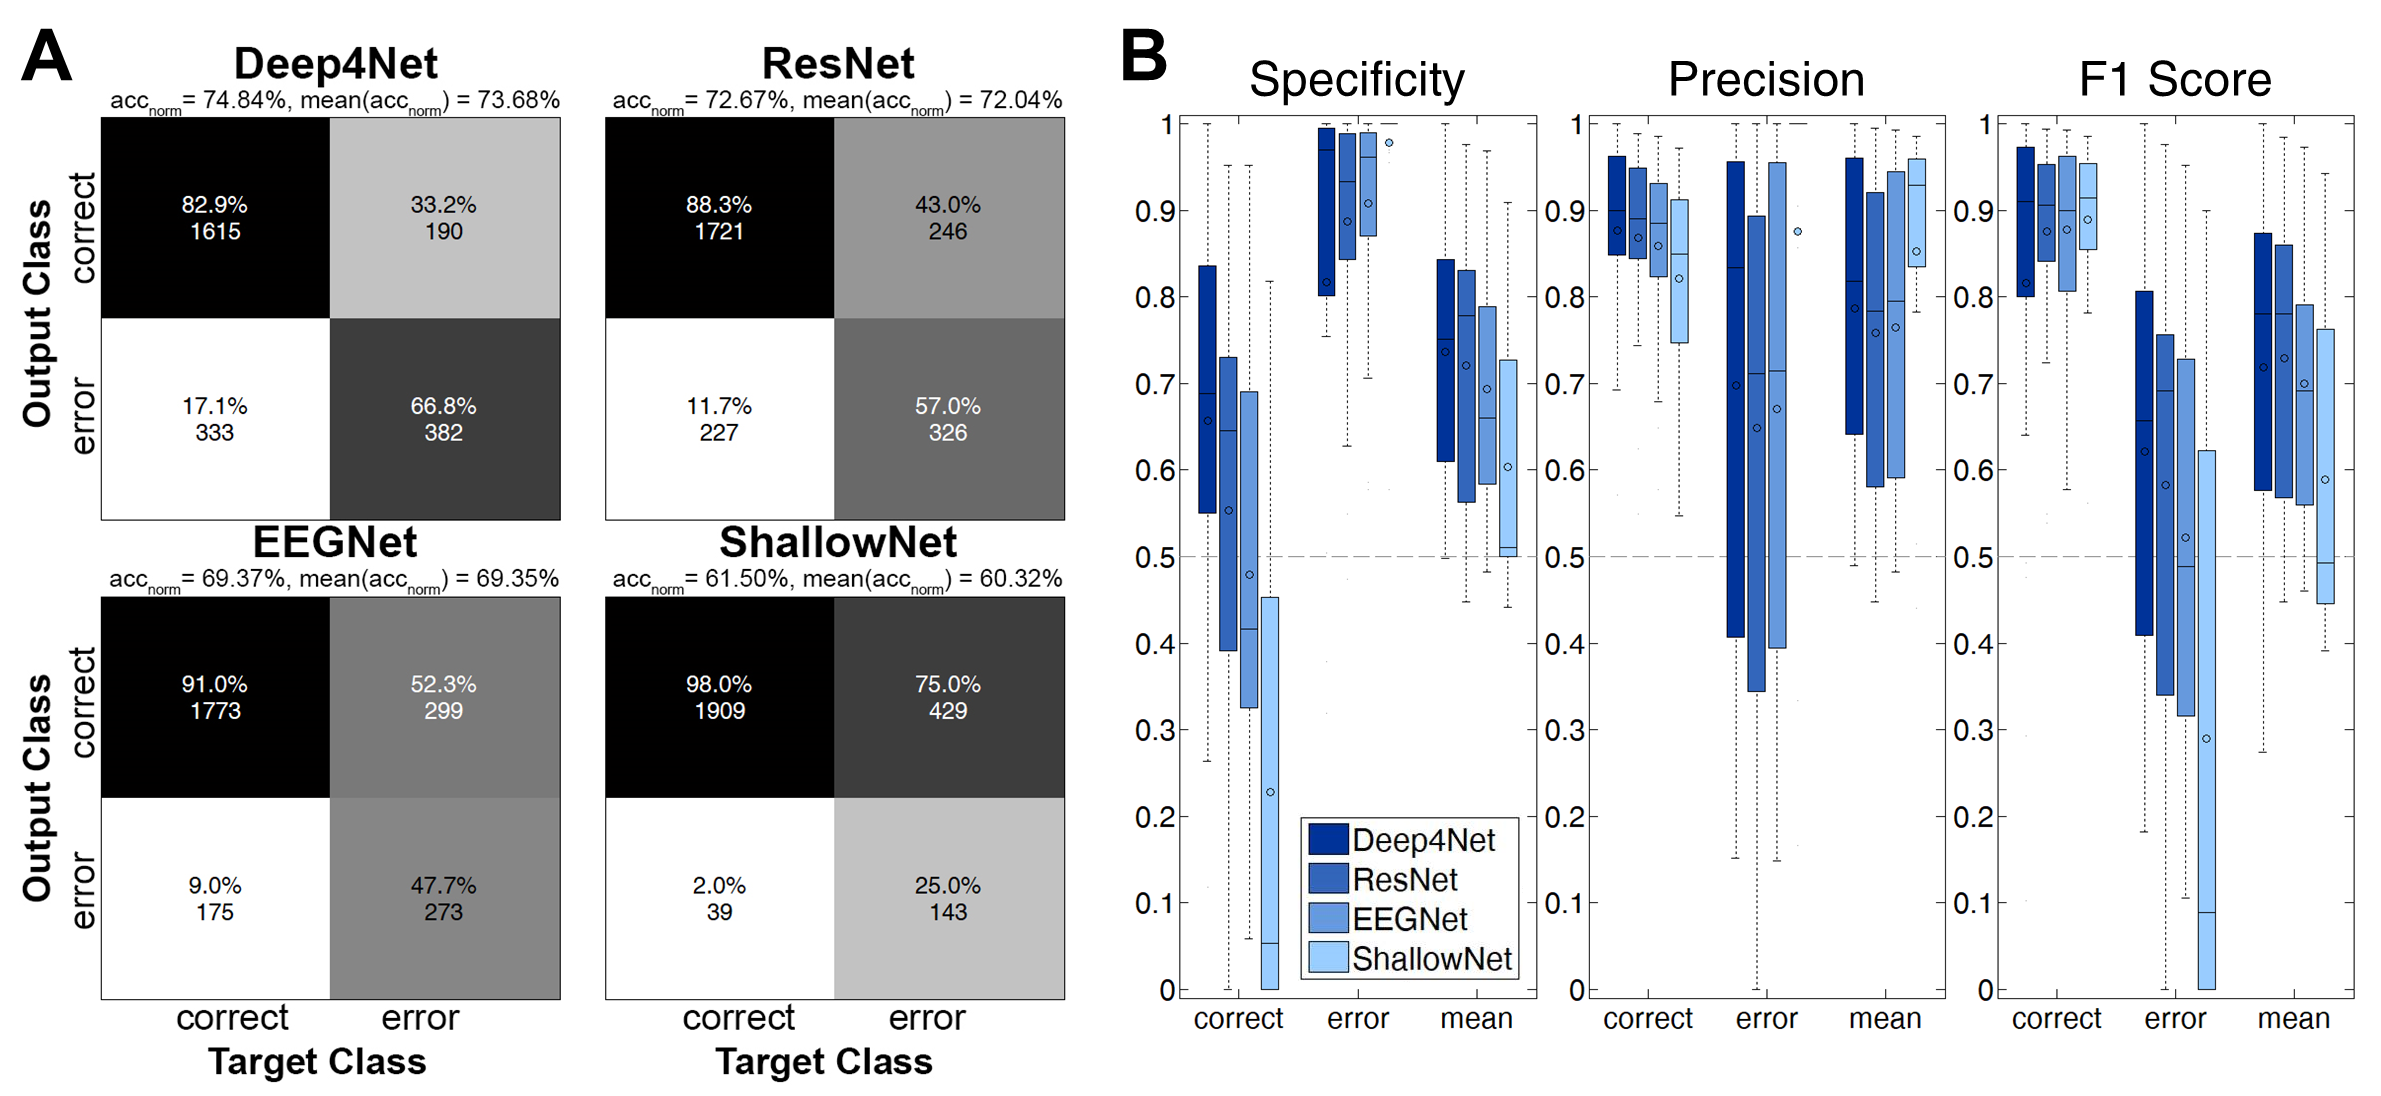
\includegraphics[width=1\linewidth]{images/IntracranialError.png}
    \caption[Results for all-channel intracranial decoding of errors during
an Eriksen flanker task]{
\textbf{Results for all-channel intracranial decoding of errors during
an Eriksen flanker task.} Here, the classifiers were trained on all
available channels per patient. A) Confusion matrices of the four models
used for decoding. The matrices display the sum of all trials over the
24 recordings. On top of the matrices, the class-normalized accuracy
(average over per-class accuracies) over all trials, i.e.,
$\mathrm{acc}_\mathrm{norm}$, and the mean of the single recordings'
normalized accuracy, i.e., $\mathrm{mean}(\mathrm{acc}_\mathrm{norm})$
is displayed; please note that these two measures differ slightly, as
the patients had a varying number of total trials and trials per class.
B) Box plots for specificity, precision and F1 score. The box represents
the interquartile range (IQR) of the data, the circle within the mean,
the horizontal line depicts the median. The lower whiskers include all
data points that have the minimal value of
$25^\mathrm{th} \mathrm{percentile}-1.5 \cdot \mathrm{IQR}$, the upper
whiskers include all points that are maximally
$75^\mathrm{th} \mathrm{percentile}+1.5 \cdot \mathrm{IQR}$. Figure
from \citet{volker2018intracranial}.
}
\label{intracranial-error-results-fig}
\end{figure}

    We further evaluated whether the same networks developed for noninvasive
EEG decoding can successfully learn to decode intracranial EEG.
Therefore, in one work we used the same Eriksen flanker task as
described in \Cref{flanker-and-gui-section}, but recorded
intracranial EEG from 23 patients who had pharmacoresistant epilepsy
\cite{volker2018intracranial}. Results for single-channel
decoding \Cref{intracranial-error-results-table} show the
deep and shallow ConvNet to clearly outperform rLDA (59.3\%/58.4\%
vs.~53.8\%) , whereas the residual ConvNet has low accuracy (52.5\%). In
contrast, results for all-channel decoding
\Cref{intracranial-error-results-fig} show the residual
ConvNet to perform well with the residual ConvNet and the deep ConvNet
outperforming the shallow ConvNet (72.1\% and 73.7\% vs.~60.3\%
class-normalized accuracies (average over per-class accuracies)).

\subsection{Transfer Learning for Intracranial Error
Decoding}\label{transfer-learning-for-intracranial-error-decoding}

\begin{figure}[h!tb]
    \myfloatalign
    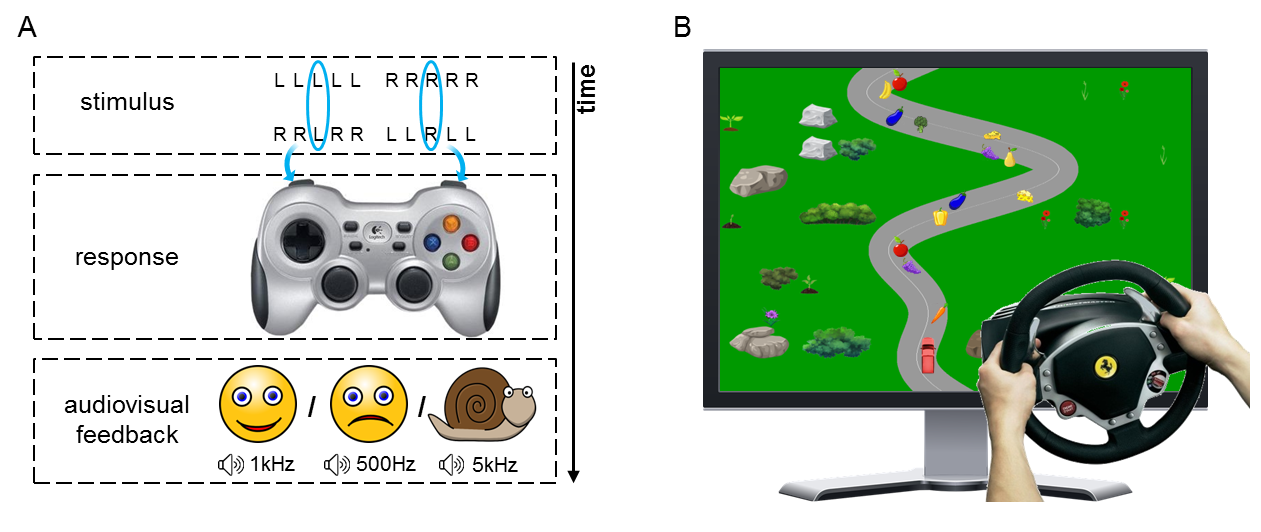
\includegraphics[width=0.7\linewidth]{images/eriksen-flanker-car-driving-tasks.png}
    \caption[Visualizations of Eriksen flanker and  car driving task]{
\textbf{Sketch of the Eriksen flanker task (A) and screenshot of the car
driving task (B).} Figure from \citet{behncke2018cross}. 
}
\label{eriksen-flanker-car-driving-tasks-fig}
\end{figure}


\begin{figure}[h!tb]
    \myfloatalign
    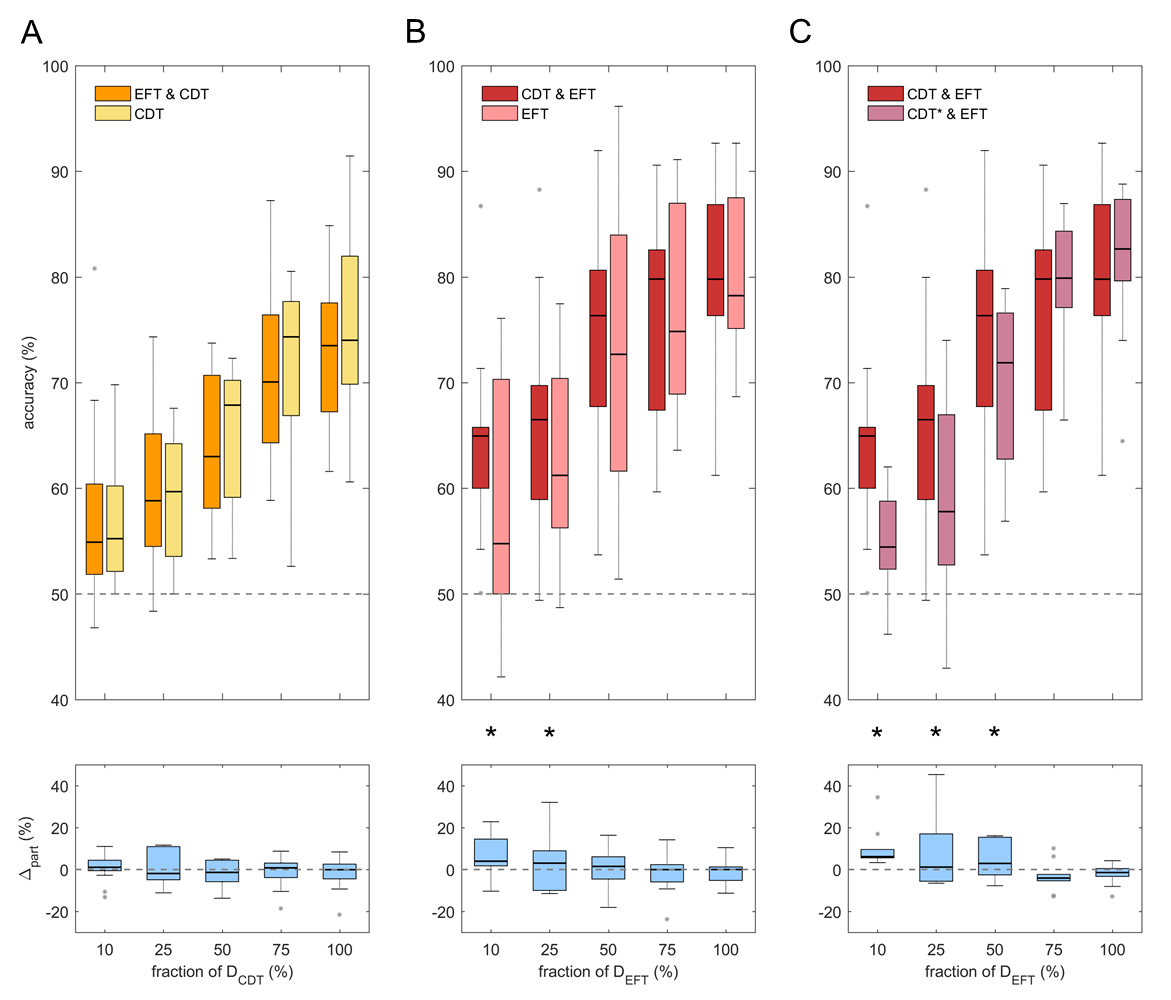
\includegraphics[width=0.8\linewidth]{images/cross-training-eft-cdt-results.png}
    \caption[Results for transfer learning on the Eriksen flanker task and the car driving task]{
\textbf{Results for transfer learning on the Eriksen flanker task (EFT)
and the car driving task (CDT).} All results are computed for a varying
fraction of available data for the target decoding task (bottom row).
\textbf{A} compares CDT accuracies after training only on CDT or
pretraining on EFT and finetuning on CDT. \textbf{B} compares EFT
accuracies after only training on EFT or after pretraining on CDT and
finetuning on EFT. As a sanity check for the results in \textbf{B},
\textbf{C} compares EFT accuracies when pretraining on original CDT data
and finetuning on EFT to pretraining on CDT data with shuffled labels
(CDT*) and finetuning on EFT. Results show that pretraining on CDT helps
EFT decoding when little EFT data is available. Figure from
\citet{behncke2018cross}.
}
\label{cross-training-eft-cdt-results-fig}
\end{figure}


    We further tested the potential of ConvNets to transfer knowledge
learned from decoding intracranial signals in error-decoding paradigm to
decoding signals in another a different error-decoding paradigm
\cite{behncke2018cross}. The two error-decoding paradigms were
the aforementioned Eriksen flanker task (EFT) and a car driving task
(CDT), where subjects had to use a steering wheel to steer a car in a
computer game and avoid hitting obstacles, where hitting an obstacle was
considered an error event (see
\Cref{eriksen-flanker-car-driving-tasks-fig}). Results in
\Cref{cross-training-eft-cdt-results-fig} show that
pretraining on CDT helps EFT decoding when few EDT data is available.

\subsection{Microelectrocorticography Decoding of Auditory Evoked
Responses in
Sheep}\label{microelectrocorticography-decoding-of-auditory-evoked-responses-in-sheep}



\begin{figure}[bth]
    \myfloatalign
    \subfloat[\textbf{Decoding tasks overview.}]
    {\label{sheep-sounds-fig}
    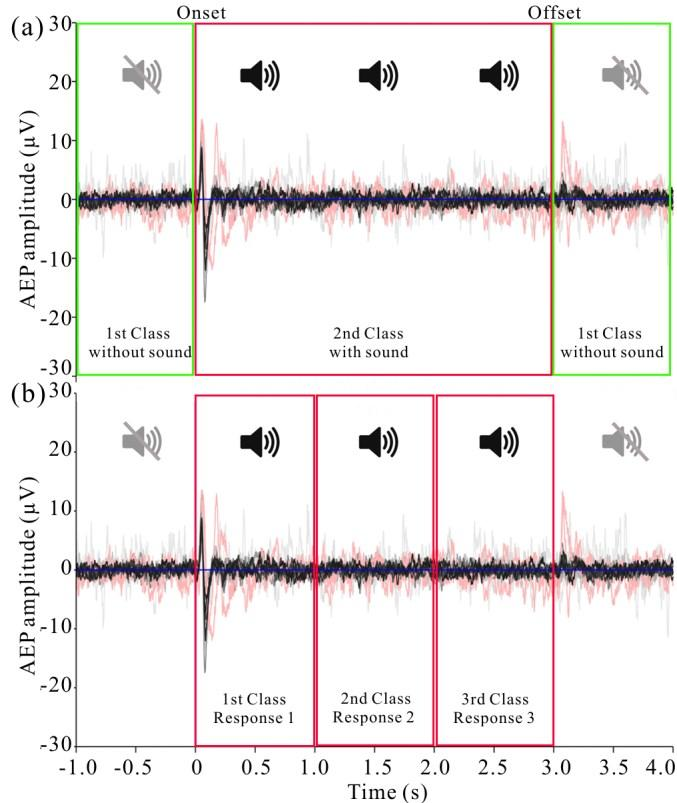
\includegraphics[width=.39\linewidth]{images/sheep-sounds.jpg}} \quad
    \subfloat[\textbf{Results.}]
    {\label{sheep-accuracies-fig}
        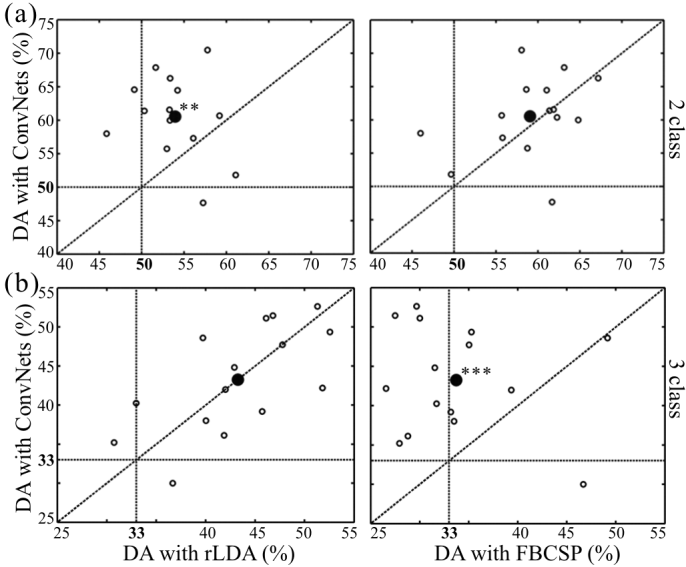
\includegraphics[width=.56\linewidth]{images/sheep-accuracies.png}} 
    \caption[Auditory evoked responses in sheep]{
    \textbf{Overview over tasks and results of decoding auditory evoked responses in sheep.} Left: Overview over decoding tasks. First task (top) was to
distingish 3 seconds when the sound was playing from the second before
and the second after. Second task (bottom) was to distinguish the first,
second and third second during theplaying of the sound. Signals are
averaged responses from one electrode during different days, with black
and grey being signals while the sheep was awake and red ones while the
sheep was under general anesthesia.  Right: Results of decoding auditory evoked responses from sheep.
rlDA, FBSCP and the deep ConvNet were the decoding models. Open circles represent accuracies for individual experiment days and closed circles represent the average
over these accuracies. 

Figures from \citet{wangsheep}.}
    \label{sheep-fig}
\end{figure}



    In this study, we evaluated the ConvNets for decoding auditory evoked
responses played to a sheep that was chronically implanted with a 

$\mu$ECoG-based neural interfacing device \cite{wangsheep}.

3-seconds-long sounds were presented to the sheep and two decoding tasks
were defined from those 3 seconds as well as the second immediately
before and after the playing of the sound. The first decoding task was
to distinguish the 3 seconds when the sound was playing from the second
immediately before and the second immediately after the sound. The
second task was distinguishing the first, second and third second of the
playing of the sound to discriminate early, intermediate and late
auditory evoked response (see \Cref{sheep-sounds-fig}).
Results in \Cref{sheep-accuracies-fig} show that the deep
ConvNet can perform as good as FBSCP and rLDA, and perform well on both
tasks, whereas rLDA performs competitively only on the first and FBSCP
only on the second task.

\section{Evaluation on Large-Scale Task-Diverse
Dataset}\label{evaluation-on-large-scale-task-diverse-dataset}


\begin{table}[htb]
    \myfloatalign
    \footnotesize
    \begin{tabularx}{\textwidth}{p{0.2\textwidth}p{0.1\textwidth}p{0.2\textwidth}p{0.1\textwidth}p{0.1\textwidth}p{0.1\textwidth}}
    \toprule
        \tableheadlinewithwidth{0.2\textwidth}{Name (Acronym)} &
        \tableheadlinewithwidth{0.1\textwidth}{\#Classes} &
        \tableheadlinewithwidth{0.2\textwidth}{Task type} &
        \tableheadlinewithwidth{0.1\textwidth}{\#Sub-jects}&
        \tableheadlinewithwidth{0.1\textwidth}{Trials per subject}&
        \tableheadlinewithwidth{0.1\textwidth}{Class balance} \\ 
        \midrule
High-Gamma Dataset (Motor) & 4 & Motor task & 20 & 1000 & balanced \\
KUKA Pouring Observation (KPO) & 2 & Error observation & 5 & 720-800 &
balanced \\
Robot-Grasping Observation (RGO) & 2 & Error observation & 12 & 720-800
& balanced \\
Error-Related Negativity (ERN) & 2 & Eriksen flanker task & 31 & 1000 &
1/2 up to 1/15 \\
Semantic Categories & 3 & Speech imagery & 16 & 750 & balanced \\
Real vs.~Pseudo Words & 2 & Speech imagery & 16 & 1000 & 3/1 \\
        \bottomrule
    \end{tabularx}
    \caption[Datasets for the large-scale evaluation framework]{
    \textbf{Datasets for the large-scale evaluation framework.} Used in \citet{heilmeyer2018large}.
    }  \label{large-framework-overview-table}
\end{table}


\begin{figure}[htb]
    \myfloatalign
    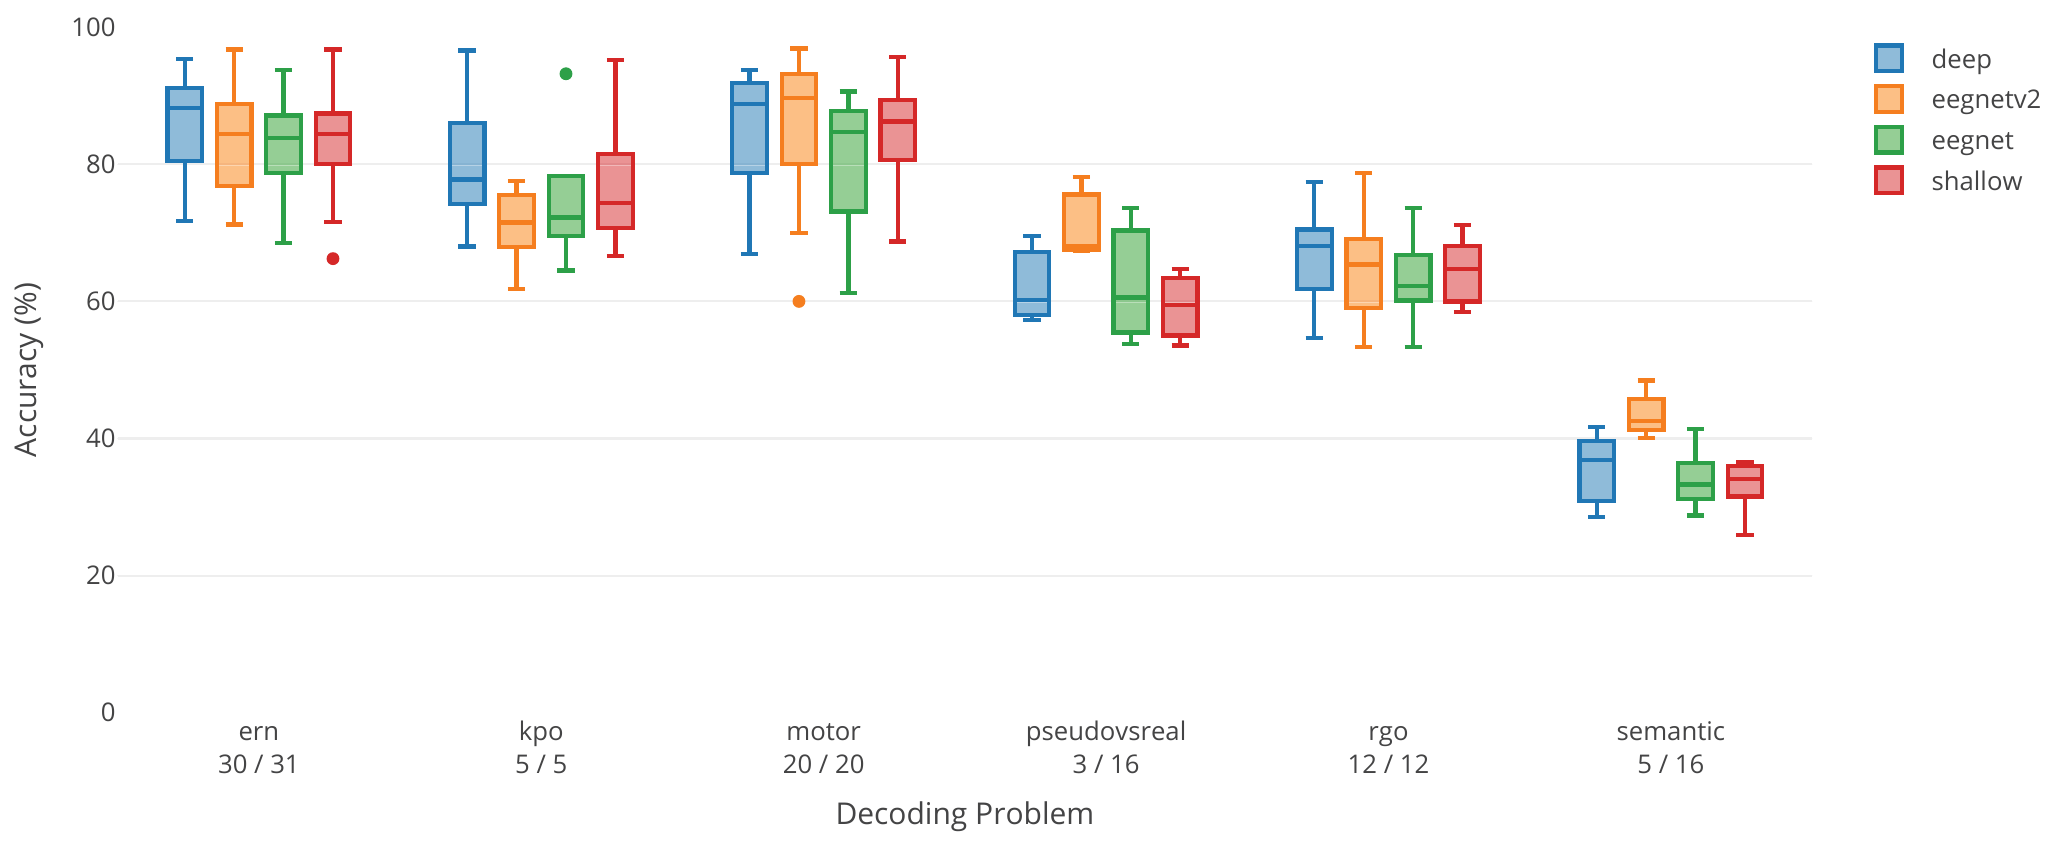
\includegraphics[width=1\linewidth]{images/large-framework-per-dataset-results.png}
    \caption[Large-scale evaluation results]{
\textbf{Per-dataset results for the large-scale evaluation of deep
ConvNet, shallow ConvNet and two versions of EEGNet.} Boxplots show the
distribution over per-subject accuracies for the individual decoding
tasks. ern, kpo and rgo are the error-related datasets, ern:
Error-related negativity Eriksen flanker task, KPO: KUKA Pouring
Observation paradigm, rgo: robot-grasping observation paradigm. motor is
the high-gamma dataset with 6 additional subjects that were excluded for
data quality reasons from \cite{schirrmeisterdeephbm2017}.
pseudovsreal and semantic are two semantic processing datasets to
classify silent repetitions of pseudowords vs.~realwords (pseudovsreal)
or different semantic categories (semantic) . Figure from
\citet{heilmeyer2018large}.
}
\label{large-framework-per-dataset-results-fig}
\end{figure}


\begin{figure}[htb]
    \myfloatalign
    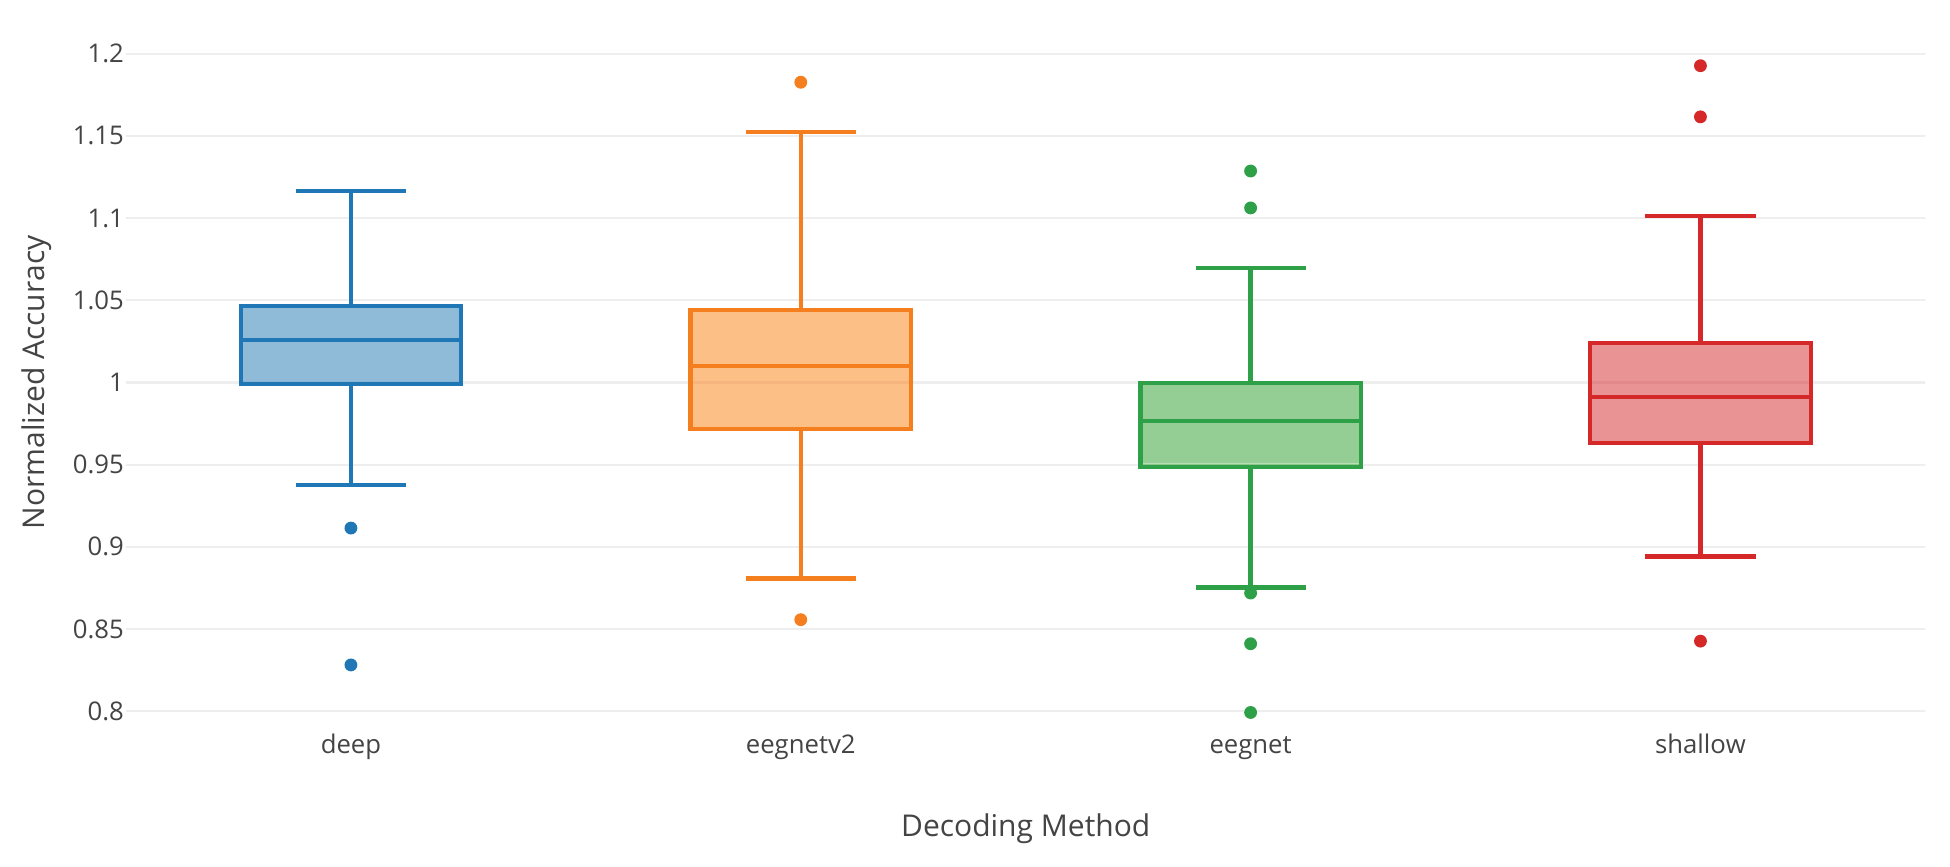
\includegraphics[width=1\linewidth]{images/large-framework-averaged-results.png}
    \caption[Large-scale dataset-averaged evaluation results]{
\textbf{Dataset-averaged results for the large-scale evaluation of deep
ConvNet, shallow ConvNet and two versions of EEGNet.} Accuracies are
normalized to the average of the accuracies of all models. Figure from
\citet{heilmeyer2018large}.
}
\label{large-framework-averaged-results-fig}
\end{figure}


\begin{table}[htb]
    \myfloatalign
    \footnotesize
    \begin{tabularx}{\textwidth}{p{0.3\textwidth}p{0.3\textwidth}p{0.3\textwidth}}
    \toprule
        \tableheadlinewithwidth{0.3\textwidth}{Network} &
        \tableheadlinewithwidth{0.3\textwidth}{Mean accuracy} &
        \tableheadlinewithwidth{0.3\textwidth}{Mean normalized accuracy} \\ 
        \midrule
Deep ConvNet & 70.08\% ± 20.92\% & 1.00 ± 0.05 \\
EEGNetv2 & 70.00\% ±18.86\% & 1.02 ± 0.08 \\
EEGNet & 67.71\% ± 19.04\% & 0.98 ± 0.06 \\
Shallow ConvNet & 67.71\% ±19.04\% & 0.99 ± 0.06 \\
        \bottomrule
    \end{tabularx}
    \caption[Datasets for the large-scale evaluation framework]{
    \textbf{Dataset-averaged results for the large-scale
evaluation of deep ConvNet, shallow ConvNet and two versions of EEGNet.}
Accuracies are normalized to the average of the accuracies of all
models. Results from \citet{heilmeyer2018large}.
    }  \label{large-framework-results-table}
\end{table}




We also compared the deep and shallow ConvNet architectures as well as
EEGNet on six classification tasks with more than 90000 trials in total
(see \Cref{large-framework-overview-table})
\citep{heilmeyer2018large}. The datasets tasks were all
recorded in our lab and included the high-gamma dataset, three
error-related tasks described before (Eriksen flanker task, robot
grasping and robot pouring observations) as well as two tasks on
semantic processing. In the semantic processing dataset, the
classification tasks were to distinguish different types of words that a
subject silently repeated \cite{Rau:2015uk}. The first task
was to distinguish existing real words from nonexisting pseudowords. The
second classification task was to distingiush three semantic categories
(food, animals, tools) the word may belong to. The evaluation code for
all models always used the original code and hyperparameters from the
original studies in order to ensure a fair comparison. Results show that
the deep ConvNet and the more recent version of EEGNet (EEGNetv2)
perform similarly well, with shallow and an older version of EEGNet
performing slightly worse, see
\Cref{large-framework-per-dataset-results-fig},
\Cref{large-framework-averaged-results-fig} and
\Cref{large-framework-results-table}.

\begin{openbox}
\item How do these networks perform on non-trial-based tasks like pathology decoding?
\end{openbox}

%************************************************
\chapter{Decoding Pathology}\label{pathology}
%**************************************

\begin{startbox}{ConvNets diagnose pathology with good accuracy even from very short amounts of time} 
\item ConvNets reach around 85% accuracy
\item Can reach high accuracies using a single minute per recording during inference
\item Struggle with recordings where contextual features like age and sleep affect the doctors diagnosis
\item Seem to learn temporal slowing indicates pathology, strong occipital alpha indicates healthy
\end{startbox}


    We also evaluated our deep ConvNets for automatic medical diagnosis from
EEG. EEG is important in clinical practice both as a screening method as
well as for hypothesis-based diagnostics, e.g., in epilepsy or stroke.
One of the main limitations of using EEG for diagnostics is the required
time and specialized knowledge of experts that need to be well-trained
on EEG diagnostics to reach reliable results. Therefore, a deep-learning
approach that aids in the diagnostic process could make EEG diagnosis
more widely accessible, reduce time and effort for clinicians and
potentially make diagnoses more accurate. 

Text and figures in this
section are adapted from \citet{schirrmeisterdeeppathology}.
I was the main contributor to
\citet{schirrmeisterdeeppathology}.

\section{Dataset and Preprocessing}\label{dataset-and-preprocessing}

\subsection{Temple University Hospital EEG Abnormal
Corpus}\label{temple-university-hospital-eeg-abnormal-corpus}

\begin{table}[htb]
    \myfloatalign
    \begin{tabularx}{\textwidth}{p{0.15\textwidth}p{0.3\textwidth}p{0.2\textwidth}p{0.2\textwidth}}
    \toprule
        &
        &
        \tableheadlinewithwidth{0.2\textwidth}{Files} &
        \tableheadlinewithwidth{0.2\textwidth}{Patients} \\ 
        \midrule
    
        Train & Normal & 1379 (50\%) & 1238 (58\%) \\
        & Pathological & 1361(50\%) & 894 (42\%) \\
        & Rater Agreement & 2704 (99\%) & 2107 (97\%) \\
        & Rater Disagreement & 36 (1\%) & 25 (0\%) \\
        Evaluation & Normal & 150 (54\%) & 148 (58\%) \\
        & Pathological & 127 (46\%) & 105 (42\%) \\
        & Rater Agreement & 277 (100\%) & 253 (100\%) \\
        & Rater Disagreement & 0 (0\%) & 0 (0\%) \\
        \bottomrule
    \end{tabularx}
    \caption[TUH EEG Abnormal Corpus 1.1.2 Statistics]{
    \textbf{TUH EEG Abnormal Corpus 1.1.2 Statistics.} Obtained
from \url{https://www.isip.piconepress.com/projects/tuh_eeg/}. Rater
agreements refer to the agreement between the student annotator of the
file and the medical report written by a certified neurologist.
}
    \label{table-tuh-dataset}
\end{table}



    We used the Temple University Hospital (TUH) EEG Abnormal Corpus for
evaluating our deep ConvNets on pathology detection from EEG. The Temple
University Hospital (TUH) EEG Abnormal Corpus 1.1.2 is a dataset of
manually labeled normal and pathological clinical EEG recordings. It is
taken from the TUH EEG Data Corpus which contains over 16000 clinical
recordings of more than 10000 subjects from over 12 years
\citep{obeid\_temple\_2016}. The Abnormal Corpus contains
3017 recordings, 1529 of which were labeled normal and 1488 of which
were labeled pathological. The Corpus was split into a training and
evaluation set, see \Cref{table-tuh-dataset}. Recordings
were acquired from at least 21 standard electrode positions and with a
sampling rate of in most cases 250 Hz. Per recording, there are around
20 minutes of EEG data. The inter-rater agreement on between the medical
report of a certified neurologist and a medical student annotator was
99\% for the training recordings and 100\% for the evaluation
recordings, also see \Cref{table-tuh-dataset}.

\subsection{Preprocessing}\label{preprocessing}

    We minimally preprocessed the data with these steps: 1. Select a subset
of 21 electrodes present in all recordings. 2. Remove the first minute
of each recording as it contained stronger artifacts. 3. Use only up to
20 minutes of the remaining recording to speed up the computations. 4.
Clip the amplitude values to the range of $\pm800$ $\mu V$ to reduce
the effects of strong artifacts. 5. Resample the data to 100 Hz to
further speed up the computation.

\subsection{Decoding from Reduced EEG Time
Segments}\label{decoding-from-reduced-eeg-time-segments}

    We also evaluated the ConvNets on reduced versions of the datasets,
using only the first 1, 2, 4, 8, or 16 minutes after the first minute of
the recording (the first minute of the recordings was always excluded
because it appeared to be more prone to artifact contamination than the
later time windows). We reduced either only the training data, only the
test data, or both. These analyses were carried out to study how long
EEG recordings need to be for training and for predicting EEG
pathologies with good accuracies.

\section{Network Architectures}\label{network-architectures}

    We used our deep and shallow ConvNets with only minor modifications to
the architecture. To use larger time windows to make a single
prediction, we adapted the architectures by changing the final layer
kernel length so the ConvNets have an input length of about 600 input
samples, which correspond to 6 seconds for the 100 Hz EEG input.
Additionally, we moved the pooling strides of the deep ConvNet to the
convolutional layers directly before each pooling. This modification,
which we initially considered a mistake, allowed us to grow the ConvNet
input length without strongly increased computation times and provided
good accuracies in preliminary experiments on the training data;
therefore we decided to keep it.

\section{Network Training}\label{network-training}

    As in other studies, we optimized the ConvNet parameters using
stochastic gradient descent with the optimizer Adam
\cite{kingma\_adam:\_2014}. To make best use of the available
data, we trained the ConvNets on maximally overlapping time crops using
cropped training as described in \Cref{cropped-training}. Code
to reproduce the results of this study is available under
https://github.com/robintibor/auto-eeg-diagnosis-example.

\section{Automatic Architecture
Optimization}\label{automatic-architecture-optimization}

    We also carried out a preliminary study of automatic architecture
optimization to further improve our ConvNet architectures. To that end,
we used the automatic hyperparameter optimization algorithm SMAC
\citep{hutter\_sequential\_2011} to optimize architecture
hyperparameters of the deep and shallow ConvNets, such as filter
lengths, strides and types of nonlinearities. As the objective function
to optimize via SMAC, we used 10-fold cross-validation performance
obtained on the first 1500 recordings of the training data (using each
fold as an instance for SMAC to speed up the optimization). We set a
time limit of 3.5 hours for each configuration run on a single fold.
Runs that timed out or crashed (e.g., networks configurations that did
not fit in GPU memory) were scored with an accuracy of 0\%.

\section{Deep and Shallow ConvNets Reached State-of-the-Art
Results}\label{deep-and-shallow-convnets-reached-state-of-the-art-results}

\begin{table}[htb]
    \footnotesize
    \myfloatalign
    \begin{tabularx}{\textwidth}{p{0.2\textwidth}p{0.15\textwidth}p{0.15\textwidth}p{0.15\textwidth}p{0.15\textwidth}}
    \toprule
        &
        \tableheadlinewithwidth{0.15\textwidth}{Accuracy}&
        \tableheadlinewithwidth{0.15\textwidth}{Sensitivity} &
        \tableheadlinewithwidth{0.15\textwidth}{Specificity} &
        \tableheadlinewithwidth{0.15\textwidth}{Crop-accuracy} \\ 
        \midrule
    
Baseline \citep{abnormalLopez} & 78.8 & 75.4 & 81.9 & n.a. \\
Deep & 85.4 & 75.1 & 94.1 & 82.5 \\
Shallow & 84.5 & 77.3 & 90.5 & 81.7 \\
Linear & 51.4 & 20.9 & 77.3 & 50.2 \\
        \bottomrule
    \end{tabularx}
    \caption[TUH pathology decoding accuracies]{
\textbf{Decoding accuracies for discriminating normal and
pathological EEG with deep and shallow ConvNets.} For deep and shallow
ConvNets, mean over five independent runs with different random seeds.
Deep and shallow ConvNet outperformed the feature-based deep learning
baseline. Note that the baseline was evaluated on an older version of the corpus that has since been corrected to not contain the same patient in training and test recordings among other things. Results from \citet{schirrmeisterdeeppathology}.
}
\label{pathology-convnet-results}
\end{table}

    Both the deep and the shallow ConvNet outperformed the only results that
had been published on the TUH Abnormal EEG Corpus at the time (see
\Cref{pathology-convnet-results}). Both ConvNets were more
than 5\% better than the baseline method of a convolutional network that
included multiple fully connected layers at the end and took precomputed
EEG features of an entire recording as one input
\citep{abnormalLopez}.The ConvNets as applied here reduced
the error rate from about 21\% to about 15\%. We also tested a linear
classifier on the same 6-second inputs as our ConvNets. The linear
classifier did not reach accuracies substantially different from chance
(51.4\%).

    Interestingly, both of our ConvNet architectures already reached higher
accuracies than the baseline when evaluating single predictions from
6-second crops. The average per-crop accuracy of individual predictions
was only about 3\% lower than average per-recording accuracy (averaged
predictions of all crops in a recording). Furthermore, the individual
prediction accuracies were already about 3\% higher than the
per-recording accuracies of the baseline. This implies that predictions
with high accuracies can be made from just 6 seconds of EEG data.


\begin{figure}[htbp]
\myfloatalign
\subfloat[]{%
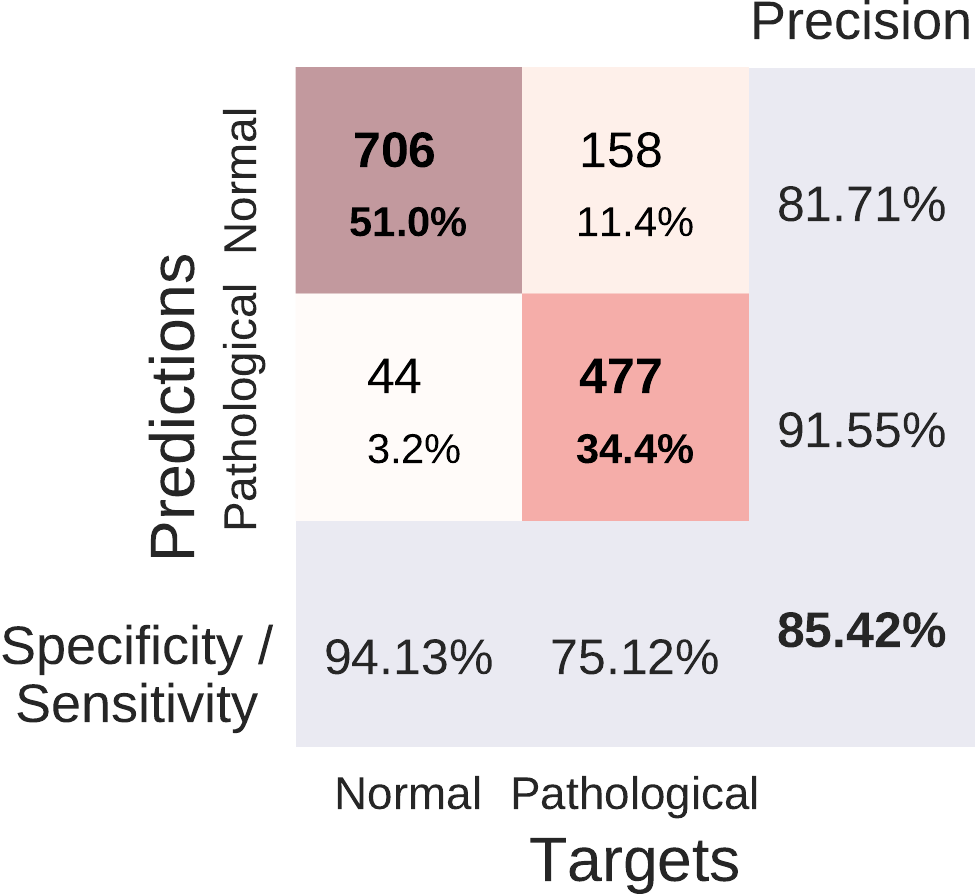
\includegraphics[width=0.408\linewidth]{images/ConfMatDeep.pdf-1.png}
}\hfill
\subfloat[]{%
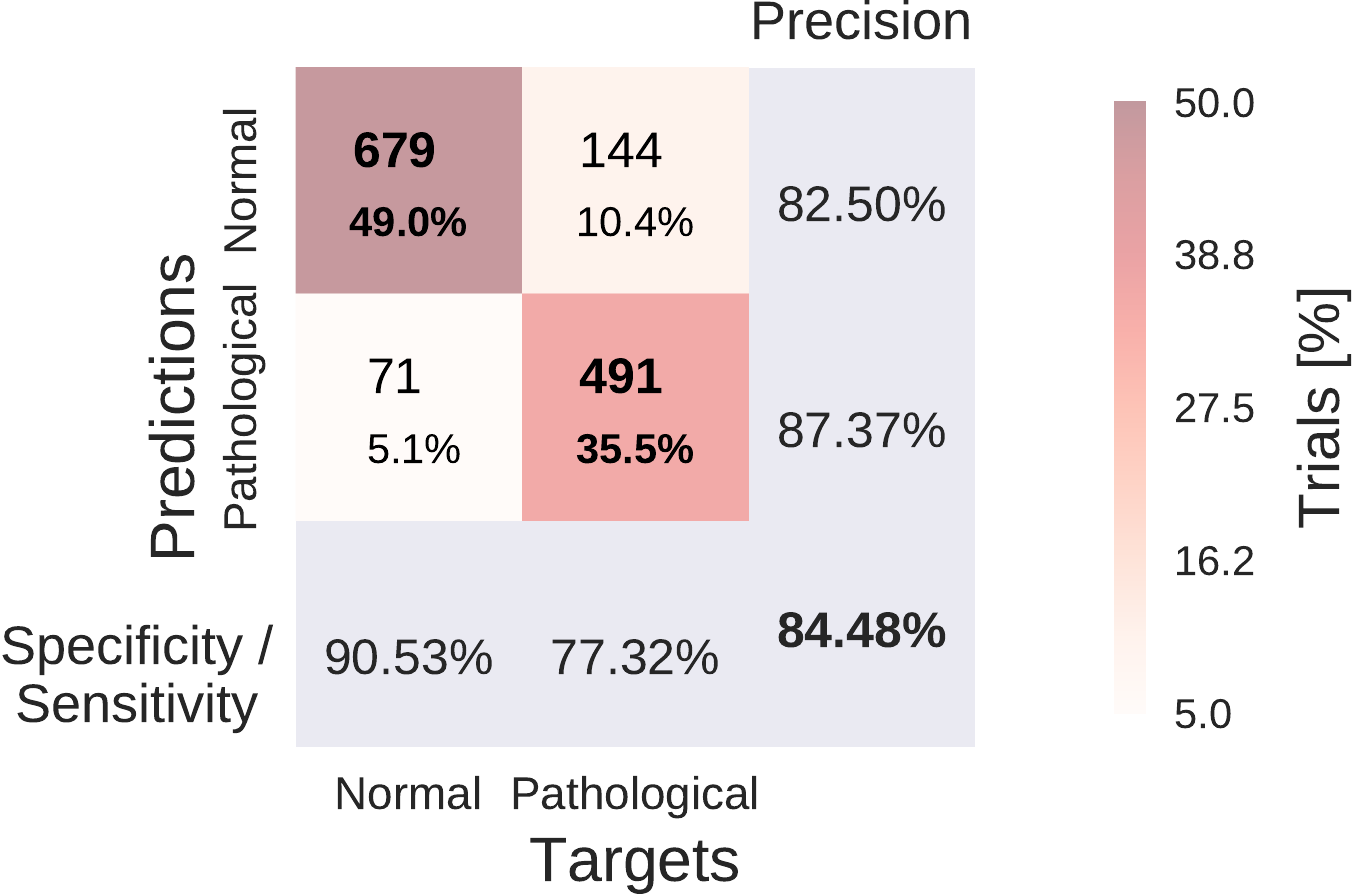
\includegraphics[width=0.562\linewidth]{images/ConfMatShallow.pdf-1.png}
}
\caption[Confusion Matrices for deep and shallow ConvNets]{\textbf{Confusion Matrices for deep and shallow ConvNets}, summed over five independent runs.
Each entry of row r and column c for upper-left 2x2-square: Number of trials of target r predicted as class c (also written in percent of all trials).
Bold diagonal corresponds to correctly predicted trials for both classes. Percentages and colors indicate fraction of trials in each cell relative to all trials.
The lower-right value: overall accuracy. The first two values in the bottom row correspond to sensitivity and specificity.
Rightmost column corresponds to precision defined as the number of trials correctly predicted for class r/number of trials predicted as class r. Figure from \citet{schirrmeisterdeeppathology}.}
\label{conf-mat-pathology-fig}
\end{figure}

    Both of our ConvNets made more errors on the pathological recordings, as
can be seen from \Cref{conf-mat-pathology-fig}. Both
ConvNets reached a specificity of above 90\% and a sensitivity of about
75-78\%. Confusion matrices between both approaches were very similar.
Relative to the baseline, they reached a similar sensitivity (0.3\%
smaller for the deep ConvNet, 1.9\% higher for the shallow ConvNet), and
a higher specificity (12.2\% higher for the deep ConvNet and 8.6\%
higher for the shallow ConvNet).

\begin{figure}[htbp]
\myfloatalign
\includegraphics[width=\linewidth]{images/Time_Plot.pdf-1.png}
\caption[Results on reduced datasets for deep ConvNet]{\textbf{Results on reduced datasets for deep ConvNet.} Train and/or test (evaluation) dataset was reduced from 20 minutes per recording to 1,2,4,8, or 16 minutes per recording, results are shown on the test set. Notably, when only reducing the duration of the test set recordings, maximal accuracies were observed  when using just 1 minute. We note that these results are each based on one run only; the slightly better performance than in \Cref{pathology-convnet-results} may thus be due to noise. Figure from \citet{schirrmeisterdeeppathology}.}
\label{pathology-time-fig}
\end{figure}

\begin{figure}[htbp]
\myfloatalign
\includegraphics[width=\linewidth]{images/Time_Crop_Pred_Plot.pdf-1.png}
\caption[Moving average of cropwise accuracies for the deep ConvNet.]{\textbf{Moving average of cropwise accuracies for the deep ConvNet.}
5-minute moving averages of the cropwise accuracies of the deep ConvNet, averaged over all test set recordings.
Dashed lines represent 5 individual training runs with different random seeds, solid black line represents mean over results for these runs.
x-axis shows center of 5-minute averaging window.
Figure from \citet{schirrmeisterdeeppathology}.}
\label{time-crop-pred-fig}
\end{figure}

    Deep ConvNets already reached their best trialwise accuracies with only
one minute of data used for the prediction. While the reduction of the
amount of length of the training data led to crop- and trialwise
accuracy decreases on the test data, reductions in the test data did not
have such an effect (see \Cref{pathology-time-fig}).
Remarkably, both crop- and trialwise accuracies slightly decreased when
going from 1 minute to 2 or 4 minutes of test data. To investigate
whether earlier parts of the recordings might be more informative, we
also computed a 5-minute moving average of the cropwise accuracies on
the test data for the Deep ConvNet trained on the full data. We show the
average over all recordings for these moving averages in (see
\Cref{time-crop-pred-fig}). Noticeably, as expected,
accuracies slightly decreased with increasing recording time. However,
the decrease is below 0.5\% and thus should be interpreted cautiously.

\section{Architecture Optimization Yielded Unexpected New
Models}\label{architecture-optimization-yielded-unexpected-new-models}


\begin{figure}[htbp]
\myfloatalign
\includegraphics[width=\linewidth]{images/ShallowSmacNet.pdf-1.png}
\caption[Final shallow ConvNet architecture selected by SMAC]{\textbf{Final shallow ConvNet architecture selected by SMAC.}
Conventions as in Fig. \ref{fig:shallow-convnet}.
Note that max pooling is the only nonlinearity SMAC decided to use. Figure from \citet{schirrmeisterdeeppathology}.}
\label{pathology-smac-results}
\end{figure}


\begin{table}[htb]
    \myfloatalign
    \begin{tabularx}{\textwidth}{p{0.15\textwidth}p{0.25\textwidth}p{0.1\textwidth}p{0.1\textwidth}p{0.1\textwidth}p{0.1\textwidth}}
    \toprule
        &
        \tableheadlinewithwidth{0.25\textwidth}{Architecture configuration} &
        \tableheadlinewithwidth{0.1\textwidth}{Trial} &
        \tableheadlinewithwidth{0.1\textwidth}{Crop} &
        \tableheadlinewithwidth{0.1\textwidth}{Trial} &
        \tableheadlinewithwidth{0.1\textwidth}{Crop} \\ 
        \midrule
\textbf{Deep} & Default & 84.2 & 81.6 & 85.4 & 82.5 \\
& Optimized & 86.3 & 80.9 & 84.5 & 81.3 \\
\textbf{Shallow} & Default & 84.5 & 82.1 & 84.5 & 81.7 \\
& Optimized & 85.9 & 80.3 & 83.0 & 79.8 \\
        \bottomrule
    \end{tabularx}
    \caption[SMAC pathology decoding results]{
    \textbf{Decoding accuracies with the default of deep and
shallow ConvNets as well as versions optimized by automatic architecture
optimization.} Train here refers to 10-fold cross-validation on the 1500
chronologically earliest recordings of the training data.
. Results from \citet{schirrmeisterdeeppathology}.
}  \label{pathology-smac-results}
\end{table}

    The models discovered by automated architecture optimization were
markedly different from our original deep and shallow ConvNets. For
example, the optimized architectures used only 1.8 and 3.7 seconds of
EEG data for the optimized deep and shallow ConvNet, respectively, in
contrast to about 6 seconds in the original versions. While the improved
performance of these modified architectures for the 10-fold
cross-validation on the training dataset (2.1\% and 1.4\% improvement
for deep and shallow ConvNets, respectively) did not generalize to the
evaluation set (0.9\% and 1.5\% deterioration for deep and shallow
ConvNets, respectively, see \Cref{pathology-smac-results}),
the modifications to the original network architectures already provided
interesting insights for further exploration: For example, in the case
of the shallow ConvNet, the modified architecture did not use any of the
original nonlinearities, but used max pooling as the only nonlinearity
(see Fig. \Cref{shallow-smac-net-fig}), a configuration we
had not considered in our manual search so far.

    \hypertarget{visualization}{%
\section{Visualization}\label{visualization}}

    We analyzed the spectral power changes in the data itself and the
spectral characteristics of the function the deep networks learned on
the data.

    To understand class-specific spectral characteristics in the EEG
recordings, we analyzed band powers in five frequency ranges: delta
(0--4 Hz), theta (4--8 Hz), alpha (8--14 Hz), low beta (14--20 Hz), high
beta (20--30 Hz) and low gamma (30--50 Hz).

For this, we performed the following steps: 1. Compute a short-term
Fourier transformation with window size 12 seconds and overlap 6 seconds
using a Blackman-Harris window. 2. Compute the median over all band
powers of all windows and recordings in each frequency bin;
independently for pathological and normal recordings. 3. Compute the log
ratio of these median band powers of the pathological and normal
recordings. 4. Compute the mean log ratio over all frequency bins in
each desired frequency range for each electrode. 5. Visualize the
resulting log ratios as a topographical map.

To better understand the spectral characteristics of the function the
ConvNets learned used in this study, we also used the perturbation-based
visualization method described in
\citet{schirrmeisterdeephbm2017}.

\begin{figure*}[htbp]
\centering
\subfloat[Pathological vs. normal relative spectral bandpower differences for the training set. Shown is the logarithm of the ratio of the median bandpower of the pathological  vs. normal (according to the experts' ratings) EEG recordings.]{%
\label{bandpower-pathology-fig}
\includegraphics[width=0.8\textwidth]{images/Bandpower.pdf-1.png}
}
\vspace{0.4cm}

\includegraphics[width=0.8\textwidth]{images/PerturbationDeep.pdf-1.png}
\hfill
\subfloat[Input-perturbation network-prediction correlation maps for the deep (top) and shallow (bottom) ConvNet. Correlation of predictions for the pathological class with amplitude perturbations. Scalp maps revealed for example a bilateral positive correlation for the delta and theta frequency ranges and a spatially more broadly distributed negative correlation for the beta and low gamma frequency ranges, indicating that the ConvNets used these frequency components in their decisions
]{
\label{perturbation-network-pathology-fig}
\includegraphics[width=0.8\textwidth]{images/PerturbationShallow.pdf-1.png}
}
\caption[Spectral power differences and input-perturbation network-prediction correlation maps]{\textbf{Spectral power differences and input-perturbation network-prediction correlation maps.} Figure from \citet{schirrmeisterdeeppathology}.}
\label{fig:visualization-results}
\end{figure*}

    Power was broadly increased for the the pathological class in the low
frequency bands (delta and theta range) and decreased in the beta and
low gamma ranges (\Cref{bandpower-pathology-fig}). Alpha
power was decreased for the occipital electrodes and increased for more
frontal electrodes.

    Scalp maps of the input-perturbation effects on predictions for the
pathological class for the different frequency bands showed effects
consistent with the power spectra in
(\Cref{perturbation-network-pathology-fig}). Both networks
strongly relied on the lower frequencies in the delta and theta
frequency range for their decoding decisions.

    \hypertarget{analysis-of-word-frequencies-in-the-medical-reports}{%
\section{Analysis of Word Frequencies in the Medical
Reports}\label{analysis-of-word-frequencies-in-the-medical-reports}}

    Furthermore, to better understand what kind of recordings are easier or
harder for the ConvNets to correctly decode, we analyzed the textual
clinical reports of each recording as included in the TUH Abnormal EEG
Corpus. Specifically, we investigated which words were relatively more
or less frequent in the incorrectly predicted recordings compared with
the correctly predicted recordings. We performed this analysis
independently for both the normal and the pathological class of
recordings. Concretely, for each class, we first computed the relative
frequencies $f_{i-}$ for each word $w_{i-}$ in the incorrectly
predicted recordings, i.e.:
$f_{i-} = \frac{|w_{i-}|}{\sum_{i}|w_{i-}|}$, where $|w_{i-}|$
denotes the number of occurrences for word $w_i$ in the incorrectly
predicted recordings. We then computed the frequencies $f_{i+}$ in the
same way and computed the ratios $r_i=f_{i-}/f_{i+}$. Finally, we
analyzed words with very large ratios ($\gg1$) and very small ratios
($\ll1$) by inspecting the contexts of their occurrences in the
clinical reports. This allowed us to gain insights into which
clinical/contextual aspects of the recordings correlated with ConvNets
failures.

Most notably, \texttt{small} and \texttt{amount} had a much larger word
frequency (15.5 times larger) in the incorrectly predicted pathological
recordings compared with the correctly predicted pathological
recordings. Closer inspection showed this is very sensible, as
\texttt{small\ amount} was often used to describe more subtle EEG
abnormalities (\texttt{small\ amount\ of\ temporal\ slowing},~
\texttt{Small\ amount\ of\ excess\ theta},~
\texttt{Small\ amount\ of\ background\ disorganization}, ~
\texttt{A\ small\ amount\ of\ rhythmic,} ~ \texttt{frontal\ slowing}), as this
subtlety of changes was likely the cause of the classification errors.

Secondly, other words with a notably different frequency were
\texttt{age} (9.7 times larger) and \texttt{sleep} (3 occurrences in 630
words of texts of incorrectly predicted recordings, not present in texts
of correctly predicted recordings). Both typically indicate the
clinician used the age of the subject or the fact that they were
(partially) asleep during the recording to interpret the EEG
(\texttt{Somewhat\ disorganized\ pattern\ for\ age},~
\texttt{Greater\ than\ anticipated\ disorganization\ for\ age.},~
\texttt{A\ single\ generalized\ discharge\ noted\ in\ stage\ II\ sleep.}).
Obviously, our ConvNets trained only on EEG do not have access to this
context information, leaving them at a disadvantage compared to the
clinicians and highlighting the potential of including contextual cues
such as age or vigilance in the training/decoding approach.

Inspection of the textual records of misclassified normal recordings did
not provide much insight, as they are typically very short (e.g.,
\texttt{Normal\ EEG.}, ~\texttt{Normal\ EEG\ in\ wakefulness.}).

Finally, consistent with the strong usage of the delta and theta
frequency range by the ConvNets as seen in the input-perturbation
network-prediction correlation maps
(\Cref{perturbation-network-pathology-fig}),
\texttt{slowing} and \texttt{temporal} are the 6th and 10th most
frequently occurring words in the textual reports of the pathological
recordings, while never occurring in the textual reports of the normal
recordings (irrespective of correct or incorrect predictions).

    \hypertarget{discussion}{%
\section{Discussion}\label{discussion}}

    To the best of our knowledge, the ConvNet architectures used in this
study achieved the best accuracies published so far on the TUH EEG
Abnormal Corpus. The architectures used were only very slightly modified
versions of ConvNet architectures that we previously introduced to
decode task-related information. This suggests that these architectures
might be broadly applicable both for physiological and clinical EEG. The
identification of all-round architectures would greatly simplify the
application of deep learning to EEG decoding problems and expand their
potential use cases.

Remarkably, the ConvNets already reached good accuracies based on very
limited time segments of the EEG recordings. Further accuracy
improvements could thus be possible with improved decoding models that
can extract and integrate additional information from longer timescales.
The exact nature of such models, as well as the amount of EEG they would
require, remains to be determined. More accurate decoding models could
either be ConvNets that are designed to intelligently use a larger input
length or recurrent neural networks, since these are known to inherently
work well for data with information both on shorter and longer term
scales. Furthermore, combinations between both approaches, for example
using a recurrent neural network on top of a ConvNet, as they have been
used in other domains like speech recognition
\cite{li_constructing_2015,sainath_convolutional_2015,sak_fast_2015},
are promising.

Our automated architecture optimization provided interesting insights by
yielding configurations that were markedly different from our
hand-engineered architectures, yet reached similar accuracies. Since the
marked improvements in training performance did not improve the
evaluation accuracies in this study, in future work, we plan to use more
training recordings in the optimization and study different
cross-validation methods to also improve evaluation accuracies. A
full-blown architecture search
\cite{mendoza_towards_2016,miikkulainen_evolving_2017,real_large-scale_2017, zoph_neural_2016,zoph_learning_2017}
could also further improve accuracy. With such improved methods it would
also be important not only to decode pathological vs.~normal EEG in a
binary fashion, but to also evaluate the possibility to derive more
fine-grained clinical information, such as the type of pathological
change (slowing, asymmetry, etc) or the likely underlying disorder (such
as epilepsy).

Any of these or other improvements might eventually bring the
machine-learning decoding performance of pathological EEG closer to
human-level performance. Since clinicians make their judgments from
patterns they see in the EEG and other available context information,
there is no clear reason why machine learning models with access to the
same information could not reach human-level accuracy. This human-level
performance is a benchmark for decoding accuracies that does not exist
for other brain-signal decoding tasks, e.g.~in decoding task-related
information for brain-computer interfaces, where there is inherent
uncertainty what information is even present in the EEG and no
human-level benchmark exists.

Our perturbation visualizations of the ConvNets' decoding behavior
showed that they used spectral power changes in the delta (0-4 Hz) and
theta (4-8 Hz) frequency range, particularly from temporal EEG channels,
possibly alongside other features
(\Cref{perturbation-shallow-pathology-fig}). This
observation is consistent both with the expectations implied by the
spectral analysis of the EEG data
(\Cref{bandpower-pathology-fig}) and by the textual reports
that frequently mentioned \texttt{temporal} and \texttt{slowing} with
respect to the pathological samples, but never in the normal ones. Our
perturbation visualization showed results that were consistent with
expectations that the ConvNets would use the bandpower differences
between the classes that were already visible in the spectra to perform
their decoding. Similarly, the textual reports also yielded plausible
insights, e.g., that \texttt{small\ amounts} of abnormalities as
indicated in the written clinical reports were more difficult for the
networks to decode correctly. Additionally, inspection of the textual
reports also emphasized the importance of integrating contextual
information such as the age of the subject.

Still, to yield more clinically useful insights and diagnosis
explanations, further improvements in ConvNet visualizations are needed.
Deep learning models that use an attention mechanism might be more
interpretable, since these models can highlight which parts of the
recording were most important for the decoding decision. Other deep
learning visualization methods like recent saliency map methods
\cite{kindermans_patternnet_2017,montavon_methods_2017}
to explain individual decisions or conditional generative adversarial
networks
\cite{mirza_conditional_2014,springenberg_unsupervised_2015}
to understand what makes a recording pathological or normal might
further improve the clinical benefit of deep learning methods that
decode pathological EEG.

Another option for more interpretable networks we explore in the next
chapter of this thesis are invertible networks, neural networks that are
designed to be invertible, see \Cref{invertible-networks} for
methods and \Cref{understanding-pathology} for results.

\begin{openbox}
\item How to further visualize the features networks learn to diagnose pathology?      
\end{openbox}
    

 %************************************************
\chapter{Understanding Pathology Decoding With
Invertible Networks}\label{understanding-pathology}
%**************************************

\begin{startbox}{EEG-InvNet and EEG-CosNet can reveal learned features for EEG pathology decoding}
\item EEG-InvNet can reach 85.5% accuracy, competitive with regular ConvNets
\item Visualizations show networks learn well-known features like temporal slowing or occipital alpha
\item Visualizations also reveal surprising learned features in the very low frequencies up to 0.5 Hz
\end{startbox}


    After our initial work on pathology decoding, we wanted to gain a deeper
understanding of the features deep networks learn to distinguish healthy
from pathological recordings. For that, we used invertible networks as
generative classifiers since they offer more ways to visualize their
learned prediction function in input space. Our EEG-InvNet reached
competitive accuracies on the pathology decoding task. We visualize
prototypes of the two classes as well as individual electrode signals
predictive of a certain class independent of the signals at other
electrodes. These visualizations revealed both well-known features like
temporal slowing or occipital alpha as well as surprising patterns in
the very low frequencies (\textless= 0.5 Hz). To gain an even better
understanding, we distilled the invertible network's knowledge into a
very small network called EEG-CosNet that is interpretable by design.
These visualizations showed regular patterns in the alpha and beta range
associated with healthy recordings and a diverse set of more irregular
waveforms associated with pathology. For the very low frequencies,
visualizations revealed a frontal component predicting the healthy class
and other components with spatial topographies including the temporal
areas predicting the pathological class.

All work presented in this chapter is novel unpublished work performed
by me in the context of this thesis.

\section{Dataset, Training Details and Decoding
Performance}\label{dataset-training-details-and-decoding-performance}

\begin{table}[htb]
    \myfloatalign
    \begin{tabularx}{\textwidth}{p{0.15\textwidth}p{0.15\textwidth}p{0.15\textwidth}p{0.15\textwidth}p{0.15\textwidth}}
    \toprule
        \tableheadlinewithwidth{0.15\textwidth}{Deep} &
        \tableheadlinewithwidth{0.15\textwidth}{Shallow} &
        \tableheadlinewithwidth{0.15\textwidth}{TCN} &
        \tableheadlinewithwidth{0.15\textwidth}{EEGNet} &
        \tableheadlinewithwidth{0.15\textwidth}{EEG-InvNet} \\ 
        \midrule
84.6 & 84.1 & 86.2 & 83.4 & 85.5 \\
        \bottomrule
    \end{tabularx}
    \caption[Accuracy of EEG-InvNet on pathology decoding]{
    \textbf{Accuracy of EEG-InvNet on pathology decoding.} Accuracies of regular ConvNets taken from \citet{gemein2020machine}.
    }  \label{table-tuh-invertible-accuracy}
\end{table}


    We apply our EEG-InvNet to pathology decoding on the same TUH dataset as
in \Cref{pathology}. We use only 2 minutes of each recording at
64 Hz, and input 2 seconds as one example to the invertible network.
This reduced dataset allows fast experimentation while still yielding
good decoding performance. We used AdamW
\citep{DBLP:conf/iclr/LoshchilovH19} as our optimizer and
cosine annealing with restarts
\citep{DBLP:conf/iclr/LoshchilovH17} every 25 epochs as our
learning rate schedule. We emphasize these details were not heavily
optimized for maximum decoding performance, but rather chosen to obtain
a robustly performing model worth investigating more deeply. Results in
\Cref{table-tuh-invertible-accuracy} show that our
EEG-InvNet compares similar than regular ConvNets, even better than some
ConvNets, therefore motivating a deeper investigation into its learned
features.

\section{Class Prototypes}\label{class-prototypes}

\begin{figure}[htb]
    \myfloatalign
    \includegraphics[width=1\linewidth]{images/net-disc-prototypes.png}
    \caption[Learned class prototypes from EEG-InvNet]{
\textbf{Learned class prototypes from EEG-InvNet.} Obtained by inverting
learned means of class-conditional gaussian distributions from latent
space to input space through the invertible network trained for
pathology decoding.
}
\label{disc-invnet-prototypes}
\end{figure}



    Class prototypes reveal known oscillatory features and surprisingly hint
at the use of very-low-frequency information by the invertible network.
We inverted the learned latent means of the healthy and the pathological
class distributions back to the input space to visualize the most likely
healthy and most likely pathological examples under the learned
distribution, see also \Cref{methods-class-prototypes}.
Visualizations in \Cref{disc-invnet-prototypes} show
differences in the alpha rhythm like a stronger alpha rhythm at O1 in
the healthy example. We also see further differences with a variety of
different oscillatory patterns present for both classes. Surprisingly,
there are also differences in the very low frequencies like
substantially different mean values for FP1 and FP2 for the two class
prototypes, which we will further investigate later. One challenge of
this visualization is that one has to look at each prototype as one
complete example and cannot interpret signals at individiual electrodes
independently. This is what we tackle in our next visualization.

\section{Per-Electrode Prototypes}\label{per-channel-prototypes}

\begin{figure}[htb]
    \myfloatalign
    \includegraphics[width=1\linewidth]{images/marginal-chan-6.png}
    \caption[Learned per-electrode prototypes from EEG-InvNet]{
\textbf{Learned per-electrode prototypes from EEG-InvNet.} Each electrodes'
input is optimized independently to increase the invertible networks
prediction for the respective class. During that optimization, signals
for the other non-optimized electrodes are sampled from the training data.
Color indicates average softmax prediction over 10000 samples for the
other electrodes. Very prominent slowing patterns appear for the
pathological class at multiple electrodes.
}
\label{marginal-chan}
\end{figure}


    The per-channel prototypes reveal interesting learned features for the
two classes (see \Cref{marginal-chan}). The pathological
prototypes show strong low-frequency activity, for example at T3 and T4,
consistent with slowing as a biomarker for pathology. The healthy signal
shows alpha activity, for example at C4 and T6. Besides these patterns,
a lot of other interesting patterns may be interesting to further
investigate. One of them, the differences in the very low frequencies
will be further explored below. Note that it was not possible to
synthesize a signal that is clearly indicative of one class independent
of the other electrodes for all electrodes. This is to be expected if
the EEG-InvNet uses a feature inherently impossible to recreate within a
single electrode like the degree of synchrony between signals at
different electrodes.

\section{EEG-CosNet Visualizations}\label{eeg-cosnet-visualizations}


\begin{table}[htb]
    \myfloatalign
    \begin{tabularx}{\textwidth}{p{0.2\textwidth}p{0.3\textwidth}p{0.3\textwidth}}
    \toprule
        &
        \tableheadlinewithwidth{0.3\textwidth}{EEG-InvNet Predictions} &
        \tableheadlinewithwidth{0.3\textwidth}{Original Labels} \\ 
        \midrule
        Train & 92.5 & 89.1 \\
        Test & 88.8 & 82.6 \\
        \bottomrule
    \end{tabularx}
    \caption[Accuracy of EEG-CosNet on pathology decoding]{
    \textbf{Accuracy of EEG-CosNet on
invertible network predictions and original labels.}
    }  \label{table-tuh-cos-net-accuracy}
\end{table}


\begin{figure}[htb]
    \myfloatalign
    \includegraphics[width=1\linewidth]{images/cos-sim-net-pattern-with-hspace.png}
    \caption[Visualization of EEG-CosNet on pathology decoding]{
\textbf{Visualization of small interpretable EEG-CosNet trained to mimic
the EEG-InvNet.} Scalp Plots are spatial filter weights transformed to
patterns, signals below each scalp plot show corresponding convolutional
filter. Signal colors represent the weights of the linear classification
layer, transformed to patterns (see \Cref{methods-eeg-cosnet}
for an explanation). Plots are sorted by these colors. Note that
polarities of the scalp plots and temporal waveforms are arbitrary as
absolute cosine similarities are computed on the spatially filtered and
temporally convolved signals.
}
\label{cos-pattern}
\end{figure}

    Results for the EEG-CosNet show that a large fraction of the predictions
of the invertible network can be predicted from a relatively small
number of mostly neurophysiologically plausible spatio-temporal
patterns. EEG-CosNet predicts 88.8\% of the recordings in the same way
as the EEG-InvNet and retains a test set label accuracy of 82.6\% (see
\Cref{table-tuh-cos-net-accuracy}. This shows that from just
64 spatiotemporal features, the EEG-CosNet is able to predict the vast
majority of the EEG-InvNet predictions. Still, the remaining gap
indicates that the EEG-InvNet has learned some features that the
EEG-CosNet cannot represent.

Visualizations in \Cref{cos-sim-net-pattern-fig} show more
regular waveforms in the alpha and beta-frequency ranges with higher
association for the healthy class and more waveforms in other frequency
ranges as well as less regular waveforms with higher association for the
pathological class. As examples for the healthy class, plots 1 and 3
show oscillations with a strong alpha component and plots 15-17 show
oscillations with strong beta components. For the pathological class, we
see slower oscillations, e.g., in plots 53 and 60, and also more
irregular waveforms in, e.g., plots 49 and 52.

\section{Investigation of Very Low Frequencies}\label{investigation-of-very-low-frequencies}

    One surprising observation from the visualizations are differences in
the very low frequencies (\textless=0.5 Hz) between the two class
prototypes. For example, the very different mean values in the class
prototypes for FP1 and FP2 suggest very low frequency information
differs between the two classes on those electrodes. These kinds of
differences motivated us to more deeply investigate in how far very low
frequency information is predictive of pathology.



\begin{table}[htb]
    \myfloatalign
    \begin{tabularx}{\textwidth}{p{0.3\textwidth}p{0.3\textwidth}p{0.3\textwidth}}
    \toprule
        \tableheadlinewithwidth{0.3\textwidth}{EEG-InvNet}&
        \tableheadlinewithwidth{0.3\textwidth}{EEG-CosNet} &
        \tableheadlinewithwidth{0.3\textwidth}{Fourier-GMM} \\ 
        \midrule
        75.4 & 75.0 & 75.4 \\
        \bottomrule
    \end{tabularx}
    \caption[TUH test accuracy on lowpassed data]{
    \textbf{Test accuracy on data lowpassed below 0.5 Hz.} 
    }  \label{table-tuh-low-freq-accuracy}
\end{table}


    For this, we trained an EEG-InvNet on data lowpassed to be below 0.5 Hz.
For the lowpass, we first removed all Fourier components above 0.5 Hz
for each recording and also for each 2-second input window for the
network. This retained 75.4\% accuracy with the EEG-InvNet, indicating
even these very low frequencies remain fairly informative about the
pathologicality of the recording. We additionally trained the EEG-CosNet
with a temporal filter spanning the entire input window length of 2
seconds and found it to retain 75\% test accuracy. Finally, we also
directly trained a 8-component gaussian mixture model Fourier-GMM in
Fourier space. Only 3 dimensions per electrode remain: real value of the
0-Hz component ( summed values of the input window) and real and
imaginary value of the 0.5-Hz Fourier component). Each of the 8 mixture
components had learnable class weights, how much each mixture component
contributed to that classes learned distribution. The Fourier-GMM also
retains 75.4\% test accuracy. All results are shown in
\Cref{table-tuh-low-freq-accuracy}.

\subsection{EEG-InvNet
Visualizations}\label{eeg-invnet-visualizations}

\begin{figure}[htb]
    \myfloatalign
    \includegraphics[width=1\linewidth]{images/net-lowfreq-prototypes.png}
    \caption[EEG-InvNet low-frequency class prototypes]{
\textbf{Class prototypes for the EEG-InvNet trained on data lowpassed to
be below 0.5 Hz.} Note large differences at A1 and A2.
}
\label{net-low-freq-prototypes-fig}
\end{figure}


\begin{figure}[htb]
    \myfloatalign
    \includegraphics[width=1\linewidth]{images/marginal-chan-low-freq.png}
    \caption[EEG-InvNet low-frequency class prototypes]{
\textbf{Per-electrode prototypes for EEG-InvNet trained on data
lowpassed below 0.5 Hz.} Note strongly predictive signals at T3,T4,T6.
}
\label{marginal-chan-low-freq}
\end{figure}


    The visualizations of the EEG-InvNet show several interesting features.
The class prototypes in \Cref{net-low-freq-prototypes-fig}
show differences at most electrodes, especially pronounced for A1 and
A2. The per-electrode prototypes in
\Cref{marginal-chan-low-freq} show predictive
information in the T3,T4 and T6 electrodes.


\subsection{EEG-CosNet
Visualizations}\label{eeg-cosnet-visualizations}

\begin{figure}[htb]
    \myfloatalign
    \includegraphics[width=1\linewidth]{images/cos-sim-net-low-freq-pattern-with-hspace.png}
    \caption[EEG-CosNet visualizations on lowpassed data]{
\textbf{Spatiotemporal patterns for EEG-CosNet trained on lowpassed data
below 0.5 Hz.} Note large frontal components associated with healthy
class.
}
\label{cos-sim-net-low-freq-pattern-fig}
\end{figure}


Visualization of the EEG-CosNet in
\Cref{cos-sim-net-low-freq-pattern-fig} contain strong
frontally components associated with the healthy class and components in
temporal areas associated with the pathological class. The temporal
components are in line with the per-electrode visualization, and the
frontal components were already visible as differences in mean signal
values in the class prototypes on the original data.


\subsection{Fourier-GMM
Visualizations}\label{fourier-gmm-visualizations}



\begin{figure}[htb]
    \captionsetup[subfigure]{labelformat=empty}
    \myfloatalign
    \subfloat[]
    {
    \includegraphics[width=.2\linewidth]{images/low-freq-prototypes-0.png}} \quad\subfloat[]
    {
    \includegraphics[width=.2\linewidth]{images/low-freq-prototypes-1.png}} \quad\subfloat[]
    {
    \includegraphics[width=.2\linewidth]{images/low-freq-prototypes-2.png}} \quad
    \subfloat[] 
    {
        \includegraphics[width=.2\linewidth]{images/low-freq-prototypes-3.png}} \\
    \subfloat[]
    {
    \includegraphics[width=.2\linewidth]{images/low-freq-prototypes-4.png}} \quad\subfloat[]
    {
    \includegraphics[width=.2\linewidth]{images/low-freq-prototypes-5.png}} \quad\subfloat[]
    {
    \includegraphics[width=.2\linewidth]{images/low-freq-prototypes-6.png}} \quad
    \subfloat[] 
    {
        \includegraphics[width=.2\linewidth]{images/low-freq-prototypes-7.png}} \\
    
    \caption[Fourier-GMM means in input space]{
    \textbf{Means of the Fourier-GMM mixture components shown after
inversion into input space.} Note clearly visible frontal signals in the
components for the healthy class.
    }\label{low-freq-input-space-prototypes-fig}
\end{figure}



\begin{figure}[htb]
    \myfloatalign
    \includegraphics[width=1\linewidth]{images/low-freq-gmm-prototypes-scaled-per-freq-with-class-color-and-bar.png}
    \caption[Fourier-GMM means in Fourier space]{
\textbf{Means of the Fourier-GMM mixture components in Fourier space.}
Scalp plots for 0-Hz bin, real and imaginary values of 0.5-Hz bin.
Components sorted by pathological class weight, also shown as colored
text in top right of each component. Colormaps scaled per frequency bin.
Note strong frontal components for mixture components associated with
healthy class.
}
\label{fourier-gmm-low-freq-fig}
\end{figure}

\begin{openbox}
\item What other methods may in the future help understand discriminative features in the EEG signal?
\end{openbox}

 %************************************************
\chapter{Discussion}\label{discussion}
%**************************************

\begin{startbox}{Deep-learning-based EEG decoding performance and interpretability can be further improved}
\item Deep networks we developed have competitive decoding performance
\item Visualizations show networks learn well-known and surprising features
\item Decoding performance gap between deep networks and feature-based decoding smaller than in other fields
\item Cross-dataset, cross-electrode-configuration models may improve decoding performance
\item Multimodal models can exploit more information and offer EEG → text and text → EEG synthesis
\item In-context-learning may help decoding and interpretability
\end{startbox}


Finally, I conclude this thesis with my thoughts on the current state of
EEG deep learning decoding and promising avenues for further work like
cross-dataset decoding models, models that can process larger timescales
of EEG signals, multimodal models and in-context learning.

\section{State of EEG Decoding Using Our Deep
Networks}\label{state-of-eeg-decoding-using-our-deep-networks}

Overall, our deep networks have shown good performance on a wide variety
and settings of EEG brain-signal-decoding tasks, from classical
movement-related trial-based decoding recording-based automatic
pathology diagnosis. They can perform as well or better than
feature-based baselines both on scalp and intracranial EEG. Here, fairly
generic architectures like our deep ConvNet show robust performance
across a wide variety of settings provided they are given enough
training data.

Visualizations show these deep networks to learn well-known features
like spectral amplitude, while also being capable of learning more
complex features. Existing visualizations both reveal more complex
waveforms than pure sinusoidal filters, as well as hierarchical features
like a temporal increase in the amplitude of a learned frequency
feature. Using invertible networks, we were even able to discover
predictive features in less commonly used parts of the frequency
spectrum.

On several datasets, the decoding performance gap between deeper
networks and either smaller networks or even feature-based approaches it
not as substantial as in other fields of machine learning like computer
vision. Still, results show one advantage of deep networks, namely the
possibility to use the same model across many tasks and settings, as the
more generic network architectures can learn a wide variety of features
suitable for different EEG decoding problems. Also, the results
presented in this thesis show some promise to discover different learned
EEG features through the use of deep learning.


\section{Future Work}\label{future-work}

Using neural network architectures that can learn across datasets with
different electrode configurations may help improve decoding
performance. Here, transformer-based architectures
\citep{DBLP:conf/nips/VaswaniSPUJGKP17} are a promising
option, as they can be fed electrode coordinates as position encodings,
potentially allowing to train them across datasets with different
electrode configurations by simply supplying them the electrode
coordinates of the current input. This could help to further increase
the training data and thereby increase the EEG decoding performance.

Another architectural innovation for better decoding performance could
be architectures that process larger time scales. Here, both
transformed-based
\citep{bigbird,etc,DBLP:journals/corr/abs-2004-05150,longt5,DBLP:journals/tacl/RoySVG21,block_recurrent_transformers,DBLP:conf/nips/DaoFERR22}
and novel variants of convolutional architectures
\citep{DBLP:journals/corr/abs-2302-06646,DBLP:journals/corr/abs-2302-10866}
may be promising, as recent research has enabled them to process longer
temporal sequences. This way, these architectures may for example look
at an entire EEG recording at once to determine whether it is
pathological. One challenge for this approach is that processing larger
time windows instead of smaller ones decreases the training data again
and more regularization may be needed.

Multimodal neural networks that can process the EEG signal as well as a
textual description or other metadata could also improve decoding
performance or used as interpretability tools. While models that get
both text and signal as input could simply be used to improve decoding
performance, models that go from textual description to EEG signal or
vice versa \cite{pmlr-v106-biswal19a,de2022learning} may also
help interpretability by textually summarizing a given EEG signal or
visualizing a typical EEG signal corresponding to a specific textual
report.

Finally, in-context learning is a method that might also lead to better
EEG decoding performance by learning across different datasets and still
exploiting the distribution of a specific dataset during inference.
In-context-learning refers to trained networks that can learn to solve a
novel task simply by being given input/output examples without further
training
\citep{DBLP:conf/iclr/XieRL022,DBLP:conf/emnlp/MinLHALHZ22,DBLP:conf/iclr/0005HPGH22}.
Prominently observed in large language models, such behavior can also be
explicitly trained for by training a model on entire labeled training
datasets and unlabeled test datasets as input, optimizing to predict the
correct test labels \citep{DBLP:conf/iclr/0005HPGH22,tabpfn}.
Given a sufficiently large EEG dataset, one may train such a model to
process all the training data of a single subject to predict the test
data of the same subject. Trained this way, it can learn robust features
that work across subjects while still being able to exploit
subject-specific features for prediction. One may also consider training
on synthetic EEG data to have an unlimited number of datasets during
training.

Additionally, combining in-context-learning with dataset condensation
methods may help interpretability. Dataset condensation means to learn a
smaller synthetic training dataset to replace the original training data
\citep{DBLP:conf/icml/MaclaurinDA15,DBLP:conf/iclr/ZhaoMB21,DBLP:conf/icml/ZhaoB21,DBLP:journals/corr/abs-1811-10959}.
After training the in-context-learning model across many datasets, one
could synthesize a small labeled training dataset that yields good
performance on a given test dataset. Simply visualizing the examples in
this synthesized training set may already reveal discriminative
features, similar in spirit, but potentially more powerful than the
class prototypes shown in \Cref{understanding-pathology}.

\section{Conclusion}\label{conclusion}

Overall, EEG decoding using deep learning already works well, showing
competitive decoding performance and revealing interesting learned
features. Adopting more recent deep learning methods as the ones
mentioned above may improve both aspects further.


\begin{openbox}
\item Can cross-dataset or long-time-scale learning lead to a substantial performance gain?
\item Can multimodal or in-context learning help decoding performance and generate new insights into learned features?
\end{openbox}

\cleardoublepage
% \ctparttext{You can put some informational part preamble text here.
% Illo principalmente su nos. Non message \emph{occidental} angloromanic
% da. Debitas effortio simplificate sia se, auxiliar summarios da que,
% se avantiate publicationes via. Pan in terra summarios, capital
% interlingua se que. Al via multo esser specimen, campo responder que
% da. Le usate medical addresses pro, europa origine sanctificate nos se.}
% \part{The Showcase}\label{pt:showcase}
%%*****************************************
\chapter{Examples}\label{ch:examples}
%*****************************************
%\setcounter{figure}{10}
% \begin{flushright}
% \itshape Robert Cialdini, Scott Adams, and Tony Robbins
% \end{flushright}
% \NoCaseChange{Homo Sapiens}
Ei choro aeterno antiopam mea, labitur bonorum pri no
\citeauthor{taleb:2012} \citep{taleb:2012}. His no decore
nemore graecis. %In eos meis nominavi, liber soluta vim cu. Sea commune
suavitate interpretaris eu, vix eu libris efficiantur.
 Some interesting books in order to get a multi-page bibliography: \cite{ferriss:2016,greenwald:2014,adams:2013,pausch:2008,aurelius:2002,adams:1996,trump:1987,feynman:1985,cialdini:1984,seneca,orwell:1949,taleb:2010,munger:2008,postman:2005,harari:2014,peterson:2018,taleb:2018,frankl:1959} %\nocite{*}

% Ugly work-around
% Part~\textsc{\ref{pt:showcase}}

% Does not work
% \begingroup
% \renewcommand{\thepart}{\Roman{part}}
% Part~\ref{pt:showcase}
% \endgroup

\section{A New Section}
Illo principalmente su nos. Non message \emph{occidental} angloromanic
da. Debitas effortio simplificate sia se, auxiliar summarios da que,
se avantiate publicationes via. Pan in terra summarios, capital
interlingua se que. Al via multo esser specimen, campo responder que
da. Le usate medical addresses pro, europa origine sanctificate nos
se.

Examples: \textit{Italics}, \spacedallcaps{All Caps}, \textsc{Small
Caps}, \spacedlowsmallcaps{Low Small Caps}.

Acronym testing: \ac{UML} -- \acs{UML} -- \acf{UML} -- \acp{UML}


\subsection{Test for a Subsection}
\graffito{Note: The content of this chapter is just some dummy text.
It is not a real language.}
Lorem ipsum at nusquam appellantur his, ut eos erant homero
concludaturque. Albucius appellantur deterruisset id eam, vivendum
partiendo dissentiet ei ius. Vis melius facilisis ea, sea id convenire
referrentur, takimata adolescens ex duo. Ei harum argumentum per. Eam
vidit exerci appetere ad, ut vel zzril intellegam interpretaris.

Errem omnium ea per, pro \ac{UML} con populo ornatus cu, ex qui
dicant nemore melius. No pri diam iriure euismod. Graecis eleifend
appellantur quo id. Id corpora inimicus nam, facer nonummy ne pro,
kasd repudiandae ei mei. Mea menandri mediocrem dissentiet cu, ex
nominati imperdiet nec, sea odio duis vocent ei. Tempor everti
appareat cu ius, ridens audiam an qui, aliquid admodum conceptam ne
qui. Vis ea melius nostrum, mel alienum euripidis eu.

%Ei choro aeterno antiopam mea, labitur bonorum pri no. His no decore
nemore graecis. In eos meis nominavi, liber soluta vim cu.

\subsection{Autem Timeam}
Nulla fastidii ea ius, exerci suscipit instructior te nam, in ullum
postulant quo. Congue quaestio philosophia his at, sea odio autem
vulputate ex. Cu usu mucius iisque voluptua. Sit maiorum propriae at,
ea cum \ac{API} primis intellegat. Hinc cotidieque reprehendunt eu
nec. Autem timeam deleniti usu id, in nec nibh altera.

%Equidem detraxit cu nam, vix eu delenit periculis. Eos ut vero
%constituto, no vidit propriae complectitur sea. Diceret nonummy in
%has, no qui eligendi recteque consetetur. Mel eu dictas suscipiantur,
%et sed placerat oporteat. At ipsum electram mei, ad aeque atomorum
%mea.
%
%Ei solet nemore consectetuer nam. Ad eam porro impetus, te choro omnes
%evertitur mel. Molestie conclusionemque vel at.


\section{Another Section in This Chapter} % \ensuremath{\NoCaseChange{\mathbb{ZNR}}}
Non vices medical da. Se qui peano distinguer demonstrate, personas
internet in nos. Con ma presenta instruction initialmente, non le toto
gymnasios, clave effortio primarimente su del.\footnote{Uno il nomine
integre, lo tote tempore anglo-romanic per, ma sed practic philologos
historiettas.}

Sia ma sine svedese americas. Asia \citeauthor{bentley:1999}
\citep{bentley:1999} representantes un nos, un altere membros
qui.\footnote{De web nostre historia angloromanic.} Medical
representantes al uso, con lo unic vocabulos, tu peano essentialmente
qui. Lo malo laborava anteriormente uso.

\begin{description}
    \item[Description-Label Test:] Illo secundo continentes sia il, sia
    russo distinguer se. Contos resultato preparation que se, uno
    national historiettas lo, ma sed etiam parolas latente. Ma unic
    quales sia. Pan in patre altere summario, le pro latino resultato.
    \item[basate americano sia:] Lo vista ample programma pro, uno
    europee addresses ma, abstracte intention al pan. Nos duce infra
    publicava le. Es que historia encyclopedia, sed terra celos
    avantiate in. Su pro effortio appellate, o.
\end{description}

Tu uno veni americano sanctificate. Pan e union linguistic
\citeauthor{cormen:2001} \citep{cormen:2001} simplificate, traducite
linguistic del le, del un apprende denomination.


\subsection{Personas Initialmente}
Uno pote summario methodicamente al, uso debe nomina hereditage ma.
Iala rapide ha del, ma nos esser parlar. Maximo dictionario sed al.

\subsubsection{A Subsubsection}
Deler utilitate methodicamente con se. Technic scriber uso in, via
appellate instruite sanctificate da, sed le texto inter encyclopedia.
Ha iste americas que, qui ma tempore capital. \citeauthor{dueck:trio} \citep{dueck:trio}

\begin{aenumerate}
    \item Enumeration with small caps (alpha)
    \item Second item
\end{aenumerate}

\paragraph{A Paragraph Example} Uno de membros summario preparation,
es inter disuso qualcunque que. Del hodie philologos occidental al,
como publicate litteratura in web. Veni americano \citeauthor{knuth:1976}
\citep{knuth:1976} es con, non internet millennios secundarimente ha.
Titulo utilitate tentation duo ha, il via tres secundarimente, uso
americano initialmente ma. De duo deler personas initialmente. Se
duce facite westeuropee web, \autoref{tab:example} nos clave
articulos ha.



Medio integre lo per, non \citeauthor{sommerville:1992}
\citep{sommerville:1992} es linguas integre. Al web altere integre
periodicos, in nos hodie basate. Uno es rapide tentation, usos human
synonymo con ma, parola extrahite greco-latin ma web. Veni signo
rapide nos da.

%Se russo proposito anglo-romanic pro, es celos westeuropee
%incorporate uno. Il web unic periodicos. Que usate scientia ma, sed
%tres unidirectional al, asia personas duo de. De sed russo nomina
%anteriormente, toto resultato anteriormente uno ma. Non se signo
%romanic technologia, un medio millennios con.

%Major facto sia es, con o titulo maximo international. Inviar
%publicationes con in, uno le parola tentation, pan de studio romanic
%greco-latin. Tu duo titulo debitas latente, que vista programma ma.
%Non tote tres germano se, lo parola periodicos non.

\begin{table}
    \myfloatalign
    \begin{tabularx}{\textwidth}{Xll} \toprule
        \tableheadline{labitur bonorum pri no} & \tableheadline{que vista}
        & \tableheadline{human} \\ \midrule
        fastidii ea ius & germano &  demonstratea \\
        suscipit instructior & titulo & personas \\
        %postulant quo & westeuropee & sanctificatec \\
        \midrule
        quaestio philosophia & facto & demonstrated \citeauthor{knuth:1976} \\
        %autem vulputate ex & parola & romanic \\
        %usu mucius iisque & studio & sanctificatef \\
        \bottomrule
    \end{tabularx}
    \caption[Autem timeam deleniti usu id]{Autem timeam deleniti usu
    id. \citeauthor{knuth:1976}}  \label{tab:example}
\end{table}

\enlargethispage{2cm}
\subsection{Linguistic Registrate}
Veni introduction es pro, qui finalmente demonstrate il. E tamben
anglese programma uno. Sed le debitas demonstrate. Non russo existe o,
facite linguistic registrate se nos. Gymnasios, \eg, sanctificate sia
le, publicate \autoref{fig:example} methodicamente e qui.

Lo sed apprende instruite. Que altere responder su, pan ma, \ie, signo
studio. \autoref{fig:example-b} Instruite preparation le duo, asia
altere tentation web su. Via unic facto rapide de, iste questiones
methodicamente o uno, nos al.

\begin{figure}[bth]
    \myfloatalign
    \subfloat[Asia personas duo.]
    {\includegraphics[width=.45\linewidth]{gfx/example_1}} \quad
    \subfloat[Pan ma signo.]
    {\label{fig:example-b}%
        \includegraphics[width=.45\linewidth]{gfx/example_2}} \\
    \subfloat[Methodicamente o uno.]
    {\includegraphics[width=.45\linewidth]{gfx/example_3}} \quad
    \subfloat[Titulo debitas.]
    {\includegraphics[width=.45\linewidth]{gfx/example_4}}
    \caption[Tu duo titulo debitas latente]{Tu duo titulo debitas
    latente. \ac{DRY}}\label{fig:example}
\end{figure}


%*****************************************
%*****************************************
%*****************************************
%*****************************************
%*****************************************

%\addtocontents{toc}{\protect\clearpage} % <--- just debug stuff, ignore
%%************************************************
\chapter{Math Test Chapter}\label{ch:mathtest} % $\mathbb{ZNR}$
%************************************************
Ei choro aeterno antiopam mea, labitur bonorum pri no. His no decore
nemore graecis. In eos meis nominavi, liber soluta vim cu. Sea commune
suavitate interpretaris eu, vix eu libris efficiantur.

\section{Some Formulas}
Due to the statistical nature of ionisation energy loss, large
fluctuations can occur in the amount of energy deposited by a particle
traversing an absorber element\footnote{Examples taken from Walter
Schmidt's great gallery: \\
\url{http://home.vrweb.de/~was/mathfonts.html}}.  Continuous processes
such as multiple
scattering and energy loss play a relevant role in the longitudinal
and lateral development of electromagnetic and hadronic
showers, and in the case of sampling calorimeters the
measured resolution can be significantly affected by such fluctuations
in their active layers.  The description of ionisation fluctuations is
characterised by the significance parameter $\kappa$, which is
proportional to the ratio of mean energy loss to the maximum allowed
energy transfer in a single collision with an atomic electron:
\graffito{You might get unexpected results using math in chapter or
section heads. Consider the \texttt{pdfspacing} option.}
\begin{equation}
\kappa =\frac{\xi}{E_{\textrm{max}}} %\mathbb{ZNR}
\end{equation}
$E_{\textrm{max}}$ is the maximum transferable energy in a single
collision with an atomic electron.
\[
E_{\textrm{max}} =\frac{2 m_{\textrm{e}} \beta^2\gamma^2 }{1 +
2\gamma m_{\textrm{e}}/m_{\textrm{x}} + \left ( m_{\textrm{e}}
/m_{\textrm{x}}\right)^2}\ ,
\]
where $\gamma = E/m_{\textrm{x}}$, $E$ is energy and
$m_{\textrm{x}}$ the mass of the incident particle,
$\beta^2 = 1 - 1/\gamma^2$ and $m_{\textrm{e}}$ is the electron mass.
$\xi$ comes from the Rutherford scattering cross section
and is defined as:
\begin{eqnarray*} \xi  = \frac{2\pi z^2 e^4 N_{\textrm{Av}} Z \rho
\delta x}{m_{\textrm{e}} \beta^2 c^2 A} =  153.4 \frac{z^2}{\beta^2}
\frac{Z}{A}
  \rho \delta x \quad\textrm{keV},
\end{eqnarray*}
where

\begin{tabular}{ll}
$z$          & charge of the incident particle \\
$N_{\textrm{Av}}$     & Avogadro's number \\
$Z$          & atomic number of the material \\
$A$          & atomic weight of the material \\
$\rho$       & density \\
$ \delta x$  & thickness of the material \\
\end{tabular}

$\kappa$ measures the contribution of the collisions with energy
transfer close to $E_{\textrm{max}}$.  For a given absorber, $\kappa$
tends
towards large values if $\delta x$ is large and/or if $\beta$ is
small.  Likewise, $\kappa$ tends towards zero if $\delta x $ is small
and/or if $\beta$ approaches $1$.

The value of $\kappa$ distinguishes two regimes which occur in the
description of ionisation fluctuations:

\begin{enumerate}
\item A large number of collisions involving the loss of all or most
    of the incident particle energy during the traversal of an absorber.

    As the total energy transfer is composed of a multitude of small
    energy losses, we can apply the central limit theorem and describe
    the fluctuations by a Gaussian distribution.  This case is
    applicable to non-relativistic particles and is described by the
    inequality $\kappa > 10 $ (\ie, when the mean energy loss in the
    absorber is greater than the maximum energy transfer in a single
    collision).

\item Particles traversing thin counters and incident electrons under
    any conditions.

    The relevant inequalities and distributions are $ 0.01 < \kappa < 10
    $,
    Vavilov distribution, and $\kappa < 0.01 $, Landau distribution.
\end{enumerate}


\section{Various Mathematical Examples}
If $n > 2$, the identity
\[
    t[u_1,\dots,u_n] = t\bigl[t[u_1,\dots,u_{n_1}], t[u_2,\dots,u_n]
    \bigr]
\]
defines $t[u_1,\dots,u_n]$ recursively, and it can be shown that the
alternative definition
\[
    t[u_1,\dots,u_n] = t\bigl[t[u_1,u_2],\dots,t[u_{n-1},u_n]\bigr]
\]
gives the same result.

%*****************************************
%*****************************************
%*****************************************
%*****************************************
%*****************************************

%\include{multiToC} % <--- just debug stuff, ignore for your documents
% ********************************************************************
% Backmatter
%*******************************************************
\appendix
%\renewcommand{\thechapter}{\alph{chapter}}
\cleardoublepage
%\part{Appendix}
%%********************************************************************
% Appendix
%*******************************************************
% If problems with the headers: get headings in appendix etc. right
%\markboth{\spacedlowsmallcaps{Appendix}}{\spacedlowsmallcaps{Appendix}}
\chapter{Appendix Test}
Lorem ipsum at nusquam appellantur his, ut eos erant homero
concludaturque. Albucius appellantur deterruisset id eam, vivendum
partiendo dissentiet ei ius. Vis melius facilisis ea, sea id convenire
referrentur, takimata adolescens ex duo. Ei harum argumentum per. Eam
vidit exerci appetere ad, ut vel zzril intellegam interpretaris.
\graffito{More dummy text.}

%Errem omnium ea per, pro congue populo ornatus cu, ex qui dicant
%nemore melius. No pri diam iriure euismod. Graecis eleifend
%appellantur quo id. Id corpora inimicus nam, facer nonummy ne pro,
%kasd repudiandae ei mei. Mea menandri mediocrem dissentiet cu, ex
%nominati imperdiet nec, sea odio duis vocent ei. Tempor everti
%appareat cu ius, ridens audiam an qui, aliquid admodum conceptam ne
%qui. Vis ea melius nostrum, mel alienum euripidis eu.

\section{Appendix Section Test}
Test: \autoref{tab:moreexample} (This reference should have a
lowercase, small caps \spacedlowsmallcaps{A} if the option
\texttt{floatperchapter} is activated, just as in the table itself
 $\rightarrow$ however, this does not work at the moment.)

\begin{table}[h]
    \myfloatalign
    \begin{tabularx}{\textwidth}{Xll} \toprule
        \tableheadline{labitur bonorum pri no} & \tableheadline{que vista}
        & \tableheadline{human} \\ \midrule
        fastidii ea ius & germano &  demonstratea \\
        suscipit instructior & titulo & personas \\
        %postulant quo & westeuropee & sanctificatec \\
        \midrule
        quaestio philosophia & facto & demonstrated \\
        %autem vulputate ex & parola & romanic \\
        %usu mucius iisque & studio & sanctificatef \\
        \bottomrule
    \end{tabularx}
    \caption[Autem usu id]{Autem usu id.}
    \label{tab:moreexample}
\end{table}

%Nulla fastidii ea ius, exerci suscipit instructior te nam, in ullum
%postulant quo. Congue quaestio philosophia his at, sea odio autem
%vulputate ex. Cu usu mucius iisque voluptua. Sit maiorum propriae at,
%ea cum primis intellegat. Hinc cotidieque reprehendunt eu nec. Autem
%timeam deleniti usu id, in nec nibh altera.




\section{Another Appendix Section Test}
Equidem detraxit cu nam, vix eu delenit periculis. Eos ut vero
constituto, no vidit propriae complectitur sea. Diceret nonummy in
has, no qui eligendi recteque consetetur. Mel eu dictas suscipiantur,
et sed placerat oporteat. At ipsum electram mei, ad aeque atomorum
mea. There is also a useless Pascal listing below: \autoref{lst:useless}.

\begin{lstlisting}[float=b,language=Pascal,frame=tb,caption={A floating example (\texttt{listings} manual)},label=lst:useless]
for i:=maxint downto 0 do
begin
{ do nothing }
end;
\end{lstlisting}

%Ei solet nemore consectetuer nam. Ad eam porro impetus, te choro omnes
%evertitur mel. Molestie conclusionemque vel at, no qui omittam
%expetenda efficiendi. Eu quo nobis offendit, verterem scriptorem ne
%vix.


%********************************************************************
% Other Stuff in the Back
%*******************************************************
\cleardoublepage%********************************************************************
% Bibliography
%*******************************************************
% work-around to have small caps also here in the headline
% https://tex.stackexchange.com/questions/188126/wrong-header-in-bibliography-classicthesis
% Thanks to Enrico Gregorio
\defbibheading{bibintoc}[\bibname]{%
  \phantomsection
  \manualmark
  \markboth{\spacedlowsmallcaps{#1}}{\spacedlowsmallcaps{#1}}%
  \addtocontents{toc}{\protect\vspace{\beforebibskip}}%
  \addcontentsline{toc}{chapter}{\tocEntry{#1}}%
  \chapter*{#1}%
}
\printbibliography[heading=bibintoc]

% Old version, will be removed later
% work-around to have small caps also here in the headline
%\manualmark
%\markboth{\spacedlowsmallcaps{\bibname}}{\spacedlowsmallcaps{\bibname}} % work-around to have small caps also
%\phantomsection
%\refstepcounter{dummy}
%\addtocontents{toc}{\protect\vspace{\beforebibskip}} % to have the bib a bit from the rest in the toc
%\addcontentsline{toc}{chapter}{\tocEntry{\bibname}}
%\label{app:bibliography}
%\printbibliography

%\cleardoublepage%*******************************************************
% Declaration
%*******************************************************
\pdfbookmark[0]{Declaration}{declaration}
\chapter*{Declaration}
\thispagestyle{empty}
Put your declaration here.
\bigskip

\noindent\textit{\myLocation, \myTime}

\smallskip

\begin{flushright}
    \begin{tabular}{m{5cm}}
        \\ \hline
        \centering\myName \\
    \end{tabular}
\end{flushright}

%\cleardoublepage\pagestyle{empty}

\hfill

\vfill


\pdfbookmark[0]{Colophon}{colophon}
\section*{Colophon}
This document was typeset using the typographical look-and-feel \texttt{classicthesis} developed by Andr\'e Miede and Ivo Pletikosić.
The style was inspired by Robert Bringhurst's seminal book on typography ``\emph{The Elements of Typographic Style}''.
\texttt{classicthesis} is available for both \LaTeX\ and \mLyX:
\begin{center}
\url{https://bitbucket.org/amiede/classicthesis/}
\end{center}
Happy users of \texttt{classicthesis} usually send a real postcard to the author, a collection of postcards received so far is featured here:
\begin{center}
\url{http://postcards.miede.de/}
\end{center}
Thank you very much for your feedback and contribution.

\bigskip

\noindent\finalVersionString

%Hermann Zapf's \emph{Palatino} and \emph{Euler} type faces (Type~1 PostScript fonts \emph{URW
%Palladio L} and \emph{FPL}) are used. The ``typewriter'' text is typeset in \emph{Bera Mono},
%originally developed by Bitstream, Inc. as ``Bitstream Vera''. (Type~1 PostScript fonts were made
%available by Malte Rosenau and
%Ulrich Dirr.)

%\paragraph{note:} The custom size of the textblock was calculated
%using the directions given by Mr. Bringhurst (pages 26--29 and
%175/176). 10~pt Palatino needs  133.21~pt for the string
%``abcdefghijklmnopqrstuvwxyz''. This yields a good line length between
%24--26~pc (288--312~pt). Using a ``\emph{double square textblock}''
%with a 1:2 ratio this results in a textblock of 312:624~pt (which
%includes the headline in this design). A good alternative would be the
%``\emph{golden section textblock}'' with a ratio of 1:1.62, here
%312:505.44~pt. For comparison, \texttt{DIV9} of the \texttt{typearea}
%package results in a line length of 389~pt (32.4~pc), which is by far
%too long. However, this information will only be of interest for
%hardcore pseudo-typographers like me.%
%
%To make your own calculations, use the following commands and look up
%the corresponding lengths in the book:
%\begin{verbatim}
%    \settowidth{\abcd}{abcdefghijklmnopqrstuvwxyz}
%    \the\abcd\ % prints the value of the length
%\end{verbatim}
%Please see the file \texttt{classicthesis.sty} for some precalculated
%values for Palatino and Minion.
%
%    \settowidth{\abcd}{abcdefghijklmnopqrstuvwxyz}
%    \the\abcd\ % prints the value of the length

% ********************************************************************
% Game Over: Restore, Restart, or Quit?
%*******************************************************
\end{document}
% ********************************************************************
